\documentclass[openany]{book}
\usepackage[a4paper,margin=4.72cm]{geometry}

\usepackage{graphicx}
\usepackage{siunitx} 
\usepackage{natbib}
\usepackage{mathtools}
\usepackage{amssymb}
\usepackage{amsthm}
\usepackage[italian]{babel}
\usepackage{stackengine}
\usepackage{graphicx,ifthen}
\usepackage{amsmath}
\usepackage{hyperref}
\usepackage{upgreek}
\usepackage{bm}
\usepackage{braket}
\usepackage{float}
\usepackage{cancel}
\usepackage{anyfontsize}
\usepackage{scalefnt}
\usepackage{tipa}
\usepackage{multirow}
\usepackage{array}
\usepackage{makecell}
\usepackage{tikz}
\usepackage[version = 3]{mhchem}

\newtheoremstyle{mio_teorema}
{10pt}   % Spazio sopra
{10pt}   % Spazio sotto
{\itshape} % Corpo in corsivo
{}       % Rientro
{\bfseries} % TITOLO IN GRASSETTO
{.}      % Punteggiatura dopo il titolo
{ }      % Spazio dopo il titolo
{}       % Specifica del titolo
\theoremstyle{mio_teorema}
\newtheorem{teo}{Teorema}

\theoremstyle{plain}
\newtheorem{lem}{Lemma}
\newtheorem{axiom}{Assioma}
\newtheorem{defn}{Definizione}
\newtheorem{obs}{Osservazione}
\newtheorem{ex}{Esempio}
\newtheorem{notz}{Notazione}
\newtheorem{corl}{Corollario}

\theoremstyle{remark}
\newtheorem{caso}{Caso}

\numberwithin{lem}{chapter}
\numberwithin{axiom}{chapter}
\numberwithin{teo}{chapter}
\numberwithin{defn}{chapter}
\numberwithin{obs}{chapter}
\numberwithin{ex}{chapter}
\numberwithin{equation}{chapter}

% insiemi
\newcommand{\N}{\mathbb{N}}
\newcommand{\R}{\mathbb{R}}
\newcommand{\C}{\mathbb{C}}
\newcommand{\Z}{\mathbb{Z}}

% vettori
\newcommand{\vx}{\bm{x}}
\newcommand{\vy}{\bm{y}}
\newcommand{\vz}{\bm{z}}
\newcommand{\vq}{\bm{q}}
\newcommand{\vp}{\bm{p}}
\newcommand{\vr}{\bm{r}}
\newcommand{\vn}{\bm{n}}
\newcommand{\vj}{\bm{j}}
\newcommand{\vk}{\bm{k}}
\newcommand{\vv}{\bm{v}}
\newcommand{\vb}{\bm{b}}
\newcommand{\vL}{\bm{L}}
\newcommand{\vR}{\bm{R}}
\newcommand{\vP}{\bm{P}}
\newcommand{\vM}{\bm{M}}
\newcommand{\vgamma}{\bm{\gamma}}
\newcommand{\vdelta}{\bm{\delta}}

% operatori matematici
\newcommand{\mybraket}[2]{\langle #1 | #2 \rangle}
\newcommand{\mybrakett}[3]{\langle #1 | #2 | #3 \rangle}
\newcommand{\nsum}{\sum\nolimits}
\newcommand{\nprod}{\prod\nolimits}
\newcommand{\p}{\partial}
\newcommand{\vmedio}[1]{\langle #1 \rangle}
\newcommand{\bigvmedio}[1]{\left\langle #1 \right\rangle}
\newcommand{\comm}[2]{[#1,#2]}
\newcommand{\acomm}[2]{\{#1,#2\}}
\DeclareMathOperator*{\sumint}{%
\mathchoice%
  {\ooalign{$\displaystyle\sum$\cr\hidewidth$\displaystyle\int$\hidewidth\cr}}
  {\ooalign{\raisebox{.14\height}{\scalebox{.7}{$\textstyle\sum$}}\cr\hidewidth$\textstyle\int$\hidewidth\cr}}
  {\ooalign{\raisebox{.2\height}{\scalebox{.6}{$\scriptstyle\sum$}}\cr$\scriptstyle\int$\cr}}
  {\ooalign{\raisebox{.2\height}{\scalebox{.6}{$\scriptstyle\sum$}}\cr$\scriptstyle\int$\cr}}
}
\newcommand{\Tr}[1]{\mathrm{Tr}(#1)}
\newcommand{\Res}{\mathrm{Res}}
\newcommand{\circled}[1]{%
\tikz[baseline=(X.base)] 
\node (X) [draw, circle, inner sep=1pt] {$#1$};}

% operatori quantistici
\newcommand{\hatS}{\hat{S}}
\newcommand{\hatP}{\hat{P}}
\newcommand{\hatL}{\hat{L}}
\newcommand{\hatH}{\hat{H}}
\newcommand{\hatO}{\hat{O}}
\newcommand{\hatN}{\hat{N}}
\newcommand{\hatA}{\hat{A}}
\newcommand{\hatrho}{\hat{\rho}}

% quantità
\newcommand{\HS}{\mathbb{H}}
\newcommand{\MI}{\mathbb{I}}
\newcommand{\SvN}{\mathcal{S}}
\newcommand{\SG}{\mathfrak{S}}
\newcommand{\vps}{\mathcal{V}}
\newcommand{\norm}{\mathcal{N}}
\newcommand{\region}{\mathcal{R}}
\newcommand{\TM}{\mathcal{T}}
\newcommand{\hateta}{\hat{\eta}}
\newcommand{\hatT}{\hat{T}}
\newcommand{\intconfig}{\mathcal{C}(N)}
\newcommand{\intp}{\mathcal{P}(N)}

\title{\textbf{APPUNTI DI \\ MECCANICA STATISTICA}}
\author{Manuel Gabriele Moretti}
\date{Settembre 2025}

\begin{document}

\maketitle
\pagenumbering{roman}
\tableofcontents
\newpage

\pagenumbering{arabic}
\chapter{Richiami di Termodinamica}
La Termodinamica studia sistemi macroscopici, senza preoccuparsi della loro struttura microscopica, tramite una manciata di variabili termodinamiche. La teoria si basa su quattro postulati che vengono giustificati a posteriori grazie al successo della Termodinamica nel descrivere i sistemi che intende studiare. Anche se i possibili sistemi oggetto della Termodinamica sono molteplici, tutti sono accomunati dalle equazioni che li descrivono, queste sono le equazioni di stato, derivate sperimentalmente e che hanno la caratteristica di legare le variabili termodinamiche tra di loro. Normalmente, l'obiettivo della Termodinamica è quello di ricavare l'equazione di stato, ossia le proprietà termodinamiche, del sistema macroscopico. Il primo ostacolo che si presenta è il fatto che i sistemi termodinamici macroscopici sono costituiti da un numero $N$ di componenti molto elevato, ad esempio, una singola mole di sostanza possiede $N_A$ componenti. Per questo motivo è impraticabile l'utilizzo sia di un approccio classico tramite la Meccanica newtoniana che di un approccio quantistico tentando di associare ad ogni componente la sua equazione di Schr\"odinger. Diventa quindi evidente la necessità di applicare un approccio basato su metodi statistici. Gli stati di equilibrio di un sistema sono determinati dalle variabili di stato, funzioni della temperatura $T$, della pressione $p$ e del volume $V$. Le variabili di stato si dividono in due classi:
\begin{enumerate}
    \item estensive, ossia grandezze che dipendono dalle dimensioni del sistema;
    \item intensive, ossia grandezze che non dipendono dalle dimensioni del sistema.
\end{enumerate}
A loro volta, i sistemi termodinamici si distinguono in:
\begin{enumerate}
    \item aperti, cioè che possono scambiare materia con l'ambiente;
    \item chiusi, cioè che non possono scambiare materia con l'ambiente;
    \item non isolati, cioè che possono scambiare energia con l'ambiente;
    \item isolati, cioè che non possono scambiare energia con l'ambiente.
\end{enumerate}
A seguito di una variazione della variabili termodinamiche o delle condizioni esterne, un sistema può passare da uno stato di equilibrio $A$ ad un altro stato di equilibrio $B$. Le trasformazioni che collegano questi due stati possono essere:
\begin{enumerate}
    \item reversibili, ovvero tali che in ogni istante le variabili di stato sono ben definite e che quindi, in linea di principio, si può invertire la trasformazione senza modificare l'ambiente esterno;
    \item irreversibili, ovvero tali che per invertire la trasformazione è necessario modificare l'ambiente esterno.
\end{enumerate}
Le trasformazioni reversibili sono ideali ma tendono ad approssimare le trasformazioni quasi statiche, mentre quelle irreversibili descrivono processi più generici dato che le trasformazioni reali tendono appunto ad essere, almeno in parte, irreversibili. In linea generale, il lavoro compiuto dal sistema $\delta W$ è dato da 
\begin{equation}
\label{eq: lavoro compiuto dal sistema}
    \delta W = pdV - \mu dN - ydX,
\end{equation}
dove $\mu$ è il potenziale chimico, $y$ sono le forze generalizzate e $dX$ sono gli spostamenti generalizzati. Quindi, in \eqref{eq: lavoro compiuto dal sistema} il termine $\mu dN$ corrisponde al lavoro compiuto per modificare il numero di componenti del sistema, mentre $ydX$ include tutti gli altri possibili processi che coinvolgono un certo lavoro da parte del sistema per essere compiuti. In particolare, il potenziale chimico svolge un ruolo analogo a quello della temperatura, infatti due sistemi $A$ e $B$ sono in equilibrio chimico se $\mu_A=\mu_B$. Inoltre, se un sistema è composto da un numero $i$ di sottosistemi caratterizzati da un potenziale $\mu_i$ e un numero di componenti $N_i$, allora 
\begin{equation}
\label{eq: contributo lavoro chimico sistema composto}
    \mu dN=\nsum_i\mu_idN_i.
\end{equation}
\begin{axiom}[principio 0 della Termodinamica]
\label{axiom: principio 0 della TD}
    Esiste una funzione di stato $T$ tale che due sistemi $A$ e $B$ sono in equilibrio energetico se $T_A=T_B$.
\end{axiom}
La funzione di stato $T$ che compare nel principio \ref{axiom: principio 0 della TD} è normalmente la temperatura $T$, inoltre dal medesimo si può derivare il seguente corollario.
\begin{corl}[equilibrio termico]
\label{corl: equilibrio termico a 3 corpi}
    Se un sistema $A$ è in equilibrio termico con un sistema $C$ e se un sistema $B$ è anch'esso in equilibrio termico con $C$, allora $A$ è in equilibrio termico con $B$.
\end{corl}
Dal corollario \ref{corl: equilibrio termico a 3 corpi} si possono definire i termometri e le scale empiriche di temperatura, in particolare tramite un termometro a gas perfetto si può definire una scala di temperatura assoluta, i Kelvin, dove $T = 0$ è la temperatura del gas a $p = 0$.
\begin{axiom}[I principio della Termodinamica]
\label{axiom: I principio della TD}
    Dato un sistema immerso in un ambiente, una variazione di energia $dE$ può avvenire solo tramite il bordo del sistema e corrisponde alla differenza tra il lavoro assorbito e compiuto dal sistema, per cui
    \begin{equation}
    \label{eq: I principio della TD}
        dE=\delta Q - \delta W.
    \end{equation}
\end{axiom}
Sostituendo l'espressione del lavoro \eqref{eq: lavoro compiuto dal sistema} nell'equazione \eqref{eq: I principio della TD} si ottiene la relazione 
\begin{equation}
\label{eq: combinazione espressione lavoro e I PDT}
    dE = \delta Q - pdV + \mu dN + ydx.
\end{equation}
Per quanto riguarda il secondo principio della Termodinamica, ne esistono due versioni equivalenti formulate rispettivamente da Celsius e da Kelvin.
\begin{axiom}[II principio della Termodinamica, Clausius]
\label{axiom: II principio della TD, Clausius}
    Dati due sistemi $A$ e $B$ di temperatura $T_A$ e $T_B$ rispettivamente, se $T_A>T_B$, allora il calore viene trasferito da $A$ a $B$ e non esiste alcuna trasformazione il cui unico effetto sia il trasferimento di calore da $B$ ad $A$.
\end{axiom}
\begin{axiom}[II principio della Termodinamica, Kelvin]
\label{axiom: II principio della TD, Kelvin}
    Dati due sistemi $A$ e $B$ di temperatura $T_A$ e $T_B$ rispettivamente, non esiste alcuna trasformazione il cui unico effetto sia la conversione in lavoro di tutto il calore prelevato da un'unica sorgente.
\end{axiom}
Si consideri ora una macchina ciclica reversibile, come quella in figura \ref{fig: macchina di Carnot 1}, che lavora tra due sorgenti a temperatura costante $T_2$ e $T_1$ rispettivamente, che assorbe il calore $Q_2$ da $T_2$, che compie il lavoro $W$ e che cede il calore $Q_1$ a $T_1$, con $T_2 > T_1$.
\begin{figure}[h]
    \centering
    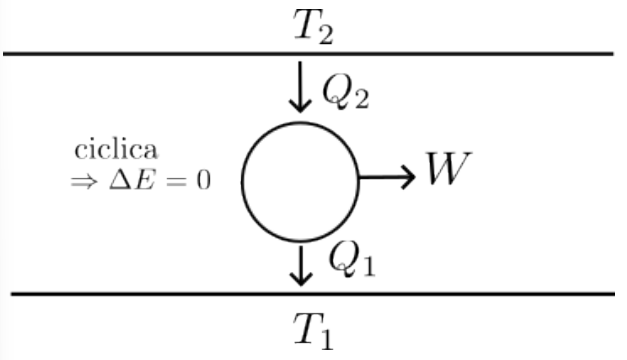
\includegraphics[width=0.4\linewidth]{Immagini/macchina di Carnot 1.png}
    \caption{macchina ciclica reversibile con $T_2 > T_1$.}
    \label{fig: macchina di Carnot 1}
\end{figure}

Per il secondo principio della Termodinamica (\ref{axiom: I principio della TD}), dato che la variazione di energia di una macchina ciclica è $\Delta E = 0$, il lavoro $W$ coincide con $W = Q_2 - Q_1$, per cui il rendimento $\eta$ della macchina in questione è
\begin{equation}
\label{eq: rendimento macchina ciclica reversibile}
    \eta = \frac{W}{Q_2} = \frac{Q_2 - Q_1}{Q_2} = 1 - \frac{Q_1}{Q_2} < 1,
\end{equation}
dove $Q_1 > 0$ per il primo principio della Termodinamica (\ref{axiom: II principio della TD, Clausius}). Un teorema fondamentale in Termodinamica, equivalente al secondo principio della Termodinamica, è il seguente.
\begin{teo}[di Carnot]
\label{teo: teorema di Carnot}
    Indicando con $R$ una generica macchina reversibile e con $I$ una generica macchina irreversibile, allora:
    \begin{enumerate}
        \item tutte le macchine termiche reversibili che utilizzano due sole sorgenti rispettivamente a temperatura $T_1$ e $T_2$ tali che $T_2 > T_1$, hanno lo stesso rendimento $\eta_R$ pari a quello di una macchina di Carnot che opera tra la medesima coppia di sorgenti, ovvero $\eta_R = \eta_C$;
        \item le macchine termiche irreversibili che utilizzano due sole sorgenti rispettivamente a temperatura $T_1$ e $T_2$ tali che $T_2 > T_1$, hanno un rendimento $\eta_I$ sempre minore di una macchina reversibile che opera tra la medesima coppia di sorgenti, ovvero $\eta_I < \eta_R$.
    \end{enumerate}
\end{teo}
La dimostrazione del teorema \ref{teo: teorema di Carnot} procede per assurdo ma si omette in questa sede. Dallo stesso segue che $\eta_R$ è lo stesso per tutte le macchine reversibili operanti tra $T_2$ e $T_1$, per cui
\begin{equation}
\label{eq: rapporto calori macchina reversibile}
    \frac{Q_{1R}}{Q_{2R}}=f(T_2,T_1),
\end{equation}
ossia il rapporto tra il calore assorbito e ceduto da una macchina reversibile deve essere esprimibile come una funzione dipendente solo dalla temperature delle sorgenti.

Fino ad ora si è dato per scontato che la scala della temperatura fosse quella assoluta $T$. Tuttavia, in linea di principio, si può utilizzare qualsiasi scala di temperatura $t$. A partire da questo, si può ottenere univocamente una temperatura termodinamica sfruttando le proprietà dei cicli di Carnot.
\begin{figure}[h]
    \centering
    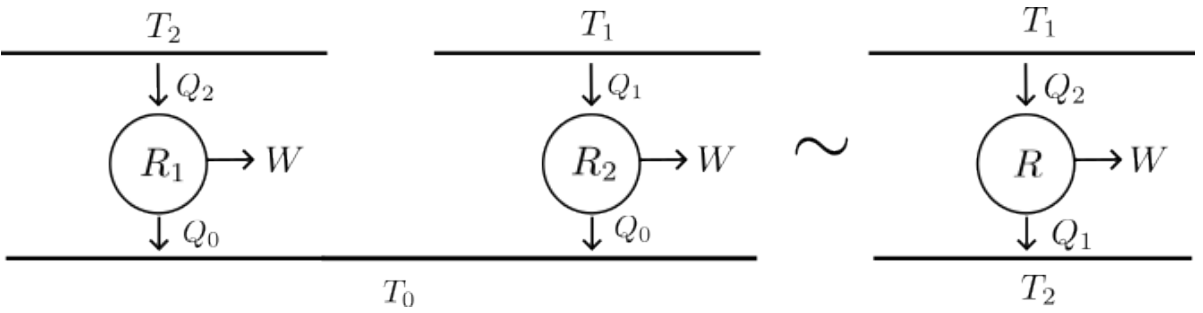
\includegraphics[width=0.8\linewidth]{Immagini/coppia macchine di Carnot.png}
    \caption{combinazione di due macchine cicliche reversibili.}
    \label{fig: coppia macchine di Carnot}
\end{figure}
Quindi, combinando due cicli di Carnot $R_1$ ed $R_2$, il primo operante tra $t_2$ e $t_0$, mentre il secondo tra $t_1$ e $t_0$, se ne può ottenere un  terzo operante tra $t_2$ e $t_1$, come mostrato in figura \ref{fig: coppia macchine di Carnot}. In base alla \eqref{eq: rapporto calori macchina reversibile}, si ha
\begin{equation}
\label{eq: rapporti calori macchine reversibili}
    \frac{Q_0}{Q_2}=f(t_2,t_0),\quad\frac{Q_0}{Q_1}=f(t_1,t_0),\quad\frac{Q_1}{Q_2}=f(t_2,t_1),
\end{equation}
ma allora scrivendo il rapporto tra calore assorbito e scambiato per il terzo ciclo come
\begin{equation}
    \frac{Q_1}{Q_2}=\frac{Q_1}{Q_0}\frac{Q_0}{Q_2},
\end{equation}
si trova la relazione
\begin{equation}
\label{eq: equazione funzionale per f}
    f(t_2,t_1)=\frac{f(t_2,t_0)}{f(t_1,t_0)},
\end{equation}
la cui soluzione generale è
\begin{equation}
\label{eq: soluzione generale per f}
    f(t_2,t_1)=\frac{\theta(t_2)}{\theta(t_1)},
\end{equation}
dove $\theta(t)$ è in generale una funzione della temperatura $t$ utilizzata, deducibile dal rendimento dei cicli di Carnot. Si può allora definire una temperatura termodinamica $T$ proporzionale a $\theta(t)$, cioè tale che 
\begin{equation}
\label{eq: definizione temperatura assoluta}
    f(t_2,t_1)=\frac{T_2}{T_1}.
\end{equation}
In questo modo si definisce $T$ a meno di una costante moltiplicativa che può essere fissata convenzionalmente imponendo $\Delta T = 100$ tra i due punti di fusione ed ebollizione dell'acqua a pressione standard. Si può mostrare che questa definizione coincide con la temperatura assoluta definita tramite il termometro a gas perfetto. Tramite le equazioni \eqref{eq: rendimento macchina ciclica reversibile}, \eqref{eq: rapporto calori macchina reversibile} e \eqref{eq: rapporti calori macchine reversibili} si può scrivere il rendimento di una macchina reversibile come 
\begin{equation}
\label{eq: rendimento macchina ciclica reversibile in funzione di T}
    \eta_R=1-\frac{\theta(t_1)}{\theta(t_2)}=1-\frac{T_1}{T_2}.
\end{equation}
Usando da qui in avanti la convezione che il calore assorbito dal sistema ha segno negativo, si considera una macchina operante tra due sorgenti di temperatura $T_2$ e $T_1$ rispettivamente, tali che ora $T_2 < T_1$, come mostrato in figura \ref{fig: macchina di Carnot 2}.
\begin{figure}[h]
    \centering
    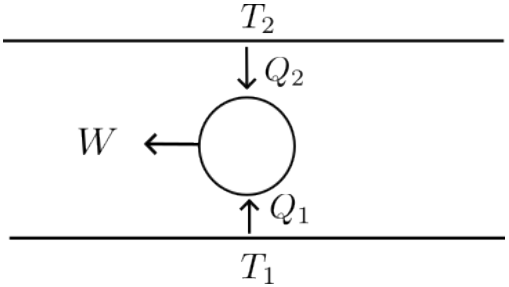
\includegraphics[width=0.4\linewidth]{Immagini/macchina di Carnot 2.png}
    \caption{macchina ciclica reversibile con $T_2 < T_1$.}
    \label{fig: macchina di Carnot 2}
\end{figure}

Combinando le equazioni \eqref{eq: rendimento macchina ciclica reversibile} e \eqref{eq: rendimento macchina ciclica reversibile in funzione di T} si ottiene la disuguaglianza
\begin{equation}
    1 + \frac{Q_1}{Q_2} \le 1 - \frac{T_1}{T_2},
\end{equation}
da cui, se arrangiata opportunamente, si ricava la disuguaglianza di Clausius
\begin{equation}
\label{eq: disuguaglianza di Clausius}
    \frac{Q_1}{T_1} + \frac{Q_2}{T_2} \le 0,
\end{equation}
dove $Q_1 < 0$ per il secondo principio della Termodinamica. La disuguaglianza \eqref{eq: disuguaglianza di Clausius} si può generalizzare ad un numero $n$ di sorgenti con
\begin{equation}
\label{eq: disuguaglianza di Clausius n sorgenti}
    \sum_{i=1}^n\frac{Q_i}{T_i} \le 0,
\end{equation}
e, analogamente, ad un ciclo termodinamico generico, approssimandolo ad una serie di trasformazioni adiabatiche isoterme, con
\begin{equation}
\label{eq: disuguaglianza di Clausius ciclo termodinamico}
    \oint_C\frac{\delta Q}{T} \le 0.
\end{equation}
In particolare, se il ciclo è reversibile, allora
\begin{equation}
\label{eq: disuguaglianza di Clausius ciclo reversibile}
    \oint_C\frac{\delta Q}{T}=0\quad\Rightarrow\quad\frac{\delta Q}{T} = dS,
\end{equation}
dove $dS$ è un differenziale esatto. La funzione di $S$ prende il nome di entropia ed è una funzione di stato, per cui dati due stati diversi $A$ e $B$, la variazione di entropia necessaria per passare da $A$ a $B$ non dipende dal percorso scelto, ossia
\begin{equation}
\label{eq: proprietà funzione di stato entropia}
    \Delta S_{AB} = S_B - S_A.
\end{equation}
Facendo riferimento al ciclo mostrato in figura \ref{fig: ciclo termodinamico generico}, è possibile applicare l'equazione \eqref{eq: disuguaglianza di Clausius ciclo termodinamico} ottenendo
\begin{equation}
    \begin{split}
        \int_A^B\frac{\delta Q_I}{T} + \int_B^A\frac{\delta Q_R}{T} &< 0 \\
        \int_A^B\frac{\delta Q_I}{T} + \int_B^AdS &<0 \\
        \int_A^B\frac{\delta Q_I}{T} + \Delta S_{BA} &< 0 \\
        \int_A^B\frac{\delta Q_I}{T} &< \Delta S_{AB}.
    \end{split}
\end{equation}
Quindi, per un tratto infinitesimo la variazione di entropia è
\begin{equation}
\label{eq: variazione di entropia infinitesima}
    dS = \frac{\delta Q_I}{T} + \delta S_I,\quad \delta S_I > 0,
\end{equation}
dove $\delta S_I$ è la parte di variazione entropica non spiegata dal flusso di calore, legata invece all'aumento del disordine microscopico.
\begin{figure}[h]
    \centering
    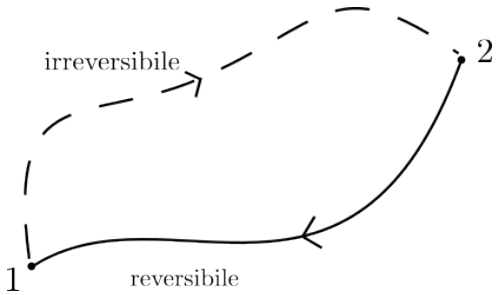
\includegraphics[width=0.4\linewidth]{Immagini/ciclo termodinamico generico.png}
    \caption{ciclo termodinamico generico.}
    \label{fig: ciclo termodinamico generico}
\end{figure}

In particolare, per processi spontanei, ovvero adiabatici (con $\delta Q = 0$) e irreversibili, la variazione di entropia è
\begin{equation}
    dS = \delta S_I > 0,
\end{equation}
una relazione equivalente al secondo principio della Termodinamica. Inoltre, dire che uno stato di equilibrio è stabile rispetto a fluttuazioni spontanee equivale a dire che coincide con un massimo dell'entropia. Una proprietà importante dell'entropia è l'essere estensiva, essendo una funzione dipendente dal calore $Q$, estensivo, e dalla temperatura $T$, intensiva. Combinando le equazioni \eqref{eq: combinazione espressione lavoro e I PDT} e \eqref{eq: disuguaglianza di Clausius} si ottiene
\begin{equation}
\label{eq: disuguaglianza tra TdS e dE}
    TdS \ge dE + pdV -\mu dN - ydx,
\end{equation}
dove il caso di uguaglianza si presenta se il ciclo è reversibile e vale \eqref{eq: disuguaglianza di Clausius ciclo reversibile}. 

Ad ogni modo, l'entropia si dice essere una funzione estensiva di variabili estensive\footnote{Per semplicità si evita spesso di evidenziare la dipendenza dagli spostamenti generalizzati $X$.}, effettivamente $S \equiv S(E,V,N,X)$. Quindi, conoscere $S$ equivale a conoscere le equazioni di stato, infatti
\begin{align}
\label{eq: equazioni di stato da S}
    \frac{\p S}{\p E}\bigg|_{V,N,X}&=\frac{1}{T},\quad\mathrm{(equazione\,di\,stato\,termica)}, \\
    \frac{\p S}{\p N}\bigg|_{E,V,X}&=-\frac{\mu}{T},\quad\mathrm{(equazione\,di\,stato\,chimica)}, \\
    \frac{\p S}{\p V}\bigg|_{E,N,X}&=\frac{p}{T},\quad\mathrm{(equazione\,di\,stato\,meccanica)}, \\
    \frac{\p S}{\p X}\bigg|_{E,V,N}&=-\frac{y}{T},\quad\mathrm{(equazione\,di\,stato\,generalizzata)}.
\end{align}
\begin{obs}
    In Termodinamica, le espressioni delle equazioni di stato sono ricavate ``sperimentalmente'' e da esse si ricava l'espressione di $S(E,V,N,X)$. Invece, in Meccanica statistica si deriva prima $S(E,V,N,X)$ per poi derivare le equazioni \eqref{eq: equazioni di stato da S}. 
\end{obs}
La caratteristica dell'entropia di funzione estensiva di variabili estensive implica che se si scalano le grandezze da cui $S$ dipende di un fattore reale $\lambda$ si ha
\begin{equation}
\label{eq: S funzione omogenea di I grado}
    S(\lambda E,\lambda V,\lambda N,\lambda X) = \lambda S(E,V,N,X),\quad \lambda\in\R^+.
\end{equation}
L'equazione \eqref{eq: S funzione omogenea di I grado} implica che $S$ è una funzione omogenea di primo grado\footnote{In generale, una funzione $f(x_i)$ si dice omogenea di grado $d$ se soddisfa la relazione $f(\lambda x_i) = \lambda^d f(x_i)$ e se è autofunzione dell'operatore di Eulero $D=\nsum_ix^i\p_{x_i}$, ossia se $Df(x_i)=df(x_i)$.} nelle sue variabili. Dunque, nel caso dell'entropia si ha
\begin{multline}
    S = E\bigg(\frac{\p S}{\p E}\bigg|_{V,N,X}\bigg) + V\bigg(\frac{\p S}{\p V}\bigg|_{E,N,X}\bigg) + \\
    + N\bigg(\frac{\p S}{\p N}\bigg|_{E,V,X}\bigg) + X\bigg(\frac{\p S}{\p X}\bigg|_{E,V,N}\bigg),
\end{multline}
che, se si sostituiscono le equazioni \eqref{eq: equazioni di stato da S} e si moltiplica per $T$, si ricava l'equazione fondamentale della Termodinamica
\begin{equation}
\label{eq: equazioni fondamentale della TD}
    TS = E + pV - \mu N - yX.
\end{equation}
\begin{obs}
    L'equazione \eqref{eq: equazioni fondamentale della TD} potrebbe sembrare l'integrale ``sbagliato'' dell'equazione \eqref{eq: disuguaglianza tra TdS e dE}, ma in realtà è corretto dato che $S$ è una funzione omogenea di primo grado.    
\end{obs}
Differenziando l'equazione \eqref{eq: equazioni fondamentale della TD} e sostituendo la \eqref{eq: disuguaglianza tra TdS e dE} nel caso reversibile si ottiene l'equazione di Gibbs-Duhem
\begin{equation}
\label{eq: equazione di Gibbs-Duhem}
    SdT = Vdp - Nd\mu - Xdy.
\end{equation}
Invertendo $S(E,V,N,X)$ si può vedere l'energia $E$ come funzione di variabili estensive $E\equiv E(S,V,N,X)$, dall'equazione di stato termica in \eqref{eq: equazioni di stato da S} segue che
\begin{equation}
    \frac{\p E}{\p S}\bigg|_{V,N,X}=T.
\end{equation}
Ricordando la relazione \eqref{eq: disuguaglianza tra TdS e dE} si deduce che per sistemi chiusi, ovvero tali che $dN = 0$, a cui non viene fornito calore in modo reversibile, ovvero $dS = 0$, isocoro, ovvero con $dV = 0$, e con tutte le altri variabili estensive fisse, ovvero $dX = 0$, per ogni trasformazione si ha 
\begin{equation}
    dE \le 0,
\end{equation}
per cui il sistema evolve verso uno stato di equilibrio coincidente con un minimo di energia. L'energia interna $E$ gioca dunque un ruolo analogo all'energia potenziale in Meccanica quando le variabili di controllo del sistema sono $\{S,V,N,X\}$. In tal caso, le funzioni estensive come l'energia $E$ sono funzioni omogenee di primo grado e quindi
\begin{equation}
\label{eq: equazioni di stato da E}
    \begin{split}
         T=\frac{\p E}{\p S}\bigg|_{V,N,X}&,\quad p=-\frac{\p E}{\p V}\bigg|_{S,N,X}, \\
         \mu=\frac{\p E}{\p N}\bigg|_{S,V,X}&,\quad y=\frac{\p E}{\p X}\bigg|_{S,V,N},
    \end{split}
\end{equation}
che sono funzioni omogenee di grado zero come è evidente da queste relazioni, ad esempio
\begin{equation}
    p(\lambda S,\lambda V,\lambda N,\lambda X) = p(S,V,N,X),\quad\lambda\in\R^+.
\end{equation}
In particolare, scegliendo $\lambda = 1/N$ si ha 
\begin{equation}
    p(\lambda S,\lambda V,\lambda N,\lambda X) = p(s,v,n,x) \equiv p(s,v,x),
\end{equation}
dove $s = S/N$, $v = V/N$ e $x = X/N$ sono l'entropia, il volume e lo spostamento generalizzato della singola componente. Se quindi si hanno $3 + r$ variabili estensive indipendenti quali $S$, $V$, $N$ e gli $r$ spostamenti $X$, le grandezze intensive a loro coniugate sono solo $2 + r$ rapporti indipendenti di tali variabili.

Potrebbe essere conveniente usare un insieme di variabili di controllo che contengono alcune delle variabili intensive $T$, $p$, $\mu$ e $y$, che in termini di $E$ sono espresse dalle equazioni \eqref{eq: equazioni di stato da E}. La tecnica matematica necessaria per passare dalle variabili estensive alle loro coniugate intensive è la trasformata di Legendre\footnote{\'E la stessa trasformata che viene applicata per passare dalla descrizione lagrangiana a quella hamiltoniana.}. In questo modo si definiscono altri potenziali termodinamici adatti a diversi insiemi di variabili di controllo. 

\paragraph{Energia libera di Helmoltz.} Applicando la trasformata di Legendre rispetto alla coppia di variabili $(T=\p_S E,S)$ si ottiene
\begin{equation}
\label{eq: TdL rispetto a (T,S)}
    F(T,V,N,X) = E(S,V,N,X) - TS,
\end{equation}
dove nel secondo membro $S$ è pensata come dipendente ed ottenuta invertendo la relazione $T=\p_S E$. Usando l'equazione fondamentale \eqref{eq: equazioni fondamentale della TD} si può scrivere
\begin{equation}
\label{eq: espressione di F}
    F = -pV + \mu N + yX.
\end{equation}
Ora differenziando l'equazione \eqref{eq: TdL rispetto a (T,S)} e tenendo conto della \eqref{eq: disuguaglianza tra TdS e dE} si ottiene
\begin{equation}
    dF \le -SdT -pdV + \mu dN + ydX.
\end{equation}
Per un sistema chiuso ($dN = 0$), a temperatura costante ($dT = 0$), a volume costante ($dV = 0$) e con tutte le altre variabili estensive fisse ($dX = 0$), per ogni trasformazione si ha
\begin{equation}
    dF \le 0,
\end{equation}
per cui il sistema evolve verso uno stato di equilibrio coincidente con un minimo di $F$ che prende il nome di energia libera di Helmoltz. Le variabili dipendenti in questo caso sono 
\begin{equation}
\label{eq: equazioni di stato da F}
    \begin{split}
        S = -\frac{\p F}{\p T}\bigg|_{V,N,X}&,\quad p = -\frac{\p F}{\p V}\bigg|_{T,N,X}, \\
        \mu = \frac{\p F}{\p N}\bigg|_{T,V,X}&,\quad y = \frac{\p F}{\p X}\bigg|_{T,V,N}.
    \end{split}
\end{equation}
\paragraph{Entalpia.} Applicando la trasformata di Legendre alla coppia di variabili $(p = -\p_V E,V)$ si ottiene
\begin{equation}
\label{eq: TdL rispetto a (p,V)}
    H(S,p,N,X) = E(S,V,N,X) + pV,
\end{equation}
dove nel secondo membro $V$ è pensato come dipendente ed ottenuto invertendo l'equazione di stato meccanica $p = -\p_V E$. Usando l'equazione fondamentale \eqref{eq: equazioni fondamentale della TD} si può scrivere 
\begin{equation}
\label{eq: espressione di H}
    H = TS + \mu N + yX.
\end{equation}
Ora differenziando l'equazione \eqref{eq: TdL rispetto a (p,V)} e tenendo conto della \eqref{eq: disuguaglianza tra TdS e dE} si ottiene
\begin{equation}
    dH \le TdS + Vdp +\mu dN +ydX.
\end{equation}
Per un sistema chiuso ($dN = 0$), in condizioni isoentorpiche ($dS = 0$), ossia senza trasferimento reversibile di calore, a pressione costante ($dp = 0$) e con tutte le altre variabili estensive fisse ($dX = 0$), per ogni trasformazione si ha
\begin{equation}
    dH \le 0,
\end{equation}
per cui il sistema evolve verso uno stato di equilibrio coincidente con un minimo di $H$ che prende il nome di entalpia. Le variabili dipendenti in questo caso sono 
\begin{equation}
\label{eq: equazioni di stato da H}
    \begin{split}
        T = \frac{\p H}{\p S}\bigg|_{p,N,X}&,\quad V = \frac{\p H}{\p p}\bigg|_{S,N,X}, \\
        \mu = \frac{\p H}{\p N}\bigg|_{S,p,X}&,\quad y = \frac{\p H}{\p X}\bigg|_{S,p,N}.
    \end{split}
\end{equation}

\paragraph{Energia libera di Gibbs.} Applicando la trasformata di Legendre sia alla coppia di variabili $(-p,V)$ che alla coppia $(T,S)$ si ottiene
\begin{equation}
\label{eq: TdL rispetto a (-p,V) e a (T,S)}
    G(T,p,N,X) = E(S,V,N,X) - TS +pV,
\end{equation}
dove $S$ e $V$ sono pensate come dipendenti ed ottenute invertendo le equazioni di stato rispettive tra le \eqref{eq: equazioni di stato da E}. Usando l'equazione fondamentale \eqref{eq: equazioni fondamentale della TD} si può riscrivere
\begin{equation}
\label{eq: espressione di G}
    G = \mu N + yX,
\end{equation}
che si riduce a $G = \mu N$ se nel sistema non compaiono variabili $(y,X)$. Differenziando la \eqref{eq: TdL rispetto a (-p,V) e a (T,S)} e tenendo conto della \eqref{eq: disuguaglianza tra TdS e dE} si ottiene
\begin{equation}
    dG \le -SdT + Vdp +\mu dN +ydX.
\end{equation}
Per un sistema chiuso ($dN = 0$), a pressione costante ($dp = 0$), a temperatura costante ($dT = 0$) e con tutte le altre variabili estensive fisse ($dX = 0$), per ogni trasformazione si ha
\begin{equation}
    dG \le 0,
\end{equation}
per cui ogni sistema evolve verso uno stato di equilibrio coincidente con un minimo di $G$ che prende il nome di energia libera di Gibbs. Le variabili dipendenti in questo caso sono
\begin{equation}
\label{eq: equazioni di stato da G}
    \begin{split}
        S = -\frac{\p G}{\p T}\bigg|_{p,N,X}&,\quad V = \frac{\p G}{\p p}\bigg|_{T,N,X}, \\
        \mu = \frac{\p G}{\p N}\bigg|_{T,p,X}&,\quad y = \frac{\p G}{\p X}\bigg|_{T,p,N}.
    \end{split}
\end{equation}

\paragraph{Potenziale grancanonico.} Applicando la trasformata di Legendre sia alla coppia di variabili $(T,S)$ che alla coppia $(\mu,N)$ si ottiene
\begin{equation}
\label{eq: TdL rispetto a (T,S) e (mu,N)}
    \varpi(T,V,\mu,X) = E(S,V,N,X) - TS - \mu N,
\end{equation}
dove $S$ ed $N$ sono pensate come indipendenti ed ottenute invertendo le equazioni di stato rispettive tra le \eqref{eq: equazioni di stato da E}. Usando l'equazione fondamentale \eqref{eq: equazioni fondamentale della TD} si può riscrivere 
\begin{equation}
\label{eq: espressione del pot. grancanonico}
    \varpi = -pV + yX,
\end{equation}
che si riduce a $\varpi =  -pV$ se nel sistema non compaiono variabili $(y,X)$. Differenziando la \eqref{eq: TdL rispetto a (T,S) e (mu,N)} e tenendo conto della \eqref{eq: disuguaglianza tra TdS e dE} si ottiene
\begin{equation}
    d\varpi \le -SdT -pdV - N\mu +ydX.
\end{equation}
Per un sistema aperto, ma a potenziale chimico costante ($d\mu = 0$), a temperatura costante ($dT = 0$), in condizioni isobariche ($dV = 0$) e con tutte le altr variabili estensive fisse ($dX = 0$), per ogni trasformazioni si ha
\begin{equation}
    d\varpi \le 0,
\end{equation}
per cui ogni sistema evolve verso uno stato di equilibrio coincidente con un minimo di $\varpi$ che prende il nome di potenziale grancanonico. Le variabili indipendenti in questo caso sono
\begin{equation}
\label{eq: equazioni di stato dapot. grancanonico}
    \begin{split}
        S = -\frac{\p \varpi}{\p T}\bigg|_{V,\mu,X}&,\quad p = -\frac{\p \varpi}{\p V}\bigg|_{T,\mu,X}, \\
        N = \frac{\p \varpi}{\p \mu}\bigg|_{T,V,X}&,\quad y = \frac{\p \varpi}{\p X}\bigg|_{T,V,\mu}.
    \end{split}
\end{equation}

\paragraph{Potenziali generali.} In linea di principio è possibile ottenere, a partire dai precedenti, ulteriori potenziali applicando la trasformata di Legendre rispetto alle coppie, alcune o tutte, di variabili $(y,X)$. Per tali potenziali non esistono nomi specifici; tuttavia, possono essere quelli convenienti in date situazioni in cui le variabili tra le di controllo compaiono alcune delle $y$. In particolare, se a partire da $G$ si applica la trasformata di Legendre rispetto a tutte le coppie $(y,X)$ si ottiene
\begin{equation}
    \tilde{G}(T,p,N,y) = G(T,p,N,X) -yX,
\end{equation}
dove $X$ è vista come indipendente ottenuta invertendo la relazione rispettiva tra le \eqref{eq: equazioni di stato da G}. Dalla \eqref{eq: espressione di G} segue che 
\begin{equation}
    \tilde{G} = \mu N,
\end{equation}
e quindi il potenziale specifico $\tilde{g} = \tilde{G}/N$ coincide proprio con il potenziale chimico $\mu$. Allo stesso modo si può ragionare per $\varpi$ ottenendo 
\begin{equation}
    \tilde{\varpi}(T,V,\mu,y) = \varpi(T,V,\mu,X) - yX
\end{equation}
e dalla \eqref{eq: espressione del pot. grancanonico} segue che
\begin{equation}
    \tilde{\varpi} = -pV
\end{equation}
e quindi la densità di potenziale $\tilde{\varpi}/V$ coincide con $-p$.

\section{Funzioni di risposta} 
Le funzioni di risposta sono quantità che descrivono come una data funzione di stato cambi al variare di un'altra variabili indipendente in condizioni controllate; in particolare, è interessante il caso in cui le due variabili sono coniugate. Inoltre, sono le quantità più direttamente misurabili sperimentalmente. Sono legate poi, dal punto di vista macroscopico, alla grandezza delle fluttuazioni del sistema. Le funzioni di risposta si dividono in due grandi categorie: termiche e meccaniche. Si considerano nel seguito alcune delle più importanti.

\subsubsection{Capacità termica}
La capacità termica misura la quantità di calore che è necessario fornire ad un sistema per variarne la temperatura di una quantità fissata, per cui la definizione generale è
\begin{equation}
    c = \frac{\delta Q}{dT}.
\end{equation}
Dato che $\delta Q$ non è un differenziale è necessario specificare il tipo di trasformazione con cui il calore viene fornito.

Se $\delta W = pdV - \mu dN - ydX  = 0$, allora dal primo principio della Termodinamica si ha $\delta Q = dE$, per cui si definisce la capacità termica a volume costante $c_V$ come
\begin{equation}
\label{eq: capacità termica V costante}
    c_{V,N,X} \equiv c_V = \frac{\p E}{\p T}\bigg|_{V,N,X}.
\end{equation}
Si può esprimere \eqref{eq: capacità termica V costante} anche in funzione dell'entropia usando $\delta Q = TdS$; se questo è il caso, allora si stanno usando come variabili indipendenti $\{T,V,N.X\}$ le cui ultime tre sono fisse, per cui 
\begin{equation}
    dS = \frac{\p S}{\p T}\bigg|_{V,N,X}dT
\end{equation}
e quindi
\begin{equation}
    c_V = T\frac{dS}{dT} = T\frac{\p S}{\p T}\bigg|_{V,N,X}.
\end{equation}
Avendo come variabili indipendenti $\{T,V,N,X\}$ il potenziale rilevante è l'energia libera di Helmoltz $F(T,V,N,X)$ e l'entropia è vista come
\begin{equation}
    S = -\frac{\p F}{\p T}\bigg|_{V,N,X},
\end{equation}
quindi si può scrivere
\begin{equation}
    c_V = -T\frac{\p^2F}{\p T^2}\bigg|_{V,N,X}
\end{equation}

Se invece $\delta W = pdV$, allora sempre dal primo principio della Termodinamica si ha $\delta Q = dE + pdV$, per cui si definisce al capacità termica a pressione costante $c_p$ come 
\begin{equation}
\label{eq: capacità termica p costante}
    c_{p,V,X} \equiv c_p = \frac{\p E}{\p T}\bigg|_{p,N,X} + p\frac{\p V}{\p T}\bigg|_{p,N,X}.
\end{equation}
Avendo come variabili di indipendenti $\{T,p,N,X\}$ il potenziale rilevante è l'energia libera di Gibbs $G(T,p,N,X)$ e l'energia è vista come
\begin{equation}
    E = G + TS -pV = G - T\frac{\p G}{\p T} - pV,
\end{equation}
dove si sono usate le relazioni \eqref{eq: equazioni di stato da G}, che sostituita nella \eqref{eq: capacità termica p costante} restituisce
\begin{equation}
    \begin{split}
        c_p &= \frac{\p}{\p T}\bigg(G - T\frac{\p G}{\p T} - pV\bigg)\bigg|_{p,N,X} + p\frac{\p V}{\p T}\bigg|_{p,N,X} \\
        &=\bigg(\frac{\p G}{\p T} - \frac{\p G}{\p T} -T\frac{\p^2G}{\p T^2}\bigg)\bigg|_{p,N,X} \\
        &=-T\frac{\p^2 G}{\p T^2}\bigg|_{p,N,X}.
    \end{split}
\end{equation}
Il medesimo risultato si può ottenere a partire da $\delta Q = TdS$.

\subsubsection{Suscettività termica}
La suscettività di un sistema indica di quanto il volume aumenta al crescere delle pressione. Dato che ciò può essere effettuato in modi diversi è necessario specificare il tipo di trasformazione, in particolare indicando quali variabili vengono mantenute costanti.

Se si mantengono costanti le variabili $\{T,N,X\}$, allora si definisce la suscettività isoterma $\chi_T$ come
\begin{equation}
    \chi_T = -\frac{\p V}{\p p}\bigg|_{T,N,X}.
\end{equation}
Se le variabili indipendenti sono $\{T,p,N,X\}$, allora il potenziale rilevante è l'energia libera di Gibbs $G$, per cui esprimendo $V$ tramite l'equazione rispettiva tra le \eqref{eq: equazioni di stato da G} si ha
\begin{equation}
    \chi_T = -\frac{\p^2 G}{\p p^2}\bigg|_{T,N,X}. 
\end{equation}

Se invece si mantengono costanti le variabili $\{S,N,X\}$, allora si definisce la suscettività adiabatica come
\begin{equation}
    \chi_S = -\frac{\p V}{\p p}\bigg|_{S,N,X}.
\end{equation}
Se le variabili indipendenti sono $\{S,p,N,X\}$, allora il potenziale rilevante è l'entalpia $H$, per cui esprimendo $V$ tramite l'equazione rispettiva tra le \eqref{eq: equazioni di stato da H} si ha
\begin{equation}
    \chi_S = -\frac{\p^2 H}{\p p^2}\bigg|_{S,N,X}.
\end{equation}

\subsubsection{Compressibilità termica}
La compressibilità di un sistema esprime la variazione percentuale di volume in seguito ad un cambiamento di pressione.

Se la variazione di pressione avviene mantenendo la temperatura $T$ costante, allora si definisce la compressibilità isoterma $\kappa_T$ come
\begin{equation}
    \kappa_T = \frac{\chi_T}{V} = -\frac{1}{V}\frac{\p^2 G}{\p p^2}\bigg|_{T,N,X}.
\end{equation}

Se invece la variazione di pressione avviene mantenendo l'entropia $S$ costante, allora si definisce la compressibilità adiabatica come 
\begin{equation}
    \kappa_S = \frac{\chi_S}{V} = -\frac{1}{V}\frac{\p^2 H}{\p p^2}\bigg|_{S,N,X}
\end{equation}

\subsubsection{Espansibilità termica}
L'espansibilità termica descrive il cambiamento di volume in funzione della temperatura mantenendo costanti le variabili $\{p,N,X\}$, definita da
\begin{equation}
    \alpha_{p,N,X} \equiv \alpha_p = \frac{\p V}{\p T}\bigg|_{p,N,X}.
\end{equation}
In questo caso $V$ e $T$ non sono variabili coniugate, quindi $\alpha_p$ è collegata ad una derivata seconda mista del potenziale $G(T,p,N,X)$, infatti esprimendo $V$ con l'equazione rispettiva tra le \eqref{eq: equazioni di stato da G} si ha
\begin{equation}
    \alpha_p = \frac{\p^2 G}{\p p\p T}\bigg|_{N,X}.
\end{equation}

\section{Relazioni tra variabili}
In Termodinamica si ha continuamente a che fare con funzioni di molteplici variabili e con differenti scelte di set di variabili. Alcune identità matematiche forniscono delle relazioni utili per svariate grandezze termodinamiche.

Innanzitutto, l'ordine della derivazione parziale di una funzione non conta, ossia
\begin{equation}
\label{eq: ordine derivate parziali irrilevante}
    \frac{\p^2 f}{\p x^i\p x^j} = \frac{\p^2 f}{\p x^j \p x^i},
\end{equation}
e questo si estende a derivate parziali di ordine superiore. Si considerino ora tre variabili $x$, $y$ e $z$ legate da una relazione del tipo $f(x,y,z) = 0$, per cui si può scegliere arbitrariamente due di esse come indipendenti. In questo modo, si hanno
\begin{equation}
    \frac{\p x}{\p y}\bigg|_z = \bigg(\frac{\p y}{\p x}\bigg|_z\bigg)^{-1},\quad\frac{\p x}{\p y}\bigg|_z\frac{\p y}{\p z}\bigg|_x\frac{\p z}{\p x}\bigg|_y = -1.
\end{equation}
Si consideri un'ulteriore funzione $w\equiv w(x,y,z)$ con due delle variabili da cui dipende sempre scelte arbitrariamente indipendenti, così si hanno
\begin{equation}
    \frac{\p x}{\p w}\bigg|_z = \frac{\p x}{\p y}\bigg|_z\frac{\p y}{\p w}\bigg|_z,\quad\frac{\p x}{\p y}\bigg|_z = \frac{\p x}{\p y}\bigg|_w + \frac{\p x}{\p w}\bigg|_y\frac{\p w}{\p y}\bigg|_z.
\end{equation}

A partire dalle equazioni di stato \eqref{eq: equazioni di stato da E} che definiscono le variabili intensive in termini di $E$, usando la \eqref{eq: ordine derivate parziali irrilevante}, si ha
\begin{equation}
    \frac{\p T}{\p V}\bigg|_{S,N,X} = \frac{\p^2 E}{\p V\p S}\bigg|_{N,X} = \frac{\p}{\p S}\bigg(\frac{\p E}{\p V}\bigg|_{N,X}\bigg) = -\frac{\p p}{\p S}\bigg|_{V,N,X}.
\end{equation}
In modo analogo, si hanno
\begin{align}
    \frac{\p T}{\p N}\bigg|_{S,V,X} &= \frac{\p^2 E}{\p N\p S}\bigg|_{N,X} = \frac{\p\mu}{\p S}\bigg|_{N,X}, \\
    \frac{\p T}{\p X}\bigg|_{S,V,N} &= \frac{\p^2 E}{\p X\p S}\bigg|_{V,N} = \frac{\p y}{\p S}\bigg|_{V,N,X}, \\
    \frac{\p p}{\p N}\bigg|_{S,V,X} &= -\frac{\p^2 E}{\p N\p V}\bigg|_{S,X} = -\frac{\p \mu}{\p V}\bigg|_{S,V,X}, \\
    \frac{\p p}{\p X}\bigg|_{S,V,N} &= -\frac{\p^2 E}{\p X\p V}\bigg|_{S,X} = -\frac{\p y}{\p V}\bigg|_{S,N,X}, \\
    \frac{\p \mu}{\p X}\bigg|_{S,N,V} &= \frac{\p^2 E}{\p X\p N}\bigg|_{S,V} = \frac{\p y}{\p N}\bigg|_{S,V,X}.
\end{align}
Analoghe relazioni si possono trovare a partire dagli altri potenziali termodinamici, cioè da altri set di  variabili indipendenti. La regola generale è la seguente. Se $\{z_i\}$ è l'insieme di variabili indipendenti scelto e $\{\zeta_i\}$ sono le variabili coniugate, in modo che il potenziale appropriato sia
\begin{equation}
    d\Phi = \nsum_i\zeta_idz_i,
\end{equation}
allora
\begin{equation}
    \frac{\p\zeta_A}{\p z_B}\bigg|_{\{z_i\}\setminus z_B} = \frac{\p^2\Phi}{\p z_B \p z_A}\bigg|_{\{z_i\}\setminus \{z_B,z_A\}} = \frac{\p \zeta_B}{\p z_A}\bigg|_{\{z_i\}\setminus z_B}.
\end{equation}

A partire dalle definizioni \eqref{eq: capacità termica V costante} e \eqref{eq: capacità termica p costante} si possono usare le identità matematiche elencate per ricavare una relazione tra $c_V$, $c_p$, $\chi_T$ e $\alpha_p$; questa è
\begin{equation}
    c_p = c_V + \frac{T}{\chi_T}\alpha_p^2.
\end{equation}




\chapter{Equilibrio termodinamico}
L'entropia di un sistema isolato è massima nel suo stato di equilibrio. Il sistema termodinamico è composto da un numero $N$ di componenti e le quantità termodinamiche rappresentano valori medi. Sono possibili quindi piccole fluttuazioni in tali valori. Da tali fluttuazioni l'entropia deve decrescere, altrimenti il sistema evolverebbe in un nuovo stato di equilibrio e quello precedente non sarebbe stabile. Da questo si possono dedurre importanti condizioni di equilibrio locale e di stabilità.
\begin{obs}
    Per semplicità, nel seguito ci si limita a considerare le coppie di variabili $(T,S)$, $(p,V)$ e $(\mu,N)$.
\end{obs}

\section{Equilibrio locale}
Si consideri un sistema isolato con $E$, $V$ ed $N$ fissati che si trovi in uno stato di equilibrio. Si supponga che in tale stato il sistema sia suddiviso in due parti $1$ e $2$ tali che 
\begin{equation}
    E = E_1 + E_2,\quad V = V_1 + V_2,\quad N = N_1 + N_2.
\end{equation}
Le due parti in cui è diviso il sistema possono essere ad esempio di un liquido oppure di una fase liquida in contatto con il suo vapore. La divisione in due parti può essere ideale o essere una parete mobile, induttiva e porosa. Si supponga ora che avvengano delle fluttuazioni spontanee $E_\alpha$, $V_\alpha$ ed $N_\alpha$ con i vincoli
\begin{equation}
\label{eq: vincoli variazioni sistema in due parti}
    \Delta E_2 = -\Delta E_1,\quad \Delta V_2 = -\Delta V_1,\quad \Delta N_2 = -\Delta N_1.
\end{equation}
Si assuma che le fluttuazioni siano piccole, in questo modo si può espandere al primo ordine il cambiamento di entropia dovuto a tali fluttuazioni
\begin{equation}
    \Delta S \simeq \sum_{\alpha = 1}^2\bigg[\frac{\p S}{\p E_\alpha}\bigg|_{V_\alpha,N_\alpha}^{eq}\Delta E_\alpha + \frac{\p S}{\p V_\alpha}\bigg|_{E_\alpha,N_\alpha}^{eq}\Delta V_\alpha + \frac{\p S}{\p N_\alpha}\bigg|_{E_\alpha,V_\alpha}^{eq}\Delta N_\alpha\bigg].
\end{equation}
Usando le equazioni di stato \eqref{eq: equazioni di stato da S} e le relazioni \eqref{eq: vincoli variazioni sistema in due parti} si ha
\begin{equation}
    \Delta S \simeq \bigg(\frac{1}{T_1^{eq}} - \frac{1}{T_2^{eq}}\bigg)\Delta E_1 + \bigg(\frac{p_1^{eq}}{T_1^{eq}} - \frac{p_2^{eq}}{T_2^{eq}}\bigg)\Delta V_1 - \bigg(\frac{\mu_1^{eq}}{T_1^{eq}} - \frac{\mu_2^{eq}}{T_2^{eq}}\bigg)\Delta N_1.
\end{equation}
Necessariamente, si deve avere $\Delta S \le 0$, ma $\Delta E_1$, $\Delta V_1$ e $\Delta N_1$ possono essere sia positivi che negativi, pertanto l'unico modo per non avere $\Delta S > 0$ è che siano vere
\begin{equation}
\label{eq: equilibrio termico sistema in due parti}
    T_1^{eq} = T_2^{{eq}},\quad p_1^{eq} = p_2^{eq},\quad \mu_1^{eq} = \mu_2^{eq},
\end{equation}
ovvero che il sistema sia in uno stato di equilibrio termico, meccanico e chimico tra le due parti. Inevitabilmente, si ha $\Delta S = 0$ al primo ordine nelle fluttuazioni. La discussione appena fatta per un sistema diviso in due parti può essere estesa ad un sistema diviso in $n$ parti richiedendo che le relazioni di equilibrio \eqref{eq: equilibrio termico sistema in due parti} siano valide per ognuna delle $n$ parti.

La condizione di equilibrio è sempre che $S$ sia massima, qualsiasi sia l'insieme di variabili di controllo scelte. A seconda di questo, la condizione di equilibrio può venire espressa come condizione di minimo per il potenziale di approccio. Ad esempio, per considerare le fluttuazioni di ripartizionamento di un sistema con $S$, $V$ e $N$ fissati, si può utilizzare l'energia interna $E(S, V, N)$ e richiedere che $\Delta E > 0$ per qualsiasi fluttuazione in queste condizioni. Con una trattazione del tutto analoga a quella fatta per $S(E, V, N)$ si trovano gli stessi risultati. All'equilibrio è necessario che siano verificate le equazioni \eqref{eq: equilibrio termico sistema in due parti} e che al primo ordine si abbia $\Delta E = 0$. Nell'analizzare i vincoli che emergono considerando il secondo ordine nelle piccoli fluttuazioni si è soliti sfruttare l'approccio in termini dei potenziali.

\subsection{Regola generale per i criteri di stabilità}
Si supponga che l'insieme delle variabili di controllo sia 
\begin{equation}
    \{X_1,\dots,X_{r},I_{r+1},\dots,I_n\},
\end{equation}
con le $X_i$ variabili estensive e le $I_j$ variabili intensive. Sia assuma inoltre che $\Phi(X_1,\dots,X_{r},I_{r+1},\dots,I_n)$ sia il potenziale appropriato, il cui differenziale è dato da
\begin{equation}
    d\Phi = \sum_{i = 1}^rI_idX_i - \sum_{j = r + 1}^nX_jdI_j.
\end{equation}
Lo stato di equilibrio è un minimo di $\Phi$, per cui per ogni fluttuazione si deve avere $\Delta\Phi \ge 0$. Si consideri quindi un partizionamento delle variabili estensive, ossia fluttuazioni tali che
\begin{equation}
    \delta X_i = \delta X_{i,1} + \delta X_{i,2} = 0.
\end{equation}
Al primo ordine nelle fluttuazioni si ha allora
\begin{equation}
    \Delta\Phi^{(1)} = \nsum_i\bigg[\frac{\p\Phi}{\p X_i}\bigg|_1 - \frac{\p\Phi}{\p X_i}\bigg|_2\bigg]\delta X_{i,1} \ge 0,
\end{equation}
con $\delta X_{i,1}$ senza vincoli, ossia che può essere sia positiva che negativa. Per assicurare la condizione di minimo $\Delta\Phi \ge 0$ si deve avere che
\begin{equation}
\label{eq: condizione equilibrio I ordine generale}
    \frac{\p\Phi}{\p X_i}\bigg|_1 = \frac{\p\Phi}{\p X_i}\bigg|_2\,\Longleftrightarrow\,I_{i,1} = I_{i,2},\quad\forall i.
\end{equation}
Questo si può generalizzare alla partizione in $n$ parti, giungendo alla conclusione che nello stato di equilibrio le variabili intensive dipendenti $I_i$ devono essere omogenee. Dalla condizione \eqref{eq: condizione equilibrio I ordine generale} necessariamente segue che al primo ordine nelle fluttuazioni si ha
\begin{equation}
    \Delta\Phi^{(1)} = 0,
\end{equation}
per cui al secondo ordine si deve avere $\Delta\Phi^{(2)} \ge 0$. Si considerino le fluttuazioni corrispondenti al ripartizionamento di una certa variabile estensiva $X_i$: essendo tutte indipendenti si possono considerare tali variazioni separatamente; quindi
\begin{equation}
\label{eq: condizioni equilibrio II ordine generale 0}
    \Delta\Phi^{(2)} = \frac{1}{2}\nsum_i\bigg[\frac{\p^2\Phi}{\p X_i^2}\bigg|_1 + \frac{\p^2\Phi}{\p X_i^2}\bigg|_2\bigg](\delta X_{i,1})^2 \ge 0.
\end{equation}
Essendo il partizionamento arbitrario, si deve avere in generale
\begin{equation}
\label{eq: condizione equilibrio II ordine generale 1}
    \frac{\p^2\Phi}{\p X_i^2}\bigg|_{1,2} = \frac{\p I_i}{\p X_i}\bigg|_{1,2} \ge 0.
\end{equation}
La stessa condizione si può interpretare il termini del potenziale $\tilde{\Phi}$, ottenuto da $\Phi$ applicando la trasformata di Legendre rispetto alla coppia di variabili $(I_i,X_i)$ data da $\tilde{\Phi}(\dots,I_i,\dots) = \Phi(\dots, X_i,\dots) - I_iX_i$, con
\begin{equation}
\label{eq: condizione equilibrio II ordine generale 2}
    \frac{\p X_i}{\p I_i} = -\frac{\p^2\tilde{\Phi}}{\p I_i^2}\quad\Rightarrow\quad\frac{\p^2\tilde{\Phi}}{\p I_i^2} \le 0.
\end{equation}
Scritte in questo modo, le condizioni di stabilità \eqref{eq: condizione equilibrio II ordine generale 1} e \eqref{eq: condizione equilibrio II ordine generale 2} corrispondono a richiedere che i potenziali rispettivi siano convessi o concavi.

\section{Sistemi multicomponenti}
Fino ad ora si sono considerati sistemi termodinamici composti da un unico tipo di costituenti elementari. Se invece si hanno $c$ tipi di costituenti diversi, distinti da un indice $a = 1,\dots,c$, ci sono allora $c$ coppie di variabili coniugate $(\mu_a,N_a)$, dove $N_a$ è il numero di componenti di tipo $a$ e $\mu_a$ il potenziale chimico per essi. I potenziali dipendono da $\mu_a$, o da $N_a$, per ogni $a$. Ad esempio, l'energia interna è $E(S,V,N_1,\dots,N_c,X)$ con 
\begin{equation}
    dE = TdS - pdV + \nsum_a\mu_adN_a + y dX.
\end{equation}
Il discorso è analogo per tutti gli potenziali. Le condizioni di equilibrio descritte da \eqref{eq: condizioni equilibrio II ordine generale 0}, per quanto riguarda i potenziali i potenziali chimici, diventano
\begin{equation}
    \mu_{a,1} = \mu_{a,2},\quad\forall a.
\end{equation}
Si noti anche che le grandezze intensive, che siano omogenee di grado zero, dipendono in realtà non da tutti gli $N_a$, ma dalle $c - 1$ frazioni indipendenti 
\begin{equation}
    \nu_a = \frac{N_a}{N},\quad N = \nsum_aN_a,
\end{equation}
con $N$ il numero totale di componenti, da cui segue che $\nsum_a\nu_a = 1$.

\subsection{Equilibrio delle fasi}
Lo stato di equilibrio di un sistema termodinamico è caratterizzato da poche grandezze indipendenti. Non è detto però che per qualsiasi insieme di valori $(E,V,\dots)$ lo stato di equilibrio debba essere omogeneo. Per certi intervalli può succedere che il sistema si separi in parti omogenee a contatto che si trovano in stati diversi, ossia con equazioni di stato diverse. Queste parti sono dette ``fasi''. Potrebbero esistere anche più di due fasi, ma anche considerandone solo due, non è detto che vi sia separazione in solo due regioni. In ogni caso, l'equilibrio termico fra le fasi richiede che $T_1 = \cdots = T_n$, ossia che $T$ sia omogenea in tutto il sistema. Analogamente, l'equilibrio meccanico fra le fasi richiede che $p_1 = \cdots = p_n$ e l'equilibrio chimico richiede che $\mu_1 = \cdots = \mu_n$. Limitandosi a sole due fasi, dato che $p$ e $T$ sono omogenee in tutto il sistema, si possono considerare come variabili di controllo. Le due fasi hanno proprietà diverse, quindi diverse equazioni di stato, cioè diverse  espressioni del potenziale di Gibbs: nella fase $\alpha$, con un numero di componenti $N_\alpha$, si ha un certo
\begin{equation}
    G_\alpha(T,p,N_\alpha) = \mu_\alpha N_\alpha.
\end{equation}

\subsubsection{Curve di coesistenza}
Per generici valori di $p$ e $T$ si ha $\mu_\alpha \neq \mu_\beta$ e lo stato di equilibrio è una o l'altra fase, per cui $N_\alpha = N$ oppure $N_\beta = N$, a seconda di quale corrisponde ad un minimo di $G$, ossia ad un minimo di $\mu = G/N$. La coesistenza richiede che 
\begin{equation}
\label{eq: condizione coesistenza}
    \mu_\alpha(p,T) = \mu_\beta(p,T).
\end{equation}
La separazione in fasi distinte in equilibrio fra di loro avviene dunque solo lungo una curva $p = p(T)$ detta ``curva di coesistenza''. Siccome $p$ e $T$ non sono variabili coniugate, la pendenza della curva di coesistenza non è fissata. Dunque, un tratto di tale curva può essere di due tipi:
\begin{enumerate}
    \item aumentando $p$ si passa dalla fase $\beta$ alla fase $\alpha$ e aumentando $T$ si passa dalla fase $\alpha$ alla fase $\beta$;
    \item aumentando $p$ si passa dalla fase $\alpha$ alla fase $\beta$ e aumentando $T$ si passa dalla fase $\alpha$ alla fase $\beta$.
\end{enumerate}

\subsection{Transizioni del primo ordine}
La curva di coesistenza tra due fasi $\alpha$ e $\beta$ è determinata dall'intersezione delle superfici
$\mu = \mu_\alpha(p,T)$ è $\mu = \mu_\beta(p,T)$. In generale, le derivate dei potenziali $\mu_\alpha$ e $\mu_\beta$ non coincidono all'intersezione, ad esempio tenendo costante la pressione $p$ si ha normalmente una situazione del tipo mostrata in figura \ref{fig: transizione I ordine p costante}. Dunque, in generale la derivata $\p_T\mu|_{p,N}$ è discontinua alla transizione. Siccome $\mu = G/N$ e $\p_TG|_{p,N} = -S$ si ha, in una fase $\alpha$, che
\begin{equation}
    \frac{\p\mu_\alpha}{\p T}\bigg|_{p,N} = -\frac{S_\alpha}{N_\alpha} = -s_\alpha.
\end{equation}
\begin{figure}[h]
    \centering
    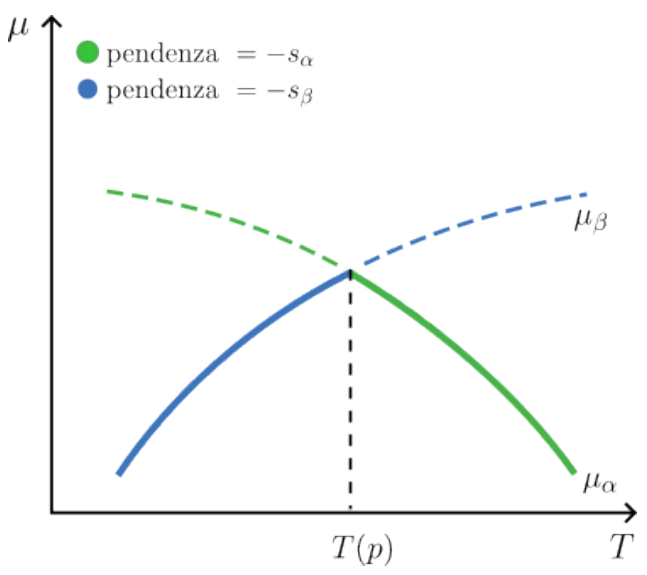
\includegraphics[width=0.4\linewidth]{Immagini/transizione I ordine p costante.png}
    \caption{transizione del primo ordine a pressione $p$ costante.}
    \label{fig: transizione I ordine p costante}
\end{figure}

Quindi, in generale alla transizione $S_\alpha \neq S_\beta$. In particolare, nell'esempio di sistema raffigurato in figura \ref{fig: transizione I ordine p costante}, si ha $S_\alpha > S_\beta$. Per $T = T(p) - \epsilon$, ossia subito prima della transizione, il sistema è nella fase $\beta$ per cui $S_{(-)} = NS_\beta$, invece per $T = T(p) + \epsilon$ il sistema è nella fase $\alpha$ per cui adesso $S_{(+)} = NS_\alpha$, dunque
\begin{equation}
    \Delta S = S_{(+)} - S_{(-)} = N(S_\alpha - S_\beta) > 0,
\end{equation}
cioè durante la transizione si ha un aumento di entropia e di conseguenza un calore latente $L$ dato da $L = T\Delta S$. Tale calore latente corrisponde anche alla variazione di entalpia del sistema, infatti se in
\begin{equation}
    H(S,p,N) = G(T,p,N) + TS
\end{equation}
si sostituisce la condizione di equilibrio $\mu_\alpha = \mu_\beta$, ossia $\Delta G = 0$, si ha
\begin{equation}
    \Delta H = \Delta(TS) = T\Delta S = L.
\end{equation}
Mantenendo invece costante la temperatura, la situazione tipica risulta essere simile a quella raffigurata in figura \ref{fig: transizione I ordine T costante}.
\begin{figure}[h]
    \centering
    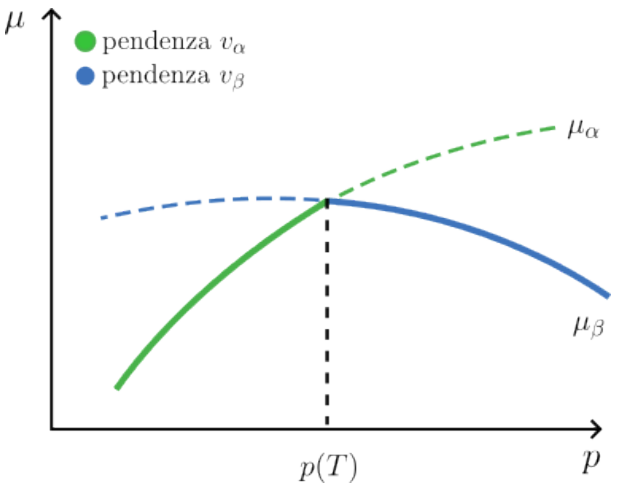
\includegraphics[width=0.4\linewidth]{Immagini/transizione I ordine T costante.png}
    \caption{transizione del primo ordine a temperatura $T$ costante.}
    \label{fig: transizione I ordine T costante}
\end{figure}

In generale, la derivata $\p_p\mu|_{T,N}$ è discontinua alla transizione. Siccome $\mu = G/N$ e $\p_pG|_{T,N} = V$ si ha, in una fase $\alpha$, che
\begin{equation}
    \frac{\p\mu_\alpha}{\p p}\bigg|_{T,N} = \frac{V_\alpha}{N_\alpha} = v_\alpha.
\end{equation}
Quindi, in generale alla transizione $v_\alpha \neq v_\beta$. In particolare, nell'esempio di sistema raffigurato in figura \ref{fig: transizione I ordine T costante}, si ha $v_\alpha > v_\beta$. Per $p = p(T) - \epsilon$, ossia subito prima della transizione, tutte le particelle sono nella fase $\alpha$ per cui $V_{(-)} = Nv_\alpha$, invece per $p = p(T) + \epsilon$ tutte le particelle sono nella fase $\beta$ per cui $V_{(+)} = Nv_\beta$, dunque
\begin{equation}
    \Delta V = V_{(+)} - V_{(-)} = N(v_\beta - v_\alpha) < 0.
\end{equation}
Quindi, se nella transizione si ha una discontinuità in
\begin{equation}
    \frac{\p\mu}{\p T}\bigg|_{p,N}\Longleftrightarrow\Delta S = \frac{L}{T}
\end{equation}
eventualmente insieme ad una discontinuità in
\begin{equation}
    \frac{\p\mu}{\p p}\bigg|_{T,N}\Longleftrightarrow\Delta V,
\end{equation}
la transizione è detta del ``primo ordine''.
\paragraph{Transizioni continue.} Se anche le derivate prime di $\mu$ sono continue alla transizione allora questa viene detta ``continua''. In tal caso, nella transizione stessa non si ha variazione di entropia né di volume, ossia $\Delta S = \Delta V = 0$. Vi sono però in generale discontinuità o singolarità in altre osservabili. Ad esempio, in un sistema con un solo tipo di componenti, una transizione continua può avvenire solo in punti nel piano $(p,T)$, detti ``punti critici'', che normalmente si trovano al termine di un tratto di una curva di coesistenza per una transizione del primo ordine. Il motivo di ciò è che in realtà esiste una richiesta di continuità aggiuntiva.

\section{Equazione di Clausius - Clapeyron}
Ci si chiede adesso come sia possibile determinare esplicitamente la curva di coesistenza $p(T)$ per una transizione del primo ordine. Per rispondere a ciò, si determina prima l'espressione per $dp/dT$ che poi, normalmente sotto qualche tipo di ipotesi semplificante, può essere integrata. Quindi, ricordando sempre che $\mu = G/N$ e che 
\begin{equation}
    d\mu = -sdT +vdp,\quad s = \frac{S}{N},\,v = \frac{V}{N},
\end{equation}
lungo la curva di coesistenza si ha $\mu_\alpha = \mu_\beta$, per cui spostandosi lungo essa di un tratto infinitesimo si ha $d\mu_\alpha = d\mu_\beta$, sostituendo ora l'espressione di $d\mu$ si ottiene
\begin{equation}
\label{eq: dp/dT per eq. CC}
    -s_\alpha dT + v_\alpha dp = -s_\beta dT + v_\beta dp,
\end{equation}
da cui, si ricava l'equazione di Clausius-Clapeyron
\begin{equation}
    \frac{dp}{dT} = \frac{\Delta S}{\Delta V},
\end{equation}
che può essere riscritta usando la relazione tra variazione di entropia e calore latente come
\begin{equation}
\label{eq: dp/dT per eq. CC in funzione di L}
    \frac{dp}{dT} = \frac{L}{T\Delta V} = \frac{l}{T\Delta v},\quad l =\frac{L}{N}.
\end{equation}
Siccome il membro di destra della \eqref{eq: dp/dT per eq. CC in funzione di L} è un rapporto, lo si può anche esprimere in termini del calore latente molare $l_{mol}$ e del volume molare $v_{mol}$ definiti come
\begin{equation}
    l_{mol} = \frac{L}{n_{mol}} = N_Al,\quad v_{mol} = \frac{V}{n_{mol}} = N_Av,
\end{equation}
oppure in termini del calore latente specifico $l_{spec}$ e del volume specifico $v_{spec}$, ossia riferiti all'unità di massa, definiti come
\begin{align}
    l_{spec} &= \frac{L}{M} = \frac{L}{n_{mol}m_{mol}} = \frac{l_{mol}}{m_{mol}}, \\
    v_{spec} &= \frac{V}{M} = \frac{V}{n_{mol}m_{mol}} = \frac{v_{mol}}{m_{mol}},
\end{align}
ottenendo dunque
\begin{equation}
    \frac{dp}{dT} = \frac{l_{mol}}{T\Delta v_{mol}} = \frac{l_{spec}}{T\Delta v_{spec}}.
\end{equation}

\subsubsection{Tensione di vapore saturo}
Come applicazione della relazione di Clausius - Clapeyron, si considera una transizione del primo ordine da liquido a gas, precisamente vapore. Quando le due fasi coesistono, e il vapore si dice ``saturo'', $p$ e $T$ sono sulla curva di coesistenza e vale l'equazione di Clausius - Clapeyron. Aumentando $T$ si passa dalla fase liquida o quella gassosa, il calore latente è positivo e per i volumi specifici si ha
\begin{equation}
    v_{gas} \gg v_{liquido}\quad\Rightarrow\quad \Delta v \sim \Delta v_{gas}.
\end{equation}
Dunque, l'equazione \eqref{eq: dp/dT per eq. CC in funzione di L} diventa
\begin{equation}
    \frac{dp}{dT} = \frac{l}{T\Delta v_{gas}}.
\end{equation}
Ipotizzando che il gas soddisfi l'equazione di stato dei gasi ideali $pv_{gas} = kT$ si ha
\begin{equation}
    \frac{dp}{dT} = \frac{lp}{kT^2}
\end{equation}
e supponendo anche che il calore latente sia costante lungo l'intero intervallo di temperatura considerato, si può integrare l'equazione trovata ora a variabili separabili ottenendo
\begin{equation}
    p(T) = p_0\exp{\bigg[-\frac{l}{k}\bigg(\frac{1}{T} - \frac{1}{T_0}\bigg)\bigg]}.
\end{equation}
Dunque, la pressione di vapore saturo cresce molto rapidamente in funzione della temperatura.

\section{Diagramma di fase nel piano (\textit{p,V})}
Considerando un sistema che esibisca una linea di transizione di fase del primo ordine nel piano $(p,T)$ ci si chiede ora come appaia tale diagramma di fase utilizzando invece le variabili coniugate $(p,V)$ per descrivere il sistema
\begin{figure}[h]
    \centering
    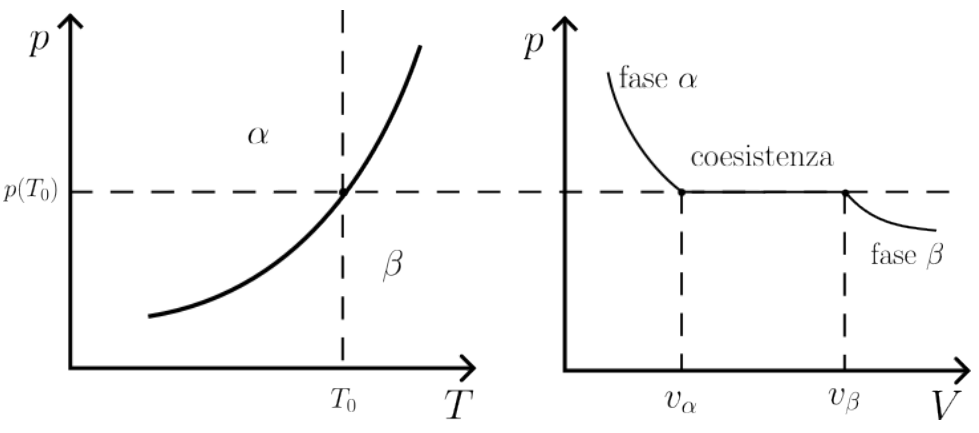
\includegraphics[width=0.6\linewidth]{Immagini/diagrammi p,T e p,V 1.png}
    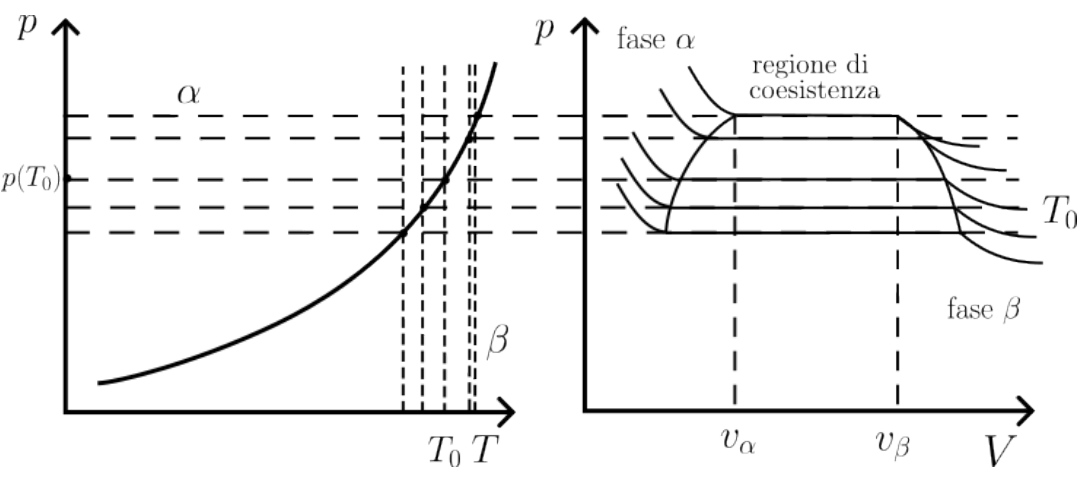
\includegraphics[width=0.6\linewidth]{Immagini/diagrammi p,T e p,V 2.png}
    \caption{relazione tra i piani $(p,T)$ e $(p,V)$.}
    \label{fig: diagrammi p,T e p,V}
\end{figure}
Facendo riferimento alla figura \ref{fig: diagrammi p,T e p,V}, il punto di transizione $(p(T_0),T_0)$ considerato diviene un segmento. Se si considerano le varie possibili isoterme si osserva che la singola curva di coesistenza diventa un'intera regione di coesistenza, dove si ricorda che la stabilità dello stato di equilibrio impone che
\begin{equation}
    \frac{\p p}{\p V}\bigg|_{T,N} \le 0,
\end{equation}
condizione soddisfatta dalle isoterme in figura \ref{fig: diagrammi p,T e p,V}. Adesso, si considera nuovamente un'isoterma fissata mostrata sempre in figura \ref{fig: diagrammi p,T e p,V}. Lungo il segmento orizzontale vi sono stati che differiscono per il numero di particelle $N_\alpha$ che sono nella fase $\alpha$ e quelli che sono nella fase $\beta$, il cui volume è
\begin{equation}
    V = N_\alpha v_\alpha + N_\beta v_\beta,\quad N_\beta = 1 - N_\alpha,
\end{equation}
che diviso per $N$, definendo $\nu_{\alpha,\beta} = N_{\alpha,\beta}/N$ restituisce il volume per particella 
\begin{equation}
\label{eq: volume spcifico}
    v = \nu_\alpha v_\alpha + \nu_\beta v_\beta,\quad \nu_\beta = 1 - \nu_\alpha.
\end{equation}
Da ciò seguono le relazioni
\begin{align}
    v - v_\alpha &= (\nu_\alpha - 1)v_\alpha + \nu_\beta v_\beta = -\nu_\beta v_\alpha + \nu_\beta v_\beta = \nu_\beta(v_\beta - v_\alpha), \\
    v_\beta - v &= -\nu_\alpha v_\alpha + (1 - \nu_\beta)v_\beta = -\nu_\alpha v_\alpha + \nu_\alpha v_\beta = \nu_\alpha(v_\beta - v_\alpha),
\end{align}
che divise membro a membro restituiscono la cosiddetta ``regola della leva''
\begin{equation}
\label{eq: regola della leva}
    \frac{\nu_\beta}{\nu_\alpha} = \frac{v - v_\alpha}{v_\beta - v}.
\end{equation}
I volumi specifici $v_\alpha$ e $v_\beta$ che determinano gli estremi del segmento di coesistenza nel grafico $p(v)$ ad una temperatura fissata $T$ sono implicitamente determinati dalle due condizioni
\begin{equation}
    \begin{cases}
        p_\alpha(T,v_\alpha) = p_\beta(T,v_\beta) = p(T) \\
        \mu_\alpha(T,v_\alpha) = \mu_\beta(T,v_\beta)
    \end{cases}.
\end{equation}
Di queste due condizioni si considera un'interpretazione geometrica in termini dell'energia libera di per particella $f = F/N$, l'energia libera di Helmoltz $F(T,V,N)$ in effetti è il potenziale rilevante quando le variabili indipendenti sono $T$, $V$ ed $N$. Siccome $p$ è data da
\begin{equation}
    -p = \frac{\p f}{\p v}\bigg|_{T,N},
\end{equation}
allora si può dedurre dal grafico di $p(v)$ quello di $f(v)$ per un valore di $T$ fissato. 
\begin{figure}[h]
    \centering
    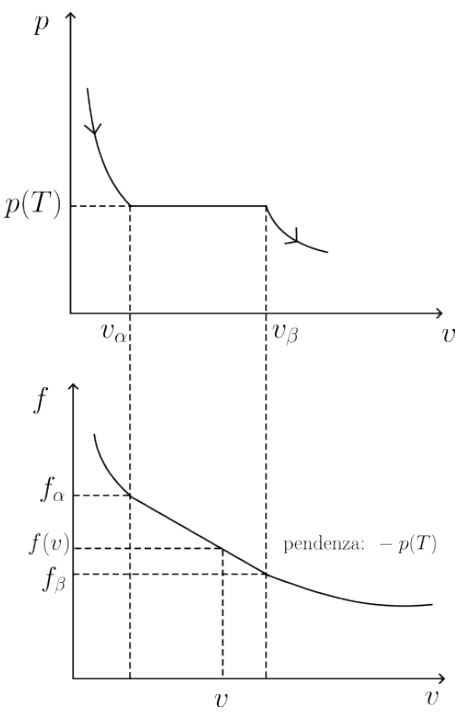
\includegraphics[width=0.45\linewidth]{Immagini/relazione digrammi p,v e f,v.png}
    \caption{relazione tra i piani $(p,v)$ e $(f,v)$.}
    \label{fig: relazione digrammi p,v e f,v}
\end{figure}

Ad esempio, si consideri il segmento rettilineo nel grafico \ref{fig: relazione digrammi p,v e f,v}, in questo caso si ha
\begin{equation}
    \begin{split}
        \frac{f_\beta - f_\alpha}{v_\beta - v_\alpha} &= -p \\
        f_\beta - f_\alpha &= -p(v_\beta - v_\alpha) \\
        (f + pv)_\beta &= (f + pv)_\alpha.
    \end{split}
\end{equation}
A causa della trasformata di Legendre che lega $F$ e $G$, $f + pv$ è l'energia di Gibbs specifica
\begin{equation}
    \mu = f + pv.
\end{equation}
Dunque, si è ritrovata la condizione $\mu_\alpha = \mu_\beta$. Per un generico $v\in[v_\alpha,v_\beta]$, come visto precedentemente, si ha $v = \nu_\alpha v_\alpha + \nu_\beta v_\beta$ quindi il valore di $f(v)$ desumibile dal grafico \ref{fig: relazione digrammi p,v e f,v}, cioè dalla proporzione
\begin{equation}
    \frac{f(v) - f_\alpha}{v - v_\alpha} = \frac{f_\beta - f_\alpha}{v_\beta - v_\alpha},
\end{equation}
che usando la relazione \eqref{eq: volume spcifico} diventa
\begin{equation}
    f = \nu_\alpha f_\alpha + \nu_\beta f_\beta.
\end{equation}

\section{Costruzione di Maxwell}
Si supponga di conoscere una descrizione approssimata di un certo sistema tramite un'equazione di stato $p \equiv p(T,V)$ che però, in alcune regioni, viola il criterio di stabilità, come ad esempio il caso del grafico in figura \ref{fig: costruzione di Maxwell}. In particolare, nella regione delimitata si ha la violazione
\begin{equation}
    \frac{\p p}{\p V}\bigg|_{T,N} > 0 \quad\Rightarrow\quad \kappa_T < 0.
\end{equation}
L'obiettivo quindi è rimpiazzare la curva contenuta nella regione compromessa con un'altra curva tale che:
\begin{enumerate}
    \item l'instabilità sia rimpiazzata da una transizione di fase del primo ordine che avviene ad una certa pressione $\bar{p}$;
    \item al di fuori della transizione l'equazione di stato rimanga quella graficata in figura \ref{fig: costruzione di Maxwell}.
\end{enumerate}
\begin{figure}[h]
    \centering
    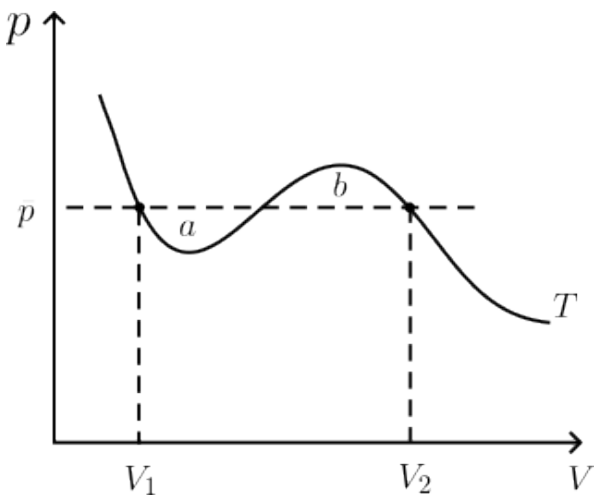
\includegraphics[width=0.4\linewidth]{Immagini/costruzione di Maxwell.png}
    \caption{costruzione di Maxwell per equazioni di stato violanti il criterio di stabilità.}
    \label{fig: costruzione di Maxwell}
\end{figure}

Essenzialmente, si vuole determinare il tratto orizzontale rappresentato in \ref{fig: costruzione di Maxwell} in modo che l'energia libera in $V_1$ e in $V_2$ coincida con quella prevista dall'equazione di stato approssimata. Siccome, l'energia libera $dF$ è data da
\begin{equation}
    dF = -SdT - pdV + \mu dN,
\end{equation}
ad $N$ e $T$ fissati si ha $dN = 0$ e $dT = 0$, per cui
\begin{equation}
    F(V_2,T,N) - F(V_1,T,N) = -\int_{V_1}^{V_2} p(V,T,N)\,dV.
\end{equation}
Se quest'ultimo integrale deve coincidere con la curva originale e per il segmento orizzontale, devono essere uguali le aree sottostanti. Quindi, $V_1$ e $V_2$ vanno determinati in modo che 
\begin{equation}
    \bar{p}(V_2 - V_1) = \int_{V_1}^{V_2} p(V,T)\,dV,
\end{equation}
dove $p(V,T)$ è la curva approssimata originale. In altri termini, le due aree indicate come $A$ e $B$ in figura \ref{fig: costruzione di Maxwell} devono risultare uguali. 

\subsection{Equazione di stato di Van der Waals}
L'equazione di stato di Van der Waals è un primo esempio di tentativo alla descrizione fenomenologica delle interazioni molecolari tra le componenti di un gas. Tipicamente, il potenziale intermolecolare ha una funzione del tipo graficato in figura \ref{fig: potenziale Van der Waals}. 
\begin{figure}[h]
    \centering
    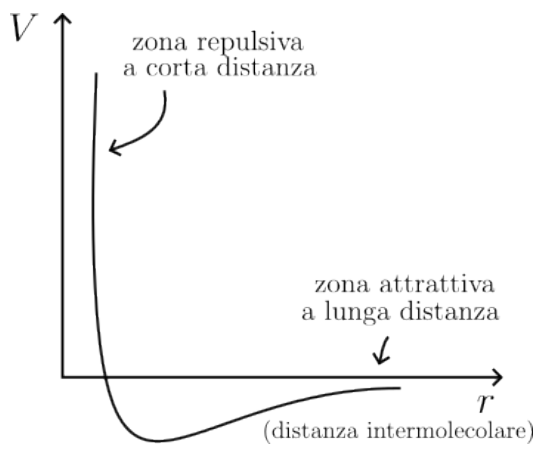
\includegraphics[width=0.4\linewidth]{Immagini/potenziale Van der Waals.png}
    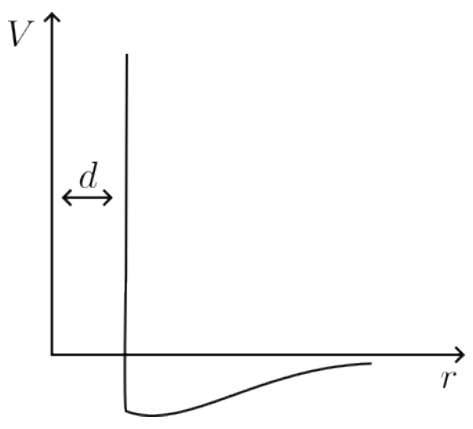
\includegraphics[width=0.36\linewidth]{Immagini/potenziale Van der Waals hardcore.png}
    \caption{(i) forma tipica del potenziale di interazione intermolecolare; (ii) approssimazione ``hardcore''.}
    \label{fig: potenziale Van der Waals}
\end{figure}

Il modello di Van der Waals descrive la regione repulsiva del potenziale tramite un ``hardcore'', ossia considerando le particelle come sfere indeformabili di un certo raggio, la conseguenza principale è che il volume effettivamente a disposizione delle molecole viene ridotto ad un volume efficace 
\begin{equation}
\label{eq: volume efficace Van der Waals}
    V_{eff} = V - b,\quad b\in\R
\end{equation}
dove $b$ è una costante che dipende unicamente dalla sostanza che compone il gas. La presenza di una parte attrattiva del potenziale implica la tendenza del sistema a formare stati legati. Questo comporta una diminuzione della pressione proporzionale al numero di coppie di molecole in uno stato vicino alle pareti. Questo effetto, è proporzionale al quadrato della densità $(N/V)^2$, quindi da
\begin{equation}
    \Delta p \propto n_{coppie} \propto \bigg(\frac{N}{V}\bigg)^2.
\end{equation}
L'ipotesi di Van der Waals è
\begin{equation}
\label{eq: I ipotesi Van der Waals}
    p = p_K - \frac{a}{V^2},
\end{equation}
dove $p_K$ è la pressione in assenza di interazioni ed è un'altra costante dipendente unicamente dalla sostanza in esame. Una ulteriore ipotesi è quella che $p_K$ soddisfi l'equazione di stato dei gas perfetti
\begin{equation}
\label{eq: II ipotesi Van der Waals}
    p_KV_{eff} = nRT.
\end{equation}
\begin{notz}
    D'ora in poi si considera il numero di moli $n$ pari a $n = 1$ in modo da non doverlo includere in ogni passaggio.
\end{notz}
Dunque, sostituendo le relazioni \eqref{eq: volume efficace Van der Waals} e \eqref{eq: I ipotesi Van der Waals} in \eqref{eq: II ipotesi Van der Waals} si ottiene l'equazione di stato di Van der Waals
\begin{equation}
\label{eq: equazione di stato Van der Waals}
    \bigg(p + \frac{a}{V^2}\bigg)(V - b) = RT.
\end{equation}
L'equazione \eqref{eq: equazione di stato Van der Waals} nel limite $V\to\infty$ si riduce all'equazione di stato classica dei gas perfetti $pV = RT$. In generale, l'equazione di Van der Waals è un polinomio di terzo grado in $V$, per cui un generico grafico delle isoterme è tipicamente del tipo rappresentato in figura \ref{fig: isoterme Van der Waals}. 
\begin{figure}[h]
    \centering
    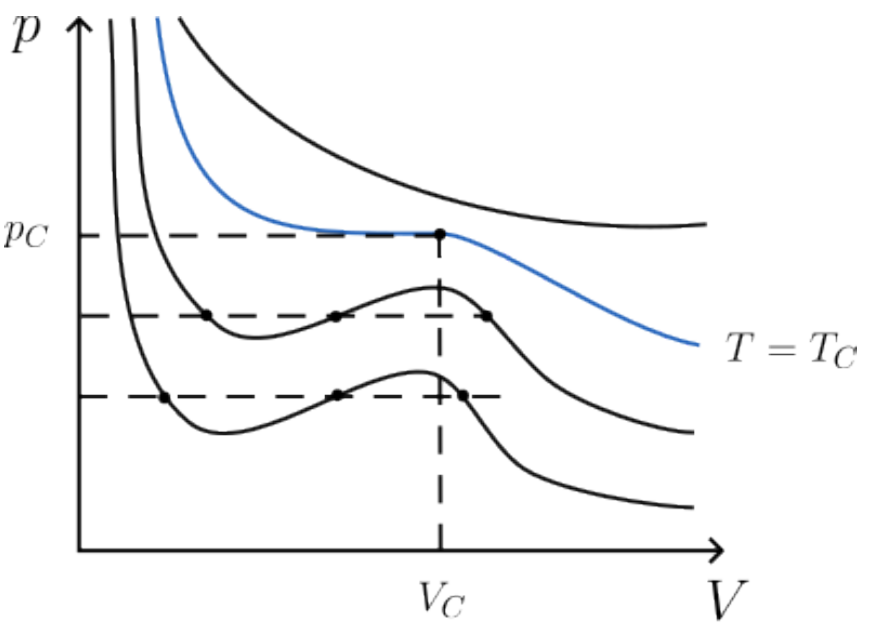
\includegraphics[width=0.42\linewidth]{Immagini/isoterme Van der Waals.png}
    \caption{grafico delle isoterme nel piano $(p,V)$ per l'equazione di Van der Waals.}
    \label{fig: isoterme Van der Waals}
\end{figure}

Tuttavia, al di sotto di una certa temperatura critica $T_C$ si nota che sarebbe comunque necessario usare la costruzione di Maxwell per correggere le previsioni dell'equazione \eqref{eq: equazione di stato Van der Waals}, la quale infatti trascura la possibilità di transizioni in cui il sistema si separa in due fasi. 
\begin{obs}
    L'equazione \eqref{eq: equazione di stato Van der Waals} si può parametrizzare invece che in termini di $a$ e $b$ che dipendono dalla sostanza in questione, in termini dei valori critici di pressione $p_C$, temperatura $T_C$ e volume $V_C$ indipendenti da essa. Definendo allora le variabili ridotte
    \begin{equation}
        \bar{p} = \frac{p}{p_C},\quad \bar{T} = \frac{T}{T_C},\quad \bar{V} = \frac{V}{V_C},
    \end{equation}
    si può esprimere l'equazione di stato di Van der Waals, dopo una serie di passaggi, come la ``legge degli stati corrispondenti'' 
    \begin{equation}
        \bigg(\bar{p} + \frac{3}{\bar{V}^2}\bigg)\bigg(\bar{V} - \frac{1}{3}\bigg) = \frac{8}{3}\bar{T}.
    \end{equation}
\end{obs}

\section{Coesistenza multifase}
Si considera una sistema con una singola componente che presenta al più tre fasi $\alpha$, $\beta$ e $\gamma$. La richiesta affinché queste fasi coesistano è
\begin{equation}
    \mu_\alpha(T,p) = \mu_\beta(T,p) = \mu_\gamma(T,p),
\end{equation}
che può essere ripartita in due equazioni indipendenti da $p$ e $T$
\begin{equation}
    \begin{cases}
        \mu_\alpha(T,p) = \mu_\gamma(T,p) \\
        \mu_\beta(T,p) = \mu_\gamma(T,p)
    \end{cases},
\end{equation}
la cui soluzione può essere un singolo punto o un insieme di punti. Un esempio, può essere il primo in figura \ref{fig: esempi di diagrammi di fase}, dove sono presenti due punti di coesistenza delle tre fasi, oppure il secondo sempre in figura \ref{fig: esempi di diagrammi di fase}, dove è presente un unico punto di coesistenza come accade per il diagramma di fase dell'acqua. 
\begin{figure}[h]
    \centering
    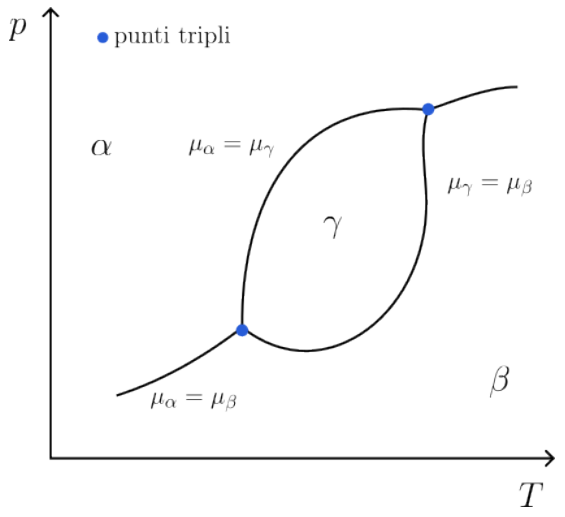
\includegraphics[width=0.4\linewidth]{Immagini/diagramma di fase (2 p.ti critici).png}
    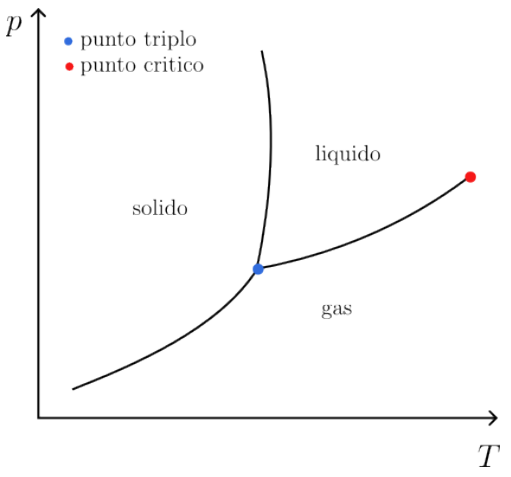
\includegraphics[width=0.39\linewidth]{Immagini/diagramma di fase (1 p.to critici).png}
    \caption{(ii) diagramma di fase fittizio con due punti critici; (ii) diagramma di fase dell'acqua.}
    \label{fig: esempi di diagrammi di fase}
\end{figure}

I punti di coesistenza vengono tipicamente chiamati ``punti tripli'', mentre agli estremi delle linee di transizione di fase possono essere presenti dei ``punti critici'' $C$. La presenza di tali punti critici, come nel caso dell'acqua, corrisponde, dal punto di vista qualitativo, che la fase liquida e la fase gassosa differiscono solo per un minore o un maggiore grado di interazione molecolare, permettendo di pensare di poter passare da uno all'altro senza dover passare da una linea di transizione. In altre parole, le transizioni oltre il punto critico le isoterme non presentano più alcuna transizione di fase del primo ordine e quindi le transizioni risultano essere continue, in particolare si ha $\Delta V = 0$. In pratica, si possono realmente distinguere le due fasi solo quando esistono contemporaneamente, cioè lungo la curva di coesistenza. 
\begin{obs}
    Ovviamente, un diagramma di fase può essere graficato su un piano differenze, ad esempio quello dell'acqua in figura \ref{fig: esempi di diagrammi di fase} sul piano $(p,T)$ può essere riportato invece su un piano $(p,V)$ come mostrato in figura \ref{fig: diagramma di fase acqua (p,V)}.
    \begin{figure}[h]
        \centering
        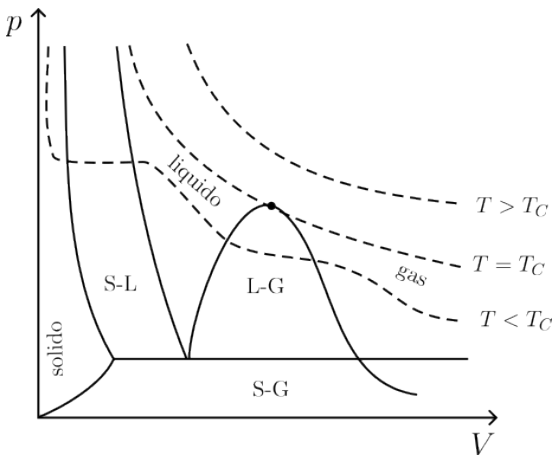
\includegraphics[width=0.4\linewidth]{Immagini/diagramma di fase acqua (p,V).png}
        \caption{diagramma di fase dell'acqua nel piano $(p,V)$.}
        \label{fig: diagramma di fase acqua (p,V)}
    \end{figure}
\end{obs}

\subsection{Sistemi multicomponenti}
Si supponga adesso di avere un sistema composto da una miscela di un certo numero $C$ di componenti macroscopiche diverse e che questo si trovi in una situazione di equilibrio in cui coesistono un certo numero $f$ di fasi. Si denota con $\nu_{i,a}$, con $i = 1,\dots,C$ e $\alpha=1,\dots,f$, la frazione di particelle dell'$i$-esimo tipo che si trovano nell'$\alpha$-esima fase, con la condizione che tali fasi debbano soddisfare il vincolo
\begin{equation}
    \nsum_i\nu_{i,\alpha} = 1,\quad\forall\alpha.
\end{equation}
Esistono quindi $(C - 1)$ variabili indipendenti per ogni $\alpha$, per un totale di $f(C - 1)$ variabili indipendenti. La condizione di coesistenza sono la costanza della coppia di variabili $(p,T)$ in tutte le fasi e l'uguaglianza dei potenziali chimici $\mu_{i,\alpha}$. Quindi, si hanno $C(f - 1)$ equazioni in $2 + f(C - 1)$ variabili
\begin{equation}
    \mu_{i,1}(p,T,\nu_{1,1},\dots,\nu_{C - 1,1}) = \cdots = \mu_{i,f}(p,T,\nu_{1,f},\dots,\nu_{C - 1,f}),\quad\forall i.
\end{equation}
Tutto ciò può essere interpretato come la coesistenza su una ipersuperficie parametrizzata da $2 + f(C - 1) - C(f - 1) = 2 + C - f$ variabili indipendenti. Dunque, il numero massimo di fasi $f$ coesistenti per un dato sistema di $C$ componenti è dato da
\begin{equation}
    f = 2 + C.
\end{equation}
\chapter{Meccanica statistica}
I sistemi macroscopici oggetto dello studio della Termodinamica sono tipicamente costituiti da un numero molto elevato $N$ di componenti macroscopiche variamente interagenti dell'ordine del numero di Avogadro $N_A \simeq 6\times 10^{23}$. Microscopicamente, gli stati $\nu$ del sistema sono caratterizzati da un numero enorme, almeno di ordine $N$, di numeri quantici, o quando l'approssimazione classica è applicabile, di coordinate nello spazio delle fasi. Si supponga, per fissare le idee, che i componenti microscopici di un sistema possano essere trattati come particelle classiche puntiformi. In tal caso, uno stato microscopico, ossia un ``microstato'', è caratterizzato da $2\cdot3N = 6N$ coordinate nello spazio delle fasi delle $N$ particelle
\begin{equation}
    \nu_i \longleftrightarrow (\vq_i,\vp_i) = (q^\alpha_i,p_{\alpha,i}) = (q^A,p_A),
\end{equation}
dove $i = 1,\dots,N$, $\alpha=1,2,3$ e quindi $A = (i,\alpha) = 1,\dots,6N$. Se si considera un sistema quantistico di $N$ oscillatori armonici tridimensionali disaccoppiati, o debolmente accoppiati, una base di microstati è caratterizzata tramite i numeri quantici $\vn_i = n_{i,\alpha}$ degli $N$ oscillatori. Uno stato generico quindi è
\begin{equation}
    \ket{\nu(t)} = \sum_{\{\vn_i\}} c(\{\vn_i\},t)\ket{\vn_1,\dots,\vn_N}.
\end{equation}
L'evoluzione di un microstato $\nu(t)$ è determinata dalle equazioni della dinamica classica o quantistica a seconda del contesto. Nel primo caso, se l'hamiltoniana del sistema è $H(q^A,p_A)$, la dinamica è descritta dalle equazioni di Hamilton
\begin{equation}
\label{eq: equazioni di Hamilton}
    \begin{cases}
        \dot{q}^A = \dfrac{\p H}{\p p_A} \\[2ex]
        \dot{p}_A = -\dfrac{\p H}{\p q^A}
    \end{cases},\quad A = 1,\dots,6N.
\end{equation}
Tramite le equazioni \eqref{eq: equazioni di Hamilton} e la conoscenza esatta di $6N$ condizioni iniziali $\{q^A(0),p_A(0)\}$ si può determinare univocamente la traiettoria nello spazio delle fasi che non si autointerseca mai.
\begin{notz}
    In alcune situazioni si può anche usare una notazione vettoriale delle equazioni \eqref{eq: equazioni di Hamilton}
    \begin{equation}
        \begin{cases}
        \dot{\vq}_i = \dfrac{\p H}{\p \vp_i} \\[2ex]
        \dot{\vp}_i = -\dfrac{\p H}{\p \vq_i}
    \end{cases},\quad i = 1,\dots,N.
    \end{equation}
\end{notz}
L'evoluzione dinamica secondo la trattazione classica presenta delle caratteristiche importanti che sono problematiche riguardo all'accordo con la descrizione macroscopica termodinamica. Si mostrano le principali incongruenze.

\paragraph{Reversibilità temporale.} Se il sistema può evolvere lungo una certa traiettoria nello spazio delle fasi, allora anche l'evoluzione inversa è possibile. Quindi, se il sistema evolve dalla situazione iniziale $\{\vq_i(0),\vp_i(0)\}$ allo stato finale $\{\vq_i(t_1),\vp_i(t_1)\}$, allora effettuando l'inversione temporale $t\to t_1 - t'$, si ottiene l'evoluzione inversa dallo stato $\{\vq_i(t'=0),\vp_i(t'=0)\}$ allo stato $\{\vq_i(t'=t_1),\vp_i(t'=t_1)\}$, come mostrato in figura \ref{fig: reversibilità temporale (teo. H)}. Il problema con questa affermazione riguardava la formulazione del teorema H di Boltzmann e il fatto che questo selezionasse una direzione temporale preferenziale, appunto inconsistente con l'invarianza del sistema sotto inversione temporale. Tuttavia, l'incongruenza era solo apparente in quanto l'assunzione su cui si basa è falsa: l'invarianza per inversione temporale non è inconsistente con il teorema H in quanto non è necessario che $\dot{H}$ sia una funzione continua nel tempo. Una spiegazione più chiara di quanto detto verrà esposta in seguito alla derivazione del teorema H.
\begin{figure}[h]
    \centering
    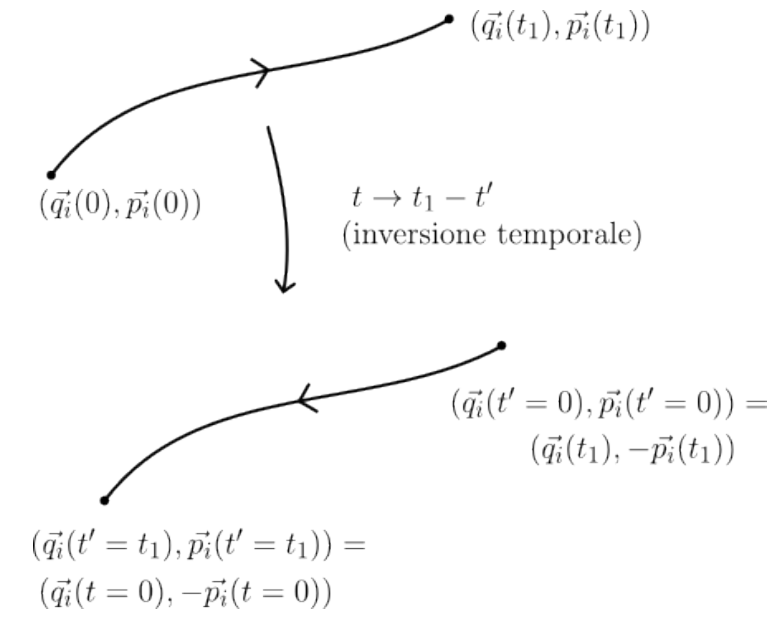
\includegraphics[width=0.5\linewidth]{Immagini/reversibilità temporale (teo. H).png}
    \caption{reversibilità temporale di un sistema.}
    \label{fig: reversibilità temporale (teo. H)}
\end{figure}

\paragraph{Cicli di Poincaré.} Si supponga che il moto del sistema nello spazio delle fasi sia confinato in una regione limitata. Questa richiesta è praticamente sempre verificata in quanto il volume spaziale in cui le componenti di un sistema reale si possono muovere è finito e i momenti non possono tendere all'infinito a causa delle restrizioni imposte dalla Relatività speciale. Si può allora dimostrare che la traiettoria nello spazio delle fasi ripasserà arbitrariamente vicino ad ognuno dei suoi punti, per un generico stato iniziale, dopo un tempo sufficientemente lungo ed escludendo solamente l'insieme degli stati a misura nulla.

\section{Approccio statistico}
Per sistemi microscopici con un numero elevato $N$ di componenti, è di fatto impensabile descriverli classicamente a causa della ridondanza delle $O(N)$ variabili microscopiche. Il comportamento macroscopico all'equilibrio è invece efficacemente descritto tramite poche variabili macroscopiche termodinamiche. Il comportamento del sistema è quindi prevedibile usando i principi della Termodinamica e le particolari equazioni di stato del sistema stesso. In Termodinamica le equazioni di stato dei sistemi sono descritte sperimentalmente. In Meccanica statistica, invece si intende utilizzare la conoscenza della struttura microscopica del sistema per dedurre le equazioni di stato dello stesso. Quando il sistema in equilibrio è caratterizzato da un set di valori delle variabili termodinamiche si dice che si trova in un certo ``macrostato'' di equilibrio. Ad un dato macrostato corrisponde tipicamente un numero enorme di possibili microstati $\nu$. Ad esempio, a fissate $E$, $V$ ed $N$, le particelle di un gas diluito possono essere distribuite, in qualsiasi modo all'interno del volume $V$ e l'energia $E$ può essere distribuita in ogni modo fra di esse. Il sistema nel tempo esplora lo spazio dei possibili microstati, sia che si trovi all'equilibrio, sia che non lo sia per effetto delle interazioni fra le componenti del sistema ed eventualmente del sistema stesso, al più quasi-isolato, con l'ambiente, che ne determina l'evoluzione temporale. Nel farlo, segue una traiettoria $\nu(t)$, passando da un microstato all'altro su una scala temporale $\tau$ tipica della dinamica molecolare, in genere molto breve. In tempi $t \gg \tau$, il sistema visita i possibili microstati con una certa frequenza che all'equilibrio è stazionaria.

Si consideri ora un'osservabile $O$. Una misura affidabile $\tilde{O}$ del suo valore effettuata in un tempo $t \gg \tau$ si può pensare corrisponda alla media di $M$ osservazioni ``istantanee'', ossia svolte in tempo $t \ll \tau$, in modo tale che il sistema si trovi in un definito microstato
\begin{equation}
\label{eq: stima O tramite osservazioni}
    \tilde{O} = \frac{1}{M}\sum_{i = 1}^M \tilde{O}_i.
\end{equation}
Ci si domanda come si potrebbe predire tale risultato a partire dalla conoscenza della struttura microspica. Se fosse possibile determinare in modo esatto l'evoluzione temporale $\nu(t)$ del sistema risolvendo le equazioni di Hamilton, o di Schr\"odinger, e trovando quindi $\{q^A(t),p_A(t)\}$, allora si potrebbe valutare $\tilde{O}$ tramite la media temporale 
\begin{equation}
\label{eq: stima O tramite media temporale}
    \bar{O} = \frac{1}{T}\int_{t_0}^{t_0 + T}dt\,O[\nu(t)].
\end{equation}
Tuttavia, come già detto, questo approccio è impensabile da applicare nel limite di $N\to\infty$ ed in ogni caso risulta inefficiente e ridondante. Invece, si può rimaneggiare l'espressione \eqref{eq: stima O tramite osservazioni} contando il numero di volte $n(\nu)$ in cui appare in essa un certo microstato $\nu$, ottenendo così
\begin{equation}
\label{eq: stima O tramite probabilità (discreta)}
    \tilde{O} = \nsum_{\{\nu\}}\frac{n(\nu)}{M}O(\nu) \simeq \nsum_\nu P(\nu)O(\nu) \equiv \vmedio{O}.
\end{equation}
Infatti, nel limite $M\to\infty$, quindi per un tempo $t$ pari al tempo di misura, si ha $Mt \gg \tau$ e $n(\nu)/M$ è la definizione frequentistica della probabilità $P(\nu)$ che il sistema si trovi nel microstato $\nu$. Nel caso di un sistema classico, dove i microstati corrispondono a punti dello spazio delle fasi, l'espressione discreta \eqref{eq: stima O tramite probabilità (discreta)} passa al continuo diventando
\begin{equation}
\label{eq: stima O tramite probabilità (continua)}
    \tilde{O} \simeq \vmedio{O} = \int dq\,dp\,\rho(\{q^A,p_A\})O(\{q^A,p_A\}),
\end{equation}
dove $\rho(\{q^A,p_A\})\,dq\,dp$ corrisponde alla probabilità che il sistema sia nella porzione di spazio delle fasi compresa tra $[q,q+dq;p,p+dp]$, per cui $\rho(\{q^A,p_A\})$ è una densità di probabilità. 
\begin{notz}
    Per semplicità di notazione, nel seguito si pone $d\mu := dq\,dp$ e $(q,p) \equiv \{q^A,p_A\}$.
\end{notz}
In generale, la condizione perché uno stato sia di equilibrio è che la $\rho(q,p)$ sia stazionaria, mentre in uno stato generico diverso da uno di equilibrio ci si aspetta che $\rho(q,p)$ dipenda esplicitamente dal tempo $t$ risultando in una funzione $\rho(q,p,t)$. Tuttavia, l'evoluzione di $\rho$ è determinata dalle equazioni della Meccanica hamiltoniana microscopica: se si avesse qualche principio che conducesse a determinare $\rho$, almeno all'equilibrio, senza risolvere esplicitamente le equazioni del moto, questo permetterebbe di applicare l'approccio statistico desiderato. 

\subsection{Sottosistemi macroscopici}
Quando si descrive un sistema macroscopico, si può ancora suddividerlo in tanti sottosistemi, ancora macroscopici. Questi sistemi non sono isolati, ma interagiscono in modo continuo con le altre parti del sistema. Dato però che queste parti, piccole rispetto al sistema intero, sono anch'esse corpi macroscopici, è lecito assumere che in intervalli di tempo non troppo lunghi rispetto alla scala temporale $\tau$ della dinamica microscopica, si comportino pressappoco come sistemi isolati. Infatti, sono prevalentemente le particelle che si trovano in prossimità della superficie del sottosistema ad entrare in interazione con le parti circostanti, ma il numero relativo di queste particelle rispetto al numero totale di particelle del sottosistema diminuisce rapidamente quando le sue dimensioni aumentano; inoltre, se il sottosistema è sufficientemente grande, l'energia di interazione con le parti circostanti sarà piccola rispetto alla sua energia interna. Si può quindi affermare che i sottosistemi sono quasi-isolati. In un intervallo di tempo sufficientemente lungo invece, l'effetto dell'interazione tra i sottosistemi, debole che sia, si manifesta in ogni caso, influenzando anche l'interno del sottosistema. Infatti, è proprio questa interazione relativamente debole a permettere l'evoluzione del sottosistema verso l'equilibrio statistico. Questo è il contenuto del teorema di Liouville.
\begin{teo}[di Liouville]
\label{teo: teorema di Liouville}
    Se $\rho(q,p,t)$ è una densità di probabilità che soddisfa l'equazione di continuità, allora 
    \begin{equation}
        \frac{d\rho}{dt} = \frac{\p \rho}{\p t} + \nsum_A\bigg(\frac{\p\rho}{\p q^A}\dot{q}^A + \frac{\p\rho}{\p p_A}\dot{p}_A\bigg) = 0;
    \end{equation}
    che usando le equazioni di Hamilton \eqref{eq: equazioni di Hamilton} risulta equivalente all'equazione di Liouville
    \begin{equation}
    \label{eq: equazione di Liouville}
         \frac{d\rho}{dt} = \frac{\p\rho}{\p t} + \acomm{\rho}{H} = 0
    \end{equation}
\end{teo}
\begin{proof}
    L'equazione di continuità è in generale un'espressione della forma
    \begin{equation}
    \label{eq: equazione di continuità (dim. teo. Liouville)}
        \frac{\p \rho}{\p t} + \nabla\cdot\vj = 0,
    \end{equation}
    dove in questo caso $\rho \equiv \rho(q,p,t)$ è la densità di probabilità in questione e $\vj = (\rho\dot{q}^A,\rho\dot{p}_A)$. Inoltre, $\vj$ è una costante del moto, infatti esplicitamente l'equazione \eqref{eq: equazione di continuità (dim. teo. Liouville)} ha la forma
    \begin{equation}
    \label{eq: espressione esplicita equazione di continuità (dim. teo. Liouville)}
        0 = \frac{\p\rho}{\p t} + \frac{\p(\rho\dot{q}^A)}{\p q^A} + \frac{\p(\rho\dot{p}_A)}{\p p_A} = \frac{\p\rho}{\p t} +  \frac{\p\rho}{\p q^A}\dot{q}^A + \frac{\p\rho}{\p p_A}\dot{p}_A + \rho\bigg(\frac{\p\dot{q}^A}{\p q^A} + \frac{\p\dot{p}_A}{\p q_A}\bigg).
    \end{equation}
    Usando ora le equazioni di Hamilton \eqref{eq: equazioni di Hamilton} si trova che 
    \begin{equation}
        \frac{\p\dot{q}^A}{\p q^A} + \frac{\p\dot{p}_A}{\p q_A} = \frac{\p^2H}{\p q^A\p p_A} -\frac{\p^2H}{\p p_A\p q^A} = 0,
    \end{equation}
    per cui l'ultimo termine della \eqref{eq: espressione esplicita equazione di continuità (dim. teo. Liouville)} si annulla e l'equazione \eqref{eq: equazione di Liouville} segue.
\end{proof}
\begin{obs}
    Si può vedere il teorema di Liouville anche in un altro modo. L'equazione \eqref{eq: equazione di Liouville} corrisponde al fatto che la densità di probabilità nell'intorno di un punto dello spazio delle fasi, vista da un osservatore solidale con l'evoluzione del punto stesso, resta costante. Si può vedere $\rho(q,p,t)$ come un fluido incomprimibile, il cui elemento di volume nello spazio delle fasi viene mantenuto costante durante l'evoluzione dall'hamiltoniana. Infatti, considerando un tratto di evoluzione del sistema dallo stato inziale $(q(0),p(0))$ allo stato finale $(q(t),p(t))$, si ha che al primo ordine, per uno spostamento infinitesimo e usando le equazioni di Hamilton \eqref{eq: equazioni di Hamilton}, si può scrivere
    \begin{equation}
        \begin{cases}
            q(t) \simeq q(0) - \dfrac{\p H}{\p p}\bigg|_{(q(0),p(0))}dt \\
            p(t) \simeq p(0) - \dfrac{\p H}{\p q}\bigg|_{(q(0),p(0))}dt
        \end{cases}.
    \end{equation}
    Quindi, l'elemento di volume si trasforma con lo jacobiano secondo
    \begin{equation}
        dq(0) \wedge dp(0) \to dq(t) \wedge dp(t) = J(t)[dq(0) \wedge dp(0)],
    \end{equation}
    dove per l'appunto 
    \begin{equation}
        \begin{split}
            J(t) &= \det{
            \begin{pmatrix}
                \dfrac{\p q}{\p q(0)} & \dfrac{\p q}{\p p(0)} \\[2ex]
                \dfrac{\p p}{\p q(0)} & \dfrac{\p p}{\p p(0)}
            \end{pmatrix}} \\
            &= \det{
            \begin{pmatrix}
                1 + \dfrac{\p^2 H}{\p q(0)\p p(0)}\,dt & \dfrac{\p^2 H}{\p p(0)^2}\,dt \\[2ex]
                \dfrac{\p^2 H}{\p q(0)^2}\,dt & 1 - \dfrac{\p^2 H}{\p p(0)\p q(0)}\,dt
            \end{pmatrix}} \\
            &\simeq 1 + \bigg(\dfrac{\p^2 H}{\p q(0)\p p(0)} - \dfrac{\p^2 H}{\p q(0)\p p(0)}\bigg)\,dt = 1.
        \end{split}
    \end{equation}
\end{obs}
L'assunzione che l'interazione tra i diversi sottosistemi sia debole permette anche di considerare questi sottosistemi statisticamente indipendenti, per cui lo stato in cui si trova uno dei sottosistemi non influenza in alcun modo sulle probabilità che gli altri sottosistemi si trovino in diversi stati. In termini matematici, questa proprietà si traduce nel fatto che la distribuzione statistica $\rho$ del sottosistema composto da due sottosistemi sia uguale al prodotto delle rispettive funzioni di distribuzioni dei sottosistemi componenti $\rho_1$ e $\rho_2$, ossia $\rho \equiv \rho_{12} = \rho_1\rho_2$. In generale, per un sistema composto da $N$ sottosistemi ognuno caratterizzato da una densità di probabilità $\rho_i$, con $i=1,\dots,N$, si ha che la densità di probabilità complessiva del sistema è
\begin{equation}
\label{eq: ipotesi indipendenza statistica}
    \rho \equiv \rho_{1,\dots,N} = \prod_{i = 1}^N\rho_i.
\end{equation}
A partire da questa assunzione, si consideri nuovamente un'osservabile $O_i$, questa volta relativa al solo sottosistema $i$-esimo. L'indipendenza statistica \eqref{eq: ipotesi indipendenza statistica} implica, considerando un secondo sottosistema $j$, che
\begin{equation}
    \vmedio{O_iO_j} = \vmedio{O_i}\vmedio{O_j};
\end{equation}
infatti è immediato vedere che
\begin{equation}
    \vmedio{O_iO_j} = \int d\mu_i\,d\mu_j\,\rho_{ij}O_iO_j = \int d\mu_i\,\rho_iO_i\int d\mu_j\,\rho_jO_j = \vmedio{O_i}\vmedio{O_j}.
\end{equation}
Si consideri adesso un'osservabile additiva $O$, ossia tale che
\begin{equation}
    \vmedio{O} = \sum_{i = 1}^N\vmedio{O_i} \propto N.
\end{equation}
Dato che l'osservabile $O_i$ varia nel tempo, oscillando intorno al suo valore medio, si introduce la varianza $\sigma^2$, o fluttuazione quadratica media, che caratterizza in media la larghezza dell'intervallo di tale fluttuazione, data da
\begin{equation}
\label{eq: varianza O}
    \begin{split}
        \sigma^2_O &= \vmedio{O^2} - \vmedio{O}^2 \\
        &= \bigvmedio{\bigg(\nsum_iO_i\bigg)^2} - \bigg(\nsum_i\vmedio{O_i}\bigg)^2 \\
        &= \bigvmedio{\nsum_i\nsum_jO_iO_j} - \nsum_i\nsum_j\vmedio{O_i}\vmedio{O_j} \\
        &= \nsum_i(\vmedio{O_i^2} - \vmedio{O_i}^2) + \nsum_{i\neq j}(\vmedio{O_iO_j} - \vmedio{O_i}\vmedio{O_j}) \\
        &= \nsum_i\sigma^2_i,
    \end{split}
\end{equation}
dove nel penultimo passaggio il secondo termine è nulla per l'ipotesi di indipendenza statistica \eqref{eq: ipotesi indipendenza statistica}, mentre li primo coincide proprio con la definizione di varianza per l'osservabile $O_i$ relativa all'$i$-esimo sottosistema. Dal risultato in \eqref{eq: varianza O} si deduce che $\sigma^2_O \propto N$, per cui la fluttuazione è inversamente proporzionale alla radice di $N$
\begin{equation}
    \frac{\sigma_O}{\vmedio{O}} \propto \frac{\sqrt{N}}{N} = \frac{1}{\sqrt{N}}.
\end{equation}
Le fluttuazioni relative delle osservabili additive rispetto ai loro valori medi sono piccolissime nel limite $N\to\infty$. Perciò, per un numero sufficientemente di particelle è lecito assumere che l'osservabile $O$ è praticamente indipendente dal tempo $t$ ed uguale al suo valore medio $\vmedio{O}$. Tale risultato, che si ritrova in effetti dalla trattazione standard della Meccanica Statistica tramite gli ``ensembles'' di Gibbs, giustifica l'approccio statistico stesso in cui valori ``veri'' delle
osservabili vengono identificati con i valori medi estratti tramite una certa distribuzione di probabilità.

Dal teorema di Liouville \eqref{teo: teorema di Liouville}, è immediato dedurre che se si vuole che la densità di probabilità $\rho$ sia stazionaria, necessariamente si deve avere 
\begin{equation}
    \acomm{\rho}{H} = 0.
\end{equation}
Una densità di probabilità $\rho(q,p)$ stazionaria è dunque solo funzione di quantità conservate, ossia di integrali primi del moto. Come già accennato, spiegare come emerga l'equilibrio in cui $\rho$ diventa stazionaria a partire dalla dinamica microscopica che è reversibile rispetto al tempo è problematico e tutt'altro che banale. Tuttavia, dal fatto che $\rho$ dipende unicamente da tali quantità conservate, risulta possibile ridurre notevolmente il numero di integrali primi dai quali $\rho$ può dipendere. A tal fine, si deve tenere conto dell'ipotesi di indipendenza statistica \eqref{eq: ipotesi indipendenza statistica}, dalla quale segue, nel semplice caso di due solo sottosistemi, che
\begin{equation}
    \ln{\rho_{12}} = \ln{\rho_1} + \ln{\rho_2},
\end{equation}
ossia che la quantità $\ln{\rho_{12}}$ è una grandezza additiva. Quindi, si è giunti alla conclusione che il logaritmo della densità di probabilità deve essere non solo un integrale primo, ma anche additivo. Di integrali primi di questo tipo in Meccanica classica ne esistono solo sette; per l'$i$-esimo sottosistema questi sono: l'energia $E_i(q,p)$, le tre componenti del vettore impulso $\vp_i(q,p)$ e le tre componenti del vettore momento angolare $\vL_i(q,p)$. L'unica combinazione additiva di queste grandezze è una combinazione lineare della forma
\begin{equation}
    \ln{\rho_i} = \alpha +\beta E_i(q,p) + \vgamma\cdot\vp_i(q,p) + \vdelta\cdot\vL_i(q,p),
\end{equation}
dove i coefficienti $\alpha$, $\beta$, $\vgamma$ e $\vdelta$ devono essere gli stessi per ogni sottosistema $i$. I valori degli integrali primi additivi determinano completamente le proprietà statistiche del sistema isolato, cioè le distribuzione statistiche di tutti i suoi sottosistemi e quindi i valori medi delle loro grandezze fisiche. L'impulso e il momento angolare di un sistema isolato sono completamente legati al suo moto che sarà di traslazione e rotazione uniforme. Pertanto si può affermare che lo stato statistico di un sistema che compie un dato moto dipende solo dalla sua energia, la quale perciò assume in Meccanica statistica un ruolo del tutto particolare. 

\section{Gerarchia BBGKY}
In Termodinamica emergono comportamenti profondamente diversi da quelli della dinamica microscopica. Infatti, un sistema macroscopico preparato in uno stato generico evolve nel tempo verso lo stato di equilibrio ed uno stato di equilibrio non evolve spontaneamente verso uno stato di non equilibrio. Ci si domanda qundi come questo si possa conciliare con la reversibilità temporale della sottostante dinamica microscopica. 

Uno dei punti chiave per affrontare questo problema è il fatto che le osservabili studiate a livello termodinamico non sono generiche, ma sono legate ad un comportamento collettivo medio delle componenti. In particolare, si considerano le osservabili ``one-body'' $O_1$ definite da
\begin{equation}
\label{eq: definizione osservabili one-body}
    O_1(q,p) := \sum_{i=1}^NO(\vq_i,\vp_i),
\end{equation}
di cui un esempio è l'energia cinetica totale $K$ del sistema
\begin{equation}
    K = \sum_{i=1}^N\frac{|\vp_i|^2}{2m};
\end{equation}
e le osservabili ``two-body'' $O_2$ definite da 
\begin{equation}
\label{eq: definizione osservabili two-body}
    O_2(q,p) := \sum_{i<j=1}^NO(\vq_i,\vp_i;\vp_j,\vp_j),
\end{equation}
di cui un esempio è l'energia potenziale intermolecolare $\Phi$ dipendente dalla distanza relativa
\begin{equation}
    \Phi = \sum_{i<j=1}^N\Phi(|\vq_i - \vq_j|).
\end{equation}
Ora per calcolare il valore medio della variabili ``N-bodies'' non è necessario conoscere la densità di probabilità $\rho$ completa, ma sono sufficienti le densità di probabilità ridotte. 
\begin{notz}
    Per semplicità, nel seguito si indica la distribuzione di probabilità $\rho(\vq_1,\vp_1,\dots,\vq_N,\vp_N;t) \equiv \rho(1,\dots,N;t)$.
\end{notz}
In particolare, per le osservabili one-body si ha
\begin{equation}
    \vmedio{O_1(t)} = \int d\mu_1\cdots d\mu_N\,\sum_{i=1}^NO(\vq_i,\vp_i)\rho(1,\dots,N;t),
\end{equation}
Assumendo che $\rho(1,\dots,N;t)$ sia simmetrica per permutazioni degli argomenti $1,\dots,N$, tutti i contributi sono uguali e pertanto si ottiene
\begin{equation}
    \begin{split}
        \vmedio{O_1(t)} &= N\int d\mu_1\,O(\vq_1,\vp_1)\int d\mu_2\cdots d\mu_N\,\rho(1,\dots,N;t) \\ 
        &= N\int d\mu_1\,O(1)\rho_1(1;t),
    \end{split}
\end{equation}
dove $\rho_1(1;t) \equiv \int d\mu_2\cdots d\mu_N\,\rho(1,\dots,N;t)$ è detta ``densità ridotta di primo ordine''; inoltre, è da notare che si è lasciato libera una particella ed integrato sullo spazio delle fasi su tutte le altre. La normalizzazione di $\rho_1(1;t)$ è
\begin{equation}
    \int d\mu_1\,\rho(1;t) = \int d\mu_1\cdots d\mu_N\rho(1,\dots,N;t) = 1.
\end{equation}
Analogamente, per le osservabili two-body si ha 
\begin{equation}
    \vmedio{O_2(t)} = \int d\mu_1\cdots d\mu_N\,\sum_{i<j=1}^NO(i,j)\rho(1,\dots,N;t).
\end{equation}
Esattamente come prima, per la simmetria rispetto allo scambio degli argomenti di $\rho(1,\dots,N;t)$ tutti i termini danno lo stesso risultato e pertanto si ottiene
\begin{equation}
    \begin{split}
        \vmedio{O_2(t)} &= 
    \begin{pmatrix}
        N \\
        2
    \end{pmatrix}
    \int d\mu_1\,d\mu_2 O(1,2)\int d\mu_3\cdots d\mu_N\rho(1,\dots,N;t) \\
    &= \begin{pmatrix}
        N \\
        2
    \end{pmatrix}
    \int d\mu_1\,d\mu_2 O(1,2)\rho_2(1,2;t),
    \end{split}
\end{equation}
dove $\rho_2(1,2;t) \equiv \int d\mu_3\cdots d\mu_N\rho(1,\dots,N;t)$ è detta densità ridotta di secondo ordine. In un modo analogo, si possono introdurre tutte le densità ridotte di ordine superiore. 

L'insieme delle densità ridotte $\rho_i$ come conseguenza dell'evoluzione di $\rho(1,\dots,N;t)$ dettata dal teorema di Liouville \eqref{teo: teorema di Liouville} soddisfa il sistema gerarchico di equazioni BBGKY che però non è chiuso, nel senso che l'evoluzione di $\rho_1$ dipende da $\rho_2$, quella di $\rho_2$ dipende da $\rho_3$, e così via. Il sistema di equazioni si chiude solo con delle assunzioni aggiuntive. Si consideri il caso particolare dei gas definiti dall'hamiltoniana 
\begin{equation}
\label{eq: hamiltoninana gas}
    H = \nsum_i\frac{|\vp_i|^2}{2m} + \nsum_{i<j}\Phi(|\vq_i - \vq_j|)
\end{equation}
e si assuma che il potenziale sia simmetrico, per cui $\Phi_{ij} = \Phi_{ji}$, e che sia a ``corto raggio'', ossia che si abbia $\Phi_{ij} = 0$ se $|\vq_i - \vq_j| > r_0$, dove $r_0$ è una certa distanza massima di interazione. Dall'hamiltoniana \eqref{eq: hamiltoninana gas} si hanno
\begin{align}
    \nsum_i\frac{\p H}{\p \vp_i} &= \nsum_i\frac{\vp_i}{m}, \\
    \nsum_i\frac{\p H}{\p \vq^i} &= \sum_{k < m} \frac{\p \Phi_{km}}{\p \vq^i} = \sum_{i < m}\frac{\p \Phi_{im}}{\p \vq^i} + \sum_{k < i}\frac{\p \Phi_{ki}}{\p \vq^i} = -\sum_{j\neq i}\vk_{ij},
\end{align}
dove si sono introdotte le forze $\vk_{ij}$ come
\begin{equation}
    \vk_{ij} \equiv -\frac{\p \Phi_{ij}}{\p \vq^i},\quad \vk_{ij} = -\vk_{ji},
\end{equation}
le quali sostituite nell'equazione di Liouville \eqref{eq: equazione di Liouville} restituiscono
\begin{equation}
    \begin{split}
        0 &= \bigg(\frac{\p}{\p t} + \nsum_i\frac{\vp_i}{m}\frac{\p}{\p \vq^i} + \sum_{j\neq i}\vk_{ij}\frac{\p}{\p \vp_i}\bigg)\rho \\
        &= \bigg[\frac{\p}{\p t} + \nsum_i\frac{\vp_i}{m}\frac{\p}{\p \vq^i} + \frac{1}{2}\sum_{j\neq i}\bigg(\vk_{ij}\frac{\p}{\p \vp_i} + \vk_{ji}\frac{\p}{\p \vp_j}\bigg)\bigg] 
        \rho \\
        &= \bigg[\frac{\p}{\p t} + \nsum_i\frac{\vp_i}{m}\frac{\p}{\p \vq^i} + \frac{1}{2}\sum_{j\neq i}\vk_{ij}\cdot\bigg(\frac{\p}{\p \vp_i} - \frac{\p}{\p \vp_j}\bigg)\bigg]\rho,
    \end{split}
\end{equation}
che, introducendo le notazioni
\begin{equation}
    \hatS_i \equiv \frac{\vp_i}{m}\frac{\p}{\p \vq^i},\quad \hatP_{ij} \equiv \vk_{ij}\cdot\bigg(\frac{\p}{\p \vp_i} - \frac{\p}{\p \vp_j}\bigg)
\end{equation}
e definendo l'operatore di Liouville $\hatL_N$ come
\begin{equation}
\label{eq: operatore di Liouville}
    \hatL_N \equiv \nsum_i\hatS_i + \frac{1}{2}\sum_{j\neq i}\hatP_{ij},
\end{equation}
diventa
\begin{equation}
\label{eq: evoluzione temporale densità di probabilità}
    \bigg(\frac{\p}{\p t} + \hatL_N\bigg)\rho = 0.
\end{equation}
Nel seguito, invece delle densità ridotte $\rho_i$ si fa uso delle funzioni di distribuzione $f_s$, che semplicemente hanno una diversa normalizzazione e rappresentano il numero di particelle con determinate coordinate nello spazio delle fasi. In particolare, $f_1(1)$ dipende soltanto dalle variabili ``$1$'' ed è data da\footnote{Più precisamente, è data dal valor medio della somma su tutte le componenti della delta che impone che le coordinate siano proprio certe $\vq^i$ e $\vp_i$ fissate, mentre il fattore $N$ è dovuto al fatto che i tutti i termini della somma contribuiscono allo stesso modo data la simmetria per scambio degli argomenti di $\rho$.}
\begin{equation}
    \begin{split}
        f_1(1) &= \bigvmedio{\sum_{i=1}^N\delta^3(\vq_i - \vq_1)\delta^3(\vp_i - \vp_1)} \\
        &= N\int d\mu_2\cdots d\mu_N\rho(1,\cdots,N) \\
        &= N\rho_1(1).
    \end{split}
\end{equation}
La normalizzazione, come già detto, è diversa da quella della densità ridotta; infatti, se ci si domanda quale sia il numero totale di particelle che si possono trovare in una qualsiasi posizione, la risposta è data dal numero totale di particelle $N$. Pertanto, la normalizzazione è
\begin{equation}
    \int d\mu_1\,f_1(1) = N.
\end{equation}
Analogamente, si può trovare $f_2$ pensandola come la funzione che rappresenta la probabilità congiunta di trovare due particelle aventi specifiche coordinate. Generalizzando il ragionamento, si ha che l'espressione di $f_s \equiv f_s(1,\dots,S)$ è
\begin{equation}
\label{eq: definizione funzioni di struttura}
    \begin{split}
        f_s(1,\dots,S) &= \frac{N!}{(N - S)!}\int d\mu_{s+1}\cdots d\mu_N\rho(1,\dots,S,S+1,\dots,N) \\
        &= \frac{N!}{(N - S)!}\rho_S(1,\dots,S).
    \end{split}
\end{equation}
L'evoluzione temporale di $f_s$ si può determinare usando la \eqref{eq: evoluzione temporale densità di probabilità} ottenendo
\begin{equation}
\label{eq: evoluzione temporale funzioni di distribuzione}
    \begin{split}
        \frac{\p f_s}{\p t} &= \frac{N!}{(N-S)!}\int d\mu_{s+1}\cdots d\mu_N\frac{\p\rho}{\p t} \\
        &= -\frac{N!}{(N-S)!}\int d\mu_{s+1}\,\cdots d\mu_N\hatL_N\rho.
    \end{split}
\end{equation}
Si può scomporre l'operatore di Liouville \eqref{eq: operatore di Liouville} in più termini
\begin{equation}
    \begin{split}
        \hatL_N &= \sum_{i=1}^S\hatS_i + \sum_{j=S+1}^N\hatS_j + \frac{1}{2}\sum_{i\neq j=1}^S\hatP_{ij} + \frac{1}{2}\sum_{i\neq j=S+1}^N\hatP_{ij} + \sum_{i=1}^S\sum_{j=S+1}^N\hatP_{ij} \\
        &= \sum_{i=1}^S\hatS_i + \frac{1}{2}\sum_{i\neq j=1}^S\hatP_{ij} + \sum_{j=S+1}^N\hatS_j + \frac{1}{2}\sum_{i\neq j=S+1}^N\hatP_{ij} + \sum_{i=1}^S\sum_{j=S+1}^N\hatP_{ij} \\
        &= \hatL_S(1,\dots,S) + \hatL_{N-S}(S+1,\dots,N) + \sum_{i=1}^S\sum_{j=S+1}^N\hatP_{ij}.
    \end{split}
\end{equation}
Dunque, l'espressione \eqref{eq: evoluzione temporale funzioni di distribuzione} si può riscrivere come
\begin{equation}
    \begin{split}
        \frac{\p f_s}{\p t} &= -\frac{N!}{(N-S)!}\int d\mu_{s+1}\,\cdots d\mu_N\bigg[\hatL_S(1,\dots,S) \\
        &+ \hatL_{N-S}(S+1,\dots,N) + \sum_{i=1}^S\sum_{j=S+1}^N\hatP_{ij}\bigg]\rho \\
        &= -\frac{N!}{(N-S)!}\int d\mu_{s+1}\,\cdots d\mu_N\bigg[\hatL_S(1,\dots,S) \\
        &+ \sum_{i=1}^S\sum_{j=S+1}^N\hatP_{ij}\bigg]\rho,
    \end{split}
\end{equation}
dove si è considerato che, integrando per parti e assumendo che $\rho$ si annullino ai bordi\footnote{Infatti, $\hatL_{N-S}$ contiene in ogni termine $\p_{\vq^i}$ o $\p_{\vp_i}$ per variabili integrate, moltiplicate per coefficienti indipendenti da tali coordinate, resta così solo il termine di bordo.}, si ha 
\begin{equation}
    \int d\mu_{s+1}\cdots d\mu_N\,\hatL_{N-S}(S+1,\dots,N)\rho(1,\dots,N) = 0.
\end{equation}
Quindi, si ottiene un termine aggiuntivo di evoluzione a sinistra e un temine di collisione a destra
\begin{equation}
    \bigg(\frac{\p}{\p t} + \hatL_S\bigg)f_s(1,\dots,S) = -\frac{N!}{(N-S)!}\int d\mu_{s+1}\cdots d\mu_N\sum_{i=1}^S\sum_{j=S+1}^N\hatP_{ij}\rho.
\end{equation}
Gli $N-S$ termini della sommatoria su $j$ restituiscono lo stesso contributo, per cui si può porre $j=S+1$ e scrivere
\begin{equation}
    \begin{split}
        \bigg(\frac{\p}{\p t} + \hatL_S\bigg)f_s(1,\dots,S;t) &= -\frac{N!(N-S)}{(N-S)!}\sum_{i=1}^S\int d\mu_{s+1}\cdots d\mu_N\hatP_{i,s+1}\rho \\
        &=-\sum_{i=1}^S\int d\mu_{s+1}\,\hatP_{i,s+1}\frac{N!}{[N-(N-S)!]} \\
        &\times\int d\mu_{s+2}\cdots d\mu_N\,\rho,
    \end{split}
\end{equation}
che, ponendo 
\begin{equation}
    f_{s+1}(1,\dots,S+1;t) \equiv \frac{N!}{[N-(S+1)!]} \int d\mu_{s+2}\cdots d\mu_N\rho
\end{equation}
ed esplicitando la forma  di $\hatP_{i,s+1}$, diventa
\begin{multline}
    \bigg(\frac{\p}{\p t} + \hatL_S\bigg)f_s(1,\dots,S;t) = \\
    =-\sum_{i=1}^S\int d\mu_{s+1}\,\vk_{i,s+1}\bigg(\frac{\p}{\p \vp_i} - \frac{\p}{\p \vp_{s+1}}\bigg)f_{s+1}(1,\dots,S+1;t).
\end{multline}
Integrando per parti quest'ultima espressione si può vedere che il termine $\p_{\vp_{s+1}}$ non contribuisce. In definitiva, si ottiene la gerarchia di equazioni BBGKY per le funzioni di distribuzione $f_s$ come
\begin{equation}
\label{eq: gerarchia BBGKY}
    \bigg(\frac{\p}{\p t} + \hatL_S\bigg)f_s(1,\dots,S;t) = \sum_{i=1}^S\int d\mu_{s+1}\,\vk_{s+1,i}\frac{\p}{\p \vp_i}f_{s+1}(1,\dots,S+1;t).
\end{equation}

\section{Equazione del trasporto di Boltzmann}
Dato che per $S = 1$ ed $S = 2$ si hanno
\begin{align}
    \hatL_1 = \frac{\vp_1}{m}\frac{\p}{\p \vp_1},\quad \hatL_2 = \bigg(\frac{\vp_1}{m}\frac{\p}{\p \vp_1} + \frac{\vp_2}{m}\frac{\p}{\p \vp_2}\bigg) + \frac{1}{2}\vk_{12}\bigg(\frac{\p}{\p \vp_1} - \frac{\p}{\p \vp_2}\bigg),
\end{align}
allora la prima equazione della gerarchia BBGKY è
\begin{equation}
\label{eq: I equazione BBGKY}
    \bigg(\frac{\p}{\p t} + \frac{\vp_1}{m}\frac{\p}{\p \vq_1}\bigg)f_1(1) = -\int_{r_0}d\mu_2\,\vk_{12}\frac{\p}{\p \vp_1}f_2(1,2),
\end{equation}
mentre la seconda\footnote{L'estremo inferiore dell'integrale pari a $r_0$ è dovuta all'assunzione che il potenziale di interazione sia a corto raggio.} è
\begin{multline}
\label{eq: II equazione BBGKY}
    \bigg[\frac{\p}{\p t} + \frac{\vp_1}{m}\frac{\p}{\p \vq^1} + \frac{\vp_2}{m}\frac{\p}{\p \vq^2} + \frac{1}{2}\vk_{12}\bigg(\frac{\p}{\p \vp_1} - \frac{\p}{\p \vp_2}\bigg)\bigg]f_2(1,2) = \\
    = -\int_{r_0}d\mu_3\,\bigg(\vk_{13}\frac{\p}{\p \vp_1} - \vk_{23}\frac{\p}{\p \vp_2}\bigg)f_3(1,2,3).
\end{multline}
Nella \eqref{eq: I equazione BBGKY} si ha un termine di scorrimento a sinistra e un termine di collisione a destra, mentre nella \eqref{eq: II equazione BBGKY} si cominciano ad avere termini di collisione anche a sinistra. Per poter rendere la gerarchia BBGKY chiusa si devono fare alcune considerazioni che riguardano in particolare la seconda equazione.

\subsubsection{Ipotesi temporali}
In primo luogo, tutti i termini delle due equazioni sono proporzionali all'inverso di un tempo; in particolare: il termine $\vk\p_{\vp}$ ha le dimensioni di una forza divisa per un impulso che infatti corrisponde all'inverso di un tempo $\tau_c$, che corrisponde al   ``tempo di collisione'', per cui $\vk\p_{\vp} \propto (\tau_c)^{-1}$; il termine $(\vp/m)\p_{\vq}$ ha le dimensioni di una velocità divisa per una posizione e quindi ha ancora le dimensioni di un tempo $\tau_s$, che corrisponde al ``tempo di scorrimento'', ossia il tempo impiegato dalle particelle a percorrere una distanza su cui $f_s$ varia significativamente, per cui  $(\vp/m)\p_{\vq} \propto (\tau_s)^{-1}$.

\subsubsection{Ipotesi del gas diluito}
Tipicamente, si ha che $\tau_c \ll \tau_s$, per cui i termini di collisione sono più rilevanti. Tuttavia, il suo termine di destra è proporzionale alla probabilità di incontrare una terza particella nella zona di interazione. Se si assume che il gas sia diluito, allora la densità di particelle presenti nel volume fondamentale di interazione è molto bassa, quindi l'interazione è trascurabile. Questo termine si può quindi assumere sia proporzionale a $(\tau_x)^{-1}$ tale che 
\begin{equation}
    \frac{1}{\tau_x} \simeq \frac{nr_0^3}{\tau_c},\quad nr_0^3 \ll 1,
\end{equation}
dove $n$ è la densità di particelle e $r_0^3$ è il volume fondamentale di interazione, il cui prodotto è molto piccolo dato che si è supposto che il gas sia diluito. Dunque, questa ipotesi permette di trascurare il secondo membro della \eqref{eq: II equazione BBGKY} eliminando la dipendenza da $f_3$ e rendendo la gerarchia chiusa, inoltre si indica il secondo membro della \eqref{eq: I equazione BBGKY} come $(\p f_1/\p t)_{c}$; quindi si hanno
\begin{equation}
\label{eq: I e II equazioni BBGKY (ipotesi gas diluito)}
    \begin{cases}
        \bigg(\dfrac{\p}{\p t} + \dfrac{\vp_1}{m}\dfrac{\p}{\p \vq_1}\bigg)f_1(1) = \bigg(\dfrac{\p f_1}{\p t}\bigg)_c, \\[2.5ex]
        \bigg[\dfrac{\p}{\p t} + \dfrac{\vp_1}{m}\dfrac{\p}{\p \vq^1} + \dfrac{\vp_2}{m}\dfrac{\p}{\p \vq^2} + \dfrac{1}{2}\vk_{12}\bigg(\dfrac{\p}{\p \vp_1} - \dfrac{\p}{\p \vp_2}\bigg)\bigg]f_2(1,2) = 0.
    \end{cases}
\end{equation}
Dalle precedenti considerazioni temporali, ci si aspetta che $f_2$ evolva molto più rapidamente di $f_1$ e che quindi raggiunga prima una situazione di equilibrio. Inoltre, per via delle interazioni, $f_2$ varia più rapidamente rispetto allo spazio, ovvero $f_1$ misura tempo e spazio su scale più grandi\footnote{In $f_2$, a piccole differenze dell'ordine di $r_0$ possono esserci ampie differenze che $f_1$ non ``vede''.} rispetto a quelle di $f_2$.

\subsubsection{Ipotesi del caos molecolare}
Le correlazioni in $f_2$ sono dovute a collisioni tra le particelle ``$1$'' e ``$2$''. L'ipotesi del caos molecolare consiste nell'assunzione che se la distanza tra le due particelle $|\vq^1 - \vq^2| \ge r_0$, allora non vi sono correlazioni e che quindi si possa scomporre $f_2(1,2;t)$ in due contributi di singola particella, ossia
\begin{equation}
\label{eq: ipotesi caos molecolare}
    f_2(1,2;t) \xrightarrow[|\vq^1 - \vq^2| \ge r_0]{} f_1(1;t)f_1(2;t).
\end{equation}
L'ipotesi del caos molecolare è giustificata a posteriori dal suo successo nel portare all'equazione del trasporto di Boltzmann, permettendo così di predire la forma della distribuzione di Maxwell-Boltzmann per $f_1$ all'equilibrio. Tuttavia, nella prima equazione di \eqref{eq: I e II equazioni BBGKY (ipotesi gas diluito)} compare $f_2$ proprio nella zona di interazione, quindi non è possibile applicare l'ipotesi del caos molecolare per riscrivere l'equazione in funzione solo di $f_1$. Pertanto, per studiare tale zona è conveniente introdurre le coordinate del centro di massa e quelle relative
\begin{equation}
\label{eq: coordinate CM e relative}
    \begin{cases}
        \vR = \dfrac{\vq^1 + \vq^2}{2} \\
        \vr = \vq^2 - \vq^1 
    \end{cases},\quad
    \begin{cases}
        \vP = \vp_1 + \vp_2 \\
        \vp = \dfrac{1}{2}(\vp_2 - \vp_1)
    \end{cases},
\end{equation}
le cui relazioni inverse sono date da
\begin{equation}
\label{eq: coordinate CM e relative (relazioni inverse)}
    \begin{cases}
        \vq^1 = \vR - \dfrac{\vr}{2} \\[2ex]
        \vq^2 = \vR + \dfrac{\vr}{2}
    \end{cases},\quad
    \begin{cases}
        \vp_1 = \dfrac{\vP}{2} - \vp \\[2ex]
        \vp_2 = \dfrac{\vP}{2} + \vp
    \end{cases}.
\end{equation}
Dalle ipotesi di simmetria e di interazione a corto raggio del potenziale $\Phi_{ij}$, si deduce che la forza $\vk_{ij}$ sia solo una funzione della distanza relativa tra le particelle, ossia $\vk_{ij} \equiv \vk_{ij}(\vr)$, inoltre con alcuni passaggi si trova
\begin{equation}
\label{eq: relazione tra coordinate lagrangiane e relative}
    \vp_1\frac{\p}{\p \vq^1} + \vp_2\frac{\p}{\p \vq^2} = \frac{\vP}{2}\frac{\p}{\p \vR} + \frac{\vp}{2}\frac{\p}{\p\vr},
\end{equation}
per cui la seconda equazione di \eqref{eq: I e II equazioni BBGKY (ipotesi gas diluito)} diventa
\begin{equation}
    \bigg[\frac{\p}{\p t} + \frac{\vP}{2m}\frac{\p}{\p \vR} + \frac{\vp}{2m}\frac{\p}{\p \vr} + \frac{\vk(\vr)}{2}\frac{\p}{\p \vp}\bigg]f_2(\vR,\vP,\vr,\vp;t) = 0.
\end{equation}
Si supponga ora per semplicità di porsi nel sistema di riferimento del centro di massa in cui $\vP = 0$, dato che generalizzare al caso generale $\vP \neq 0$ non risulta un problema. Si supponga anche che la distribuzione non dipenda da $\vR$, in quanto non è rilevante la posizione del baricentro. Richiedendo che l'omogeneità sia raggiunta in tempi brevi, si omette l'indicazione della dipendenza da $\vP$ e $\vR$. Quindi, al primo ordine in $dt$ si ha
\begin{equation}
\label{eq: evoluzione temporale f2}
    f_2\bigg(\vp + \vk(\vr)\,dt,\vr + \frac{\vp}{2m}dt;t+dt\bigg) = f_2(\vp,\vr;t),
\end{equation}
la quale codifica l'evoluzione temporale di $f_2$ date le condizioni iniziali. In particolare, determina le traiettorie classiche di una particella di massa ridotta che si muove in un campo di forze $\vk$ centrato in $O$, come mostrato in figura \ref{fig: traiettoria particella in campo forze K}.
\begin{figure}
    \centering
    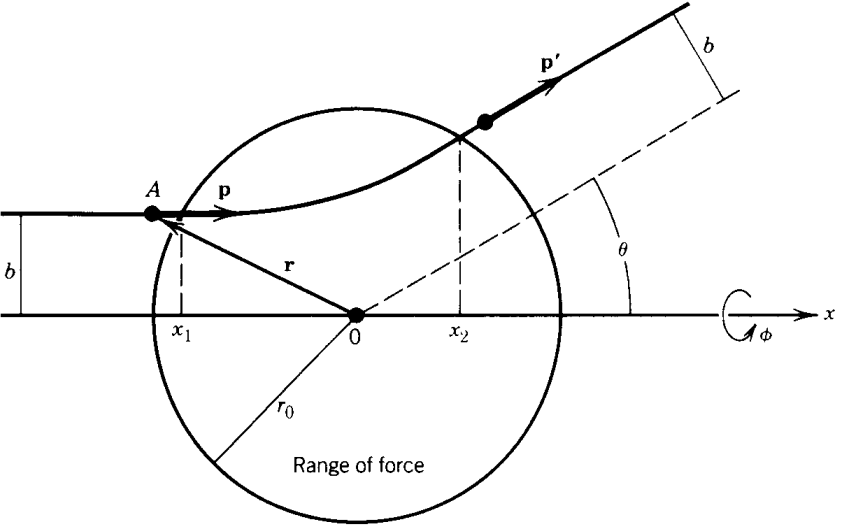
\includegraphics[width=0.6\linewidth]{Immagini/traiettoria particella in campo forze K.png}
    \caption{traiettoria seguita da un particella nel campo di forze $\vk$ centrato in $O$.}
    \label{fig: traiettoria particella in campo forze K}
\end{figure}
Quindi, sempre con riferimento alla figura \ref{fig: traiettoria particella in campo forze K}, si ha un campo di forze agente solo all'interno di un'area finita di raggio $r_0$. Una particella libera con impulso $\vp$ entra in questa area ad una certa distanza $b$, detta ``parametro d'impatto''. All'interno dell'area di interazione, la particella subisce l'azione del campo di forze, viene deflessa ed esce dall'area con un momento $\vp'$, in generale diverso dal momento $\vp$ iniziale, allontanandosi con seguendo una nuova traiettoria. La distanza relativa $\vr$ cambia durante l'interazione, mentre a seconda del valore del parametro d'impatto $b$ variano le coordinate $x_1$ e $x_2$ di uscita. In altre parole, le particelle sono correlate solamente all'interno della zona di interazione, ossia della sfera di raggio $r_0$, invece fuori da essa, la funzione di correlazione coincide con il prodotto di due funzioni di distribuzione di singola particella. Se $f_2$ avesse inizialmente un picco\footnote{Qui ci si riferisce al picco della funzione di distribuzione nello spazio delle fasi.} nel punto $A$, tramite l'equazione \eqref{eq: evoluzione temporale f2} si deduce che il picco si muoverebbe lungo la traiettoria classica rappresentata, definita dalle particolari condizioni iniziali. Invece, all'equilibrio si ha $\p_tf_2 = 0$ e pertanto si ha uno stato stazionario di diffusione nel campo di forze $\vk$ di un fascio di particelle con impulso qualsiasi, a tutti i parametri d'impatto $b$. In altre parole, si ha un flusso stazionario di particelle che seguono la traiettoria classica, a seconda del valore di $b$. Dunque, l'ipotesi del caos molecolare può essere ridefinita tramite le seguenti due affermazioni; all'equilibrio:
\begin{enumerate}
    \item fuori dalla regione di interazione non c'è correlazione e vale l'equazione \eqref{eq: ipotesi caos molecolare};
    \item i valori degli impulsi valutati al bordo della regione di interazione sono correlati, ossia dato l'impulso iniziale $\vp$ e il parametro d'impatto $b$, si può prevedere il valore dell'impulso correlato $\vp'$ a seguito della diffusione.
\end{enumerate}

\subsection{Determinazione di \texorpdfstring{$f_1$}{f1}}
L'obiettivo è adesso quello di determinare la funzione di distribuzione $f_1$. Per farlo, si riparte dalle equazioni \eqref{eq: I e II equazioni BBGKY (ipotesi gas diluito)} supponendo che $f_2$ abbia già raggiunto una situazione di equilibrio, così da ottenere
\begin{equation}
\label{eq: I e II equazioni BBGKY (ipotesi gas diluito + f2 equilibrio)}
    \begin{cases}
        \bigg(\dfrac{\p}{\p t} + \dfrac{\vp_1}{m}\dfrac{\p}{\p \vq_1}\bigg)f_1(1) = \bigg(\dfrac{\p f_1}{\p t}\bigg)_c, \\[2.5ex]
        \bigg[\dfrac{\vp_1}{m}\dfrac{\p}{\p \vq^1} + \dfrac{\vp_2}{m}\dfrac{\p}{\p \vq^2} + \dfrac{1}{2}\vk_{12}\bigg(\dfrac{\p}{\p \vp_1} - \dfrac{\p}{\p \vp_2}\bigg)\bigg]f_2(1,2) = 0.
    \end{cases}
\end{equation}
Riscrivendo la seconda equazione di \eqref{eq: I e II equazioni BBGKY (ipotesi gas diluito + f2 equilibrio)} come
\begin{equation}
\label{eq: processo di interazione 1 e 2}
    \dfrac{1}{2}\vk_{12}\bigg(\dfrac{\p}{\p \vp_1} - \dfrac{\p}{\p \vp_2}\bigg)f_2(1,2) = - \bigg(\frac{\vp_1}{m}\dfrac{\p}{\p \vq^1} + \frac{\vp_2}{m}\dfrac{\p}{\p \vq^2}\bigg) f_2
\end{equation}
e sostituendola nella prima, opportunamente arrangiata, sempre di \eqref{eq: I e II equazioni BBGKY (ipotesi gas diluito + f2 equilibrio)}, si ottiene
\begin{equation}
    \begin{split}
        \bigg(\frac{\p f_1}{\p t}\bigg)_c &= -\int_{r_0}d\mu_2\,\vk_{12}\frac{\p}{\p \vp_1}f_2 \\
        &= -\int_{r_0}d\mu_2\,\vk_{12}\bigg(\frac{\p}{\p \vp_1} - \frac{\p}{\p \vp_2}\bigg)f_2 \\
        &= \frac{2}{m}\int_{r_0}d\mu_2\,\bigg(\vp_1\frac{\p}{\p \vq^1} + \vp_2\frac{\p}{\p \vq^2}\bigg)f_2, 
    \end{split}
\end{equation}
che, a sua volta riscritta in termini delle coordinate del centro di massa e relative \eqref{eq: coordinate CM e relative} e usando la relazione \eqref{eq: relazione tra coordinate lagrangiane e relative}, si ha
\begin{equation}
    \bigg(\frac{\p f_1}{\p t}\bigg)_c = \frac{1}{m}\int_{r_0}d\mu_2\bigg(\vP\frac{\p}{\p \vR} + \vp\frac{\p}{\p \vr}\bigg)f_2.
\end{equation}
Come detto, la funzione $f_1$ varia più lentamente di $f_2$ anche sulle scale spaziali, quindi dal punto di vista di $f_1$, si può considerare che le coordinate prima e dopo l'urto risultino molto simili e pertanto porre $\vq^1\simeq\vq^2$. Inoltre, si può non considerare l'effetto di $\p_{\vR}$ perché nel processo d'urto descritto dalla \eqref{eq: processo di interazione 1 e 2} questo non cambia, essendo la coordinata del baricentro. Dunque, si considera
\begin{equation}
     \bigg(\frac{\p f_1}{\p t}\bigg)_c = \frac{1}{m}\int d^3p_2\int_{r<r_0}d^3r\,\vp\frac{\p f_2}{\p \vr}.
\end{equation}
Dal diagramma in figura \ref{fig: traiettoria particella in campo forze K} si vede che durante la traiettoria vale che
\begin{equation}
    \vp\frac{\p f_2}{\p \vr} = -|\vp|\frac{\p f_2}{\p x},
\end{equation}
inoltre, se si considera un elemento infinitesimo di volume, si ha che questo vale $d^3r = b\,db\,dx\,d\phi$ e quindi si può scrivere
\begin{equation}
    \begin{split}
        \bigg(\frac{\p f_1}{\p t}\bigg)_c &= -\frac{1}{m}\int d^3p_2\,|\vp_2 - \vp_1|\int d\phi\,db\,b\int_{x_1}^{x_2}\frac{\p f_2}{\p x} \\
        &= -\frac{1}{m}\int d^3p_2\,|\vp_2 - \vp_1|\int d\phi\,db\,b[f_2(x_2) - f_2(x_1)],
    \end{split}
\end{equation}
dove gli estremi di integrazione $x_1$ ed $x_2$ sono indipendenti, come si deduce dalla \eqref{eq: processo di interazione 1 e 2}, e dove $f_2(x_1)$ ed $f_2(x_2)$ sono rispettivamente la valutazione di $f_2$ prima e dopo la diffusione. Tuttavia, questi valori di $f_2$ sono valutati sul bordo della regione di interazione. Come detto in precedenza, l'ipotesi del caos molecolare vale unicamente all'interno della regione di interazione: inizialmente si aveva un integrale sulla zona di interazione per cui non si poteva applicare il caos molecolare, ma con le ipotesi fatte si è riusciti a trovare i valori di $f_2$ al bordo di tale regione, dove invece vale il caos molecolare vale. Quindi, è ora possibile rimpiazzare $f_2$ con il prodotto di due funzioni di distribuzione $f_1$ per i due punti
\begin{equation}
    f_2(x_1) \to f_1(\vp_1)f_1(\vp_2),\quad f_2(x_2) \to f_1(\vp_1')f_1(\vp_2'),
\end{equation}
dove $\vp_1$ e $\vp_2$ sono determinati dal processo di diffusione quando gli impulsi iniziali sono $\vp_1$ e $\vp_2$ con un parametro d'impatto $b$. In questa discussione, si è trascurata la dipendenza dalle coordinate $\vq^1$ e $\vq^2$, in quanto si è era considerata l'approssimazione $\vq^1 \simeq \vq^2$. Dunque, si arriva all'espressione
\begin{equation}
\label{eq: espressione f1 in dphi e db}
    \bigg(\frac{\p f_1}{\p t}\bigg)_c = -\frac{1}{m}\int d^3p_2\,|\vp_2 - \vp_1|\int d\phi\,db\,b[f_1(\vp_1')f_1(\vp_2') - f_1(\vp_1)f_1(\vp_2)].
\end{equation}
Il modo in cui compaiono le coordinate è legato alla sezione d'urto differenziale per lo scattering. Si ricorda infatti che, dato un certo flusso di particelle incidenti $I$, per sapere quante particelle vengono diffuse con un certo angolo, si deve calcolare la quantità 
\begin{equation}
    A = I\frac{dG}{d\Omega}d\Omega,
\end{equation}
dove $dG/d\Omega$ è appunto la sezione d'urto differenziale e $A$ è il numero di particelle incidenti diffuse per unità di tempo nell'angolo solido $d\Omega$ intorno alla direzione di $\Omega$.
\begin{figure}[h]
    \centering
    \begin{minipage}[t]{0.55\linewidth}
        \centering
        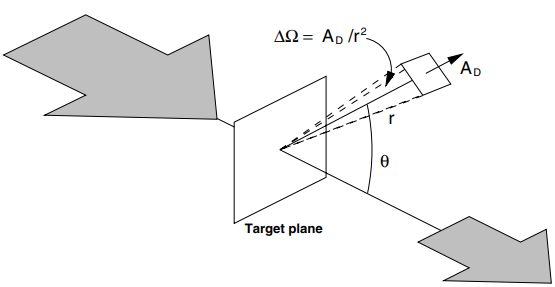
\includegraphics[width=\linewidth]{Immagini/schema scattering.png}
        \caption{schematizzazione della diffusione.}
        \label{fig:schema scattering}
    \end{minipage}
    \hspace{0.8cm}
    \begin{minipage}[t]{0.35\linewidth}
        \centering
        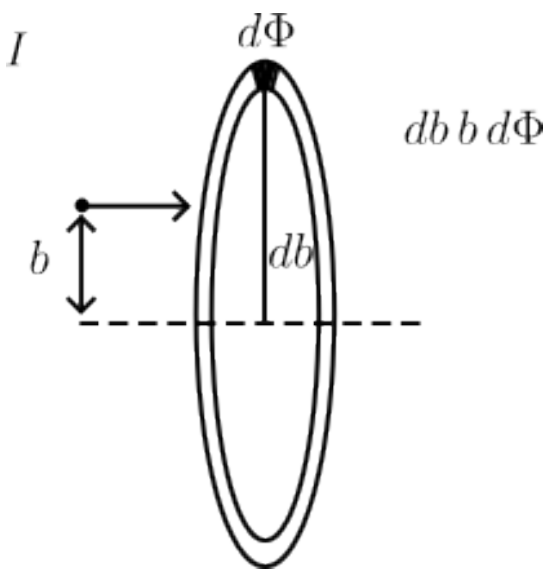
\includegraphics[width=\linewidth]{Immagini/schema per sezione urto.png}
        \caption{analisi per determinare $db\,d\phi$.}
        \label{fig:schema sezione urto}
    \end{minipage}
\end{figure}
Dato che l'angolo di diffusione $\Omega$ è determinato dal parametro d'impatto $b$, sapere qual è il numero di particelle uscenti con un certo angolo $\Omega$ significa conoscere quante sono quelle che entrano con un certo parametro $b$. In altre parole, il numero di particelle diffuse coincide con le particelle entranti in un elemento infinitesimo di superficie perpendicolare al flusso incidente, come mostrato in figura \ref{fig:schema sezione urto}. Quindi, si ha che
\begin{equation}
\label{eq: prodotto db*dphi}
    \cancel{I}\frac{db}{d\Omega}d\Omega = \cancel{I}b\,db\,d\phi\quad\Rightarrow\quad db\,d\phi = \frac{1}{b}\frac{db}{d\Omega}d\Omega.
\end{equation}
Dunque, sostituendo \eqref{eq: prodotto db*dphi} in \eqref{eq: espressione f1 in dphi e db}, si ottiene finalmente l'equazione del trasporto di Boltzmann
\begin{equation}
\label{eq: equazione del trasporto di Boltzmann}
    \bigg(\frac{\p f_1}{\p t}\bigg)_c = -\int d^3p_2\,d\Omega\,|\vv_2 - \vv_1|\frac{db}{d\Omega}\,[f_1(\vp_1')f_1(\vp_2') - f_1(\vp_1)f_1(\vp_2)].
\end{equation}
\begin{notz}
    Per semplicità, dato che nel seguito ci si concentra solo sulla funzione di distribuzione $f_1$, si rinomina $f_1\equiv f$.
\end{notz}
L'equazione del trasporto di Boltzmann fornisce la probabilità che ci siano delle variazioni della funzione di distribuzione di una particella, dovuta alle collisioni con un'altra particella. L'equazione \eqref{eq: equazione del trasporto di Boltzmann} si può reinterpretare come segue
\begin{equation}
\label{eq: equazione del trasporto di Boltzmann in funzione di W}
    \bigg(\frac{\p f}{\p t}\bigg)_c = -\int d^3p_2\,W[(1,2)\to(1',2')][f(2')f(1') - f(2)f(1)],
\end{equation}
dove la funzione $W$ indica la probabilità che avvenga un processo tale per cui lo stato di coppia di particelle $(1,2)$ diventa $(1',2')$, dovuto alla collisione della particella 1 con la particella 2, con $f(1)f(2)$ la probabilità con cui scompare la coppia $(1,2)$, mentre con $f(2')f(1')$ quella con cui compare la coppia $(1',2')$. Dell'equazione \eqref{eq: equazione del trasporto di Boltzmann in funzione di W} si può scrivere l'analogo quantistico
\begin{equation}
\label{eq: equazione del trasporto di Boltzmann quatistica}
    \bigg(\frac{\p f}{\p t}\bigg)_c = -\int d^3p_2\,d^3p_1'\,d^3p_2'\,\delta^4(p_f - p_i)|T_{fi}|^2[f(2')f(1') - f(2)f(1)],
\end{equation}
dove $d^3p_1'\,d^3p_2'$ corrisponde allo spazio delle fasi finale e $|T_{fi}|^2$ è l'elemento di matrice per il processo dallo stato iniziale a quello finale, considerando le possibili interazioni. 

\subsubsection{Distribuzione $f$ all'equilibrio}
Si consideri nuovamente la prima equazione di \eqref{eq: I e II equazioni BBGKY (ipotesi gas diluito)}, dove ora il membro di destra è espresso tramite la \eqref{eq: equazione del trasporto di Boltzmann quatistica}. Si assume che $f \equiv \tilde{f}$ sia in una situazione di equilibrio e che sia omogenea, così da essere indipendente da $\vq^1$, e che sia stazionaria, quindi indipendente da $t$, ovvero $\p_t\tilde{f} = 0$. All'equilibrio continuano ad avvenire fenomeni di scattering tra le particelle, ma questi devono soddisfare la condizione di ``bilancio dettagliato''. Quindi per avere
\begin{equation}
    \bigg(\frac{\p \tilde{f}}{\p t}\bigg)_c = -\int d^3p_2\,d^3p_1'\,d^3p_2'\,\delta^4(p_f - p_i)|T_{fi}|^2[\tilde{f}(2')\tilde{f}(1') - \tilde{f}(2)\tilde{f}(1)] = 0,
\end{equation}
la condizione sufficiente di bilancio dettagliato è ovviamente
\begin{equation}
\label{eq: bilancio dettagliato per f tilde}
    \tilde{f}(2')\tilde{f}(1') = \tilde{f}(2)\tilde{f}(1)\quad\Longrightarrow\quad \p_t\tilde{f} = 0.
\end{equation}
Tuttavia, si può dimostrare che la condizione \eqref{eq: bilancio dettagliato per f tilde} è anche necessaria tramite il teorema H di Boltzmann.

\section{Teorema H}
La quantità $\mathbb{H}$ introdotta da Boltzmann era definita come un funzionale della funzione di distribuzione $f$ in termini della velocità $v$ della particella
\begin{equation}
\label{eq: definizione H}
    \HS = \int d^3v\,f(\vp,t)\log{f(\vp,t)}.
\end{equation}
Se si considerano le proprietà dell'equazione \eqref{eq: definizione H}, è possibile dimostrare, come fece Boltzmann, che essendo $\HS$ limitata inferiormente dal suo valore all'equilibrio, questa non può continuare a decrescere in modo indefinito, ma tende invece al suo valore di equilibrio, mentre contemporaneamente $f$ tende alla distribuzione di Maxwell-Boltzmann. Il teorema H riguarda proprio la dimostrazione dell'andamento non crescente di $\HS$. L'evoluzione temporale di $\HS$ è data da
\begin{equation}
    \frac{d\HS}{dt} = \int d^3v\,\frac{\p f}{\p t}(1 + \log{f}),
\end{equation}
per cui 
\begin{equation}
\label{eq: condizione stazionarietà di f -> stazionarietà di H}
    \frac{\p f}{\p t} = 0 \quad\Rightarrow\quad \frac{d\HS}{dt} = 0
\end{equation}
e la condizione $\dot{\HS} = 0$ è una condizione necessaria affinché $f$ sia stazionaria. Si può dimostrare che la condizione $\dot{H} = 0$ è equivalente a richiedere la relazione di bilancio dettagliato \eqref{eq: bilancio dettagliato per f tilde} quando $f$ soddisfa l'equazione del trasporto di Boltzmann \eqref{eq: equazione del trasporto di Boltzmann}, ossia quando vale l'ipotesi del caos molecolare. Infatti, si considera che 
\begin{equation}
    \begin{split}
        \frac{d\HS}{dt} &= \int d^3v_1\,\frac{\p f(1)}{\p t}(1 + \log{f}) \\
        &= \int\frac{d^3p_1}{m}\bigg(\frac{\p f}{\p t}\bigg)_c[1 + \log{f(1)}] \\
        &= \int\frac{d^3p_1}{m}\int d^3p_2\,d^3p_1'\,d^3p_2'\delta^4(p_f - p_i)|T_{fi}|^2 \\
        &\times[f(1')f(2') - f(1)f(2)][1 + \log{f(1)}].
    \end{split}
\end{equation}
Siccome $|T_{fi}|^2$ è invariante per lo scambio $1 \leftrightarrow 2$ della particella $1$ con la $2$, allora è permesso anche scambiare lo stato iniziale con lo stato finale
\begin{equation}
\label{eq: evoluzione temporale H I}
    \begin{split}
        \frac{d\HS}{dt} &= \frac{1}{2m}\int d^3p_1\,d^3p_2\,d^3p_1'\,d^3p_2'\delta^4(p_f - p_i)|T_{fi}|^2 \\
        &\times[f(1')f(2') - f(1)f(2)][1 + \log{f(1)} + 1 + \log{f(2)}] \\ 
        &= \frac{1}{2m}\int d^3p_1\,d^3p_2\,d^3p_1'\,d^3p_2'\delta^4(p_f - p_i)|T_{fi}|^2 \\
        &\times[f(1')f(2') - f(1)f(2)][2 + \log{f(1)f(2)}].
    \end{split}
\end{equation}
Data l'invarianza di $|T_{fi}|^2$ è anche possibile lo scambio $(1,2) \leftrightarrow (1',2')$ dello stato finale con quello iniziale, ottenendo
\begin{equation}
\label{eq: evoluzione temporale H II}
        \begin{split}
            \frac{d\HS}{dt} &= \frac{1}{2m}\int d^3p_1\,d^3p_2\,d^3p_1'\,d^3p_2'\delta^4(p_f - p_i)|T_{fi}|^2 \\
            &\times[f(1)f(2) - f(1')f(2')][2 + \log{f(1')f(2')}].
        \end{split}
\end{equation}
Le due relazioni trovate \eqref{eq: evoluzione temporale H I} e \eqref{eq: evoluzione temporale H II} sono uguali, pertanto per definire $\dot{H}$ si può considerane una media ottenendo
\begin{equation}
\label{eq: evoluzione temporale H}
    \begin{split}
        \frac{d\HS}{dt} &= \frac{1}{4m}\int d^3p_1\,d^3p_2\,d^3p_1'\,d^3p_2'\delta^4(p_f - p_i)|T_{fi}|^2 \\
        &\times[f(1')f(2') - f(1)f(2)][-\log{f(1')f(2')} + \log{f(1)f(2)}].
    \end{split}
\end{equation}
Per mostrare che l'integrando di \eqref{eq: evoluzione temporale H} non è mai positivo si può considerare la generica funzione di due variabili
\begin{equation}
    h(x,y) = (y - x)(\ln{x} - \ln{y}),\quad x,y > 0,
\end{equation}
dove in questo caso\footnote{In generale, la condizione $x,y > 0$ è relativa al fatto che $x$ ed $y$ sono probabilità.} $y \equiv f(1')f(2')$ e $x \equiv f(1)f(2)$. Quindi, si riscrive $h(x,y)$ come
\begin{equation}
    h(x,y) = y\ln{\bigg(\frac{x}{y}\bigg)}\bigg(1 - \frac{x}{y}\bigg),
\end{equation}
per cui si hanno due casi:
\begin{enumerate}
    \item se il rapporto $x/y \ge 1$, allora $(1 - x/y) \ge 0$ e di conseguenza $h(x,y) \le 0$;
    \item se il rapporto $x/y \le 1$, allora $(1 - x/y) \ge 0$ e di conseguenza $h(x,y) \le 0$.
\end{enumerate}
Dunque, l'equazione \eqref{eq: evoluzione temporale H} coincide con la seguente condizione sul segno di $\HS$ data da $\dot{\HS} \le 0$, particolare il caso di uguaglianza si ha per
\begin{equation}
    \dot{\HS} = 0\quad\Longleftrightarrow\quad \tilde{f}(2')\tilde{f}(1') = \tilde{f}(2)\tilde{f}(1).
\end{equation}
Inoltre, la condizione \eqref{eq: condizione stazionarietà di f -> stazionarietà di H} diventa 
\begin{equation}
    f(1')f(2') - f(1)f(2) = 0 \quad\Longleftarrow\quad \frac{\p f}{\p t} = 0,
\end{equation}
ma si era anche visto dalla \eqref{eq: bilancio dettagliato per f tilde} che 
\begin{equation}
    f(1')f(2') - f(1)f(2) = 0 \quad\Longrightarrow\quad \frac{\p f}{\p t} = 0,
\end{equation}
pertanto le due condizioni sono equivalenti 
\begin{equation}
    f(1')f(2') - f(1)f(2) = 0 \quad\Longleftrightarrow\quad \frac{\p f}{\p t} = 0;
\end{equation}
in particolare, le ipotesi per cui sono equivalenti sono: quella del gas diluito, quella del caos molecolare, quella sull'omogeneità di $f_1$ e il fatto che le variabili $(1,2)$ e $(1',2')$ siano collegate dalla scattering. 

\section{Distribuzione di Maxwell-Boltzmann}
La distribuzione di equilibrio $\tilde{f}(\vp)$ stazionaria deve soddisfare la condizione di bilancio dettagliato \eqref{eq: bilancio dettagliato per f tilde}. 
\begin{notz}
    Per semplicità, nel seguito si indica $\tilde{f} \equiv f$.
\end{notz}
Tale condizione implica che 
\begin{equation}
\label{eq: condizione bilancio dettagliato per f (logaritmica)}
    \log{f(\vp_1')} + \log{f(\vp_2')} = \log{f(\vp_1)} + \log{f(\vp_2)}.
\end{equation}
Si assume ora che lo scattering sia elastico in modo che l'impulso e l'energia cinetica vengano conservati, ossia che
\begin{equation}
    \begin{cases}
        \vp_1 + \vp_2 = \vp_1' + \vp_2' \\
        |\vp_1|^2 + |\vp_2|^2 = |\vp_1'|^2 + |\vp_2'|^2
    \end{cases}.
\end{equation}
La \eqref{eq: condizione bilancio dettagliato per f (logaritmica)} è automaticamente soddisfatta se 
\begin{equation}
    \log{f(\vp)} = a + \vb \cdot \vp - c|\vp|^2,
\end{equation}
dove per ora $a$, $\vb$ e $c$ sono costanti arbitrarie. Se si richiede che la distribuzione di equilibrio corrisponda ad un impulso medio nullo, ovvero che sia invariante per rotazioni, allora deve essere $\vb = 0$, in questo modo la forma generale della funzione di distribuzione risulta essere
\begin{equation}
\label{eq: forma generica distribuzione MB}
    f(\vp) = Ae^{-c|\vp|^2}.
\end{equation}
Si devono adesso imporre alcune condizioni. Prima di tutto, si impone la normalizzazione della funzione $f(\vp)$ come
\begin{equation}
\label{eq: normalizzazione f tilde}
    \int d^3q\,d^3p\,f(\vp) = N,
\end{equation}
inoltre dato che $f(\vp)$ dipende solamente da $|\vp|^2$, allora si può passare in coordinate polari così da avere
\begin{equation}
    \int d^3p\,f(\vp) = 4\pi\int_0^\infty dp\,p^2f(\vp) = \frac{N}{V}.
\end{equation}
Si assume poi nuovamente l'ipotesi del gas diluito, per cui è valida l'equazione di stato termica per i gas monoatomici $E = 3NkT/2$, che adesso si interpreta nel senso che il valor medio dell'energia cinetica per particella debba valere
\begin{equation}
    \bigvmedio{\frac{|\vp|^2}{2m}} = \frac{3}{2}kT,
\end{equation}
da cui segue che
\begin{equation}
\label{eq: ipotesi gas diluito f tilde}
    \int d^3p\,\frac{|\vp|^2}{2m}f(\vp) = \frac{3}{2}\frac{NkT}{V}.
\end{equation}
Passando adesso come prima in coordinate polari, le due condizioni \eqref{eq: normalizzazione f tilde} e \eqref{eq: ipotesi gas diluito f tilde} diventano
\begin{equation}
    \begin{cases}
        4\pi\displaystyle\int_0^\infty dp\,|\vp|^2Ae^{-c|\vp|^2} = \dfrac{N}{V} \\[2ex]
        4\pi\displaystyle\int_0^\infty dp\,\dfrac{|\vp|^4}{2m}Ae^{-c|\vp|^2} = \dfrac{3NkT}{2V}
    \end{cases},
\end{equation}
che, introducendo l'integrale
\begin{equation}
    \int_0^\infty dp\,p^{2k}e^{-cp^2} = \frac{\Gamma(k + 1/2)}{2c^{k + 1/2}} = 
    \begin{cases}
        \dfrac{\Gamma(3/2)}{2c^{3/2}} = \dfrac{\sqrt{\pi}}{4c^{3/2}},\quad k = 1 \\[2ex]
        \dfrac{\Gamma(5/2)}{2c^{5/2}} = \dfrac{3\sqrt{\pi}}{8c^{5/2}},\quad k = 2
    \end{cases},
\end{equation}
diventano
\begin{equation}
\label{eq: normalizzazione f tilde + ipotesi gas diluito f tilde (coord. polari)}
    \begin{cases}
        A\bigg(\dfrac{\pi}{c}\bigg)^{3/2} = \dfrac{N}{V} \\[2ex]
        \dfrac{A}{2mc}\bigg(\dfrac{\pi}{c}\bigg)^{3/2} = \dfrac{NkT}{V}.
    \end{cases}
\end{equation}
Facendo il rapporto delle relazioni \eqref{eq: normalizzazione f tilde + ipotesi gas diluito f tilde (coord. polari)} si trova il valore della costante $c$ come
\begin{equation}
\label{eq: costante c distribuzione MB}
    c = \frac{1}{2mkT},
\end{equation}
il quale sostituito in una delle due condizioni del medesimo sistema restituisce il valore di $A$ come
\begin{equation}
\label{eq: costante A distribuzione MB}
    A = \frac{N}{V(2\pi mkT)^{3/2}}.
\end{equation}
Sostituendo i valori delle due costanti ricavati in \eqref{eq: costante c distribuzione MB} e \eqref{eq: costante A distribuzione MB} nella forma funzionale generica \eqref{eq: forma generica distribuzione MB} si ottiene finalmente la distribuzione di Maxwell-Boltzmann
\begin{equation}
\label{eq: distribuzione MB}
    f(\vp) = \frac{N}{V(2\pi mkT)^{3/2}}\exp{\bigg(-\frac{|\vp|^2}{2mkT}\bigg)}.
\end{equation}

\subsubsection{Osservazioni sul teorema H}
Oltre a determinare la condizione di equilibrio \eqref{eq: bilancio dettagliato per f tilde} individuando così la distribuzione di Maxwell-Boltzmann \eqref{eq: distribuzione MB}, il teorema H di Boltzmann permette anche di affermare che esiste un funzionale $\HS$ della funzione di distribuzione $f$ che per stati diversi da quelli di equilibrio decresce sempre nel tempo. A prima vista, si potrebbe pensare che il funzionale $\HS$ sia in qualche modo proporzionale all'entropia termodinamica $S$ del sistema cambiata di segno. In questo modo, il teorema H sembrerebbe fornire una derivazione dell'irreversibilità macroscopica a partire dalla dinamica microscopica di Liouville. Tuttavia, non è esattamente così, infatti anche se $\HS$ ha un'espressione simile al funzione di entropia di Gibbs, a differenza di $\HS$, l'entropia $S$ non è scritta in termini della funzione di distribuzione della particella singola. Se si prendesse il teorema H come pura conseguenza della dinamica microscopica si andrebbe in contro a dei paradossi, tra cui:
\begin{enumerate}
    \item il ``paradosso dell'irreversibilità'' che riguarda il fatto che il teorema H seleziona una direzione temporale preferenziale che coincide con quella dell'evoluzione irreversibile del sistema, la quale però è incompatibile con la simmetria per inversione temporale della dinamica microscopica;
    \item il ``paradosso della ricorrenza'', legato ai cicli di Poincaré, consiste nel fatto che un sistema preparato in uno stato generico, anche se dovesse raggiungere l'equilibrio, non ci rimarrebbe indefinitamente dato che, su un tempo sufficientemente lungo, il sistema ripassa arbitrariamente vicino allo stato iniziale infinite volte. 
\end{enumerate}
Tuttavia, questi paradossi sono risolti da diverse considerazioni. Inoltre, il teorema H non deriva unicamente dalla dinamica microscopica tramite il teorema di Liouville e le sue conseguenze, ma sfrutta anche l'ipotesi del caos molecolare. In realtà il teorema H afferma che:
\begin{quote}
    ``se ad un istante $t$ vale l'ipotesi del caos molecolare\footnote{L'ipotesi del caos molecolare riguarda $f_2$ non $f_1$, quindi può essere verificata o meno per qualunque $f$.}, allora ad un istante successivo $t' = t + \epsilon$ si ha $\dot{\HS}(t') \le 0$ e la funzione di distribuzione $f(\vp)$ coincide con la distribuzione di Maxwell-Boltzmann.''
\end{quote}
Sfruttando l'invarianza per inversione temporale, si può dedurre che se l'ipotesi del caos molecolare è valida ad un istante $t$, allora si ha
\begin{equation}
    \begin{cases}
        \dfrac{d\HS}{dt} \le 0,\quad t' = t + \epsilon \\[2ex]
        \dfrac{d\HS}{dt} \ge 0,\quad t' = t - \epsilon 
    \end{cases};
\end{equation}
dunque, nell'istante $t$ il funzionale $\HS$ è discontinuo e presenta un picco locale quando vale l'ipotesi del caos molecolare con $f$ che non coincide con la distribuzione di Maxwell-Boltzmann \eqref{eq: distribuzione MB} all'equilibrio, come mostrato in figura \ref{fig: picco locale (teo. H)}.
\begin{figure}[h]
    \centering
    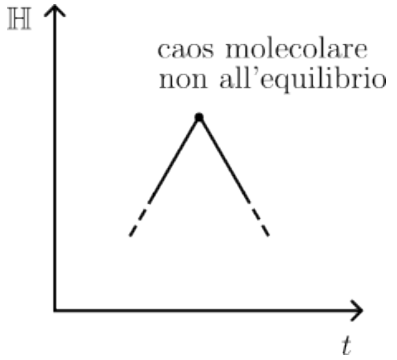
\includegraphics[width=0.35\linewidth]{Immagini/picco locale (teo. H).png}
    \caption{picco locale di $\HS$ fuori dall'equilibrio.}
    \label{fig: picco locale (teo. H)}
\end{figure}

In generale, per un sistema in uno stato diverso da uno di equilibrio non vale l'ipotesi del caos molecolare: gli urti fra le componenti posso crearlo o distruggerlo. L'andamento di $\HS$ riscontrato nelle simulazioni con $N$ abbastanza grande, il quale è in accordo con l'approccio all'equilibrio dei sistemi reali, può essere compreso sulla base delle seguenti, plausibili ma non dimostrate, asserzioni:
\begin{enumerate}
    \item il funzionale $\HS$ è minimo quando la funzione di distribuzione è quella di Maxwell-Boltzmann;
    \item gli urti molecolari hanno un carattere casuale, la sequenza temporale degli stati del gas è scelta casualmente tra i microstati possibili per fissate condizioni macroscopiche;
    \item gli stati di equilibrio sono i più numerosi.
\end{enumerate}
Inoltre, in rifermento al primo grafico in figura \ref{fig: andamento di H}, il comportamento osservato di $\HS$ è il seguente:
\begin{itemize}
    \item se lo stato macroscopico iniziale è prossimo all'equilibrio, vi sono di norma solo piccole fluttuazioni di $\HS$, mentre più $\HS$ si allontana dal valore di equilibrio, più il sistema stesso si è allontana da esso. Tuttavia, questo avviene raramente e il sistema entra ed esce rapidamente da tale stato, con la conseguenza che $\HS$ presenta un picco locale molto pronunciato;
    \item se il sistema viene preparato in uno stato molto fuori equilibrio, siccome tale stato, se occorresse spontaneamente darebbe luogo ad un picco molto pronunciato, è molto probabile un'immediata discesa di $\HS$ che poi ``in media'', ripetendo il ragionamento, continua a scendere verso l'equilibrio.
\end{itemize}
In sostanza, quando il sistema è lontano dall'equilibrio sono più numerose le configurazioni che portano a una diminuzione di $\HS$ rispetto a quelle che la aumentano. Quindi in media $\HS$ decresce, anche se ci sono dei momenti in cui non vale l'ipotesi del caos molecolare. Quindi, il teorema H è una sorta di meccanismo di controllo che impedisce di allontanarsi dall'equilibrio. Questi comportamenti sono stati dimostrati rigorosamente per il modello in cui le particelle sono ``hardspheres'', nel limite dei gas diluiti (teorema di Landford). Si dimostra in tal caso che l'evoluzione di $f$ è guidata dall'equazione di Boltzmann per la stragrande maggioranza degli stati.
\begin{figure}[h]
    \centering
    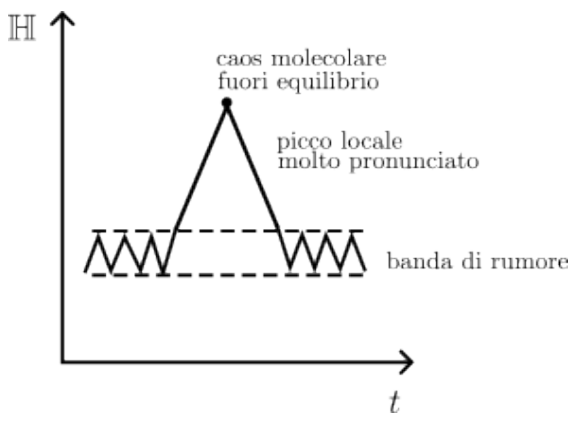
\includegraphics[width=0.45\linewidth]{Immagini/andamento di H (teo. H) 1.png}
    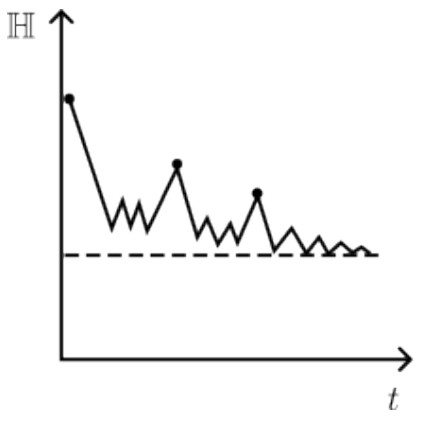
\includegraphics[width=0.35\linewidth]{Immagini/andamento di H (teo. H) 2.png}
    \caption{andamento di $\HS$ per uno stato iniziale: (i) prossimo all'equilibrio; (ii) molto fuori equilibrio.}
    \label{fig: andamento di H}
\end{figure}

\chapter{Meccanica statistica quantistica}
Anche se la descrizione classica spesso fornisce un'utile approssimazione, la trattazione corretta dei sistemi a livello microscopico è quella quantistica. Serve quindi anche in questo contesto capire come possa emergere il comportamento termodinamico a livello macroscopico. Dato un sistema quantistico, anche a più componenti, esso è descritto da uno stato $\ket{\psi}$ in uno spazio di Hilbert. Lo stato $\ket{\psi}$ può venire espresso in una qualsiasi combinazione in una qualsivoglia base conveniente allo scopo. Ad esempio, se $\ket{q}$ è un autostato dell'operatore posizione, allora $\ket{\psi}$ si può scrivere come
\begin{equation}
    \ket{\psi} = \int dq\,\ket{q}\mybraket{q}{\psi},\quad \mybraket{q}{\psi(t)} = \psi(q,t).
\end{equation}
L'evoluzione temporale di $\ket{\psi}$ è determinata dall'equazione di Schr\"odinger 
\begin{equation}
\label{eq: equazione di Schrodinger}
    i\hbar\frac{\p}{\p t}\ket{\psi(t)} = \hatH\ket{\psi(t)}.
\end{equation}
Questo implica che la dinamica è reversibile rispetto al tempo e l'evoluzione è unitaria. Si arriva di fronte allo stesso problema già incontrato nel contesto classico: come può emergere l'evoluzione macroscopica irreversibile verso l'equilibrio in cui raggiunge la stazionarietà? Perché c'è un macrostato unico di equilibrio che ``dimentica\footnote{In Termodinamica si parla di funzioni di stato che hanno la caratteristica di dipendere solo dallo stato che il sistema termodinamico ha in quel preciso momento, dimenticandosi dei trascorsi precedenti.}'' le condizioni iniziali? Come nel caso classico, il problema è ancora oggi oggetto di dibattito. Ci si concentra quindi sulla teoria standard degli ensembles statistici in versione quantistica. 

\subsubsection{Evoluzione di uno stato puro}
Sia $\{n\}$ il set di autovalori di un sistema completo di osservabili commutanti, tra le quali l'hamiltoniana, e si indichi con $\{\ket{n}\}$ il set dei corrispondenti autostati, quindi si ha dall'equazione agli autovalori dell'hamiltoniana
\begin{equation}
    \hatH\ket{n} = E_n\ket{n}
\end{equation}
che l'evoluzione degli stati $\ket{n}$ è completamente determinata da
\begin{equation}
    \ket{n(t)} = e^{-iE_nt/\hbar}\ket{n}.
\end{equation}
Un generico stato puro si può espandere, tramite una somma o un integrale a seconda che i livelli siano discreti o continui rispettivamente, come
\begin{equation}
    \ket{\psi(t)} = \sumint c_n\ket{n(t)} = \sumint c_ne^{-iE_nt/\hbar}\ket{n}.
\end{equation}
Quindi, noto lo spettro, risulta completamente determinato lo stato iniziale a $t = 0$ come
\begin{equation}
    \ket{\psi(0)} = \sumint c_n\ket{n}.
\end{equation}
Ora, il valore medio, definito nei termini quantistici, di un'osservabile $\hatO$, cioè di un operatore autoaggiunto definito su uno spazio di Hilbert, nello stato $\ket{\psi(t)}$ è dato da
\begin{equation}
    \begin{split}
        \vmedio{\hatO}_{\ket{\psi(t)}} &= \mybrakett{\psi(t)}{\hatO}{\psi(t)} \\
        &= \nsum_{m,n} c_m^*c_ne^{i(E_m - E_n)t/\hbar}\mybrakett{m}{\hatO}{n} \\
        &= \nsum_n|c_n|^2\mybrakett{n}{\hatO}{n} + \nsum_{m\neq n}c_m^*c_ne^{i(E_m - E_n)t/\hbar}\mybrakett{m}{\hatO}{n},
    \end{split} 
\end{equation}
da cui si deduce che, per un generico stato $\ket{\psi(t)}$ ed una generica osservabile $\hatO$, non si ha un'evoluzione verso l'equilibrio in quanto:
\begin{enumerate}
    \item il primo termine a secondo membro è indipendente dal tempo, anche nel limite $t\to\infty$, per cui è stazionario, anche se tuttavia dipende dallo stato iniziale attraverso i coefficienti $c_n$ e quindi non perde ``memoria'' di esso;
    \item il secondo termine del secondo membro nel limite $t\to\infty$ continua ad oscillare nel tempo non diventando perciò mai stazionaria.
\end{enumerate}
Dunque, l'evoluzione di uno stato puro non è adatta a descrivere l'evoluzione termodinamica verso l'equilibrio. In altre parole, con uno stato puro non ci si aspetta termalizzazione per un sistema quantico isolato. 

\subsubsection{Meccanismi di termalizzazione}
Prima di tutto si da una definizione adatta di ``termalizzazione'' di un sistema secondo la Meccanica statistica.
\begin{defn}[termalizzazione]
    La termalizzazione è il processo secondo il quale le particelle di un sistema fisico giungono all'equilibrio termico mediante successive mutue interazioni.
\end{defn}
Si assume, nell'approccio standard della Meccanica statistica, che la termalizzazione nei sistemi quantistici macroscopici sia legata ai seguenti fatti: la conoscenza incompleta dello stato e le interazioni con l'ambiente.

\paragraph{Conoscenza incompleta dello stato.} Anche ammettendo di conoscere lo spettro, cioè di aver risolto l'equazione di Scr\"odinger stazionaria, per specificare lo stato $\ket{\psi}$ si dovrebbero conoscere con estrema precisione tutti i coefficienti $c_n$ dello sviluppo, che però sono un numero enorme. Infatti, i livelli energetici per un sistema con un numero elevato $N$ di componenti sono molto densi e gli stati iniziali del sistema macroscopico sono quindi sempre specificati con un certo grado di incertezza.

\paragraph{Interazioni con l'ambiente.}  Anche il sistema reale meglio isolato è in realtà, quasi-isolato. Infatti, data la densità dei livelli, basta qualsiasi anche minima interazione con l'ambiente per alterare i livelli stessi e lo stato del sistema. Tra le interazioni, nel caso quantistico, vanno incluse anche quelle con gli apparati di misura.

\section{Matrice densità}
Per quanto detto, adesso si considerano sistemi di cui non si ha una conoscenza completa. La descrizione quantistica basata su un insieme di dati incompleto si sviluppa tramite il formalismo della matrice densità, che è lo stesso utilizzato nella teoria degli ensembles statistici. 

Si supponga quindi di conoscere in modo incompleto lo stato di un sistema, conoscendo solo la probabilità $p_k$ che il sistema si trovi in un certo stato $\ket{\psi_k(t)}$ dove l'insieme $\{\ket{\psi(t)}\}$ non è detto che rappresenti un sistema completo. Essendo $p_k$ delle probabilità, devono soddisfare la normalizzazione 
\begin{equation}
\label{eq: normalizzazione pk}
    \nsum_k p_k = 1,\quad 0 \le p_k \le 1.
\end{equation}
In questo caso, data l'incertezza sullo stato assunto dal sistema, la predizione della misura di un'osservabile $\hatO$ non è più il semplice valor medio quantistico, ma è un valore medio in senso statistico pesato dalle $p_k$ sui contributi dei valori medi quantistici dei vari stati, ossia
\begin{equation}
\label{eq: valore medio quatistico statistico}
    \vmedio{\hatO} = \nsum_k p_k\vmedio{\hatO}_k = \nsum_k p_k\mybrakett{\psi_k(t)}{\hatO}{\psi_k(t)}.
\end{equation}
L'espressione \eqref{eq: valore medio quatistico statistico} può essere riscritta in termini dell'operatore densità $\hatrho$ definito come
\begin{equation}
\label{eq: definizione operatore densità}
    \hatrho := \nsum_k p_k \ket{\psi_k(t)}\bra{\psi_k(t)},
\end{equation}
dove $\ket{\psi_k(t)}$ e $\bra{\psi_k(t)}$ sono i proiettori sugli stati $\psi_k(t)$, ottenendo
\begin{equation}
\label{eq: valore medio quantistico statistico (operatore densità)}
    \vmedio{\hatO} = \Tr{\hatO\hatrho}.
\end{equation}
Infatti, se $\{\ket{\alpha}\}$ è una qualsiasi base completa, introducendo una relazione di completezza $\nsum_\alpha\ket{\alpha}\bra{\alpha} = \MI$, si può scrivere
\begin{equation}
    \begin{split}
        \vmedio{\hatO} = \Tr{\hatO\hatrho} &= \nsum_k\nsum_\alpha p_k \mybrakett{\psi_k(t)}{\hatO}{\alpha}\mybraket{\alpha}{\psi_k(t)} \\
        &= \nsum_\alpha\mybrakett{\alpha}{\nsum_k p_k}{\psi_k(t)}\mybrakett{\psi_k(t)}{\hatO}{\alpha} \\
        &= \nsum_\alpha\mybrakett{\alpha}{\hatrho\hatO}{\alpha} \\
        &= \Tr{\hatrho\hatO}.
    \end{split}
\end{equation}
Nella definizione di valore medio \eqref{eq: valore medio quantistico statistico (operatore densità)}, l'operatore $\hatrho$ compare come una traccia. Quindi, la descrizione è indipendente dalla particolare base che si decide di scegliere per rappresentare l'operatore. Questo fatto è molto conveniente in quanto la scelta di una certa base piuttosto che un'altra può semplificare la descrizione di un particolare sistema. Fissata la base, l'operatore $\hatrho$ è descritto dai suoi elementi di matrice, per questo si parla di ``matrice densità'' $\rho_{\alpha\beta}$, tipicamente rappresentata nella base dell'energia. 

L'operatore e la matrice densità posseggono alcune proprietà importanti. Per studiarle, si supponga di scegliere una base $\{\ket{\alpha}\}$, l'operatore $\hatrho$ è quindi rappresentato dalla matrice densità
\begin{equation}
    \rho_{\alpha\beta} = \mybrakett{\alpha}{\hatrho}{\beta}.
\end{equation}
Le proprietà in questione sono:
\begin{enumerate}
    \item $\Tr{\hatrho} = 1$, infatti se si applica la definizione \eqref{eq: valore medio quantistico statistico (operatore densità)} nel caso in cui $\hatO \equiv \MI$, si ha direttamente $\vmedio{\MI} = 1 = \Tr{\hatrho}$;
    \item $\rho_{\alpha\alpha} \le 1$, infatti si ha che
    \begin{equation}
        \rho_{\alpha\alpha} = \nsum_k p_k\mybraket{\alpha}{\psi_k(t)}\mybraket{\psi_k(t)}{\alpha} = \nsum_k p_k |\mybraket{\alpha}{\psi_k(t)}|^2,
    \end{equation}
    ma considerando la condizione \eqref{eq: normalizzazione pk} e dato che $|\mybraket{\alpha}{\psi_k(t)}|^2 \le 1$, allora è immediato vedere che $\rho_{\alpha\alpha} \le 1$;
    \item dato che la precedente proprietà è valida per qualunque base, si indica con $\{\ket{\Lambda_i}\}$ la base di $\hatrho$ tale che $\hatrho\ket{\Lambda_i} = \lambda_i\ket{\Lambda_i}$, allora 
    \begin{equation}
        \lambda_i = \mybrakett{\Lambda_i}{\hatrho}{\Lambda_i} \le 1,\quad \nsum_i\lambda_i = \Tr{\hatrho} = 1,
    \end{equation}
    da cui, dato che $\lambda_i^2 \le \lambda_i$, si ricava che
    \begin{equation}
        \Tr{\hatrho^2} = \nsum_i\lambda_i^2 \le \nsum_i\lambda_i \le 1,
    \end{equation}
    dunque, si ha
    \begin{equation}
        \Tr{\hatrho^2} \le 1;
    \end{equation}
    \item $\Tr{\hatrho^2} = 1$ se e solo se il sistema si trova in uno stato puro, infatti, se si suppone che $\hatrho$ si possa scrivere come $\hatrho = \ket{\psi}\bra{\psi}$ per un qualche stato puro, allora solo in tal caso, siccome $\ket{\psi}\bra{\psi}$ è un proiettore, si ha
    \begin{equation}
        \hatrho = \ket{\psi}\bra{\psi} \quad\Rightarrow\quad \Tr{\hatrho^2} = 1;
    \end{equation}
    \item i termini non diagonali di $\rho_{\alpha\beta}$, con $\alpha \neq \beta$, non hanno direttamente significato di probabilità che il sistema sia in un certo stato $\alpha$, ma rappresentano piuttosto la tendenza del sistema di passare dallo stato $\ket{\beta}$ allo stato $\ket{\alpha}$, pertanto all'equilibrio ci si aspetta che 
    \begin{equation}
        \rho_{\alpha\beta} = \rho_{\beta\alpha},
    \end{equation}
    ossia che la matrice densità soddisfi una condizione di bilancio dettagliato.
\end{enumerate}
L'operatore densità svolge un ruolo analogo a quello della densità di probabilità $\rho(q,p)$ nella discussione classica. Allo stesso modo, la sua evoluzione temporale è determinata dalla dinamica microscopica, ma al posto che essere descritta dall'equazione di Liouville, lo è dall'equazione di Schr\"odinger
\begin{equation}
\label{eq: evoluzione temporale operatore densità (eq. schrodinger)}
    i\hbar\frac{\p \hatrho}{\p t} = \comm{\hatH}{\hatrho}.
\end{equation}
Essendo stati puri, si sa che l'evoluzione è unitaria
\begin{equation}
    \hatrho(t) = e^{-i\hatH t/\hbar}\hatrho(0)e^{i\hatH t/\hbar}.
\end{equation}
Il risultato della \eqref{eq: evoluzione temporale operatore densità (eq. schrodinger)} è l'analogo del teorema di Liouville \eqref{eq: equazione di Liouville} per il caso classico, infatti
\begin{equation}
\label{eq: evoluzione temporale operatore densità (eq. liouville)}
    \frac{\p \rho}{\p t} = \acomm{H}{\rho}.
\end{equation}
Come al solito, nel passaggio dalla trattazione classica a quella quantistica le parentesi di Poisson vengono sostituire con il commutatore. 
\begin{obs}
    Al momento si sta lavorando nella rappresentazione di Schr\"odinger dove gli stati evolvono nel tempo, mentre le osservabili sono stazionarie. Tuttavia, $\hatrho$, che è un operatore definito su uno spazio di Hilbert, è dipendente dal tempo.
\end{obs}
Nel caso classico, all'equilibrio ci si aspetta che $\rho(q,p)$ sia stazionaria, per cui anche $\hatrho$ deve risultare stazionaria all'equilibrio e quindi dall'equazione \eqref{eq: evoluzione temporale operatore densità (eq. schrodinger)} segue che
\begin{equation}
    \comm{\hatH}{\hatrho} = 0,
\end{equation}
ossia $\hatrho$ deve essere esprimibile tramite osservabili commutanti con l'hamiltoniana. Si assuma pertanto, per le medesime ragioni del caso classico, che $\hatrho$ dipenda solo da $\hatH$, o al massimo dall'operatore numero $\hatN$, il cui autovalore è il numero di particelle del sistema, se quest'ultimo è aperto. All'equilibrio, $\hatrho$ è convenientemente rappresentato nella base dell'energia degli stati stazionari $\ket{n}$ in cui, commutando con $\hatH$, esso è diagonale
\begin{equation}
    \hatrho = \nsum_n p_n\ket{n}\bra{n}.
\end{equation}
In tale base, $\hatrho$ è rappresentato da una matrice densità diagonale
\begin{equation}
\label{eq: matrice densità diagonale}
    \rho_{mn} = p_n\delta_{mn},
\end{equation}
dove $p_n$ coincide con la probabilità che il sistema si trovi nello stato $\ket{n}$ con energia pari a $E_n$.

\subsubsection{Entropia di von Neumann}
In Meccanica quantistica, nel formalismo della matrice densità, si introduce l'entropia di von Neumann
\begin{equation}
\label{eq: definizione entropia von Neumann}
    \SvN := -\Tr{\hatrho\ln{\hatrho}} = -\nsum_i\lambda_i\ln{\lambda_i}.
\end{equation}
Questa entropia rappresenta una misura dell'informazione quantistica contenuta in uno stato. Infatti, si ha $\SvN = 0$ per uno stato puro, mentre $\SvN > 0$ per uno stato misto\footnote{Infatti, se $\hatrho$ corrisponde ad uno stato puro, allora corrisponde un unico autovalore $\lambda_i = 1$, mentre gli altri sono nulli, per cui $\SvN = 0$; invece, se corrisponde ad uno stato misto, allora il logaritmo è negativo e $\SvN > 0$.}. L'espressione \eqref{eq: definizione entropia von Neumann} è analoga all'espressione dell'entropia di Shannon in Teoria dell'informazione. Inoltre, l'entropia di von Neumann per sistemi con molte componenti coincide, a meno di un fattore globale dato dalla costante di Planck, con l'entropia del sistema. 
\chapter{Ensemble microcanonico}
Il concetto fondamentale alla base dell'approccio statistico consiste, per un'osservabile $O$, nella relazione
\begin{equation}
    O = \nsum_\nu P(\nu)O(\nu) \equiv \vmedio{O},
\end{equation}
dove $\{\nu\}$ è l'insieme dei microstati compatibili con lo stato macroscopico del sistema considerato e $\vmedio{O}$ è una media statistica sull'insieme di tali microstati, in quanto pesata con la probabilità $P(\nu)$. Per poter sfruttare questo approccio è necessario:
\begin{enumerate}
    \item determinare la forma generale di $P(\nu)$ per i diversi tipi di sistemi in funzione delle variabili microscopiche;
    \item esprimere le quantità termodinamiche rilevanti per i diversi sistemi in termini di $P(\nu)$.
\end{enumerate}
L'ensemble microcanonico corrisponde ad un sistema isolato:
\begin{enumerate}
    \item chimicamente, quindi il numero di particelle $N$ è fissato e non avvengono decadimenti e/o aggregazioni;
    \item meccanicamente, per cui il volume $V$ è finito e il sistema non si espande e comprime;
    \item termicamente, ovvero le pareti del contenitore non permettono uno scambio di energia $E$.
\end{enumerate} 
Pertanto, le variabili di controllo consistono in $\{E,V,N\}$, tutte grandezze di carattere estensivo. Quindi, l'ensemble microcanonico è l'ensemble dei microstati che il sistema può assumere quando sono fissate queste variabili. Tuttavia, nella realtà non si può fissare completamente l'energia, infatti si ha un'inevitabile incertezza per cui i microstati $\nu$ dell'ensemble microcanonico con energia $E$ sono tali che
\begin{equation}
    E \le E(\nu) \le E + \Delta,\quad \frac{\Delta}{E} \ll 1.
\end{equation}
Se ci si pone nello spazio delle fasi, si osserva che i microstati si trovano su un livello di energia definita dall'ipersuperficie di energia fissata $E$ e dalla corona $E + \Delta$, come mostrato in figura \ref{fig: spazio delle fasi microcanonico}.
\begin{figure}[h]
    \centering
    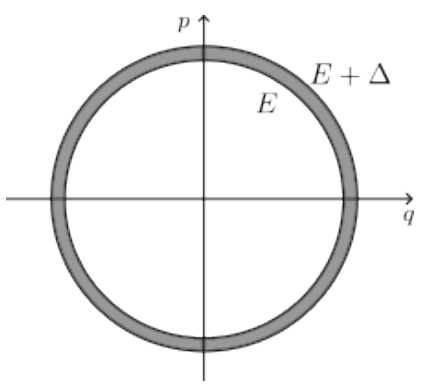
\includegraphics[width=0.35\linewidth]{Immagini/spazio delle fasi microcanonico.png}
    \caption{ensemble microcanonico dei microstati nello spazio delle fasi.}
    \label{fig: spazio delle fasi microcanonico}
\end{figure}

All'equilibrio, si può assumere che la probabilità $P(\nu)$ dipenda solo dall'energia, in quanto, dato che deve essere stazionaria, deve avere parentesi di Poisson nulle con l'operatore di Liouville nel caso classico, dove $P(\nu) \equiv \rho(q,p)$, o con l'hamiltoniana nel caso quantistico, potendo quindi dipendere solo da costanti del moto, in questo caso l'energia $E$. Essendo l'energia $E$ fissata per tutti i microstati, anche $P(\nu)$ deve esserlo, ma allora è anche indipendente da $\nu$ e tutti i microstati sono equiprobabili. Sia ora $\Omega(E,V,N)$ il numero di $\nu$ nell'ensemble, ossia il numero di quelli che si trovano nello stesso livello di energia, allora la condizione di normalizzazione della probabilità $P(\nu) \equiv P$ implica che 
\begin{equation}
\label{eq: probabilità microstati (microcanonico)}
    \sum_{\nu = 1}^\Omega P(\nu) = \Omega P = 1\quad\Rightarrow\quad P = \frac{1}{\Omega(E,V,N)}.
\end{equation}

\subsubsection{Ergodicità}
In generale, un sistema isolato è descrivibile tramite l'ensemble microcanonico se la media temporale delle osservabili è effettivamente uguale alla media di ensemble 
\begin{equation}
\label{eq: media ensemble microcanonico}
    \bar{O} = \sum_{\nu = 1}^\Omega P(\nu)O(\nu) = \frac{1}{\Omega}\sum_{\nu = 1}^\Omega O(\nu),
\end{equation}
cioè se, per tempi sufficientemente lunghi, il sistema visita tutti gli stati accessibili con la stessa frequenza. Un sistema che presenta tale comportamento è detto ``ergodico''. Nel suo moto sul livello di energia fissata, il sistema passa arbitrariamente vicino ad ogni punto, ossia ad ogni microstato, ed il tempo che trascorre in ognuna sottoregione è proporzionale all'area della stessa. 

Tuttavia, l'ergodicità di un sistema dinamico a molti corpi è difficile da stabilire rigorosamente, anche se i sistemi reali, in buona approssimazione, sono quasi sempre ergodici. Si presentano infatti alcuni problemi:
\begin{enumerate}
    \item secondo il teorema KAM anche sotto perturbazioni, certi sistemi dinamici continuano a seguire traiettorie confinate in certe sottoregioni individuate dalle condizioni iniziali, non diventando mai caotici;
    \item nelle simulazioni numeriche il comportamento ergodico fatica ad emergere.
\end{enumerate}
Anche ammettendo che ci fosse un comportamento ergodico, la media statistica \eqref{eq: media ensemble microcanonico} sarebbe giustificata se il tempo di misura $t$ fosse comparabile con il tempo di ritorno $T$ impiegato dal sistema per ritornare nei pressi dello stato iniziale. Tuttavia, se nella dinamica c'è una piccola componente causale, necessaria per la termalizzazione, allora per il lemma di Kac ci si può aspettare che il tempo di ritorno cresca esponenzialmente con il numero di componenti, e quindi i tempi di ritorno siano estremamente lunghi 
\begin{equation}
    T \simeq \tau_c e^{\alpha N},
\end{equation}
dove $\tau_c$ è il tempo di scala della collisioni molecolari e $\alpha$ è lo stesso coefficiente che compare per la probabilità di un microstato, la quale invece decresce in funzione di $N$ come $P(\nu) \simeq e^{-\alpha N}$. Dunque, il tempo di ritorno $T$ è in genere fuori scala per qualsiasi applicazione reale, pertanto l'ergodicità potrebbe nella pratica essere una condizione irrilevante. 

D'altra parte, le osservabili di interesse in Termodinamica sono tipicamente one-body o two-body, quindi ciò che ci interessa realmente è che per tali osservabili valga l'uguaglianza \eqref{eq: media ensemble microcanonico} per quasi tutte le condizioni iniziali e sia approssimativamente valida nel limite $N\to\infty$ anche per tempi $t$ relativamente brevi e non
comparabili con il tempo di ritorno. Esistono risultati rigorosi nel contesto dei gas ideali e/o con interazioni a corto raggio che mostrano che tali osservabili sono in effetti ``self-averaging'': per $N\to\infty$ assumono un valore praticamente costante su quasi tutti i microstati accessibili e pertanto la media temporale viene a coincidere con la media statistica. 

\section{Entropia microcanonica}
Determinata la distribuzione di equilibrio, l'obiettivo adesso è quello di determinare la termodinamica, in particolare trovando un'espressione dell'entropia. Ci si aspetta che $\Omega(E,V,N)$ sia legato alla funzione che determina la termodinamica a fissate $\{E,V,N\}$, ovvero all'entropia $S(E,V,N)$. Si deve pertanto dedurre la relazione tra $\Omega$ e $S$. Per farlo, si considerano due sistemi microcanonici all'equilibrio termico posti a contatto, come mostrato in figura \ref{fig: sistemi per entropia (microcanonico)}. I due sistemi sono inizialmente isolati da una barriera, per cui il numero complessivo di microstati è
\begin{equation}
    \Omega(E) = \Omega_1(E_1,V_1,N_1)\Omega_2(E_2,V_2,N_2) \equiv \Omega_1(E_1)\Omega_2(E_2),
\end{equation}
data l'indipendenza dei due sistemi e l'invarianza dei due volumi e dei numeri di particelle in ciascuno di essi. 
\begin{figure}[h]
    \centering
    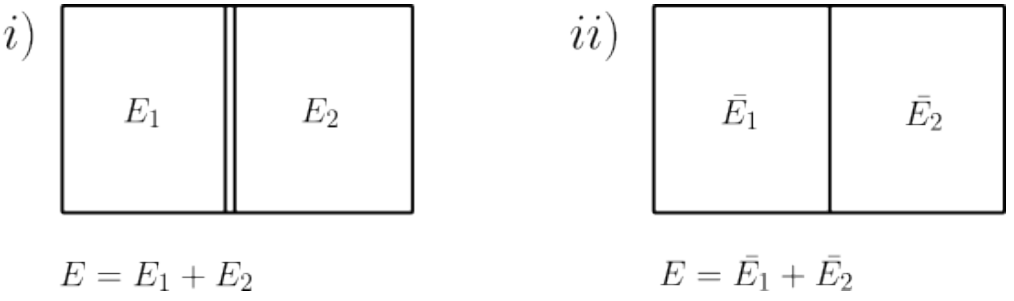
\includegraphics[width=0.65\linewidth]{Immagini/sistemi per entropia (microcanonico).png}
    \caption{sistemi nello stato: (i) iniziale e separati; (ii) finale e uniti.}
    \label{fig: sistemi per entropia (microcanonico)}
\end{figure}
Quando la barriera viene rimossa, i due sistemi sono posti a contatto e avviene uno scambio termico, pur rimanendo il sistema globalmente isolato. In questo momento il sistema non è più in equilibrio e nuovi microstati diventano disponibili con una diversa distribuzione di energia tra i due sottosistemi. Quindi, il numero di microstati possibili ora è dato da
\begin{equation}
\label{eq: microstati complessivi (microcanonico)}
    \Omega(E) = \int dE_1\,\Omega_1(E_1)\Omega_2(E_2),\quad E_2 \equiv E - E_1.
\end{equation}
L'idea consiste nel pensare che $\Omega(E)$ tende a evolvere fino a raggiungere un valore massimo nella nuova situazione di equilibrio, per un certo valore $\bar{E}_1$ e $\bar{E}_2 = E - \bar{E}_1$ delle energie dei due sistemi. Infatti, all'equilibrio, tra tutti i possibili valori di $E_1$ c'è uno che domina, contrassegnato da $\bar{E}_1$. Dunque, si assume che il macrostato di equilibrio sia quello che corrisponde al maggior numero possibile di microstati. 

Per vedere ciò, si considera un sistema composto da un gas inizialmente preparato in una situazione fuori equilibrio. Le componenti sono confinate in una sottoregione delimitata da una barriera, ma alla rimozione di questa il gas tende ad espandersi arrivando all'equilibrio occupando tutto il volume disponibile, come mostrato in figura \ref{fig: evoluzione sistema (microcanonico)}. 
\begin{figure}[h]
    \centering
    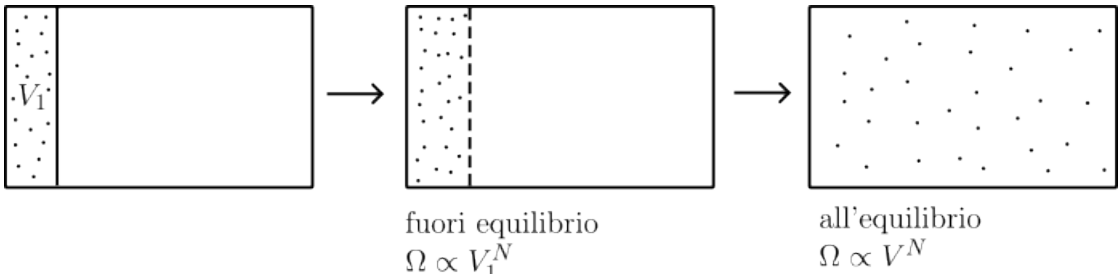
\includegraphics[width=0.75\linewidth]{Immagini/evoluzione sistema (microcanonico).png}
    \caption{evoluzione temporale di un gas verso lo stato di equilibrio.}
    \label{fig: evoluzione sistema (microcanonico)}
\end{figure}
A livello classico, il numero di microstati disponibili è proporzionale al volume dello spazio delle fasi permesso, in particolare cresce con il volume $V$ secondo $V^N$. Appena viene rimossa la barriera $\Omega \propto V_1^N$, ma avvicinandosi all'equilibrio, il sistema tende a massimizzare i microstati disponibili passando a $\Omega \propto V^N \gg V_1^N$. L'assunzione che $\Omega$ cresca all'avvicinarsi dell'equilibrio suggerisce già che questo sia collegata all'entropia. Tornando all'espressione \eqref{eq: microstati complessivi (microcanonico)}, nel limite termodinamico $\Omega_1$ tende ad essere molto piccata intorno ad $\bar{E}_1$, per cui l'integrale sarà dominato dalla zona nei pressi di $\bar{E}_1$ ed $\Omega(E)$ sarà massimo quando l'integrando in tale regione è massimo. 
\begin{notz}
    Per semplicità, nel seguito si pone $\bar{E}_1 \equiv E_1$.
\end{notz}
Pertanto, per massimizzare $\Omega(E)$ è sufficiente massimizzare l'integrando ottenendo
\begin{equation}
    \frac{\p}{\p E_1}[\Omega_1(E_1)\Omega_2(E_2)] = 0\quad\Rightarrow\quad \frac{\p\Omega_1}{\p E_1}\Omega_2(E_2) = \Omega_1(E_1)\frac{\p \Omega_2}{\p E_2}\bigg|_{E_2 = E - E_1},
\end{equation}
da cui si ricava la condizione di equilibrio 
\begin{equation}
\label{eq: condizione equilibrio (microcanonico)}
    \frac{\p\log{\Omega_1}}{\p E_1} = \frac{\p\log{\Omega_2}}{\p E_2}.
\end{equation}
Inoltre, dalla Termodinamica è noto che due sistemi sono in equilibrio se e solo se hanno la medesima temperatura, per cui all'equilibrio, sfruttando l'equazione di stato termica, si deve avere
\begin{equation}
\label{eq: condizione equilibro (TD)}
    \frac{1}{T_1} = \frac{\p S}{\p E_1}\bigg|_{V_1,N_1} = \frac{\p S}{\p E_2}\bigg|_{V_2,N_2} = \frac{1}{T_2}.
\end{equation}
Dunque, confrontando le relazioni \eqref{eq: condizione equilibrio (microcanonico)} e \eqref{eq: condizione equilibro (TD)} risulta naturale proporre come forma dell'entropia 
\begin{equation}
\label{eq: entropia (microcanonico)}
    S(E,V,N) = k\log{\Omega(E,V,N)}.
\end{equation}
Dall'espressione \eqref{eq: entropia (microcanonico)} si nota che l'entropia è una funzione della variabili estensive di controllo e che si avrebbe potuto aggiungere una costante additiva nella formula dell'entropia, consistita dal confronto delle relazioni \eqref{eq: condizione equilibrio (microcanonico)} e \eqref{eq: condizione equilibro (TD)}, ma non si è introdotta per rispettare il terzo principio della Termodinamica, il quale afferma che $S = 0$ se $\Omega = 1$, ossia quando è disponibile un unico microstato\footnote{In realtà non è sempre vero in quanto si potrebbe avere una degenerazione per cui $\Omega > 1$ anche per $T\to0$.}. Quest'ultimo caso corrisponde a ciò che accade allo zero assoluto, in cui il sistema può occupare unicamente lo stato fondamentale. 

Inoltre, considerando l'unione di due sistemi $\Omega_{12} = \Omega_1\Omega_2$, dalla \eqref{eq: entropia (microcanonico)} segue che $S$ è una quantità additiva, per cui $S = S_1 + S_2$, rispettando così l'estensività. Fatto ciò, nel seguito si considerano alcuni semplici ed importanti esempi di come estrarre la termodinamica tramite l'ensemble microcanonico, sia nel contesto classico con quello quantistico. 

\subsubsection{Sistemi quantistici}
Nell'ensemble microcanonico tutti i microstati sono equiprobabili, per cui data una base di stati stazionari $\{\ket{n}\}$, con $n = 1,\dots,\Omega$, a cui sono associate le energie $E_n \in [E,E + \Delta]$, la matrice densità $\rho_{mn}$ deve restituire l'informazione che gli stati sono equiprobabili. Per vederlo, si ricorda che $\hatrho$ è diagonale e, in base alla \eqref{eq: matrice densità diagonale}, quindi nella base degli autostati dell'energia si ha 
\begin{equation}
    \hatrho_{mn} = \frac{\delta_{mn}}{\Omega}.
\end{equation}
Pertanto, l'operatore $\hatrho$ si può scrivere come
\begin{equation}
    \hatrho = \frac{1}{\Omega}\nsum_n\ket{n}\bra{n} = \Omega^{-1}\MI,
\end{equation}
per cui i suoi autovalori sono tutti uguali e valgono $\lambda_n = \Omega^{-1}$. Ricordando la definizione dell'entropia di von Neumann \eqref{eq: definizione entropia von Neumann} per uno stato misto e dato che la traccia di $\hatrho$, essendo diagonale, è invariante rispetto alla scelta della base, ci si può porre in quella degli autostati dell'energia ottenendo
\begin{equation}
    \SvN = -\nsum_n\lambda_n\log{\lambda_n} = \log{\Omega}.
\end{equation}
Ora, se si postula che l'entropia $S$ sia data da $S = k\SvN$, allora si ottiene proprio l'entropia microcanonica \eqref{eq: entropia (microcanonico)}. Siccome $\hatrho \propto \MI$, mantiene la medesima espressione in ogni base, in una generica $\{\ket{\alpha}\}$ si ha ancora
\begin{equation}
\label{eq: operatore e matrice densità in una base generica (microcanonico)}
    \hatrho = \frac{1}{\Omega}\nsum_\alpha\ket{\alpha}\bra{\alpha},\quad\rho_{\alpha\beta} = \frac{\delta_{\alpha\beta}}{\Omega}.
\end{equation}
Tuttavia, in tale base non è detto che a priori $\hatrho$ all'equilibrio sia diagonale, in quanto $\hatrho$ deve commutare con $\hatH$, ma quest'ultima a sua volta non è diagonale. Per postulare l'espressione microcanonica \eqref{eq: operatore e matrice densità in una base generica (microcanonico)} in una base qualsiasi si fa uso di due assunzioni aggiuntive:
\begin{enumerate}
    \item l'equiprobabilità dei microstati, che conduce ai termini $\Omega^{-1}$ sulla diagonale;
    \item il postulato delle fasi causali, che afferma che l'ensemble microcanonico è una sovrapposizione incoerente di stati stazionari e che richiede anche l'annullamento dei termini non diagonali di $\rho_{\alpha\beta}$.
\end{enumerate}

\section{Gas ideale nell'ensemble microcanonico}
Si consideri un sistema composto da un gas di $N$ particelle identiche, di massa $m$ e non interagenti. Anche se le interazioni, pur trascurabili essendo a corto raggio, sono necessarie per la termalizzazione del sistema, si assume che l'hamiltoniana sia semplicemente
\begin{equation}
    H(q,p) = \frac{1}{2m}\sum_{i=1}^N|\vp_i|^2 \equiv \frac{1}{2m}\sum_{I=1}^{3N}|p_I|^2.
\end{equation}
L'ensemble microcanonico corrisponde alla sottoregione dello spazio delle fasi $\R^{6N}$ in cui l'hamiltoniana soddisfa la relazione
\begin{equation}
\label{eq: vincolo hamiltoniana gas ideale (microcanonico)}
    E \le H(q,p) \le E + \Delta,\quad \Delta \ll E.
\end{equation}
Pertanto, non è presente alcun vincolo sulle coordinate spaziali, a parte la condizione di essere all'interno del volume finito $V$. Mentre la condizione sull'hamiltoniana \eqref{eq: vincolo hamiltoniana gas ideale (microcanonico)} nello spazio delle fasi individua una sottoregione corrispondente ad una corona circolare di spessore $\Delta$ intorno ad un'ipersfera $(3N - 1)$-dimensionale di equazione
\begin{equation}
    \nsum_I|\vp_I|^2 = 2mE \equiv R^2(E),\quad R(E) := \sqrt{2mE}.
\end{equation}
Il volume di questo livello di energia, sviluppando secondo Taylor essendo $\Delta \ll E$, è
\begin{equation}
    \vps_p \simeq A_{3N-1}[R(E)][R(E + \Delta) - R(E)] \simeq \hatA_{3N - 1}R(E)^{3N - 1}\frac{\p R}{\p E}\Delta,
\end{equation}
dove $A_{3N-1}$ è l'area dell'ipersfera $S^{3N-1} \subset \R^{3N}$ di raggio $R$, raffigurata in figura \ref{fig: spazio delle fasi microcanonico (gas ideale)}. 
\begin{figure}[h]
    \centering
    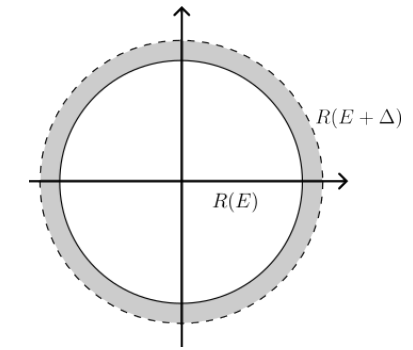
\includegraphics[width=0.4\linewidth]{Immagini/spazio delle fasi microcanonico (gas ideale).png}
    \caption{ensemble microcanonico di un gas ideale nello spazio delle fasi.}
    \label{fig: spazio delle fasi microcanonico (gas ideale)}
\end{figure}

Ora, per determinare l'area dell'ipersfera di raggio unitario si introduce l'integrale $D$-dimensionale $I_D$ invariante per rotazioni e proporzionale a $\hatA_{3N-1}$, dato da
\begin{equation}
\label{eq: integrale ID}
    \begin{split}
        I_D := \int d^Dx\,e^{-x^2} &= \bigg(\int_\R dx_1\cdots\int dx_D\bigg)e^{-(x_1^2 + \cdots + x_D^2)} \\
        &= \bigg(\int_\R dx\,e^{-x^2}\bigg)^D \\
        &= \pi^{D/2},
    \end{split}
\end{equation}
che in coordinate polari, sfruttando l'invarianza per rotazioni, diventa
\begin{equation}
\label{eq: integrale ID (coord. polari)}
    \begin{split}
        I_D = \int d\Omega_{D-1}\int_0^\infty dr\,r^{D-1}e^{-r^2} &= \hatA_{D-1}\frac{1}{2}\int_0^\infty dt\,t^{D/2 - 1}e^{-t} \\
        &= \hatA_{D-1}\frac{\Gamma(D/2)}{2},
    \end{split}
\end{equation}
dove si è posto $t = r^2$. Confrontando le due espressioni per $I_D$ \eqref{eq: integrale ID} e \eqref{eq: integrale ID (coord. polari)} segue che
\begin{equation}
    \hatA_{D-1} = \frac{2\pi^{D/2}}{\Gamma(D/2)}.
\end{equation}
Per determinare il volume dell'ensemble microcanonico nello spazio delle fasi si considera
\begin{equation}
    \begin{split}
        \vps(E,V,N) = \vps_q\vps_p &= V^N\hatA_{3N-1}R(E)^{3N-1}\frac{\p R}{\p E}\Delta \\
        &= V^N\frac{2\pi^{3N/2}}{\Gamma(3N/2)}(2mE)^{(3N-1)/2}\frac{\sqrt{2mE}}{E}\Delta \\
        &= \frac{(2\pi mV^{2/3}E)^{3N/2}}{\Gamma(3N/2)}\frac{\Delta}{E}.
    \end{split}
\end{equation}
Tuttavia, per trovare l'espressione dell'entropia è interessante il numero dei microstati $\Omega(E,V,N)$ disponibili. Per trovarlo, è necessario dividere il volume $\vps(E,V,N)$ per un'unità di misura arbitraria nello spazio delle fasi, la Meccanica quantistica suggerisce la seguente espressione
\begin{equation}
\label{eq: microstati complessivi gas ideale (microcanonico)}
    \Omega(E,V,N) = \frac{\vps(E,V,N)}{h^{3N}N!} = \bigg(\frac{2\pi m V^{2/3}E}{h^2}\bigg)^{3N/2}\frac{1}{N!\Gamma(3N/2)}\frac{\Delta}{E}.
\end{equation}
\begin{obs}
    L'uso della costante di Planck $h$ come unità fondamentale del volume nella \eqref{eq: microstati complessivi gas ideale (microcanonico)} è conseguenza del principio di indeterminazione di Heisenberg per le coordinate $\Delta q\Delta p \simeq h$; quindi $h$ rappresenta proprio il volume fondamentale nello spazio delle fasi che non avrebbe senso suddividere ulteriormente. Oltretutto, pensando di sostituire \eqref{eq: microstati complessivi gas ideale (microcanonico)} nella \eqref{eq: entropia (microcanonico)}, una ridefinizione di $h$ porta ad una ridefinizione additiva di $S$, conseguenza irrilevanti per i calcoli di differenze $\Delta S$.  
\end{obs}
\begin{obs}
    Il fattore di normalizzazione $N!$ nella \eqref{eq: microstati complessivi gas ideale (microcanonico)} è classicamente ingiustificato, ma la discussione quantistica lo prevede dandogli un significato molto importante e deriva dal fatto che particelle quantistiche identiche sono indistinguibili; pertanto, è necessario contare il numero di permutazione di queste ultime per evitare di ``contare'' tra le configurazioni possibili quelle che quantisticamente risultano indistinguibili. 
\end{obs}
Nel limite termodinamico, è possibile utilizzare l'approssimazione del logaritmo di Stirling
\begin{equation}
\label{eq: approssimazione stirling}
    \log{N!} \simeq N\log{(N)} - N.
\end{equation}
Dunque, dalla definizione di entropia microcanonica \eqref{eq: entropia (microcanonico)} si ottiene 
\begin{equation}
    S(E,V,N) = k\bigg[\log{\bigg(\frac{2\pi m V^{2/3}E}{h^2}\bigg)^{3N/2}} - \log{N!} - \log{\Gamma\bigg(\frac{3N}{2}\bigg) + \log{\frac{\Delta}{E}}}\bigg],
\end{equation}
che, usando l'approssimazione di Stirling e considerando il termine $\log{(\Delta/E)}$ soppresso nel limite termodinamico in modo da rimuovere ogni dipendenza da $\Delta$, si riduce alla formula di Sackur-Tetrode
\begin{equation}
\label{eq: formula scakur-tetrode entropia gas ideale (microcanonico)}
    S(E,V,N) = kN\log{\bigg[\frac{V}{N}\bigg(\frac{4\pi mE}{3Nh^2}\bigg)^{3N/2}}\bigg] + \frac{5}{2}kN.
\end{equation}
L'entropia determinata con la formula \eqref{eq: formula scakur-tetrode entropia gas ideale (microcanonico)} è, come ci si aspetta, estensiva nel limite termodinamico in quanto l'argomento del logaritmo è intensivo.
\begin{obs}
    Se non si avesse il fattore $1/N!$ nell'espressione \eqref{eq: microstati complessivi gas ideale (microcanonico)}, l'entropia mancherebbe del fattore $1/N$ nell'argomento del logaritmo che di conseguenza crescerebbe come $\ln{V} \simeq \ln{N}$; pertanto, l'entropia avrebbe un andamento del tipo $S \simeq kN\log{N}$, che nel limite termodinamico risulta più che estensivo, cioè cresce più rapidamente di $N$, e quindi non corretta.
\end{obs}
Avendo derivato dalla dinamica microscopica, ossia da $H(q,p)$, l'espressione dell'entropia, è possibile derivare le equazioni di stato del gas ideale nell'ensemble microcanonico. Queste sono
\begin{align}
    \frac{1}{T} &= \frac{\p S}{\p E}\bigg|_{V,N} = \frac{3kN}{2E},\quad(\mathrm{equazione\,di\,stato\,termica}), \\
    \frac{p}{T} &= \frac{\p S}{\p V}\bigg|_{E,N} = \frac{kN}{V},\quad(\mathrm{equazione\,di\,stato\,meccanica}), \\
    -\frac{\mu}{T} &= \frac{\p S}{\p N}\bigg|_{E,V} = -k\log{\bigg[\frac{V}{N}\bigg(\frac{4\pi mE}{3Nh^2}\bigg)^{3/2}\bigg]},\quad(\mathrm{equazione\,di\,stato\,chimica}),
\end{align}
da cui si possono ricavare le relazioni più familiari
\begin{equation}
    E = \frac{3}{2}kNT,\quad pV = kNT,
\end{equation}
dalle quali a loro volta si può dedurre che 
\begin{equation}
    p = \frac{2E}{3V}.
\end{equation}
Quest'ultima relazione è la conseguenza diretta del fatto che $S$ dipende solo dalla combinazione $V^{2/3}E$; infatti, per un processo adiabatico reversibile dove $S$ ed $N$ sono costanti, si ha che $V^{2/3}E = \mathrm{costante}$ e quindi 
\begin{equation}
    p = -\frac{\p E}{\p V}\bigg|_{S,N} = \frac{2E}{3V}.
\end{equation}
Combinando poi la $V^{2/3}E = \mathrm{costante}$ con $p = 2E/3V$ si ottiene che per un processo adiabatico reversibile vale
\begin{equation}
    pV^{5/3} = \mathrm{costante}.
\end{equation}

\section{Solido di Einstein nel microcanonico}
Uno dei modelli più semplici che si propone di descrivere i solidi tramite l'approccio quantistico è il modello del ``solido di Einstein''. Pur essendo molto semplice, storicamente ha coperto un ruolo di fondamentale importanza in quanto permetteva di mostrare come la Meccanica quantistica potesse spiegare l'andamento sperimentale del calore specifico dei solidi in funzione della temperatura, in particolare prevedeva che quest'ultimo tendesse a zero al diminuire della temperatura del solido, invece che essere costante come prevedeva la descrizione classica. 

Il modello di Einstein consiste nell'immaginare il solido come un insieme di $N$ atomi componenti un reticolo che possono oscillare intorno alle loro rispettive posizioni di equilibrio. L'ipotesi fondamentale del modello è che tutti i $3N$ modi normali di oscillazione del solido avessero tutti la stessa frequenza $\omega$. Anche se tale ipotesi non è affatto realistica, rende il modello incredibilmente semplice dal punto di vista analitico. Infatti, in questo modo il solido diventa equivalente all'insieme di $3N$ oscillatori armonici quantistici disaccoppiati di frequenza $\omega$. Un generico autostato nella base dell'energia può essere scritto come 
\begin{equation}
    \ket{\vn} = \ket{n_1} \otimes \cdots \otimes \ket{n_{3N}} \equiv \bigotimes_{a=1}^{3N}\ket{n_a},
\end{equation}
dove $\ket{n_a}$ è lo stato stazionario dell'$a$-esimo oscillatore di energia
\begin{equation}
    E_{n_a} = \hbar\omega\bigg(n_a + \frac{1}{2}\bigg).
\end{equation}
Dato che gli oscillatori sono disaccoppiati, l'energia totale del generico autostato è
\begin{equation}
    E_{\vn} \equiv E = \nsum_a E_{n_a} = \hbar\omega\bigg(n + \frac{3N}{2}\bigg),\quad n = \nsum_an_a.
\end{equation}
Quindi, c'è una degenerazione; infatti, una volta fissata l'energia $E$ nell'ensemble microcanonico ci sono più modi diversi per realizzare un microstato con questa energia. Si nota che:
\begin{enumerate}
    \item essendo i livelli discreti si può scegliere formalmente di porre $\Delta = 0$ e definire l'ensemble microcanonico per stati con esattamente energia $E$;
    \item fissare l'energia totale $E$ equivale a fissare $n = \nsum_an_a$.
\end{enumerate}
Pertanto, il numero di possibili microstati\footnote{La dipendenza da $V$ di $\Omega$ è omessa in quanto gli oscillatori hanno posizione fissata.} $\Omega(E,N)$ è dato da un conteggio combinatorio che restituisce i possibili insiemi $\{n_a\}$ tali che $n = \nsum_an_a$. Nella pratica, è come se si avessero $n$ quanti di energia da distribuire fra i $3N$ oscillatori in tutti i modi possibili, escluso in caso dell'energia di punto zero. Il problema si traduce quindi con il distribuire $n$ oggetti in $3N$ gruppi, pensando gli $n$ quanti come sfere, si hanno bisogno di $3N - 1$ divisori. Una tipica possibilità è mostrata in figura \ref{fig: solido di Einstein (microcanonico)}. Le possibilità distinte corrispondono a tutte le permutazione delle sfere e dei divisori, divise per le permutazioni delle sfere tra di loro e dei divisori tra di loro, in quanto queste sono equivalenti. Dunque, il numero di possibili microstati è dato da
\begin{equation}
    \Omega(E,N) = \frac{(n + 3N -1)!}{n!(3N - 1)!} = 
    \begin{pmatrix}
        n + 3N -1 \\
        n
    \end{pmatrix},
\end{equation}
dove i due fattori a denominatore servono proprio per evitare di contare le permutazioni equivalenti prima descritte. 
\begin{figure}[h]
    \centering
    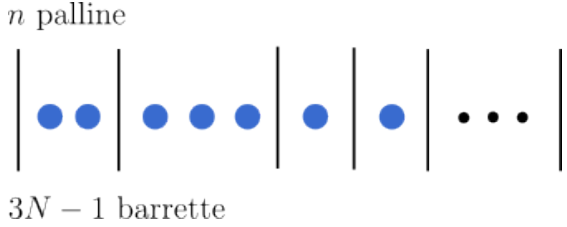
\includegraphics[width=0.5\linewidth]{Immagini/solido di Einstein (microcanonico).png}
    \caption{schema del problema combinatoriale per il solido di Einstein.}
    \label{fig: solido di Einstein (microcanonico)}
\end{figure}
Conoscendo $\Omega(E,N)$ si può determinare l'entropia con la definizione \eqref{eq: entropia (microcanonico)}
\begin{equation}
    S(E,N) = k\log{\frac{(n + 3N -1)!}{n!(3N - 1)!}},
\end{equation}
che nel limite termodinamico, usando l'approssimazione di Stirling \eqref{eq: approssimazione stirling} essendo $E$ ed $N$ molto grandi, diventa
\begin{equation}
    \begin{split}
        S(E,N) &\simeq k[(n + 3N)\log{(n + 3N)} - \cancel{(n + 3N)}  \\
        &- n\log{n} +\cancel{n} - 3N\log{3N} + \cancel{3N}] \\
        &= k[(n + 3N)\log{(n + 3N)} - n\log{n} - 3N\log{3N}]
    \end{split}
\end{equation}
Conoscendo adesso l'entropia si può ricavare la temperatura
\begin{equation}
\label{eq: entropia solido di Einstein (microcanonico)}
    \begin{split}
        \frac{1}{T} = \frac{\p S}{\p E}\bigg|_{N} = \frac{\p n}{\p E}\frac{\p S}{\p n}\bigg|_{N} = \frac{k}{\hbar\omega}[\log{(n + 3N)} - \log{n}] = \frac{k}{\hbar\omega}\log{\frac{n + 3N}{n}},
    \end{split}
\end{equation}
introducendo poi la quantità $\beta := 1/kT$ può essere riscritta come
\begin{equation}
    \beta\hbar\omega = \log{\frac{n + 3N}{n}},
\end{equation}
da cui si ricava la relazione tra il quanto di energia e l'energia del sistema
\begin{equation}
    n = \frac{3N}{e^{\beta\hbar\omega} - 1}.
\end{equation}
L'energia del sistema può quindi essere scritta in funzione di $\beta$, ossia della temperatura $T$, come
\begin{equation}
\label{eq: energia solido di Einstein (microcanonico)}
    E(T,N) = 3N\hbar\omega\bigg(\frac{1}{e^{\beta\hbar\omega} - 1} + \frac{1}{2}\bigg).
\end{equation}
Senza il quanto di energia, non si avrebbe avuto alcunché con cui confrontare $kT$ e quindi non si sarebbe potuto distinguere i limiti di alta e bassa temperatura. Questo è proprio il motivo per cui il problema non può essere affrontato classicamente. I due limiti in questione sono:
\begin{enumerate}
    \item ad alta temperatura, ossia per $kT \gg \hbar\omega$, la granulosità quantistica dell'energia è trascurabile ed, espandendo la \eqref{eq: energia solido di Einstein (microcanonico)}, si ha
    \begin{equation}
    \label{eq: energia solido di Einstein (alta T)}
        E(T,N) \simeq 3N\hbar\omega\bigg(\frac{1}{1 + \beta\hbar\omega + \dots - 1} + \frac{1}{2}\bigg) \simeq 3NkT,
    \end{equation}
    che coincide con il risultato classico, a meno del fattore additivo $1/2$, che non dipende da $\omega$;
    \item a bassa temperatura, ossia per $kT \ll \hbar\omega$, il comportamento del sistema è profondamente quantistico e la \eqref{eq: energia solido di Einstein (microcanonico)} si riduce a 
    \begin{equation}
    \label{eq: energia solido di Einstein (bassa T)}
        E(T,N) \simeq \frac{3N}{2}\hbar\omega + 3N\hbar\omega e^{-\beta\hbar\omega} + \cdots,
    \end{equation}
    dove il primo termine, ovvero l'energia di punto zero, è dominante, quindi tutti gli oscillatori in pratica sono nel loro stato fondamentale di energia $\hbar\omega/2$.
\end{enumerate}
La capacità termica ad $N$ fissato si ottiene da
\begin{equation}
    c_N = \frac{\p E}{\p T}\bigg|_N = \frac{\p \beta}{\p T}\frac{\p E}{\p \beta}\bigg|_N = 3Nk(\beta\hbar\omega)^2\frac{e^{\beta\hbar\omega}}{(e^{\hbar\beta\omega} - 1)^2},
\end{equation}
il cui andamento in funzione di $\beta$ è riportato nel grafico in figura \ref{fig: andamento cap. termica (solido di Einstein)}.
\begin{figure}[h]
    \centering
    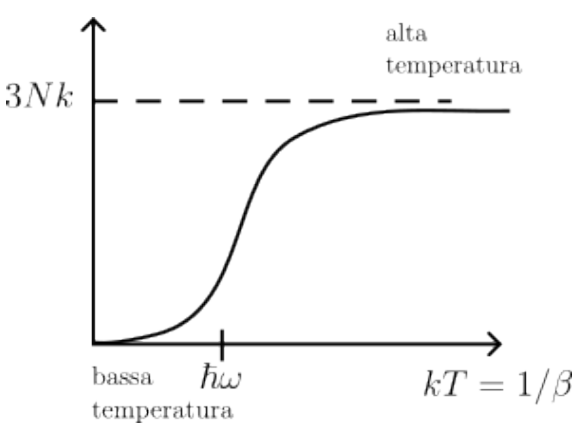
\includegraphics[width=0.4\linewidth]{Immagini/andamento cap. termica (solido di Einstein).png}
    \caption{andamento di $c_N$ in funzione di $\beta$ per il modello di Einstein.}
    \label{fig: andamento cap. termica (solido di Einstein)}
\end{figure}
Il comportamento classico ad alta temperatura si ritrova direttamente dalla \eqref{eq: energia solido di Einstein (alta T)}
\begin{equation}
    c_N \simeq 3Nk,\quad kT \gg \hbar\omega,
\end{equation}
mentre quello a bassa temperatura si ritrova dalla \eqref{eq: energia solido di Einstein (bassa T)} tenendo il primo termine esponenzialmente soppresso, dato che il termine dominante è indipendente da $T$
\begin{equation}
    \begin{split}
        c_N &= \frac{\p\beta}{\p T}\frac{\p}{\p\beta}\bigg(\frac{3N\hbar\omega}{2} + 3N\hbar\omega e^{-\beta\omega\hbar} + \cdots \bigg) \\
        &\simeq 3Nk(\beta\omega\hbar)^2e^{-\beta\omega\hbar},\quad kT \ll \hbar\omega.
    \end{split}
\end{equation}
Tuttavia, l'andamento di $c_N$ per $T \to 0$ non è in accordo con le osservazioni sperimentali, infatti la capacità termica dei solidi reali tende per $T \to 0$ tende a seguire leggi polinomiali; comunque, il modello di Einstein è sicuramente più accurato di quanto possa fare il modello classico, dove $c_N$ è indipendente dalla temperatura.

\subsection{Temperature negative}
Si consideri un sistema quantistico di $N$ componenti distinguibili e interagenti, in cui ognuno di essi abbia a disposizione solo due stati di energia $0$ ed $\epsilon$, come in figura \ref{fig: sistema a due livelli (T negative)}.
\begin{figure}[h]
    \centering
    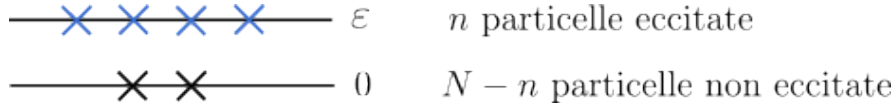
\includegraphics[width=0.7\linewidth]{Immagini/sistema a due livelli (T negative).png}
    \caption{esempio di sistema quantistico non interagente a due livelli.}
    \label{fig: sistema a due livelli (T negative)}
\end{figure}
Un generico microstato di energia $E$ è caratterizzato dal numero $n$ di componenti nel livello $\epsilon$, con gli altri $N - n$ nel livello $0$. L'energia totale del microstato allora è $E = n\epsilon$, da cui si osserva che $n$ determina direttamente $E$. Il numero di microstati $\Omega(E,N)$ con $E$ fissata corrisponde dato dal numero di modi di scegliere $n$ elementi tra le $N$ componenti a disposizione, per cui
\begin{equation}
    \Omega(E,N) = \frac{N!}{n!(N - n)!} =
    \begin{pmatrix}
        N \\
        n
    \end{pmatrix}.
\end{equation}
L'andamento di $\Omega(E,N)$ in funzione di $E$ segue una sorta di gaussiana con picco in $N/2$, come si vede in figura \ref{fig: andamento Omega e S (T negative)}; quindi, da un certo punto in poi $\Omega(E,N)$ decresce all'aumentare di $E$, a differenza di quasi tutti i sistemi.

Le conseguenze di questo comportamento si possono osservare calcolando l'entropia con la definizione \eqref{eq: entropia (microcanonico)} ottenendo
\begin{equation}
    S(E,N) = k\log{\frac{N!}{n!(N - n)!}},
\end{equation}
che nel limite termodinamico, usando l'approssimazione di Stirling dato che $E$ cresce con $N$ insieme a $n$, diventa
\begin{equation}
    S(E,N) = k[N\log{N} - n\log{n} - (N - n)\log{(N - n)}],
\end{equation}
il cui andamento in funzione di $E$ è mostrato in figura \ref{fig: andamento Omega e S (T negative)}. 
\begin{figure}[h]
    \centering
    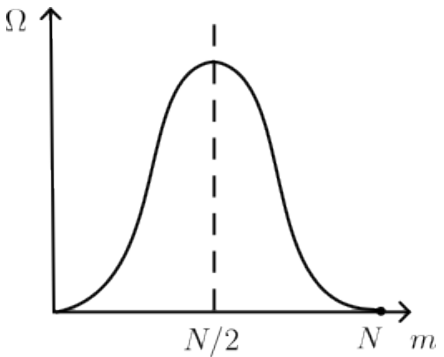
\includegraphics[width=0.36\linewidth]{Immagini/andamento di Omega (T negative).png}
    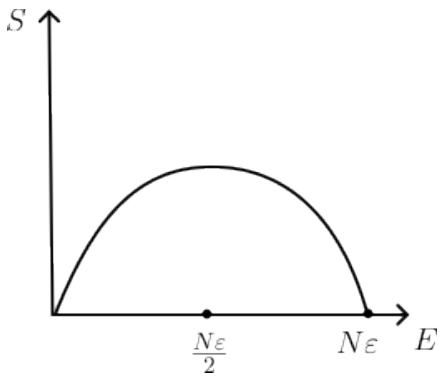
\includegraphics[width=0.35\linewidth]{Immagini/andamento entropia (T negative).png}
    \caption{andamento di: (i) $\Omega(E,N)$ in funzione di $N$; (ii) $S(E,N)$ in funzione dell'energia $E$ di un sistema quantistico non interagente a due livelli.}
    \label{fig: andamento Omega e S (T negative)}
\end{figure}
La particolarità è che $S$ non è una funzione crescente dell'energia, a differenza di quanto assunto normalmente in Termodinamica. A causa di ciò, deve necessariamente esistere una regione dove la temperatura è negativa. Questo accade perché all'aumentare dell'energia, il numero di stati a disposizione diminuisce; ad esempio, nello stato di massima energia esiste un solo modo per ordinare il sistema: tutte le particelle sono nello stato $\epsilon$. Per vedere questa anomalia, si usa l'equazione di stato termica \eqref{eq: equazioni di stato da S} da cui
\begin{equation}
\label{eq: temperature negative I}
    \frac{1}{T} = \frac{k}{\epsilon}\log{\frac{N - n}{n}} \quad\Rightarrow\quad \beta = \frac{1}{\epsilon}\log{\frac{N\epsilon - E}{E}},
\end{equation}
espressione che risulta diventare negativa per valori di energia $E > N\epsilon/2$. Osservando il grafico della funzione inversa, \ref{fig: andamento di beta e T  (T negative)}, si nota che la temperatura cresce fino a $E = N\epsilon/2$, in cui ha una singolarità, per poi cominciare a crescere asintoticamente da $-\infty$. 
\begin{figure}[h]
    \centering
    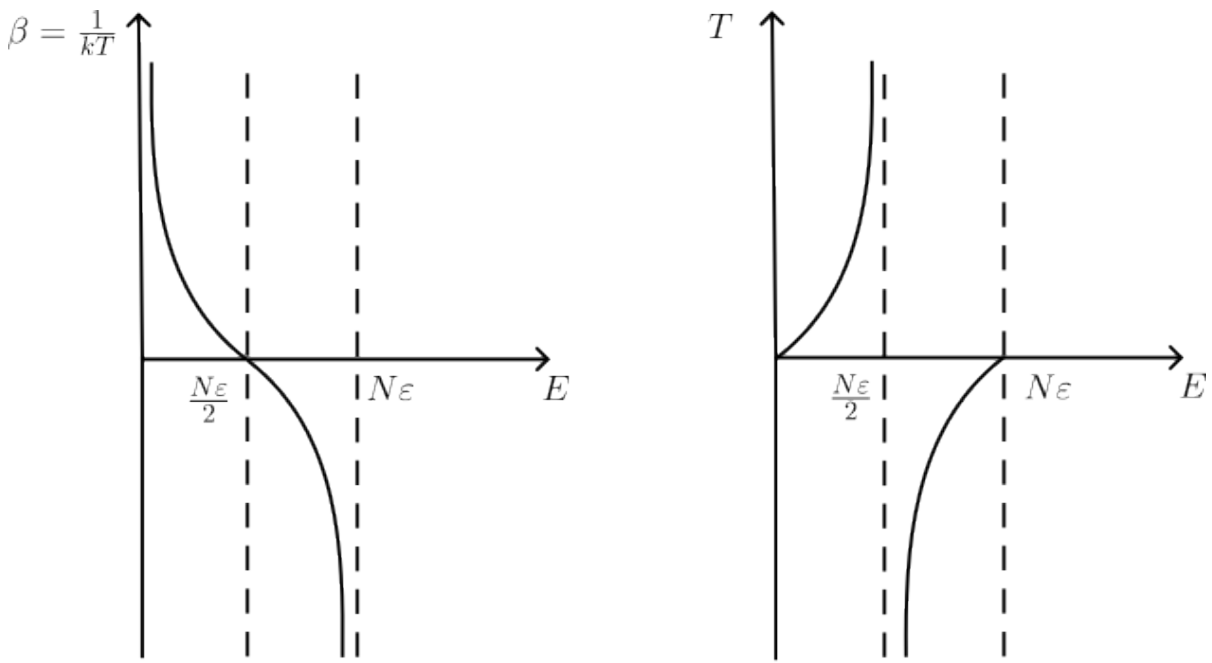
\includegraphics[width=0.7\linewidth]{Immagini/andamento di beta e T (T negative).png}
    \caption{andamento delle funzioni inverse: (i) $\beta(E)$; (ii) $T(E)$.}
    \label{fig: andamento di beta e T (T negative)}
\end{figure}
Quindi, in realtà nella regione in cui $T$ è negativa, la temperatura cresce con l'energia. La relazione \eqref{eq: temperature negative I} può essere invertita per avere
\begin{equation}
    E = \frac{N\epsilon}{1 + e^{\beta\epsilon}} \simeq 
    \begin{cases}
        0,\quad T \to 0^+ \\
        N\epsilon/2,\quad T \to \infty \\
        N\epsilon,\quad T \to 0^-
    \end{cases}
\end{equation}
Ovviamente non è semplice realizzare sperimentalmente dei sistemi che non abbiano altri livelli energetici oltre a $0$ ed $\epsilon$. Questi sistemi non dovrebbero avere nessuna possibilità di vibrare, di spostarsi o altro, altrimenti $\Omega(E)$ continuerebbe a crescere con $E$. Recentemente però sono stati condotti esperimenti con ``cold atoms'' che hanno osservato la presenza di temperature negative, in cui le particelle
si trovano in siti reticolari diversi, permettendo di mantenere la distinguibilità.

\subsection{Eigenvalue Thermalization Hypothesis}
Come detto in precedenza, per un sistema isolato in uno stato puro $\ket{\psi(t)}$, il valore di aspettazione di una generica osservabile $\vmedio{\hatO}_\psi$ non termalizza. L'azione di porsi nell'ensemble microcanonico corrisponde a selezionare gli autostati di energia con autovalori $E_n \in [E, E + \Delta]$, con $\Delta \ll E$. A partire dagli anni '90, si è mostrato che per quasi tutte le hamiltoniane di sistemi non integrabili a molte componenti, ossia per i corrispettivi quantistici dei sistemi ergodici classici, esistono importanti classi di osservabili che in effetti termalizzano. Tuttavia, si tratta solo di variabili locali, cioè definite solo per una sottoregione del sistema globale. Per gli operatori corrispondenti $\hatO$, gli elementi di matrice nella base dell'energia hanno la forma
\begin{equation}
    O_{mn} \simeq \mathcal{A}(E_n)\delta_{nm} + \Omega^{-1/2}\mathcal{A}_2(E_n,E_m)R_{mn},
\end{equation}
dove $\mathcal{A}$ è una funzione ``smoother'' e $R_{mn}$ è una matrice ``random'', estratta da una distribuzione gaussiana, dovuta al fatto che non si possono controllare i comportamenti delle altre particelle del sistema. La probabilità di transire da uno stato all'altro è soppressa dal fattore $\Omega^{-1/2}$. In tal caso, si trova che per quasi tutti i tempi $t$, il valore di aspettazione di $\hatO$ è uguale al valore medio all'equilibrio
\begin{equation}
    \vmedio{\hatO}_\psi = \vmedio{\hatO}_{EQ} \simeq \mathcal{A}(E),
\end{equation}
con una grandezza delle fluttuazioni relative dell'ordine $\Omega^{-1/2}$. Quindi, emerge un comportamento termodinamico per sottosistemi di un sistema quantistico isolato, che può essere espresso in termini della ``entropia di entanglement''. Dato che il sistema globale è in uno stato puro, descritto da $\hatrho(t) = \ket{\psi(t)}\bra{\psi(t)}$, la sua entropia di von Neumann \eqref{eq: definizione entropia von Neumann} è nulla e resta tale durante l'evoluzione del sistema. 

Si supponga ora di dividere i gradi di libertà del sistema in due sottosistemi disgiunti $A$ e $B$. Gli operatori densità relativi $\hatrho_A$ e $\hatrho_B$ si ottengono dalle tracce parziali sui gradi di libertà esterni al sottosistema, ovvero
\begin{equation}
    \hatrho_A = \Tr{\hatrho}_B,\quad \hatrho_B = \Tr{\hatrho}_A.
\end{equation}
Anche se $\hatrho$ corrisponde ad uno stato puro, $\hatrho_A$ e $\hatrho_B$ si riferiscono a stati misti nei due sottosistemi. Si può dimostrare che vale la disuguaglianza 
\begin{equation}
    |\SvN[\hatrho_A] - \SvN[\hatrho_B]| \le \SvN[\hatrho] \le \SvN[\hatrho_A] + \SvN[\hatrho_B],
\end{equation}
da cui, usando il fatto che $\SvN[\hatrho] = 0$ per uno stato puro, si ha
\begin{equation}
    \SvN[\hatrho_A] = \SvN[\hatrho_B] \ge 0.
\end{equation}
Le entropie parziali, o di entanglement, possono quindi crescere durante l'evoluzione del sistema fino a raggiungere il valore di equilibrio $\SvN[\hatrho_{AB}]$ dato da
\begin{equation}
    \SvN[\hatrho_{AB}] \equiv \SvN[\hatrho_A] = \SvN[\hatrho_B].
\end{equation}
La possibilità che le entropie dei due sottosistemi crescano, pur rimanendo nulla l'entropia del sistema globale, appare paradossale.  L'informazione quantistica iniziale, quindi la conoscenza esatta dello stato, non è sparita, ma è accessibile solo tramite misure ``globali'' che non termalizzano. In pratica, il sistema nel suo complesso gioca il ruolo di bagno termico per i sottosistemi.

\chapter{Ensemble canonico}
Se al posto dell'energia interna si controlla la temperatura del sistema, allora l'ensemble che descrive il sistema è l'ensemble canonico. Il principale motivo per usare questo ensemble piuttosto che il microcanonico è semplicemente che la temperatura $T$ è nettamente più semplice da controllare e misurare rispetto all'energia $E$.
\begin{figure}[h]
    \centering
    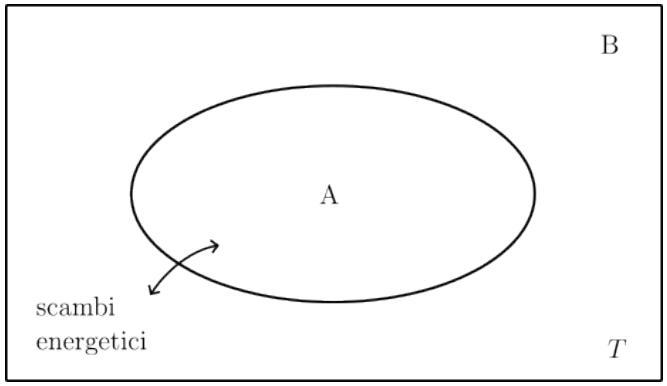
\includegraphics[width=0.45\linewidth]{Immagini/sistema generico (canonico).png}
    \caption{sistema generico per l'ensemble canonico.}
    \label{fig: sistema generico (canonico)}
\end{figure}
Si consideri, in riferimento alla figura \ref{fig: sistema generico (canonico)}, un sottosistema $A$ posto a contatto termico con un termostato $B$, ossia un sistema avente capacità termica molto maggiore di quella di $A$, in modo che quando viene stabilito l'equilibrio termico tra $A$ e $B$ questo avvenga alla temperatura di $B$. Essenzialmente, impostando la temperatura di $B$ si ha la certezza che $A$ prima o poi raggiungere tale temperatura. Sia ora $E$ l'energia totale del sistema, data dalla somma $E = E_A + E_B$. Per il sistema complessivo, nel caso microcanonico, i microstati sono tutti equiprobabili e il loro numero è dato da $\Omega(E)$. Si supponga adesso che $A$ sia in un microstato $\nu$ con energia $E_\nu$, di conseguenza $B$ può trovarsi in un qualsiasi stato purché abbia energia $E - E_\nu$, pertanto il numero di tali microstati è $\Omega_B(E - E_\nu)$. Siccome i microstati sono tutti equiprobabili, la probabilità che il microstato complessivo sia nello stato appena descritto è data da
\begin{equation}
    P(\nu) = \frac{\Omega_B(E - E_\nu)}{\Omega(E)}.
\end{equation}
Quindi, fissando $E_\nu$ risultano accettabili tutti gli stati di $B$ con energia complementare. 
\begin{obs}
    In linea di principio, a causa delle fluttuazioni avere energia alta in $A$, ma con la condizione che quella in $B$ sia bassa, e questo accade in pochi casi; pertanto, questi casi possono essere trascurati e ci si aspetta che la probabilità non sia uguale per tutte le energie.
\end{obs}
Dunque, trascurando $\Omega(E)$ dato che si tratta di una normalizzazione indipendente da $\nu$, si ha
\begin{equation}
    P(\nu) \propto \Omega_B(E - E_\nu) = \exp{[\log{\Omega_B(E - E_\nu)}]}.
\end{equation}
Consistentemente con l'ipotesi che $B$ abbia una capacità termica molto maggiore di quella di $A$, si può assumere che $E \gg E_\nu$, così facendo si può espandere il logaritmo in serie di Taylor ottenendo
\begin{equation}
    \log{\Omega_B(E - E_\nu)} = \log{\Omega_B(E)} - \frac{\p}{\p E}(\log{\Omega_B})E_\nu + \cdots,
\end{equation}
da cui, usando l'entropia di Boltzmann \eqref{eq: entropia (microcanonico)} e l'equazione di stato termica \eqref{eq: equazioni di stato da S}, si ha
\begin{equation}
    \frac{\p}{\p E}(\log{\Omega_B}) = \frac{1}{k}\frac{\p S_B}{\p E} = \frac{1}{kT_B} \equiv \beta_B,
\end{equation}
dove $T_B$ è la temperatura di $B$ che all'equilibrio coincide con quella di $A$. Dunque, la probabilità $P(\nu)$ risulta essere
\begin{equation}
    P(\nu) \propto e^{-\beta E_\nu},
\end{equation}
dove $e^{-\beta E_\nu}$ è tipicamente chiamato ``fattore di Boltzmann''. Ricapitolando, la probabilità che il microstato complessivo sia nello stato in questione è determinata a partire da $B$, ma all'equilibrio, a meno di una costante di normalizzazione, è la stessa del sistema $A$. Introducendo ora la costante di normalizzazione $Z$ in modo che 
\begin{equation}
\label{eq: probabilità microstati (canonico)}
    P(\nu) = \frac{e^{-\beta E_\nu}}{Z},
\end{equation}
dalla normalizzazione di $P(\nu)$ impone che $\nsum_\nu P(\nu) = 1$ segue che
\begin{equation}
\label{eq: funzione di partizione (canonico)}
    Z = \nsum_\nu e^{-\beta E_\nu}.
\end{equation}
In generale, la quantità $Z(T,V,N,\dots)$ è detta ``funzione di partizione'' del sistema ed è proprio la funzione che conferma il fatto che nell'ensemble canonico i microstati non sono più tutti equiprobabili: microstati con energia molto più grande rispetto all'energia termica $kT$ sono esponenzialmente soppressi.

\subsubsection{Fluttuazioni dell'energia}
Si consideri un sistema descrivibile tramite l'ensemble canonico, nel limite termodinamico il sottosistema $A$ ha un energia $E_A$ fissata, a meno di fluttuazioni trascurabili delle energie $E_\nu$ dei singoli microstati, che per consistenza deve corrispondere al valor medio delle energie $E_\nu$ dato da
\begin{equation}
\label{eq: valor medio E (canonico)}
    \begin{split}
        \vmedio{E} = \nsum_\nu P(\nu)E_\nu &= \frac{1}{Z}\nsum_\nu E_\nu e^{-\beta E_\nu} \\
        &= -\frac{1}{Z}\frac{\p}{\p\beta}\nsum_\nu e^{-\beta E_\nu} \\
        &= -\frac{\p}{\p\beta}\log{Z}.
    \end{split}
\end{equation}
Quando le variabili di controllo sono $\{T,V,N\}$, il potenziale termodinamico corretto è l'energia libera di Helmoltz $F$, per cui $Z \equiv Z(T,V,N) = e^{-\beta F(T,V,N)}$, dove si è introdotta
\begin{equation}
    F = -\frac{\log{Z}}{\beta}.
\end{equation}
Tramite $F$ è possibile riscrivere \eqref{eq: valor medio E (canonico)} come
\begin{equation}
    \vmedio{E} = \frac{\p}{\p\beta}(\beta F) = F + \beta\frac{\p F}{\p\beta} = F - T\frac{\p F}{\p T},
\end{equation}
dove si è usata la relazione
\begin{equation}
    \beta\frac{\p}{\p\beta} = \frac{\p}{\p(\log{\beta})} = -\frac{\p}{\p(\log{T})} = -T\frac{\p}{\p T},\quad \beta = \frac{1}{kT}.
\end{equation}
Il fatto che $F$ sia proprio l'energia libera di Helmoltz è confermato ricordando l'equazione di stato \eqref{eq: equazioni di stato da F} relativa all'entropia, da cui si ricava la trasformata di Legendre che lega i due potenziali
\begin{equation}
    F = \vmedio{E} -TS.
\end{equation}
Fino ad ora si sono assunte trascurabili le fluttuazioni rispetto al valore medio nel limite termodinamico, anche se l'energia dei microstati $E_\nu$ non è fissata. L'energia termodinamica è ben definita e non si osservano fluttuazioni spontanee rilevanti nel suo valore; tuttavia, questa affermazione deve seguire automaticamente dalla trattazione canonica. Per vederlo, si definisce la fluttuazione di energia come $\delta E = E - \vmedio{E}$, dove $E$ è il valore dell'energia misurata per il sottosistema $A$, il quale deve risultare nullo, ossia $\delta E = 0$. La quantità rilevante è la varianza $\sigma_E^2$ delle fluttuazioni data da
\begin{equation}
    \sigma^2_E := \bigvmedio{(\delta E)^2} = \vmedio{E^2} - \vmedio{E}^2.
\end{equation}
Dalla \eqref{eq: valor medio E (canonico)}, si deduce che
\begin{equation}
    \vmedio{E^2} = \nsum_\nu P(\nu)E_\nu^2 = \frac{1}{Z}\nsum_\nu E_\nu^2 e^{-\beta E_\nu} = \frac{1}{Z}\frac{\p^2Z}{\p\beta^2},
\end{equation}
considerando quindi la quantità
\begin{equation}
    \frac{\p\vmedio{E}}{\p\beta} = -\frac{\p}{\p\beta}\bigg(\frac{1}{Z}\frac{\p Z}{\p\beta}\bigg) = \frac{1}{Z^2}\bigg(\frac{\p Z}{\p\beta}\bigg)^2 - \frac{1}{Z}\frac{\p^2Z}{\p\beta^2} \equiv \vmedio{E}^2 - \vmedio{E^2},
\end{equation}
si trova che
\begin{equation}
\label{eq: varianza di E (canonico)}
    \sigma_E^2 = - \frac{\p\vmedio{E}}{\p\beta}.
\end{equation}
Dato che $\vmedio{E}$ è una quantità estensiva, mentre $\beta T$ è intensiva, allora $\sigma^2_E$ è anch'essa estensiva; in particolare, si ha
\begin{equation}
    \sigma_E^2 \simeq N,\quad N\to\infty.
\end{equation}
Quindi, le fluttuazioni relative di energia nel limite termodinamico si comportano come
\begin{equation}
\label{eq: andamento fluttuazioni di E (canonico)}
    \frac{\sigma}{\vmedio{E}} \simeq \frac{\sqrt{N}}{N} = \frac{1}{\sqrt{N}}.
\end{equation}
Dunque, l'assunzione che le fluttuazioni di energia siano trascurabili nel limite termodinamico è giustificata dall'andamento \eqref{eq: andamento fluttuazioni di E (canonico)} di queste ultime in funzione di $N$.
\begin{obs}
    Si nota che l'equazione \eqref{eq: varianza di E (canonico)} connette la varianza $\sigma^2_E$ alle funzioni di risposta $c_{V,N}$; infatti
    \begin{equation}
    \label{eq: relazione tra le fluttuazioni di E e cV,N (canonico)}
        \frac{\p\vmedio{E}}{\p\beta} = \frac{\p T}{\p\beta}\frac{\p\vmedio{E}}{\p T} = -kT^2\frac{\p E}{\p T} = -kT^2c_{V,N} = -\sigma_E^2.
    \end{equation}
    Questo è un esempio del ``fluctuation dissipation theorem'', il quale collega le fluttuazioni all'equilibrio con la risposta del sistema alla variazione di parametri di controllo e a fenomeni di dissipazione quando si è fuori equilibrio.
\end{obs}

\subsubsection{Ensemble canonico quantistico}
Nel limite classico spesso i livelli di energia sono continui e tipicamente la somma sui microstati diventa un integrale sullo spazio delle fasi, passando così dal discreto al continuo. Nel contesto quantistico, nella base dell'energia, la matrice densità $\rho$ è diagonale e su di essa sono presenti le probabilità $P(\nu)$ dei singoli microstati, quindi
\begin{equation}
    \rho_{\mu\nu} = P(\nu)\delta_{\mu\nu},\quad P(\nu) = \frac{e^{-\beta E_\nu}}{Z}.
\end{equation}
In una base qualsiasi, l'operatore densità $\hatrho$ è dato da
\begin{equation}
    \hatrho = \frac{e^{-\beta\hatH}}{Z},\quad Z = \Tr{e^{-\beta\hatH}},
\end{equation}
dove $Z$ corrisponde alla normalizzazione per avere $\Tr{\hatrho} = 1$. Pertanto, il valore di aspettazione $\vmedio{\hatO}$ di un'osservabile $O$ rappresentata dal corrispettivo operatore autoaggiunto $\hatO$ è dato dal rapporto
\begin{equation}
    \vmedio{\hatO} = \frac{\Tr{\hatO e^{-\beta\hatH}}}{Z} = \frac{\Tr{\hatO e^{-\beta\hatH}}}{\Tr{e^{-\beta\hatH}}}.
\end{equation}

\section{Entropia di Gibbs}
Fino ad ora si è derivata la forma della probabilità $P(\nu)$ tramite assunzioni ad hoc sia per l'ensemble microcanonico che per il canonico. Tuttavia, esiste una formulazione generale, dovuta a Gibbs, che permette di trovare l'espressione del funzione di entropia per un qualsiasi ensemble
\begin{equation}
\label{eq: definizione entropia Gibbs}
    \SG[P(\nu)] = -k\nsum_\nu P(\nu)\log{P(\nu)} = -k\vmedio{\log{P(\nu)}}.
\end{equation}
In altre parole, è possibile derivare la statistica dell'equilibrio tramite un'espressione generale dell'entropia\footnote{L'espressione \eqref{eq: definizione entropia Gibbs} è supposta valere anche fuori equilibrio.}, data dalla \eqref{eq: definizione entropia Gibbs}, definita come un funzionale delle possibili forme funzionali della probabilità all'equilibrio. Siccome per condizioni esterne fissate l'equilibrio viene raggiunto al massimo dell'entropia, ciò implica che tra le possibili probabilità $P(\nu)$ vengono selezionate proprio quelle che massimizzano l'entropia. Pertanto, si può determinare la probabilità all'equilibrio massimizzando il funzionale \eqref{eq: definizione entropia Gibbs} e tenendo conto degli eventuali vincoli.

Come prima cosa, si deve verificare che l'entropia $\SG$ sia una quantità estensiva. Perciò, si considerano due sottosistemi indipendenti $A$ e $B$, componenti di un sistema complessivo $A\cup B$. La probabilità congiunta, data l'indipendenza di $A$ e $B$, è data da 
\begin{equation}
    P_{AB}(\nu_A,\nu_B) = P_A(\nu_A)P_B(\nu_B).
\end{equation}
Utilizzando adesso le proprietà dei logaritmi e le condizioni di normalizzazione per le probabilità $\nsum_{\nu_A}P_A$ e $\nsum_{\nu_B}P_B$ si ottiene
\begin{equation}
    \begin{split}
        \SG_{AB} &= -k\nsum_{\nu_A}\nsum_{\nu_B}P_{AB}(\nu_A,\nu_B)\log{ P_{AB}(\nu_A,\nu_B)} \\
        &= -k\nsum_{\nu_A}\nsum_{\nu_B}P_A(\nu_A)P_B(\nu_B)[\log{P_A(\nu_A)} + \log{P_B(\nu_B)}] \\
        &=-k\nsum_AP_A(\nu_A)\log{P_A(\nu_A)}\nsum_{\nu_B}P_B(\nu_B) \\
        &-k\nsum_{\nu_B}P_B(\nu_B)\log{P_B(\nu_B)}\nsum_{\nu_A}P_A(\nu_A) \\
        &\equiv \SG_A + \SG_B.
    \end{split}
\end{equation}
Nel limite classico, l'entropia di Gibbs $\SG$ si riduce alla formula di Boltzmann
\begin{equation}
    \SG = -k\sum_{\nu = 1}^\Omega\frac{1}{\Omega}\log{\frac{1}{\Omega}} = k\log{\Omega} \equiv S;
\end{equation}
invece, nel contesto quantistico, $\SG$ si può riscrivere come
\begin{equation}
    \SG[\hatrho] = -k\Tr{\hatrho\log{\hatrho}} = k\SvN,
\end{equation}
che corrisponde, a meno di una costante moltiplicativa, all'entropia di von Neumann \eqref{eq: definizione entropia von Neumann}, connettendo così l'entropia termodinamica alla quantità di informazione contenuta in un sistema quantistico.

\subsubsection{Derivazione di \texorpdfstring{$\bm{P(\nu)}$}{P(nu)} nell'ensemble microcanonico}
Sempre nel limite classico, è possibile derivare la forma di $P(\nu)$ massimizzando il funzionale $\SG[P(\nu)]$ rispetto a $P(\nu)$ tenendo del vincolo $\nsum_\nu P(\nu) = 1$. Per farlo, si utilizza la tecnica dei moltiplicatori di Lagrange, in questo caso si ha
\begin{equation}
    \tilde{\SG}[P] = \SG[P] + \alpha_0\bigg(\nsum_\nu P(\nu) - 1\bigg),
\end{equation}
la cui variazione deve risultare nulla rispetto ad una variazione $\delta P(\nu)$ arbitraria
\begin{equation}
    \begin{split}
        0 \equiv \delta\tilde{\SG}[P] &= \delta\bigg(-k\nsum_\nu P(\nu)\log{P(\nu)} + \alpha_0\nsum_\nu P(\nu)\bigg)  \\
        &= \nsum_\nu\delta P(\nu)\bigg(-k\log{P(\nu)} - k + \alpha_0\bigg),
    \end{split}
\end{equation}
dove essendo la variazione in $P(\nu)$ arbitraria, necessariamente il termine nella parentesi tonda deve annullarsi per soddisfare la condizione di massimizzazione, per cui
\begin{equation}
    P(\nu) = e^{-1 + \alpha_0/k}.
\end{equation}
Imponendo ora il vincolo $\nsum_\nu P(\nu) = 1$ si ottiene
\begin{equation}
    \Omega e^{-1 + \alpha_0/k} = 1\quad\Rightarrow\quad P(\nu) = \Omega^{-1},
\end{equation}
che è esattamente il risultato trovato nella \eqref{eq: probabilità microstati (microcanonico)}.

\subsubsection{Derivazione di \texorpdfstring{$\bm{P(\nu)}$}{P(nu)} nell'ensemble canonico}
Come già detto, nell'ensemble canonico i microstati $\nu$ non hanno tutti la stessa energia, tuttavia all'equilibrio si ha un'energia termodinamica complessiva pari a
\begin{equation}
    E \equiv \vmedio{E} = \nsum_\nu E_\nu P(\nu).
\end{equation}
Si deve fare attenzione che ora si hanno due vincoli, corrispondenti proprio a
\begin{equation}
    \nsum_\nu P(\nu) = 1,\quad \nsum_\nu P(\nu)E_\nu = E.
\end{equation}
Dato il numero di vincoli, sono necessari due moltiplicatori di Lagrange, per cui
\begin{equation}
    \tilde{\SG}[P] = \SG[P] + \alpha_0\bigg(\nsum_\nu P(\nu) - 1\bigg) + \alpha_E\bigg(\nsum_\nu P(\nu)E_\nu - E\bigg).
\end{equation}
In modo analogo a quanto fatto per l'ensemble microcanonico, si massimizza il funzionale di entropia ponendo $\delta\tilde{\SG}[P] = 0$ rispetto ad una $\delta P(\nu)$ arbitraria. Si pone quindi
\begin{equation}
    \begin{split}
        0 \equiv \delta\tilde{\SG}[P] &= \delta\bigg(-k\nsum_\nu P(\nu)\log{P(\nu)} + \alpha_0\nsum_\nu P(\nu) + \alpha_E\nsum_\nu P(\nu)E_\nu\bigg) \\
        &= \nsum_\nu \delta P(\nu)(-k\log{P(\nu)} - k + \alpha_0 + \alpha_E E_\nu),
    \end{split}
\end{equation}
il quale si annulla se e solo se il termine nella parentesi tonda è nullo, per cui si ha
\begin{equation}
    P(\nu) = e^{-1 + \alpha_0/k}e^{\alpha_E E_\nu/k}.
\end{equation}
Imponendo il vincolo di normalizzazione si fissa il moltiplicatore $\alpha_0$
\begin{equation}
    \nsum_\nu P(\nu) = \nsum_\nu e^{-1 + \alpha_0/k}e^{\alpha_E E_\nu/k} = 1\quad\Rightarrow\quad Z = \nsum_\nu e^{\alpha_E E_\nu/k};
\end{equation}
per imporre invece il secondo vincolo, tenendo conto della condizione di normalizzazione $Z = \nsum_\nu e^{\alpha_E E_\nu/k}$ appena trovata, si riscrive l'entropia come
\begin{equation}
    \begin{split}
        \SG = -k\nsum_\nu P(\nu)\log{P(\nu)} &= -k\nsum_\nu P(\nu)\bigg(\frac{\alpha_E}{k}E_\nu - \log{Z}\bigg) \\
        &= -\alpha_E\vmedio{E} + k\log{Z},
    \end{split}
\end{equation}
da cui, confrontandola con l'equazione di stato termica \eqref{eq: equazioni di stato da S} e identificando $E \equiv \vmedio{E}$, segue che
\begin{equation}
    \alpha_E \equiv -\frac{1}{T}.
\end{equation}
Dunque, la probabilità $P(\nu)$ risulta essere
\begin{equation}
    P(\nu) = \frac{e^{-E_\nu/kT}}{Z} = \frac{e^{-\beta E_\nu}}{Z},\quad Z = \nsum_\nu e^{-\beta E_\nu}.
\end{equation}
che coincide proprio con il risultato trovato nella \eqref{eq: probabilità microstati (canonico)}. Tornando infine all'espressione dell'entropia $\SG = \alpha_E\vmedio{E} + k\log{Z}$, sostituendo $\alpha_E = 1/T$ e $\vmedio{E} \equiv E$, si ha
\begin{equation}
    \SG = \frac{E}{T} + k\log{Z}\quad\Rightarrow\quad TS = E + \frac{\log{Z}}{\beta},
\end{equation}
la quale confrontata con $F = E - TS$ restituisce 
\begin{equation}
    F = -\frac{\log{Z}}{\beta}\quad\Rightarrow\quad Z = e^{-\beta F}.
\end{equation}

\section{Legame tra microcanonico e canonico}
Nell'ensemble canonico la termodinamica è derivata a partire dalla funzione di partizione $Z \equiv Z(T,V,N)$ definita dalla \eqref{eq: funzione di partizione (canonico)}, dove tutti i microstati $\nu$ con la medesima energia contribuiscono allo stesso modo. Indicando con $\Omega(E_e,V,N)$ il numero di microstati $\nu_e$ con una data energia $E_e$, si può scrivere
\begin{equation}
    Z(T,V,N) = \nsum_e\sum_{\nu_e = 1}^{\Omega(E_e)} e^{-\beta E_e} = \nsum_e\Omega(E_e)e^{-\beta E_e},
\end{equation}
dove $\Omega(E_e)$ rappresenta la ``degenerazione'' dell'energia $E_e$. Dato che per sistemi macroscopici classici le energie possibili formano un continuo, e che anche per sistemi macroscopici quantistici i livelli sono estremamente densi, è conveniente introdurre un fattore di densità di probabilità $P(E)$ che dipende solo dall'energia. In questo modo, $P(E)dE$ rappresenta la probabilità che il sistema si trovi in un microstato di energia compresa nell'intervallo di energia $(E, E + dE)$. In termini della densità di microstati $g(E)$, definita come
\begin{equation}
\label{eq: definizione g(E) (microcanonico)}
    g(E)\,dE = \Omega(E)|_{\Delta = dE},
\end{equation}
dove $\Omega(E)$ è il numero di microstati in una corona di spessore infinitesimo $dE$ intorno al livello di energia, si ha
\begin{equation}
\label{eq: P(E) in termini di g(E) (canonico)}
    P(E)\,dE = \frac{e^{-\beta E}}{Z}g(E)\,dE,\quad Z(\beta) = \int_0^\infty dE\,g(E)e^{-\beta E}.
\end{equation}
\begin{notz}
    Per semplicità, nel seguito si omette la dipendenza dalle variabili $\{V,N\}$ e si indica la dipendenza dalla temperatura $T$ tramite $\beta$.
\end{notz}
Se si è nel caso in cui $\beta > 0$, come normalmente accade, l'espressione della funzione di partizione nella \eqref{eq: P(E) in termini di g(E) (canonico)} coincide con la trasformata di Laplace della densità di microstati $g(E)$; pertanto, l'equazione può essere invertita ottenendo
\begin{equation}
\label{eq: g(E) in termini di Z(beta) (canonico)}
    g(E) = \frac{1}{2\pi i}\int_\Gamma d\beta\,e^{\beta E}Z(\beta),\quad \beta = \beta_1 + i\beta_2,\,\beta_2 \in \R,\,\Gamma \in \C_\beta,
\end{equation}
dove il cammino di integrazione $\Gamma$ può essere deformato arbitrariamente fintanto che l'integrale converge e non si incontrano singolarità. Per verificare che quest'ultima è effettivamente la formula inversa, si può sostituire la \eqref{eq: P(E) in termini di g(E) (canonico)} nella \eqref{eq: g(E) in termini di Z(beta) (canonico)} ottenendo proprio
\begin{equation}
    \begin{split}
        g(E) &= \frac{1}{2\pi}\int_\R d\beta_2\int_0^\infty dE'\,g(E')e^{-i(\beta_1 + i\beta_2)(E' - E)} \\
        &= \int_0^\infty dE'\,g(E')e^{-\beta_1(E' - E)}\frac{1}{2\pi}\int_\R d\beta_2\,e^{i\beta_2(E' - E)} \\
        &= \int_0^\infty dE'\,g(E')e^{-\beta_1(E' - E)}\delta(E' - E) \\
        &\equiv g(E),
    \end{split}
\end{equation}
dove si è sfruttato il fattore $e^{-\beta_1 E'}$ per invertire l'ordine di integrazione. Quindi, tornando alla \eqref{eq: P(E) in termini di g(E) (canonico)}, nel limite termodinamico si ha
\begin{equation}
\label{eq: definizione g(E) limite TD (microcanonico)}
    g(E)\,dE = \Omega(E)|_\Delta = e^{S(E)/k} \simeq \Omega(E)|_\Delta = g(E) \Delta,\quad \forall\Delta \ll E,
\end{equation}
dove appunto la scelta di $\Delta$ è irrilevante in quanto quantità non estensiva; mentre, il membro di sinistra nel limite termodinamico è
\begin{equation}
    Z(\beta) = e^{-\beta F(\beta)},
\end{equation}
dove $S(E)$ e $F(T)$ sono proprio l'entropia e l'energia libera di Helmholtz, espresse rispettivamente tramite l'ensemble microcanonico e canonico. L'espressione \eqref{eq: P(E) in termini di g(E) (canonico)}, nel limite termodinamico, diventa
\begin{equation}
\label{eq: P(E) in termini di g(E) limite TD (canonico)}
    e^{-F(\beta)/kT} = \frac{1}{\Delta}\int_0^\infty dE\, e^{(S - E/T)/k} \equiv \frac{1}{\Delta}\int_0^\infty dE\, e^{-f(E)},
\end{equation}
dove $E$ non è l'energia termodinamica ma una generica variabile di integrazione. Tuttavia, l'integrale a secondo membro può essere valutato con il metodo del ``punto a sella''. Il massimo dell'esponente si ha per 
\begin{equation}
    \frac{\p f}{\p E} = \frac{\p}{\p E}\bigg(-S + \frac{E}{T}\bigg) = 0\quad\Longleftrightarrow\quad \frac{\p S}{\p E} = \frac{1}{T},
\end{equation}
ossia quando l'energia $E$ coincide proprio con l'energia termodinamica $\vmedio{E}$ del sistema canonico a temperatura $T$. Quindi, il valore medio $\vmedio{E}$ rappresenta anche il valore di $E$ che massimizza la densità di probabilità $P(E)$, ossia il ``valore più probabile''. Tornando all'integrale, questo può essere valutato tramite la formula
\begin{equation}
    \begin{split}
        \frac{1}{\Delta} \int_{0}^{\infty} dE \, e^{-f(E)} &= e^{-f(\langle E \rangle)}\bigg( \frac{1}{\Delta} \sqrt{\frac{2\pi}{f''(\langle E \rangle)}} + \cdots \bigg) \\
        &= \exp\bigg[{-f(\langle E \rangle) - \frac{1}{2} \log \frac{\Delta^2 f''(\langle E \rangle)}{2\pi}} + \cdots\bigg],
    \end{split}
\end{equation}
dato che $f(E)$ è estensiva e scala con $N$, e $f''(E)$ scala con $1/N$. Quindi, il secondo termine nell'esponenziale scala con $\log{N}$ ed è pertanto trascurabile rispetto al primo termine. Il risultato è che l'espressione \eqref{eq: P(E) in termini di g(E) limite TD (canonico)} si riduce a
\begin{equation}
    e^{-F/kT} = e^{[S(\vmedio{E}) - \vmedio{E}/T]/k},
\end{equation}
da cui si ricava nuovamente la trasformata di Legendre che lega $F$ a $\vmedio{E}$ tramite
\begin{equation}
    F = \vmedio{E} - TS.
\end{equation}
Dunque, tale trasformata di Legendre è l'approssimazione termodinamica alla trasformata di Laplace \eqref{eq: P(E) in termini di g(E) (canonico)} che lega la funzione di partizione $Z(\beta)$ alla densità di microstati $g(E)$.

\subsubsection{Trattamento canonico di sistemi non interagenti}
Si consideri un sistema composto di $N$ componenti distinguibili e non interagenti. Un microstato $\nu$ del sistema complessivo corrisponde ad una collezione di microstati $\nu_i$, con $i = 1,\dots,N$, dei vari componenti. L'energia del microstato $\nu$, data l'assenza di interazioni è
\begin{equation}
\label{eq: energia sistema non interagente (canonico)}
    E_\nu = \nsum_iE_{\nu_i}.
\end{equation}
Di conseguenza, la funzione di partizione si fattorizza in quelle di ciascun componente
\begin{equation}
\label{eq: funzione di partizione sistemi non interagenti (canonico)}
    \begin{split}
        Z = \nsum_\nu e^{-\beta E_\nu} &= \nsum_{\nu_1}\cdots\nsum_{\nu_N}e^{-\beta(E_{\nu_1} + \cdots E_{\nu_N})} \\
        &= \nsum_{\nu_1}e^{-\beta E_{\nu_1}}\cdots \nsum_{\nu_N}e^{-\beta E_{\nu_N}} \\
        &= \nprod_iZ_{(i)}.
    \end{split}
\end{equation}
\begin{obs}
    I sistemi reali sono ovviamente sempre interagenti, tuttavia l'approssimazione non interagente può essere valida per i gas in regimi di bassa densità.
\end{obs}
Essendo i componenti identici, secondo la Meccanica quantistica sono anche indistinguibili e la necessità di simmetrizzazione, o antisimmetrizzazione, rispetto ai loro scambi introduce una sorta di interazione statistica. Nei casi più semplici, la conseguenza pratica è l'introduzione di un fattore $1/N!$ per evitare il conteggio di configurazioni che possono essere distinte solo per permutazioni di componenti; in verità, la statistica deve essere imposta tramite il formalismo della matrice densità. Ad ogni modo, la fattorizzazione di $Z$ implica che l'energia libera è anch'essa fattorizzabile
\begin{equation}
    F = -\frac{\log{Z}}{\beta} = -\frac{1}{\beta}\log{\nprod_iZ_{(i)}} = \nsum_i-\frac{1}{\beta}\log{Z_{(i)}} \equiv \nsum_i F_{(i)}.
\end{equation}
Dunque, per sistemi dove è lecito trascurare le interazioni tra le componenti, l'ensemble canonico è estremamente conveniente.

\section{Gas ideale nell'ensemble canonico}
Si consideri un gas ideale monoatomico le cui componenti non hanno gradi di libertà interni, la sua hamiltoniana è
\begin{equation}
    H(q,p) = \sum_{i = 1}^N\frac{|p_i|^2}{2m}.
\end{equation}
Un generico microstato $\nu$ è un punto nello spazio delle fasi $6N$-dimensionale ed è composto dalla collezione di $N$ coordinate $(\vq^i,\vp_i)$ di singola particella. Quindi, valgono le relazioni \eqref{eq: energia sistema non interagente (canonico)} e \eqref{eq: funzione di partizione sistemi non interagenti (canonico)} dove, per evitare il paradosso di Gibbs, si deve introdurre il fattore di Gibbs
\begin{equation}
    Z = \frac{1}{N!}\nprod_iZ_{(i)} = \frac{[Z_{(1)}]^N}{N!},
\end{equation}
dove si è tenuto conto del fatto che la funzione di partizione è la medesima per ogni particella. Proprio per questo motivo, è sufficiente calcolare la funzione di partizione per singola particella
\begin{equation}
    Z_{(1)} = \int\frac{d^3q\,d^3p}{h^3}e^{-\beta H_{(1)}} = \int\frac{d^3q\,d^3p}{h^3}e^{-\beta|\vp|^2/2m}.
\end{equation}
Siccome l'energia non dipende dalle coordinate $\vq$, l'integrale rispetto a $d^3q$ restituisce semplicemente il volume $V$ nello spazio delle coordinate, mentre l'integrale rispetto a $d^3p$ è gaussiano in tre dimensioni; in definitiva, si ha
\begin{equation}
\label{eq: funzione di partizione singola particella (canonico)}
    Z_{(1)} = \frac{V}{h^3}\bigg(\frac{2\pi m}{\beta}\bigg)^{3/2} = V\bigg(\frac{\sqrt{2\pi mkT}}{h}\bigg)^3 \equiv \frac{V}{\lambda_T^3} \equiv \frac{V}{V_T},\quad \lambda_T = \frac{h}{\sqrt{2\pi mkT}},
\end{equation}
dove $\lambda_T$ è detta ``lunghezza d'onda termica'', il cui cubo rappresenta il ``volume termico'' $V_T$. A meno di un fattore $1/\sqrt{\pi}$, $\lambda_T$ corrisponde alla lunghezza d'onda di de Broglie di una particella libera di massa $m$ ed energia pari a $kT$, per la quale $p = \sqrt{2mkT}$. L'espressione \eqref{eq: funzione di partizione singola particella (canonico)} si può interpretare immaginando che alla temperatura $T$ la particella occupi il volume $V_T = \lambda_T^3$ e la funzione di partizione $Z_{(1)}$ conta il volume a disposizione in unità di $V_T$. Sostituendo la \eqref{eq: funzione di partizione singola particella (canonico)} nella \eqref{eq: funzione di partizione sistemi non interagenti (canonico)} si ottiene
\begin{equation}
\label{eq: funzione di partizione gas ideale (canonico)}
    Z = \frac{1}{N!}\bigg(\frac{V}{V_T}\bigg)^N.
\end{equation}
Da questa si può direttamente derivare la termodinamica del sistema; prima di tutto, l'energia libera è data da 
\begin{equation}
    F = -\frac{\log{Z}}{\beta} = -kT\bigg(N\log{\frac{V}{V_T}} - \log{N!}\bigg),
\end{equation}
la quale nel limite termodinamico, usando l'approssimazione di Stirling per il logaritmo \eqref{eq: approssimazione stirling}, si riduce a
\begin{equation}
    F = -NkT\log{\frac{V}{NV_T}} - NkT.
\end{equation}
L'energia interna $E$ di conseguenza è
\begin{equation}
    \begin{split}
        E \equiv \vmedio{E} = -\frac{\p}{\p\beta}\log{Z} &= -\frac{\p}{\p\beta}\bigg(N\log{\frac{V}{V_T}} - \log{N!}\bigg) \\
        &= N\frac{\p}{\p\beta}\log{\beta^{3/2}} \\
        &= \frac{3}{2}NkT,
    \end{split}
\end{equation}
ritrovando l'equazione di stato termica. L'equazione di stato meccanica invece, ricordando l'equazione di stato per la pressione $p$ da \eqref{eq: equazioni di stato da F}, si ricava come
\begin{equation}
    p = \frac{\p}{\p V}\bigg(NkT\log{\frac{V}{NV_T}} + NkT\bigg)\bigg|_{T,N} = \frac{NkT}{V}\quad\Rightarrow\quad pV = NkT.
\end{equation}

\subsection{Trasformata di Laplace per il gas ideale}
Tramite il gas ideale è possibile illustrare la trasformata di Laplace che lega l'ensemble canonico con quello microcanonico, in particolare alle equazioni \eqref{eq: P(E) in termini di g(E) (canonico)} e  \eqref{eq: g(E) in termini di Z(beta) (canonico)}. Ad esempio, dalla funzione di partizione canonica \eqref{eq: funzione di partizione gas ideale (canonico)} si può ottenere la densità di microstati $g(E)$ con la \eqref{eq: P(E) in termini di g(E) (canonico)} come
\begin{equation}
\label{eq: densità di microstati (canonico)}
    \begin{split}
        g(E) &= \frac{1}{2\pi i}\int_\Gamma d\beta\,e^{\beta E}Z(\beta) \\
        &= \frac{1}{N!}\bigg[\frac{V(2m\pi)^{3/2}}{h^3}\bigg]^N\frac{1}{2\pi i}\int_\Gamma d\beta\,e^{\beta E}\beta^{-3N/2} \\
        &\equiv \frac{1}{N!}\bigg[\frac{V(2m\pi)^{3/2}}{h^3}\bigg]^N I_N.
    \end{split}
\end{equation}
L'obiettivo ora è valutare l'integrale 
\begin{equation}
\label{eq: integrale IN (canonico)}
    I_N \equiv \frac{1}{2\pi i}\int_\Gamma d\beta\,e^{\beta E}\beta^{-3N/2},
\end{equation}
ma per farlo si devono distinguere due casi in funzione del valore di $E$.
\begin{caso}[$E < 0$]
    In questo caso, il fattore di convergenza $e^{\beta E}$ consente di applicare il teorema di Jordan e completare il cammino di integrazione $\Gamma$ a destra passando così $\tilde{\Gamma}$, come mostrato in figura \ref{fig: integrale Jordan (TL gas ideale)}. Dato che la funzione $e^{\beta E}\beta^{-3N/2}$ non presenta alcuna singolarità all'interno del cammino $\tilde{\Gamma}$, l'integrale è nullo; in breve
    \begin{equation}
    \label{eq: integrale IN per E < 0}
        I_N = 0,\quad E < 0.
    \end{equation}
\end{caso}
\begin{caso}[$E > 0$]
    In questo caso, il fattore di convergenza $e^{\beta E}$ consente di completare di integrazione a sinistra. Tuttavia, adesso il cammino include delle singolarità e pertanto è necessario distinguere ulteriori due casi:
    \begin{enumerate}
        \item se $N = 2k$ è pari, allora la funzione integranda $\beta^{-3k}$ presenta un polo in $\beta = 0$, mostrato in figura \ref{fig: integrale Jordan (TL E > 0, N pari)}, per cui si ha
        \begin{equation}
        \label{eq: integrale IN per N pari (canonico)}
            \begin{split}
                I_{2k} = \frac{1}{2\pi i}\int_{\tilde{\Gamma}} d\beta\,e^{\beta E}\beta^{-3k} &= \Res{(e^{\beta E}\beta^{-3k})} \\
                &=\Res{\bigg(\sum_{p=0}^\infty\frac{E^p}{p!}\beta^{p-3k}\bigg)} \\
                &= \frac{E^{3N/2 - 1}}{(3N/2 - 1)!} \\
                &= \frac{E^{3N/2 - 1}}{\Gamma(3N/2)},
            \end{split}
        \end{equation}
        dove si è considerato che l'unico termine della serie esponenziale che contribuisce è per $p = 3k - 1$.
        \begin{figure}[h]
            \centering
            \includegraphics[width=0.4\linewidth]{Immagini/integrale Jordan (TL E < 0).png}
            \caption{lemma di Jordan per il calcolo di $I_N$ nel caso $E < 0$.}
            \label{fig: integrale Jordan (TL gas ideale)}
        \end{figure}
        \item se $N = 2k + 1$ è dispari, allora la funzione integranda $\beta^{-3k - 1/2}$ presenta un taglio, per cui si ha
        \begin{equation}
            \begin{split}
                I_{2k+1} &= \frac{1}{2\pi i}\int_{\tilde{\Gamma}}d\beta\,e^{\beta E}\beta^{-3k - 1/2} \\
                &= \frac{1}{2\pi i}\bigg[\int_{-\infty}^0 d\beta_-\,e^{\beta_- E}\beta_-^{-3k - 1/2} + \int_0^{\infty} d\beta_+\,e^{\beta_+ E}\beta_+^{-3k - 1/2} \bigg],
            \end{split}
        \end{equation}
        dove $\beta_+ = e^{i\pi}b$ e $\beta_- = e^{-i\pi}b$, con $b \in \R^+$, sono i valori di $\beta$ sopra e sotto il taglio rispettivamente, come mostrato in figura \ref{fig: integrale Jordan (TL E > 0, N dispari)}, quindi
        \begin{equation}
        \label{eq: integrale IN per N dispari (canonico)}
            \begin{split}
                I_{2k+1} &= -\frac{1}{2\pi i}\int_{-\infty}^0 db\,e^{-bE}(e^{-i\pi})^{-3k}(e^{-i\pi})^{-1/2}b^{-3k - 1/2} \\
                &-\frac{1}{2\pi i}\int_0^\infty db\, e^{-bE}(e^{i\pi})^{-3k}(e^{i\pi})^{-1/2}b^{-3k - 1/2} \\
                &= \frac{1}{2\pi i}2i(-1)^k\int_0^\infty db\,e^{-bE}b^{-3k - 1/2} \\
                &= \frac{(-1)^k}{\pi}\int_0^\infty\frac{dw}{E}e^{-w}\bigg(\frac{w}{E}\bigg)^{-3k - 1/2} \\
                &=\frac{(-1)^k}{\pi} E^{3k + 1/2 - 1}\Gamma(1 - 3k - 1/2) \\
                &= \frac{E^{3k + 1/2 - 1}}{\Gamma(3N/2)},
            \end{split}
        \end{equation}
        dove si è cambiata la variabile in $w = bE$ e dove si è usata la formula di riflessione per la funzione Gamma di Eulero 
        \begin{equation}
            \Gamma\bigg(\frac{3N}{2}\bigg)\Gamma\bigg(1 - \frac{3N}{2}\bigg) = \frac{\pi}{\sin{(3N\pi/2)}} = \frac{\pi}{\sin{[\pi(3k + 1/2)]}} = (-1)^k\pi.
        \end{equation}
    \end{enumerate}
    \begin{figure}[h]
        \centering
        \includegraphics[width=0.55\linewidth]{Immagini/integrale Jordan (TL E > 0, N pari).png}
        \caption{lemma di Jordan per il calcolo di $I_N$ nel caso $E > 0$ con $N$ pari.}
        \label{fig: integrale Jordan (TL E > 0, N pari)}
    \end{figure}
    \begin{figure}[h]
        \centering
        \includegraphics[width=0.55\linewidth]{Immagini/integrale Jordan (TL E > 0, N dispari).png}
        \caption{lemma di Jordan per il calcolo di $I_N$ nel caso $E > 0$ con $N$ dispari.}
        \label{fig: integrale Jordan (TL E > 0, N dispari)}
    \end{figure}
\end{caso}
Dunque, mettendo insieme i risultati ottenuti in \eqref{eq: integrale IN per E < 0}, in \eqref{eq: integrale IN per N pari (canonico)} e nella \eqref{eq: integrale IN per N dispari (canonico)}, l'integrale \eqref{eq: integrale IN (canonico)} vale
\begin{equation}
\label{eq: valore integrale IN}
    I_N = 
    \begin{cases}
        0,\quad E < 0 \\[2ex]
        \dfrac{E^{3N/2 - 1}}{\Gamma(3N/2)},\quad E > 0
    \end{cases}.
\end{equation}
Sostituendo la valutazione di $I_N$ \eqref{eq: valore integrale IN} nella \eqref{eq: densità di microstati (canonico)} si ottiene
\begin{equation}
    g(E) = 
    \begin{cases}
        0,\quad E < 0 \\
        \dfrac{1}{N!}\bigg[\dfrac{V(2\pi mE)^{3/2}}{h^3}\bigg]^N\dfrac{1}{\Gamma(3N/2)E},\quad E > 0
    \end{cases},
\end{equation}
la quale coincide esattamente con quanto ricavato nell'ensemble microcanonico, tramite la \eqref{eq: definizione g(E) (microcanonico)}, nella \eqref{eq: microstati complessivi gas ideale (microcanonico)}.

\subsubsection{Legame con la distribuzione di Maxwell-Boltzmann}
La densità di probabilità di osservare $N$ particelle del sistema con coordinate $\vq\in[\vq^i,\vq^i + d\vq^i]$ e $\vp\in[\vp_i,\vp_i +d\vp_i]$ è data da
\begin{equation}
    \rho(1,\dots,N)d\mu_1\cdots d\mu_N = \frac{1}{N!Z}e^{-\beta H(1,\dots,N)},
\end{equation}
dove la funzione di partizione è
\begin{equation}
     Z = \frac{1}{N!}\int d\mu_1\cdots d\mu_N\,e^{-\beta H(1,\dots,N)},
\end{equation}
e la densità di probabilità è normalizzata secondo
\begin{equation}
    \quad \int d\mu_1\cdots d\mu_N\,\rho(1,\dots,N) = 1.
\end{equation}
Come visto in precedenza, nel caso del gas ideale si hanno
\begin{equation}
    H(1,\dots,N) = \nsum_i\frac{|\vp_i|^2}{2m},\quad Z = \frac{1}{N!}\nprod_i Z_{(i)},
\end{equation}
dove la funzione di partizione di singola particella è indipendente da $i$ ed è data da
\begin{equation}
    Z_{(i)} = \int d\mu_i\,e^{-\beta|\vp_i|^2/2m} = \frac{V}{V_T},\quad \forall i.
\end{equation}
Come accade per l'hamiltoniana e la funzione di partizione, anche la densità di probabilità si fattorizza
\begin{equation}
    \rho(1,\dots,N) = \nprod_i\rho(i) = \nprod_i\frac{1}{Z_{(i)}}e^{-\beta|\vp_i|^2/2m},\quad \int d\mu_i\,\rho(i) = 1.
\end{equation}
La densità ridotta di primo ordine $\rho_1(1)$ quindi è semplicemente
\begin{equation}
    \begin{split}
        \rho_1(1) = \int d\mu_2\cdots d\mu_N\,\rho(1,\dots,N) &= \int d\mu_2\cdots d\mu_N\,\nprod_i\rho(i) \\
        &= \rho(1) \\
        &= \frac{V_T}{V}e^{-\beta|\vp_1|^2/2m}.
    \end{split}
\end{equation}
Quindi, date le convenzioni usate, la quantità
\begin{equation}
    \rho_1(1)\,d\mu_1 = \frac{1}{V}\bigg(\frac{1}{2\pi mkT}\bigg)^{3/2}e^{-\beta|\vp_1|^2/2m}\,d^3q\,d^3p
\end{equation}
rappresenta la probabilità di trovare una particella con specifica posizione ed impulso. A parte la differente normalizzazione, ad $1$ rispetto che ad $N$, questa coincide proprio con la distribuzione di Maxwell-Boltzmann \eqref{eq: distribuzione MB}. Pertanto, quest'ultima è la densità ridotta di primo ordine associata alla densità di probabilità canonica ed è sufficiente per calcolare i valori medi di tutte le osservabili ridotte di primo ordine, ad esempio il valor medio dell'energia cinetica. Essendo il gas non interagente, quest'ultimo coincide col valor medio dell'energia interna $\vmedio{E}$. Dunque, l'approccio cinetico basato sulla distribuzione di Maxwell-Boltzman è sufficiente per dedurre le proprietà termodinamiche del gas ideale.

\subsubsection{Coincidenza tra valore medio e valore più probabile}
Si vuole studiare la distribuzione di probabilità $P(E) \propto g(E)e^{-\beta E}$, dove nel caso del gas ideale è noto che la densità di stati con energia $E\in[E,E + dE]$ $g(E) \propto E^{3N/2 - 1} \simeq E^{3N/2}$ per $N\to\infty$. La densità di probabilità di energia segue quindi l'andamento dato da
\begin{equation}
    P(E) \simeq E^{3N/2}e^{-\beta E} = e^{-\beta E + 3N(\log{E})/2},
\end{equation}
per cui la probabilità di trovare il sistema in un dato stato dipende da quanto è probabile avere l'energia che possiede tale stato, ma anche da quanti ce ne sono con quella energia. In altre parole, la probabilità è determinata da due fattori:
\begin{enumerate}
    \item entropico, per cui gli stati a disposizione crescono son $3N/2$;
    \item energetico, per cui ci sono sempre più stati disponibili, ma è sempre più difficile che un sistema abbia ottenuto energia così alta, fatto rappresentato dal fattore $e^{-\beta E}$.
\end{enumerate}
Quindi, il valore più probabile corrisponde al massimo della distribuzione, quest'ultimo a sua volta si ha per
\begin{equation}
    \frac{\p}{\p E}\bigg(-\beta E + \frac{3N}{2}\log{E}\bigg) = 0\quad\Longleftrightarrow\quad E^* = \frac{3}{2}NkT,
\end{equation}
ma questo è esattamente il valore medio $\vmedio{E}$, ossia l'energia termodinamica. Dunque, $E^* \equiv \vmedio{E}$ e la distribuzione ha la forma mostrata in figura \ref{fig: distribuzione P(E)}.
\begin{figure}[h]
    \centering
    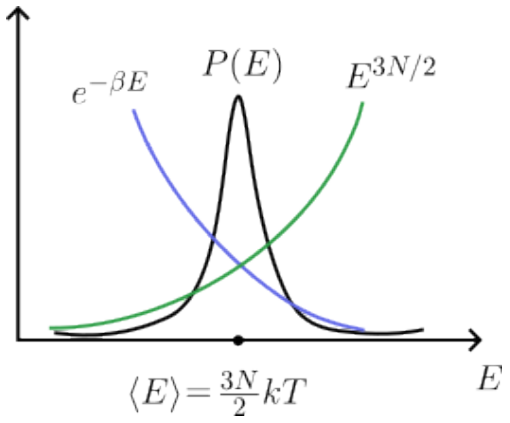
\includegraphics[width=0.35\linewidth]{Immagini/distribuzione P(E).png}
    \caption{grafico della distribuzione di probabilità $P(E)$.}
    \label{fig: distribuzione P(E)}
\end{figure}

\section{Teorema di equipartizione dell'energia}
Si consideri un sistema di $N$ componenti e si supponga che ogni particella sia priva di struttura e sia descrivibile tramite $d$ coppie di variabili coniugate $(q^i,p_i)$ contenute in uno spazio $d$-dimensionale; per cui in totale si hanno $Nd$ coppie ordinate di coordinate $(q^I,p_I)$ con $I = 1,\dots,Nd$. Se si considerano ora le particelle come distinguibili\footnote{In caso contrario tutta la discussione si ripete in modo analogo dopo aver inserito il fattore di indistinguibilità $1/N!$.}, la funzione di partizione è
\begin{equation}
    Z(\beta,V,N) = \int\frac{d^{Nd}q\,d^{Nd}p}{h^{Nd}}e^{-\beta H(q,p)} \equiv \int d\mu\,e^{-\beta H}.
\end{equation}
Ci si concentra ora sull'importante classe di hamiltoniane omogenee di grado secondo nelle $(Nd)$ coordinate di impulso e nelle $Nf_q$ coordinate di posizione non cicliche.
\begin{ex}
    Alcuni esempi di hamiltoniane omogenee di grado secondo sono quella del gas ideale di $N$ componenti in tre dimensioni e quella di $N$ oscillatori armonici unidimensionali disaccoppiati, rispettivamente
    \begin{equation}
        H(q,p) = \sum_{i=1}^N\frac{|\vp_i|^2}{2m},\quad H(q,p) = \sum_{i=1}^N\bigg[\frac{|\vp_{i}|^2}{2m} + \frac{1}{2}m_i w_i^2 (q^i)^2\bigg].
    \end{equation}
\end{ex}
Questa classe di hamiltoniane è importante perchè in tutte le situazioni in cui si devono descrivere piccole fluttuazioni di un sistema intorno ad uno stato di equilibrio, determinato da un minimo del potenziale, si ha un termine cinetico e un termine quadratico nelle coordinate $q$ non cicliche, mentre il termine lineare è assente per la condizione di minimo. Quindi, la classe delle hamiltoniane omogenee di grado due è estremamente rilevante per discutere i sistemi le cui componenti sono libere e/o fluttuano rispetto a posizioni di equilibrio. Sempre per queste hamiltoniane vale la relazione di Eulero
\begin{equation}
\label{eq: relazione di Eulero}
    \bigg(\sum_{I=1}^{Nd}p_I\frac{\p}{\p p_I} + \sum_{J=1}^{Nf_q}q_J\frac{\p}{\p q_J}\bigg)H = 2H,
\end{equation}
il cui valore medio corrisponde a 
\begin{equation}
\label{eq: valore medio relazione di Eulero}
    \vmedio{H(q,p)} \equiv \vmedio{E} = \frac{1}{2}\bigg(\sum_{I=1}^{Nd}\bigvmedio{p_I\frac{\p H}{\p p_I}} + \sum_{J=1}^{Nf_q}\bigvmedio{q^J\frac{\p H}{\p q^J}}\bigg).
\end{equation}
Si consideri il primo termine a secondo membro dell'espressione \eqref{eq: valore medio relazione di Eulero}, in generale si ha
\begin{equation}
    \bigvmedio{p_I\frac{\p H}{\p p_I}} = \frac{1}{Z}\int d\mu\,p_I\frac{\p H}{\p p_I}e^{-\beta H} =  \frac{1}{Z}\int d\mu\, p_I\bigg(-\frac{1}{\beta}\bigg)\frac{\p }{\p p_I}e^{-\beta H},\quad\forall I,
\end{equation}
il quale integrato per parti, osservando che i termini di bordo sono nulli per $p_I\to\pm\infty$ a causa del termine $\exp{(-\beta|\vp_I|^2)/2m}$ in $H$, si ottiene
\begin{equation}
    \bigvmedio{p_I\frac{\p H}{\p p_I}} = \frac{1}{\beta Z}\int d\mu\,\frac{\p p_I}{\p p_I}e^{-\beta H} = \frac{1}{\beta} \equiv kT.
\end{equation}
Quindi, il valore medio rispetto a qualsiasi componente dell'impulso è sempre pari a $kT$. Analogamente, per il secondo termine si ha
\begin{equation}
\label{eq: primo termine valore medio relazione di Eulero}
    \bigvmedio{q^J\frac{\p H}{\p q^J}} = \frac{1}{Z}\int d\mu\,q^J\frac{\p H}{\p q^J}e^{-\beta H} =  \frac{1}{Z}\int d\mu\,q^J\bigg(-\frac{1}{\beta}\bigg)\frac{\p}{\p q^J}e^{-\beta H},\quad\forall J,
\end{equation}
il quale integrato per parti, osservando che i termini di bordo sono nulli in quanto si assume che $H$ contenga il termine di potenziale che cresce con $q^J$ confinando così il sistema, si ottiene nuovamente
\begin{equation}
\label{eq: secondo termine valore medio relazione di Eulero}
    \bigvmedio{q^J\frac{\p H}{\p q^J}} = \frac{1}{\beta Z}\int d\mu\,\frac{\p q^J}{\p q^J}e^{-\beta H} = \frac{1}{\beta} \equiv kT.
\end{equation}
Dunque, sostituendo i risultati ottenuti nella \eqref{eq: primo termine valore medio relazione di Eulero} e \eqref{eq: secondo termine valore medio relazione di Eulero} nella \eqref{eq: valore medio relazione di Eulero}, svolgendo la somma sugli indici $I$ e $J$, si ricava la ``relazione di equipartizione dell'energia'' 
\begin{equation}
\label{eq: relazione di equipartizione dell'energia}
    \vmedio{E} = \frac{1}{2}(Nd + Nf_q)\frac{1}{\beta} = N(d + f_q)\frac{kT}{2}.
\end{equation}
Essenzialmente, la relazione \eqref{eq: relazione di equipartizione dell'energia} afferma che ogni coordinata di tipo $q$ o $p$ che compare nell'hamiltoniana contribuisce all'energia interna con la stessa quantità $kT/2$. 
\begin{obs}
    Dalla \eqref{eq: relazione di equipartizione dell'energia} segue che la capacità termica è indipendente dalla temperatura; infatti
    \begin{equation}
        c_{V,N} = \frac{\p \vmedio{E}}{\p T}\bigg|_{V,N} = N(d + f_q)\frac{k}{2}.
    \end{equation}
    Tuttavia, questo comportamento della capacità termica, inevitabilmente previsto nel contesto classico, è inconsistente con il comportamento reale.
\end{obs}

\section{Teorema del viriale}
Si consideri per semplicità una situazione in cui non sono presenti coordinate cicliche, ossia dove tutte le $\vq^i$ compaiono nell'hamiltoniana, per cui $f_q = d$. Si assuma poi che l'unica dipendenza dagli impulsi sia nel termine cinetico 
\begin{equation}
    K = \sum_{i=1}^{Nd} \frac{|\vp_i|^2}{2m}
\end{equation}
il quale è omogeneo di grado secondo, così che
\begin{equation}
\label{eq: valore medio termine cinetico (teorema viriale)}
    \vmedio{K} = \frac{1}{2} \sum_{i=1}^{Nd} \bigvmedio{p_i \frac{\partial K}{\partial p_i}} = \frac{Nd}{2}kT
\end{equation}
dove nel secondo passaggio si è usata la \eqref{eq: primo termine valore medio relazione di Eulero}. Le equazioni di Hamilton affermano che
\begin{equation}
    \frac{\p H}{\p q_I} = -\dot{p}_I = -F_I, \quad I \equiv (i,a),\,i=1,\cdots,N,\,a = 1,2,3,
\end{equation}
dove $F_I$ è la $a$-esima componente della forza agente sulla $i$-esima particella. Quindi, il ``viriale'' del sistema è definito come
\begin{equation}
    \vps = \nsum_i q^i F_i = \sum_{I=1}^{Nd} q^I F_I,
\end{equation}
il cui valor medio, usando l'equazione di Hamilton per $q^I$, è
\begin{equation}
\label{eq: valore medio viriale (teorema viriale)}
    \vmedio{\vps} = -\nsum_i \bigvmedio{q^i\frac{\partial H}{\partial q^i}} = -NdkT
\end{equation}
avendo usato nell'ultimo passaggio la \eqref{eq: secondo termine valore medio relazione di Eulero}. Confrontando la \eqref{eq: valore medio termine cinetico (teorema viriale)} e la \eqref{eq: valore medio viriale (teorema viriale)} si trova che
\begin{equation}
\label{eq: teorema del viriale}
    \vmedio{\vps} = -2\vmedio{K}.
\end{equation}
L'espressione \eqref{eq: teorema del viriale} è analoga al ``teorema del viriale''\footnote{La prima formulazione del teorema è dovuta a Clausius nel 1870; il nome viriale deriva dal latino ``vis'' significa forza o energia.} in Meccanica classica, il quale afferma che il valor medio temporale del viriale è uguale al doppio del valor medio dell'energia cinetica temporale cambiato di segno, in breve
\begin{equation}    
    \vmedio{\vps}_t = -2\vmedio{K}_t.
\end{equation}

\section{Teorema di Nernst}
L'energia interna termodinamica $E$, corrispondente nell'ensemble canonico a $\vmedio{E}$, è una funzione monotona crescente della temperatura $T$; infatti
\begin{equation}
    c_{V,N} = \frac{\p E}{\p T}\bigg|_{V,N} \ge 0,
\end{equation}
come già era noto a partire dalle condizioni di stabilità termodinamiche e dal legame di $c_{V,N}$ con la varianza $\sigma_E^2$ delle fluttuazioni energetiche \eqref{eq: relazione tra le fluttuazioni di E e cV,N (canonico)}. Quindi, a temperatura $T = 0$, l'energia deve essere la minima possibile e il sistema si deve trovare nello stato fondamentale. Riguardo a quest'ultimo punto si devono distinguere due casi.
\setcounter{caso}{0}
\begin{caso}[stato fondamentale non degenere]
    Se lo stato fondamentale non è degenere, allora ne esiste solamente uno che si indica con $\nu_0$ e la probabilità che il sistema sia in un microstato generico a $T=0$ è semplicemente $P(\nu) = \delta_{\nu,\nu_0}$. In questo caso, l'entropia si annulla dato che il sistema non può cambiare microstato
    \begin{equation}
        \begin{split}
            S = -k\nsum_\nu P(\nu)\log{P(\nu)} = -k\nsum_\nu\delta_{\nu,\nu_0}\log{P(\nu_0)} &= -k\log{P(\nu_0)} \\
            &= -k\log{1} \\
            &= 0.
        \end{split}
    \end{equation}
    Il risultato appena trovato è proprio il contenuto del teorema di Nernst, il quale afferma che l'entropia si annulla allo zero assoluto. Da ciò segue che anche la capacità termica si deve annullare a $T \to 0$, infatti
    \begin{equation}
        c_{V,N} = T\frac{\p S}{\p T} \to 0
    \end{equation}
    dato che $\p S/\p T$ non può divergere per $T \to 0$ dato che $S \to 0$. Il fatto che $c_{V,N} \to 0$ per $T \to 0$ è in netto contrasto con il risultato proveniente dal teorema di equipartizione; tuttavia, l'errore non è qui, ma nell'equipartizione. Infatti, in quel contesto si era ipotizzato che il sistema fosse trattabile classicamente, ma trascurando il fatto che per temperature basse non può essere tralasciata la descrizione quantistica del sistema. Pertanto, l'equipartizione vale solo nel limite classico.
\end{caso}
\begin{caso}[stato fondamentale degenere]
    Se lo stato fondamentale è degenere, allora esistono $m$ stati distinti $\nu_{0,i}$ di energia minima. Avendo tutti la medesima energia, i microstati sono tutti equiprobabili con probabilità $1/m$, per cui
    \begin{equation}
        P(\nu) = 
        \begin{cases}
            1/m,\quad \forall i =1,\dots,m \\
            0,\quad \nu \neq \nu_{0,i}
        \end{cases}.
    \end{equation}
    In questo caso, l'entropia non si annulla allo zero assoluto, ma compare un'entropia ``residua''
    \begin{equation}
        S = -k\nsum_{i = 1}^mP(\nu_{0,i})\log{P(\nu_{0,i})} = -\frac{k}{m}\nsum_{i = 1}^m\log{\frac{1}{m}} = k\log{m}.
    \end{equation}
    Normalmente, il numero di microstati degeneri $m$ non è proporzionale ad $N$ e l'entropia residua è presente ma è molto piccola nel limite termodinamico.
\end{caso}

\section{Solido di Einstein nell'ensemble canonico}
Come già visto nell'ensemble microcanonico, il solido di Einstein è un modello che consiste in $3N$ oscillatori armonici quantistici di frequenza $\omega$ disaccoppiati. Gli $N$ componenti sono non interagenti e indistinguibili, per cui la funzione di partizione del sistema si fattorizza\footnote{Non c'è bisogno di introdurre il fattore di Gibbs dato che gli elementi sono indistinguibili, come prescrive la Meccanica quantistica.} in $Z = [Z_{(1)}]^{3N}$, dove $Z_{(1)}$ è la funzione di partizione del singolo oscillatore armonico quantistico di frequenza $\omega$. Si indica con $\{\ket{n}\}$ a base degli autostati dell'energia per l'oscillatore armonico e si rappresenta la matrice densità in tale base
\begin{equation}
    \rho_{mn} = \frac{e^{-\beta E_n}} {Z_{(1)}}\delta_{mn},\quad Z_{(1)} = \Tr{\hatrho} = \nsum_n e^{-\beta E_n}.
\end{equation}
Dato che gli autostati dell'energia non sono degeneri, l'energia associata vale
\begin{equation}
    E_n = \bigg(n + \frac{1}{2}\bigg)\hbar\omega.
\end{equation}
Quindi, si ha che la funzione di partizione parziale, usando la nozione di serie geometrica, è
\begin{equation}
\label{eq: funzione di partizione singola particella solido di Einstein (canonico)}
    \begin{split}
        Z_{(1)} = \nsum_n e^{-\beta(n + 1/2)\hbar\omega} &= e^{-\beta\hbar\omega/2}\nsum_n(e^{-\beta\hbar\omega})^n \\
        &= \frac{e^{-\beta\hbar\omega}}{1 - e^{-\beta\hbar\omega}} \\
        &= \bigg(2\sinh{\frac{\beta\hbar\omega}{2}}\bigg)^{-1},
    \end{split}
\end{equation}
da cui segue immediatamente che
\begin{equation}
    Z = \bigg(2\sinh{\frac{\beta\hbar\omega}{2}}\bigg)^{-3N}.
\end{equation}
Ora, ottenuta la funzione di partizione del sistema, è possibile ricavare tutte le grandezze termodinamiche. Prima di tutto, l'energia libera è data da
\begin{equation}
    F = -\frac{\log{Z}}{\beta} = \frac{3N}{\beta}\log{\bigg(2\sinh{\frac{\beta\hbar\omega}{2}}\bigg)};
\end{equation}
invece, l'energia termodinamica è
\begin{equation}
    E \equiv \vmedio{E} = -\frac{\p\log{Z}}{\p\beta} = \frac{3N\hbar\omega}{2}\coth{\frac{\beta\hbar\omega}{2}} = 3N\hbar\omega\bigg(\frac{1}{e^{\beta\hbar\omega} - 1} + \frac{1}{2}\bigg),
\end{equation}
in accordo con quanto trovato nell'ensemble microcanonico con la \eqref{eq: energia solido di Einstein (microcanonico)}. Chiaramente, nel regime di alta temperatura si ritrova il risultato classico $\vmedio{E} = 3NkT$ per $kT \gg \hbar\omega$, ricavabile dal teorema di equipartizione per $3N$ oscillatori con $d = 1$ e $f_q = 1$.

\subsection{Rotazione di Wick}
Esiste una profonda relazione tra la trattazione statistica di un sistema quantistico e la ``rotazione di Wick'', una particolare trasformazione agente sulla coordinata temporale. Si consideri quindi un sistema quantistico con un solo grado di libertà $q$, che si può pensare come singola componente di un sistema non interagente. 
\begin{obs}
    Per sistemi interagenti si dovrebbero considerare innumerevoli gradi di libertà; formalmente la generalizzazione non è un problema.
\end{obs}
Siano $\ket{q}$ gli autostati dell'operatore posizione e $\ket{q(t)}$ i corrispondenti stati nella descrizione di Schr\"odinger che evolvono nel tempo tramite
\begin{equation}
    \ket{q(t)} = e^{i\hatH t/\hbar}\ket{q}.
\end{equation}
Si introduce ora il ``nucleo'', o ``kernel'', $K(q_f,q_i;t_f,t_i)$ come
\begin{equation}
\label{eq: definizione kernel}
    K(q_f,q_i;t_f,t_i) = \mybraket{q_f(t_f)}{q_i(t_i)},
\end{equation}
il quale descrive la probabilità che il sistema si trovi nella posizione $q_f$ al tempo $t_f$ a partire dalla posizione $q_i$ al tempo $t_i$. Si supponga ora di effettuare una rotazione di Wick rimpiazzando il tempo $t$ con il ``tempo euclideo'' $\tau \in \R$ secondo la trasformazione $t \to -i\tau$. In questo modo, il kernel \eqref{eq: definizione kernel} diventa il kernel euclideo
\begin{equation}
    K_E(q_f,q_i;\Delta\tau = \tau_f - \tau_i) = \mybrakett{q_f}{e^{-\Delta\tau\hatH/\hbar}}{q_i},
\end{equation}
dove il fattore di evoluzione temporale diventa una fattore di Boltzmann ponendo
\begin{equation}
    \frac{\Delta\tau}{\hbar} = \frac{1}{kT} \equiv \beta,
\end{equation}
arrivando così all'espressione
\begin{equation}
\label{eq: kernel euclideo}
     K_E(q_f,q_i;\Delta\tau = \hbar\beta) = \mybrakett{q_f}{e^{-\beta\hatH}}{q_i}.
\end{equation}
Quindi, il kernel è essenzialmente la matrice densità nella base della posizione con il tempo $\Delta\tau$. Se si definisce la funzione di partizione come la traccia del kernel \eqref{eq: kernel euclideo}, ossia ponendo $q_f = q_i \equiv q$, allora
\begin{equation}
\label{eq: funzione di partizione come traccia del kernel euclideo (canonico)}
    Z_E = \int dq\,K_E(q,q;\Delta\tau) = \int dq\,\mybrakett{q}{e^{-\beta\hatH}}{q} = \Tr{e^{-\beta\hatH}}
\end{equation}
ed è evidente come questa corrisponda alla funzione di partizione canonica, con la traccia presa nella base $\{\ket{q}\}$ degli autostati della posizione. Dalle equazioni \eqref{eq: kernel euclideo} e \eqref{eq: funzione di partizione come traccia del kernel euclideo (canonico)} segue che la matrice densità in tale base è
\begin{equation}
\label{eq: matrice densità in termini del kernel (canonico)}
    \rho_{q_f,q_i} = \frac{1}{Z}K_E(q_f,q_i;\Delta\tau).
\end{equation}
Il kernel può essere espresso in vari modi, uno di questi è tramite l'integrale funzionale
\begin{equation}
\label{eq: kernel come integrale funzionale}
    K(q_f,q_i;t_f,t_i) = \int_{q(t_i)}^{q(t_f)} Dq\,e^{iS[q(t)]/\hbar}.
\end{equation}
L'idea di usare un integrale di cammino si fonda sulla possibilità di in Meccanica quantistica di passare dalla posizione iniziale a quella finale facendo un integrale sulle traiettorie, opportunamente pesate da un esponenziale dipendente dal funzionale di azione $S[q(t)]$. Tra tutte le possibili traiettorie, quella corrispondente alla traiettoria classica è quella con il peso maggiore, tutte le altre avranno un peso minore di questa. Rispetto ad una rotazione di Wick, si può definire l'azione euclidea $S_E[q(t)]$ come
\begin{equation}
    iS[q(t)] \to -S_E[q(\tau)],\quad t \to -i\tau.
\end{equation}
In questo modo, la funzione di partizione \eqref{eq: funzione di partizione come traccia del kernel euclideo (canonico)} diventa anch'essa euclidea
\begin{equation}
\label{eq: funzione di partizione come integrale funzionale euclideo (canonico)}
    Z_E = \int_{PBC}Dq\,e^{-S_E[q(\tau)]/\hbar},
\end{equation}
dove le funzioni $q(\tau)$ obbediscono alle ``periodic boundary conditions'' (PBC) definite da
\begin{equation}
\label{eq: PBC}
    q(\tau_i) = q(\tau_f) = q(\tau_i + \Delta\tau) = q(\tau_i + \hbar\beta).
\end{equation}
Si nota che proprio in queste condizioni al bordo entra in gioco la temperatura del sistema. La funzione di partizione dell'integrale canonico a temperatura $T$ può quindi essere calcolata tramite l'integrale funzionale euclideo \eqref{eq: funzione di partizione come integrale funzionale euclideo (canonico)} imponendo le condizioni al bordo periodiche \eqref{eq: PBC}. Geometricamente, la funzione di partizione così definita corrisponde alla ``compattificazione'' del tempo euclideo su un cerchio di lunghezza $\hbar\beta$, come rappresentato in figura \ref{fig: compattificazione tempo euclideo}.
\begin{figure}[h]
    \centering
    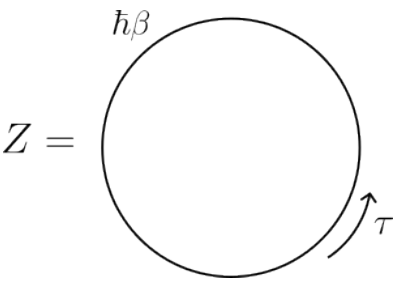
\includegraphics[width=0.35\linewidth]{Immagini/compattificazione tempo euclideo.png}
    \caption{compattificazione del tempo euclideo su un cerchio $S_1$.}
    \label{fig: compattificazione tempo euclideo}
\end{figure}

Analogamente alla \eqref{eq: funzione di partizione come integrale funzionale euclideo (canonico)}, anche il kernel euclideo può essere espresso in funzione di $S_E$ tramite
\begin{equation}
\label{eq: kernel euclideo come integrale funzionale}
    K_E(q_f,q_i;\tau_f,\tau_i) = \int_{q(\tau_i)}^{q(\tau_f)} Dq\,e^{-S_E[q(\tau)]/\hbar}.
\end{equation}
Tramite la \eqref{eq: matrice densità in termini del kernel (canonico)}, la conoscenza del kernel euclideo e della funzione di partizione euclidea fornisce la matrice densità nella base degli autostati della posizione. Tuttavia, la matrice può anche essere calcolata a partire dalla base dell'energia; infatti, se $\{\ket{n}\}$ sono gli stati stazionari, sfruttando la relazione di completezza nella \eqref{eq: kernel euclideo}, si ha
\begin{equation}
\label{eq: kernel in termini delle funzioni d'onda stati stazionari (canonico)}
    \begin{split}
        K_E(q_f,q_i;\Delta\tau) &= \nsum_n\mybraket{q_f}{n}\mybrakett{n}{e^{-\beta\hatH}}{q_i} \\
        &= \nsum_n\mybraket{q_f}{n}\mybraket{n}{q_i}e^{-\beta E_n} \\
        &= \nsum_n u^*_n(q_f)u_n(q_i)e^{-\beta E_n},
    \end{split}
\end{equation}
dove le $u_n(q)$ sono le funzioni d'onda degli stati stazionari.
\begin{ex}
    Per un oscillatore armonico quantistico di frequenza $\omega$, l'azione è
    \begin{equation}
        iS[q(t)] = i\int_{t_i}^{t_f} dt\,\bigg(\frac{m}{2}\dot{q}^2 - \frac{1}{2}m\omega^2q^2\bigg),
    \end{equation}
    la quale sotto rotazione di Wick diventa l'azione euclidea
    \begin{equation}
        S_E[q(\tau)] = \int_{\tau_i}^{\tau_f}d\tau\,\bigg[\frac{m}{2}\bigg(\frac{dq}{d\tau}\bigg)^2 + \frac{1}{2}m\omega^2q^2\bigg].
    \end{equation}
    Di conseguenza, il kernel euclideo è
    \begin{equation}
        K_E(q_f,q_i;\Delta\tau) = \int_{q(\tau_i)}^{q(\tau_f)}Dq(\tau)\,\exp{\bigg\{-\int_{\tau_i}^{\tau_f}d\tau\,\bigg[\frac{m}{2}\bigg(\frac{dq}{d\tau}\bigg)^2 + \frac{1}{2}m\omega^2q^2\bigg]\bigg\}}.
    \end{equation}
    Questo può essere calcolato esplicitamente dividendo $q(\tau)$ in una traiettoria classica $q(\tau)_c$ che soddisfa le equazioni del moto e in una fluttuazione quantistica $x(\tau)$, per cui $q(\tau) := q(\tau)_c + x(\tau)$. Il passo successivo è il calcolo dell'integrale funzionale sulle fluttuazioni, omettendo questo passaggio per semplicità, il risultato finale è
    \begin{equation}
        \begin{split}
            K_E(q_f,q_i;\Delta\tau) &= \sqrt{\frac{m\omega}{2\pi\hbar\sinh{\beta\hbar\omega}}} \\
            &\times\exp{\bigg\{-\frac{m\omega}{2\hbar\sinh{\beta\hbar\omega}}[(q_i^2 + q_f^2)\cosh{(\beta\hbar\omega) - 2q_iq_f}]\bigg\}}.
        \end{split}
    \end{equation}
    A questo punto, la funzione di partizione è direttamente ricavabile dalla \eqref{eq: funzione di partizione come integrale funzionale euclideo (canonico)}; l'espressione da risolvere è un integrale gaussiano, il cui risultato è
    \begin{equation}
        Z = \bigg(2\sinh{\frac{\beta\hbar\omega}{2}}\bigg)^{-1},
    \end{equation}
    in perfetto accordo con quanto trovato nella \eqref{eq: funzione di partizione singola particella solido di Einstein (canonico)}. La relazione \eqref{eq: matrice densità in termini del kernel (canonico)} permette di determinare la matrice densità nella base delle posizioni; in particolare, i termini diagonali di $\rho_{qq}$ che rappresentano la probabilità che l'oscillatore ``termalizzato'' si trovi nella posizione $q$ sono dati da
    \begin{equation}
        \begin{split}
            \rho_{qq} &= 2\sinh{\frac{\beta\hbar\omega}{2}}\sqrt{\frac{m\omega}{2\pi\hbar\sinh{\beta\hbar\omega}}}\exp{\bigg\{-\frac{2m\omega\sinh{(\beta\hbar\omega/2)}}{\hbar\sinh{\beta\hbar\omega}}q^2\bigg\}} \\
            &= \sqrt{\frac{m\omega}{\pi\hbar}\tanh{\frac{\beta\hbar\omega}{2}}}\exp{\bigg\{-\frac{m\omega}{\hbar}\tanh{\bigg(\frac{\beta\hbar\omega}{2}\bigg)}q^2\bigg\}},
        \end{split}
    \end{equation}
    dove si è usata la relazione trigonometrica
    \begin{equation}
        \sinh{\beta\hbar\omega} = 2\sin{\bigg(\frac{\beta\hbar\omega}{2}\bigg)}\cos{\bigg(\frac{\beta\hbar\omega}{2}\bigg)}.
    \end{equation}
\end{ex}

\subsection{Condizioni al bordo periodiche}
L'obiettivo adesso è dimostrare che nel limite termodinamico la forma delle condizioni al contorno è irrilevante e, di conseguenza, è possibile scegliere le condizioni al contorno più convenienti a seconda del sistema in esame. Per semplicità, si considera un gas di particelle quantistiche non interagenti, la cui funzione di partizione si fattorizza secondo \eqref{eq: funzione di partizione sistemi non interagenti (canonico)} in termini di quella associata alla singola particella $Z_{(1)}$. Ancora per motivi di semplicità, si suppone che il gas sia confinato in un cubo di lato $L$; comunque, in ogni caso è possibile dimostrare che anche la forma del volume contente il sistema è irrilevante. Essendo la particella libera, il problema tridimensionale si decompone in tre copie del problema di una particella confinata in una buca infinita di potenziale unidimensionale. Le autofunzioni dell'hamiltoniana $\hatH = -(-\hbar^2/2m)\nabla^2$ sono
\begin{equation}
\label{eq: funzione d'onda stati stazionari buca di potenziale (canonico)}
    u_n(x) = \sqrt{\frac{2}{L}}\sin{k_n x},\quad k_n \equiv \frac{\pi n}{L},
\end{equation}
le quali soddisfano le condizioni di annullamento $u_n(0) = u_n(L) = 0$ e sono tali che 
\begin{equation}
\label{eq: energie stati stazionari buca di potenziale (canonico)}
    \hatH u_n = E_nu_n,\quad E_n = \frac{(\hbar\pi n)^2}{2mL} \equiv n^2 E_1,
\end{equation}
oltre ad essere normalizzate tramite
\begin{equation}
    \int_0^L dx\,|u_n(x)|^2 = 1.
\end{equation}
I livelli di energia non sono degeneri, per cui la funzione di partizione vale
\begin{equation}
\label{eq: funzione di partizione particella buca di potenziale (canonico)}
    Z_x = \nsum_n e^{-\beta E_n} = \nsum_n e^{-\beta n^2E_1}.
\end{equation}
Si nota adesso che il termine $\beta E_1$ può essere espresso in termini della lunghezza d'onda termica $\lambda_T$ introdotta nella \eqref{eq: funzione di partizione singola particella (canonico)}, infatti
\begin{equation}
    \beta E_1 = \frac{\beta\hbar^2\pi^2}{2mL^2} = \frac{\pi}{4}\frac{\beta h^2}{2\pi m}\frac{1}{L^2} = \frac{\pi}{4}\bigg(\frac{\lambda_T}{L}\bigg)^2.    
\end{equation}
L'espressione \eqref{eq: funzione di partizione particella buca di potenziale (canonico)} è esatta, tuttavia si può considerare il suo sviluppo in due casi diversi.
\setcounter{caso}{0}
\begin{caso}[bassa temperatura]
    Nel limite di bassa temperatura, l'energia termica è molto minore dell'energia dello stato fondamentale del sistema, per cui
    \begin{equation}
        kT \ll E_1 \quad\Longleftrightarrow\quad \lambda_T \gg L.
    \end{equation}
    In questo regime la soppressione esponenziale nella \eqref{eq: funzione di partizione particella buca di potenziale (canonico)} è estremamente efficace e quindi
    \begin{equation}
    \label{eq: sviluppo bassa T funzione di partizione particella buca di potenziale (canonico)}
        Z_x = e^{-\beta E_1} + e^{-4\beta E_1} + \cdots \simeq e^{-(\pi/4)(\lambda_T/L)^2},
    \end{equation}
    per cui la funzione di partizione riceve quasi esclusivamente il contributo dello stato fondamentale. Questo risultato non è di particolare interesse, se non per il fatto che classicamente non è prevista una tale situazione.
\end{caso}
\begin{caso}[alta temperatura]
    Nel limite di alta temperatura, ci si aspetta di ritrovare il risultato derivato dalla trattazione classica; in questo caso
    \begin{equation}
        kT \gg E_1 \quad\Longleftrightarrow\quad \lambda_T \ll L.
    \end{equation}
    Questa volta, la soppressione esponenziale nella \eqref{eq: funzione di partizione particella buca di potenziale (canonico)} non è così efficace in quanto adesso tutti gli elementi della serie contribuiscono a $Z_x$; pertanto, è necessario risommare la serie tramite la ``risommazione di Poisson'', di seguito esposta.
    \begin{teo}[Risommazione di Poisson]
        Data una funzione $f(x)$ e sia $\tilde{f}(p)$ la sua antitrasformata di Fourier data da
        \begin{equation}
            \tilde{f}(p) = \int dx\,e^{-ipx}f(x),
        \end{equation}
        allora vale la formula
        \begin{equation}
        \label{eq: risommazione di Poisson}
            \sum_{n\in\Z}f(n) = \sum_{r\in\Z}\tilde{f}(2\pi r).
        \end{equation}
    \end{teo}
    Quindi, si riscrive la funzione di partizione \eqref{eq: funzione di partizione particella buca di potenziale (canonico)} come\footnote{Si vuole la sommatoria su tutti gli interi, ma in $Z$ si ha solo quella sugli interi positivi. Però, essendo pari, si può riscrivere $Z$ come la somma $(1/2)\nsum_n$. Tuttavia, facendo la somma su tutti gli $n$ si considera anche il caso non interessante $n = 0$, per cui lo si sottrae considerando che $e^0 = 1$.}
    \begin{equation}
        Z_x = \frac{1}{2}\bigg(\sum_{n\in\Z}e^{-(\pi/4)(\lambda_T/L)^2n^2} - 1\bigg) \equiv \frac{1}{2}\bigg(\sum_{n\in\Z}f(n) - 1\bigg),
    \end{equation}
    applicando la formula di Poisson \eqref{eq: risommazione di Poisson} con 
    \begin{equation}
        \tilde{f}(r) = \int dn\,e^{-irn}e^{-(\pi/4)(\lambda_T/L)^2n^2} = \frac{2L}{\lambda_T}e^{-r^2L/\lambda_T\pi},
    \end{equation}
    ottenendo così 
    \begin{equation}
        Z_x = \frac{1}{2}\bigg(\frac{2L}{\lambda_T}\sum_{r\in\Z}e^{-4\pi r^2(L/\lambda_T)^2} - 1\bigg).
    \end{equation}
    Quindi, nel limite di alta temperatura si ha che $L/\lambda_T \gg 1$ e quindi ora la soppressione esponenziale è efficace
    \begin{equation}
    \label{eq: sviluppo alta T funzione di partizione particella buca di potenziale  (canonico)}
        Z_x \simeq \frac{1}{2}\bigg[\frac{2L}{\lambda_T}(1 + \cdots) - 1\bigg] \simeq \frac{L}{\lambda_T}\bigg(1 - \frac{\lambda_T}{2L} + \cdots \bigg) \simeq \frac{L}{\lambda_T}.
    \end{equation}
    Questo risultato corrisponde al caso classico, infatti dato che $Z_x  = Z_y = Z_z$, in tre dimensioni si ottiene proprio \eqref{eq: funzione di partizione singola particella (canonico)}.
\end{caso}
\begin{obs}
    Esiste un modo più semplice per ottenere lo stesso risultato per il termine dominante\footnote{La risommazione di Poisson permette di ottenere anche tutti i termini sottodominanti, ma in questo caso non sono di particolare interesse.}. Quest'ultimo si ottiene se si sostituisce la sommatoria su $n$ nella \eqref{eq: funzione di partizione particella buca di potenziale (canonico)} con un integrale, cioè facendone il limite al continuo. Infatti, nel limite di alta temperatura i livelli quantistici sono quasi continui. Per fare, si usa la formula di Eulero-MacLaurin\footnote{La formula di Eulero-MacLaurin è 
    \begin{equation}
        \sum_{n = p+1}^qf(n) = \int_p^q dn\,f(n) + \sum_{k=1}^r\frac{B_k}{k!}[f^{(k-1)}(q) - f^{(k-q)}(p)] + R_r,
    \end{equation}
    dove i $B_k$ sono i ``numeri di Bernoulli''.}, così si ha
    \begin{equation}
        \nsum_n \longrightarrow \int dn = \frac{L}{\pi} \int dk,
    \end{equation}
    dove si è introdotto il numero d'onda continuo $k$ per rimpiazzare i valori discreti $k_n$. Quindi, dalla \eqref{eq: funzione di partizione particella buca di potenziale (canonico)} si ottiene un integrale gaussiano e il medesimo risultato
    \begin{equation}
        \begin{split}
            Z_x \simeq \frac{1}{2} \bigg( \frac{L}{\pi} \int_\R dk\, e^{-\lambda_T^2k^2/4\pi^2} - 1 \bigg) &= \frac{1}{2} \bigg( \frac{L}{\pi} \sqrt{\frac{4\pi^2}{\lambda_T^2}} - 1 \bigg)  \\
            &= \frac{1}{2} \bigg( \frac{2L}{\lambda_T} - 1 \bigg) \\
            &\simeq \frac{L}{\lambda_T}.
        \end{split}
    \end{equation}
\end{obs}
Ora si supponga di imporre delle condizioni al bordo periodiche generiche, anche se non sarebbero adatte al problema della particella confinata in una buca infinita di potenziale $u(x) = u(x + L)$; con tali condizioni, gli stati stazionari hanno come funzione d'onda
\begin{equation}
    \tilde{u}_n(x) = \frac{1}{\sqrt{L}}e^{i\tilde{k_n}x},\quad \tilde{k}_n = \frac{2\pi n}{L}
\end{equation}
ed energie
\begin{equation}
    \tilde{E}_n = \frac{\hbar^2\tilde{k}_n^2}{2m} = n^2\tilde{E}_1.
\end{equation}
Dal confronto con la \eqref{eq: energie stati stazionari buca di potenziale (canonico)} segue immediatamente che
\begin{equation}
    \tilde{E}_n = 4E_n.
\end{equation}
La funzione di partizione è
\begin{equation}
\label{eq: funzione di partizione particella buca di potenziale tilde (canonico)}
    \tilde{Z}_x  =\sum_{n\in\Z}e^{-\beta \tilde{E}_n} = \sum_{n\in\Z}e^{-\beta \tilde{E}_1n^2},\quad \beta\tilde{E}_1 = -\pi\bigg(\frac{\lambda_T}{L}\bigg)^2.
\end{equation}
La sommatoria che appare nell'espressione esatta \eqref{eq: funzione di partizione particella buca di potenziale tilde (canonico)} corrisponde ad una delle ``costanti $\theta$ di Jacobi'' molto importanti in Matematica; in particolare, corrisponde alla $\theta_3$ definita come
\begin{equation}
\label{eq: definizione funzione theta3 di Jacobi}
    \theta_3(v|\tau) = \sum_{n\in\Z}e^{i\pi\tau n^2 + 2\pi ivn} \equiv \theta_3(\tau)\sum_{n\in\Z}e^{2\pi ivn}.
\end{equation}
Quindi, si può scrivere la \eqref{eq: funzione di partizione particella buca di potenziale tilde (canonico)} come 
\begin{equation}
    \tilde{Z}_x = \theta_3\bigg(\frac{i\beta\tilde{E}_1}{\pi}\bigg) = \theta_3\bigg[i\bigg(\frac{\lambda_T}{L}\bigg)^2\bigg],
\end{equation}
su cui è possibile applicare la risommazione di Poisson. Sulle costanti $\theta$ di Jacobi tale risommazione equivale alla proprietà di ``dualità'', che consiste in
\begin{equation}
    \theta_3(\tau) = (-i\tau')^{1/2}\theta_3(\tau'),\quad \tau \to \tau' = -\tau^{-1}.
\end{equation}
Essenzialmente, la $\theta_3$ valutata su un certo argomento è collegata in modo semplice alla $\theta_3$ valutata nell'inverso di tale argomento; in questo caso
\begin{equation}
    \tau = i\bigg(\frac{\lambda_T}{L}\bigg)^2 \to \tau ' = -\bigg(i\frac{\lambda_T}{L}\bigg)^{-2}.
\end{equation}
Detto ciò, come prima si devono distinguere i due limiti un funzione della temperatura.
\setcounter{caso}{0}
\begin{caso}[bassa temperatura]
    Nel limite di bassa temperatura, l'espansione di $\tilde{Z}_x$ è molto diversa da quella di $Z_x$ riportata in \eqref{eq: sviluppo bassa T funzione di partizione particella buca di potenziale (canonico)}, infatti ora
    \begin{equation}
        \tilde{Z}_x = 1 + 2e^{-\beta\tilde{E}_1} + \cdots = 1 + 2e^{-\pi\lambda_T^2/L^2} + \cdots,
    \end{equation}
    dove il termine esponenziale non è dominante. Quindi, in questo limite la particella si trova quasi sicuramente nello stato fondamentale, e questi con le due diverse condizioni al contorno sono diversi.
\end{caso}
\begin{caso}[alta temperatura]
    Nel limite di alta temperatura si può effettuare la risommazione di Poisson ottenendo
    \begin{equation}
        \begin{split}
            \tilde{Z}_x = \sum_{n\in\Z} e^{-\pi(\lambda_T/L)^2n^2} &= \frac{L}{\lambda_T}\sum_{r\in\Z}e^{-\pi(L/\lambda_T)^2r^2} \\
            &= \frac{L}{\lambda_T}\bigg[1 + 2e^{-\pi(L/\lambda_T)^2} + \cdots\bigg] \\
            &\simeq Z_x.
        \end{split}
    \end{equation}
    Dunque, in questo limite le funzioni di partizione calcolate con diverse condizioni al contorno coincidono: per un sistema con molte componenti di questo tipo la termodinamica da esse derivata è la medesima. In realtà non è proprio così, in quanto potrebbero esistere alcune osservabili localizzate vicino al bordo più sensibili al fatto di aver cambiato le condizioni al contorno. Per questo si dice che le condizioni al contorno sono ``quasi irrilevanti''.
\end{caso}

\subsubsection{Generalizzazione unidimensionale}
Il fatto che le condizioni siano quasi irrilevanti può essere generalizzato. Per modellizzare il comportamento termodinamico descritto dall'energia libera $F(T,V,N,\dots)$ si può fissare il volume $V$ del sistema confinandolo in una regione qualsiasi forma sia più conveniente, assegnando condizioni al contorno altrettanto vantaggiose per l'analisi. Tuttavia, questo non significa che tutte le osservabili siano indipendenti dalle condizioni al contorno; infatti, una generica osservabile $O$ ha un valore medio statistico dato da
\begin{equation}
    \vmedio{\hatO} = \Tr{\hatO\hatrho},\quad\hatrho = \frac{e^{-\beta\hatH}}{Z}.
\end{equation}
L'operatore densità, ad esempio rappresentato tramite la matrice associata nella base degli autostati della posizione $\rho(x',x) = \mybrakett{x'}{\hatrho}{x}$, in generale dipende dalle condizioni al contorno, influenzando di conseguenza il calcolo delle osservabili localizzate nei pressi del bordo del sistema. 

Si riconsideri il caso della particella quantistica confinata in una buca infinita di potenziale, dalla \eqref{eq: kernel in termini delle funzioni d'onda stati stazionari (canonico)} si ha
\begin{equation}
    \rho(x',x) = \mybrakett{x'}{\hatrho}{x} = \frac{1}{Z_x}\nsum_nu_n^*(x')u_n(x)e^{-\beta E_n}
\end{equation}
che, con la \eqref{eq: funzione d'onda stati stazionari buca di potenziale (canonico)} e la \eqref{eq: energie stati stazionari buca di potenziale (canonico)}, diventa
\begin{equation}
\label{eq: matrice densità buca di potenziale (canonico)}
    \rho(x',x) = \frac{2}{Z_xL}\nsum_n\sin{(kx')}\sin{(kx)}e^{-\lambda_T^2k^2/4\pi},\quad k = \frac{n\pi}{L}.
\end{equation}
Nel limite di alta temperatura, si può passare al continuo tramite la formula di Eulero-MacLaurin, ottenendo
\begin{equation}
    \rho(x',x) = \frac{2}{Z_x\cancel{L}}\frac{\cancel{L}}{\pi}\int_0^\infty dk\,\sin{(kx')}\sin{(kx)}e^{-\lambda_T^2k^2/4\pi}.
\end{equation}
Il risultato finale dell'integrale, di cui si omettono i passaggi di risoluzione per semplicità, è
\begin{equation}
    \rho(x',x) = \frac{1}{Z_x\lambda_T}\bigg[e^{-\pi(x' - x)^2/\lambda_T^2} - e^{-\pi(x' + x)^2/\lambda_T^2} \bigg].
\end{equation}
In particolare, si osserva che
\begin{equation}
    \rho(x',x) = 0\quad\Longleftrightarrow\quad
    \begin{cases}
        x' = 0 \\
        x = 0
    \end{cases}\quad
    \vee\quad
    \begin{cases}
        x' \simeq L \to \infty \\
        x \simeq L \to \infty
    \end{cases}.
\end{equation}
Questo è consistente con il fatto che si sta descrivendo il sistema con condizioni di annullamento ai bordi, per le quali si deve avere ampiezza di transizione nulla quando ci si trova sul bordo. Invece, i termini diagonali di $\rho(x',x)$ rappresentano la probabilità di trovare la particella termalizzata nella posizione $x = x'$
\begin{equation}
    \rho(x,x) = \frac{1}{Z_x\lambda_T}\bigg(1 - e^{-4\pi x^2/\lambda_T^2}\bigg).
\end{equation}
Dall'espressione di $\rho(x,x)$ si deduce che la distribuzione della probabilità per una particella in scatola è sostanzialmente piatta, eccetto in una regione di dimensione $\lambda_T$ vicino al bordo. Tenendo conto che nel limite di alta temperatura $Z_x\lambda_T \simeq L$ e limitandosi a valori di $x$ ed $x'$ non vicini al bordo, si ha che
\begin{equation}
\label{eq: matrice densità buca di potenziale alta T (canonico)}
    \rho(x',x) \simeq \frac{1}{L}e^{-\pi(x' - x)^2/\lambda_T^2}.
\end{equation}

Si passa adesso determinare la matrice densità che si ottiene imponendo delle condizioni al contorno periodiche. In tal caso, l'analgo della \eqref{eq: matrice densità buca di potenziale (canonico)} usando le \eqref{eq: funzione d'onda stati stazionari buca di potenziale (canonico)} e \eqref{eq: energie stati stazionari buca di potenziale (canonico)}, è
\begin{equation}
    \tilde{\rho}(x',x) = \frac{1}{\tilde{Z}_x}\nsum_n\tilde{u}_n^*(x')\tilde{u}_n(x)e^{-\beta\tilde{E}_n} = \frac{1}{\tilde{Z}_xL}\nsum_ne^{-ik_n(x'-x)}e^{-\pi\lambda_T^2/L^2n^2}.
\end{equation}
Sostituendo la somma discreta con un integrale tramite la formula di Eulero-MacLaurin, nel limite di alta temperatura, si ha
\begin{equation}
\label{eq: matrice densità buca di potenziale alta T tilde (canonico)}
    \begin{split}
        \tilde{\rho}(x',x) &= \frac{1}{\tilde{Z}_x\cancel{L}}\frac{\cancel{L}}{2\pi}\int_\R dk\, e^{-ik(x'-x) - \lambda_T^2k^2/4\pi} \\
        &= \frac{1}{\cancel{2\pi}\tilde{Z}_x}\frac{\cancel{2\pi}}{\lambda_T}e^{-\pi(x'-x)^2/\lambda_T} \\
        &\simeq \frac{1}{L}e^{-\pi(x'-x)^2/\lambda_T^2},
    \end{split}
\end{equation}
la quale coincide esattamente con la $\rho(x',x)$ trovata con le condizioni di annullamento al bordo nella \eqref{eq: matrice densità buca di potenziale alta T (canonico)}, per tutte le $x'$ ed $x$ che non si trovano nei pressi del bordo. Dunque, si nota che in precedenza la matrice densità aveva dei termini che non erano trascurabili nei pressi del bordo, adesso invece questo non accade essendo la $\rho$ nella \eqref{eq: matrice densità buca di potenziale alta T tilde (canonico)} periodica e quindi tutti i punti sono uguali. Pertanto, le differenze determinate dalle condizioni al contorno sono minime e sono solo locali. Tendenzialmente d'ora in poi ci si concentra sulle proprietà termodinamiche ``di bulk'', ossia  non legate ad osservabili localizzate presso il bordo, e si scelgono usualmente condizioni di periodicità
che semplificano i calcoli.

\subsubsection{Generalizzazione tridimensionale}
Si generalizza ora al caso tridimensionale. Sempre nel caso in cui la particella sia confinata in un cubo di di volume $V = L^3$, le autofunzioni di energia sono il prodotto di quelle trovate per ciascuna direzione $x, y, z$. Nel caso periodico si ha
\begin{equation}
    \tilde{u}_{\vn}(\vx) = \frac{1}{\sqrt{V}} \tilde{u}_{n_x}(x)\tilde{u}_{n_y}(y)\tilde{u}_{n_z}(z) = \frac{1}{\sqrt{V}} e^{i\vk(\vn)\cdot \vx},\quad k(\vn) = \frac{2\pi}{L}\vn
\end{equation}
dove $\vn = (n_x, n_y, n_z) \in \Z^3$. L'energia è semplicemente la somma di quelle relative alle tre direzioni
\begin{equation}
    \begin{split}
        E_{\vn} = \frac{\hbar^2}{2m}(k_x^2 + k_y^2 + k_z^2) &= \frac{\hbar^2}{2m}\left(\frac{2\pi}{L}\right)^2 (n_x^2 + n_y^2 + n_z^2) \\
        &= \frac{\hbar^2}{2m}|\vk|^2 \\
        &= \frac{h^2}{2m}\left(\frac{2\pi}{L}\right)^2 |\vn|^2.
    \end{split}
\end{equation}
Quindi, la funzione di partizione si fattorizza come
\begin{equation}
    \label{eq: funzione di partizione buca di potenziale tilde 3D (canonico)}
    \begin{split}
        Z = \tilde{Z}_x \tilde{Z}_y \tilde{Z}_z &= \sum_{n_x,n_y,n_z\in\mathbb{Z}} \exp{\bigg[-\beta \frac{\hbar^2}{2m}\left(\frac{2\pi}{L}\right)^2 (n_x^2+n_y^2+n_z^2)\bigg]} \\
        &= \sum_{\vn\in\mathbb{Z}^3} e^{-\beta\hbar^2 |\vk(\vn)|^2/2m}
    \end{split}
\end{equation}
Nel limite termodinamico, usando il fatto che nel limite di alta temperatura $\tilde{Z}_x \simeq Z_x$, si ha
\begin{equation}
    \tilde{Z} = \left(\frac{L}{\lambda_T}\right)^3 = \frac{V}{\lambda_T^3}
\end{equation}
Lo stesso risultato si ottiene applicando la formula di Eulero-MacLaurin a \eqref{eq: funzione di partizione buca di potenziale tilde 3D (canonico)} secondo
\begin{equation}
    \sum_{\vn\in\Z^3} f\bigg(\frac{L}{2\pi}\vk\bigg)
    \longrightarrow \left(\frac{L}{2\pi}\right)^3 \int d^3k
    = V \int \frac{d^3k}{(2\pi)^3}.
\end{equation}
Siccome l'integrando dipende solo dal modulo $|\vk|$, in coordinate polari nello spazio $\vk$ si ha che 
\begin{equation}
    \sum_{\vn\in\mathbb{Z}^3} f(|\vn|) \longrightarrow \frac{V}{(2\pi)^3}\int d\Omega \int_0^\infty dk\, f(|\vk|) = \frac{V}{2\pi^2} \int_0^\infty dk\, k^2 f(|\vk|).
\end{equation}
Per la matrice densità, l'analogo della \eqref{eq: matrice densità buca di potenziale alta T tilde (canonico)} è
\begin{equation}
    \tilde{\rho}(\vx',\vx) \simeq \frac{1}{V} e^{-\pi|\vx'-\vx|^2 / \lambda_T^2}.
\end{equation}

\section{Gas di fononi}
Un semplice modello di solido consiste in $N$ atomi che compaiono piccole oscillazioni intorno alle loro posizioni di equilibrio associate al potenziale intermolecolare, corrispondenti ai siti di un reticolo dove $\vx_a$ indica una generica posizione in esso. Si indica invece $\bar{\vx}_a$ l$a$-esimo posizione di equilibrio e con $\vq_a = \vx - \bar{\vx}_a$ lo spostamento. Quindi, si approssima l'hamiltoniana all'ordine quadratico 
\begin{equation}
\label{eq: hamiltoninana gasi di fononi}
    H = \sum_{I=1}^{3N}\frac{p_I^2}{2m} + \sum_{I,J}\lambda_{IJ}q^Iq^J,
\end{equation}
dove l'indice $I$ indica tutte le componenti delle coordinate $\vq_a$ degli impulsi $\vp_a$, $\lambda_{IJ}$ è la matrice simmetrica degli accoppiamenti calcolata nel punto di minimo
\begin{equation}
    \lambda_{IJ} = \frac{1}{2}\frac{\p^2V}{\p x^I\p x^J}\bigg|_{x_{min}}
\end{equation}
e dove il termine lineare nelle coordinate $q$ è assente dato che lo sviluppo in serie di Taylor è effettuato intorno al punto di minimo del potenziale.

\subsubsection{Trattazione classica}
Classicamente, si nota che l'hamiltoniana del sistema \eqref{eq: hamiltoninana gasi di fononi} è omogenea in $6N$ gradi di libertà, per cui dal teorema di equipartizione dell'energia \eqref{eq: relazione di equipartizione dell'energia} si ottiene immediatamente che
\begin{equation}
    \vmedio{E} = 3NkT,\quad c_{V,N} = 3Nk.
\end{equation}
I risultati ottenuti sono identici a quelli del solido di Einstein e sono in contrasto, a basse temperature, sia con il teorema di Nerst che implica $c_{V,N} \to 0$ nel limite $T \to 0$, sia con i risultati sperimentali. La trattazione classica si può quindi intendere solo come un'approssimazione valida nel limite di alte temperature.

\subsection{Trattazione quantistica}
Se si utilizzasse direttamente l'hamiltoniana \eqref{eq: hamiltoninana gasi di fononi}, la quantizzazione del sistema risulterebbe alquanto complessa. Quindi, prima di quantizzare, è conveniente riscrivere $H$ in modo da rendere evidente la presenza di una collezione di oscillatori armonici quantistici. Per prima cosa, si esegue un cambio di coordinate passando allo spazio delle fasi
\begin{equation}
    (q^I,p_I) \to (Q^a,P_a),
\end{equation}
il quale deve diagonalizzare la matrice di interazione $\lambda_{IJ}$. In termini di queste nuove coordinate nello spazio delle fasi si ha
\begin{equation}
    H = \sum_{a=1}^{3N}\frac{P_a^2}{2m} + \frac{m\omega^2_a}{2}Q_a^2,
\end{equation}
dove si è diagonalizzato la matrice $\lambda_{IJ}$ e si supposto che i suoi autovalori siano $m\omega_a^2/2$, in modo da evidenziare che l'hamiltoniana corrisponde a $3N$ oscillatori armonici quantistici disaccoppiati. La frequenza $\omega_a$ di ogni oscillatore è determinata dagli autovalori della matrice $\lambda_{IJ}$ di dimensione $3N \times 3N$ degli accoppiamenti quadratici; tuttavia, calcolare tali autovalori è in generale un'impresa complessa. Infatti, lo spettro di frequenze $\{\omega_a\}$ e il tipo di autovalori derivano dalle caratteristiche del potenziale e dalla matrice $\lambda_{IJ}$, per cui dipendono dal modello specifico scelto. Invece, le coordinate $Q^a$, corrispondenti  combinazioni lineari delle coordinate $q^I$, sono dette ``modi normali'' e descrivono gli spostamenti collettivi indipendenti dal reticolo.

Si metta per un momento da parte il problema del calcolo degli autovalori di $\lambda_{IJ}$ e si supponga di conoscere in qualche modo lo spettro delle frequenze $\{\omega_a\}$. Se si vuole determinare la termodinamica con una trattazione valida a tutte le temperature si deve procedere quantisticamente, ossia considerando l'hamiltoniana \eqref{eq: hamiltoninana gasi di fononi} come un operatore; infatti, quando l'energia termica $kT$ diventa comparabile con il quanto di energia $\hbar\omega_a$ per qualche oscillatore, gli effetti quantistici non sono più trascurabili. I quanti corrispondenti alla quantizzazione di questo sistema sono detti ``fononi''. Nella base dell'energia, un microstato $\nu$ è determinato dai $3N$ numeri di occupazione $n_a$ che a loro volta determinano l'energia totale del microstato
\begin{equation}
\label{eq: energia microstato gas di fononi}
    E_\nu = \nsum_a \hbar\omega_a\bigg(n_a + \frac{1}{2}\bigg).
\end{equation}
Per costruzione, gli oscillatori sono non interagenti e distinguibili, per cui la funzione di partizione si fattorizza 
\begin{equation}
    Z = \nprod_a\nsum_{n_a} e^{-\beta\hbar\omega(n_a + 1/2)} \equiv \nprod_a Z_{(a)},
\end{equation}
dove $Z_{(a)}$ è la funzione di partizione del singolo oscillatore armonico di frequenza $\omega_a$ già determinata nella \eqref{eq: funzione di partizione singola particella solido di Einstein (canonico)}, che però adesso dipende in modo non banale dalla frequenza di oscillazione
\begin{equation}
    Z_{(a)} = \bigg(2\sinh{\frac{\beta\hbar\omega_a}{2}}\bigg)^{-1}.
\end{equation}
Quindi, l'energia libera è data da 
\begin{equation}
    F = -\frac{\log{Z}}{\beta} = \frac{1}{\beta}\nsum_a\log{\bigg(2\sinh{\frac{\beta\hbar\omega_a}{2}}\bigg)},
\end{equation}
mentre l'energia media vale
\begin{equation}
    \vmedio{E} = -\frac{\p\log{Z}}{\p\beta} = \nsum_a\hbar\omega_a\bigg(\frac{1}{e^{\beta\hbar\omega_a} - 1} + \frac{1}{2}\bigg),
\end{equation}
da cui, confrontandola con il valor medio della \eqref{eq: energia microstato gas di fononi}, si ottiene che il valore medio del livello $n_a$ dell'$a$-esimo oscilatore è dato dalla formula di Planck
\begin{equation}
\label{eq: formula di Planck}
    \vmedio{n_a} = \frac{1}{e^{\beta\hbar\omega_a} - 1}.
\end{equation}
Queste grandezze sono scritte in termini della sommatoria su tutte le frequenze. In questo caso le differenze che ci possono essere tra i livelli di energia sono discrete, in particolari multipli di $\hbar\omega_a$; ma nel limite termodinamico i $3N$ modi diventano un numero enorme e le differenze di livello tra stati diversi sono sostanzialmente considerabili infinitesime. Quindi, è lecito passare dalla sommatoria all'integrale, in quanto la spaziatura
tra i vari microstati è tipicamente infinitesima rispetto all'energia totale $E$ del sistema. In questo limite, allora si introduce la densità di frequenze $g(\omega)$ tale che $g(\omega)\,d\omega$ corrisponda al numero di frequenze nell'intervallo $[\omega,\omega + d\omega]$, ossia relative ad un autovalore della matrice $\lambda_{IJ}$. La condizione di normalizzazione di $g(\omega)$ è 
\begin{equation}
\label{eq: condizione normalizzazione g(omega)}
    \int d\omega\,g(\omega) = 3N,
\end{equation}
dato che $3N$ è il numero totale di frequenze discrete permesse. Tramite questa descrizione, si può passare da
\begin{equation}
    \nsum_af(\omega_a) \longrightarrow \int d\omega\,g(\omega)f(\omega),
\end{equation}
in questo modo l'energia libera e l'energia media si riscrivono come
\begin{align}
    F &= \frac{1}{\beta}\int d\omega\,g(\omega)\log{\bigg(2\sinh{\frac{\beta\hbar\omega}{2}}\bigg)}, \\
    \vmedio{E} &= \int d\omega\,g(\omega)\hbar\omega\bigg(\frac{1}{e^{\beta\hbar\omega} - 1} + \frac{1}{2}\bigg).
\end{align}
La densità di frequenza $g(\omega)$ codifica le caratteristiche termodinamiche del modello di solido; ad esempio, nel solido di Einstein si assume che tutti i modi normali abbiano la stessa frequenza $\omega_0$, per cui $g(\omega)$ deve essere una delta di Dirac $g(\omega) = 3N\delta(\omega - \omega_0)$. Tuttavia, il modello del gas di fononi non è ancora adatto a descrivere i solidi reali, si passa quindi ad un modello più realistico.

\section{Modello di Debye}
L'assunzione fondamentale del modello di solido proposto da Debye consiste nel far corrispondere i fononi ad onde sonore che si propagano nel solido, sfruttando il concetto di dualità onda-particella. Tali onde, secondo Debye, devono essere stazionarie e possono essere longitudinali e propagarsi con velocità $\vv_L$, o trasversali e propagarsi con velocità $\vv_T$. In quest'ultimo caso, per ogni frequenza $\omega_a$ esistono due modi normali possibili. La relazione di dispersione che lega la frequenza $\omega$ alla velocità $\vv$ tramite il numero d'onda $\vk$ è
\begin{equation}
    \omega^2 = |\vv|^2|\vk|^2 \equiv v^2k^2,
\end{equation}
da cui si deduce che le frequenze accettabili $\omega_a$ sono in corrispondenza con i possibili vettori $\vk$ delle onde stazionarie, i quali sono quindi dotati di condizioni di annullamento al bordo. Come visto in precedenza, dato che la forma del solido e le condizioni al contorno sono irrilevanti per determinare la termodinamica del sistema, si sceglie per semplicità che il solido sia un cubo di lato $L$ e che le condizioni al contorno siano periodiche; in tal caso\footnote{Qui si trascura il fatto che i valori di $\vk$ sono superiormente limitati dalla struttura reticolare.}
\begin{equation}
    \vk = \vk(\vn) = \frac{\pi}{L}\vn,\quad \vn\in\Z^3.
\end{equation}
Nel limite termodinamico, si può considerare
\begin{equation}
    \nsum_af(\omega_a) \longrightarrow \nsum_{\vn} f(\omega_a),\quad \omega = v|\vk(\vn)| \equiv k(\vn)v
\end{equation}
e quindi passare dalla somma discreta all'integrale continuo in coordinate polari nello spazio dei numeri d'onda
\begin{equation}
    \begin{split}
        \nsum_af(\omega_a) \longrightarrow \frac{V}{(2\pi)^3}\int d^3k\,f(\omega) &= \frac{4\pi V}{(2\pi)^3}\int dk\,k^2f(\omega) \\
        &= \frac{V}{(2\pi)^3}\frac{4\pi}{v^3}\int_0d\omega\,\omega^2 f(\omega),
    \end{split}
\end{equation}
da cui, confrontandola con $\int d\omega\,g(\omega)f(\omega)$, si trova che 
\begin{equation}
    g(\omega) = \frac{V}{2\pi^2v^3}\omega^2.
\end{equation}
Inoltre, considerando il contributo del modo longitudinale e dei due modi trasversi, si ha
\begin{equation}
\label{eq: g(omega) Debye}
    g(\omega) = \frac{V}{2\pi^2}\bigg(\frac{2}{v_T^3} + \frac{1}{v_L^3}\bigg)\omega^2.
\end{equation}
In realtà, le frequenze possibili sono limitate a causa della struttura reticolare; esiste infatti una frequenza limite $\omega_D$ detta ``frequenza di Debye'' tale che $\omega \le \omega_D$, il quale determina la termodinamica di ogni specifico solido. Essenzialmente, tale limite viene dal fatto che non ha senso pensare ad oscillazioni con lunghezza d'onda $\lambda$ minore del passo reticolare $a$. Quindi, se la lunghezza d'onda minima deve essere dell'ordine del passo reticolare $\lambda_{min} \simeq a$, allora ad essa corrisponde un numero d'onda massimo $k_{max} = 2\pi/\lambda_{min} \simeq 2\pi/a$ e di conseguenza una frequenza massima 
\begin{equation}
    \omega_{max} \equiv \omega_D \simeq \frac{2\pi v}{a}.
\end{equation}
D'altra parte, una frequenza limite deve esistere in quanto la condizione di normalizzazione \eqref{eq: condizione normalizzazione g(omega)} non potrebbe soddisfatta dalla densità $g(\omega)$ nella \eqref{eq: g(omega) Debye}: senza limite superiore, l'integrale divergerebbe. 

Una determinazione più precisa di $\omega_D$, anche se qualitativamente dello stesso ordine, si ha quindi imponendo la condizione \eqref{eq: condizione normalizzazione g(omega)} nella forma
\begin{equation}
    3N = \int_0^{\omega_D}d\omega\,g(\omega) = \frac{V}{2\pi^2}\bigg(\frac{2}{v_T^3} + \frac{1}{v_L^3}\bigg)\int_0^{\omega_D} d\omega\,\omega^2 = \frac{V}{2\pi^2}\bigg(\frac{2}{v_T^3} + \frac{1}{v_L^3}\bigg)\frac{\omega_D^3}{3},
\end{equation}
da cui segue che il coefficiente di $\omega^2$ nella \eqref{eq: g(omega) Debye} si può esprimere come 
\begin{equation}
    \frac{V}{2\pi^2}\bigg(\frac{2}{v_T^3} + \frac{1}{v_L^3}\bigg) = \frac{9N}{\omega_D^3},
\end{equation}
pertanto si ha che $g(\omega)$ si riduce semplicemente all'espressione
\begin{equation}
    g(\omega) = \frac{9N}{\omega_D^3}\omega^2,\quad \omega \le \omega_D.
\end{equation}
Dato che $g(\omega) = 0$ per $\omega > \omega_D$, $g(\omega)$ non ha più una libertà funzionale; secondo Debye, l'unico tratto distintivo dei solidi è la loro frequenza di taglio. Inoltre, questa densità di frequenza di frequenze è molto più realistica di quanto assunto nel modello di Einstein, anche se non sovrapponibile esattamente a quelle dei solidi reali. Comunque, nonostante le discrepanze, molti aspetti della termodinamica dedotta dal modello di Debye si trova in buon accordo con i risultati sperimentali. 

Tuttavia, sarebbe più preciso richiedere due diversi limiti superiori $\omega_{D}^{(T)}$ e $\omega_D^{(L)}$ per le frequenze delle onde trasversali e longitudinali, rispettivamente, a cui chiaramente corrispondono due condizioni di normalizzazione separate per i due tipi di modi normali
\begin{equation}
    \frac{2V}{2\pi v_T^3}\int_0^{\omega_D^{(T)}}d\omega\,\omega^2 = 2N,\quad \frac{V}{2\pi v_L^3}\int_0^{\omega_D^{(L)}}d\omega\,\omega^2 = N.
\end{equation}
Da cui si hanno le frequenze di Debye
\begin{equation}
    \omega_D^{(L)} = \bigg(\frac{6\pi^2N}{V}\bigg)^{1/3}v_L,\quad \omega_D^{(T)} = \bigg(\frac{6\pi^2N}{V}\bigg)^{1/3}v_T,
\end{equation}
le quali corrispondono alla medesima lunghezza d'onda minima 
\begin{equation}
\label{eq: distanza media interatomica (Debye)}
    \lambda_{min} = \frac{2\pi}{\omega_D^{(L)}}v_L = \frac{2\pi}{\omega_D^{(T)}}v_T = \bigg(\frac{4\pi V}{3N}\bigg)^{1/3}.
\end{equation}
Il risultato trovato nella \eqref{eq: distanza media interatomica (Debye)} esprime la distanza media interatomica di un solido di volume $V$ costituito $N$ siti reticolari. Pertanto, sia le onde trasversali che quelle longitudinali non possono avere lunghezza d'onda minore di tale distanza interatomica. 

Trovata l'espressione della densità $g(\omega)$ è possibile adesso ricavare la termodinamica del modello di Debye. Prima di tutto, si calcola l'energia libera
\begin{equation}
    F = \frac{9N}{\beta\omega_D^3}\int_0^{\omega_D}d\omega\,\omega^2\log{\bigg(2\sinh{\frac{\beta\hbar\omega}{2}}\bigg)},
\end{equation}
per poi calcolare l'energia media come
\begin{equation}
\label{eq: energia media Debye (canonico)}
    \begin{split}
        \vmedio{E} &= \frac{9N\hbar}{\omega_D^3}\int_0^{\omega_D}d\omega\,\omega^3\bigg(\frac{1}{e^{\beta\hbar\omega_a} - 1} + \frac{1}{2}\bigg) \\
        &= \frac{9N}{8}\hbar\omega_D + \frac{9N\hbar}{\omega_D^3}\int_0^{\omega_D}d\omega\,\frac{\omega^3}{e^{\beta\hbar\omega} - 1} \\
        &=  \frac{9N}{8}\hbar\omega_D + \frac{9N\hbar}{\omega_D^3\beta^4\hbar^4}\int_0^{\beta\hbar\omega_D}d\omega\,\frac{x^3}{e^x - 1} \\
        &= \frac{9}{8}NkT_D + 9NkT\bigg(\frac{T}{T_D}\bigg)^3\int_0^{T_D/T}dx\,\frac{x^3}{e^x - 1},
    \end{split}
\end{equation}
dove, dopo aver cambiato variabile con $x = \beta\hbar\omega$, si è definita la temperatura di Debye $T_D$ come $kT_D = \hbar\omega_D$. Il risultato \eqref{eq: energia media Debye (canonico)} è esatto e può essere sviluppato come al solito nei due diversi regimi di alta e bassa temperatura.
\setcounter{caso}{0}
\begin{caso}[alta temperatura]
    Nel caso in cui $T_D \gg T$, l'estremo superiore di integrazione è molto piccolo, per cui è possibile sviluppare l'integrando intorno $x = 0$, in questo modo la ``funzione di Debye'' si può scrivere come
    \begin{equation}
        D(T_D/T) = \int_0^{T_D/T}dx\,\frac{x^3}{e^x - 1} \simeq \int_0^{T_D/T}dx\,\frac{x^3}{x + \cdots} \simeq \frac{1}{3}\bigg(\frac{T_D}{T}\bigg)^3,
    \end{equation}
    la quale, sostituita nella \eqref{eq: energia media Debye (canonico)}, restituisce il risultato classico dovuto all'equipartizione dell'energia
    \begin{equation}
        \vmedio{E} = \frac{9}{8}NkT_D + 9NkT\cancel{\bigg(\frac{T}{T_D}\bigg)^3}\frac{1}{3}\cancel{\bigg(\frac{T_D}{T}\bigg)^3} \simeq 3NkT,
    \end{equation}
    e la capacità termica $c_{V,N} \simeq 3Nk$ è costante.
\end{caso}
\begin{caso}[bassa temperatura]
    Nel caso in cui $T_D \ll T$, il limite superiore della funzione di Debye tende ad infinito e la funzione stessa tende alla costante di Debye
    \begin{equation}
        D(T/T_D) \simeq \int_0^\infty dx\,\frac{x^3}{e^x - 1} \equiv D;
    \end{equation}
    sostituendola nuovamente nella \eqref{eq: energia media Debye (canonico)} si ha che l'andamento dell'energia media in funzione della temperatura segue
    \begin{equation}
        \vmedio{E} \simeq \frac{9N}{8}kT_D + 9NkT\bigg(\frac{T}{T_D}\bigg)^3D \propto T^4.
    \end{equation}
    Il secondo termine di $\vmedio{E}$ in questo limite, che potrebbe essere considerato trascurabile, è proprio quello che contribuisce alla capacità termica
    \begin{equation}
        c_{V,N} = \frac{\p\vmedio{E}}{\p T}\bigg|_{V,N} = \frac{36NkD}{T_D^3} - T^3 \propto T^3.
    \end{equation}
    Si osserva quindi che la capacità termica tende a zero nel limite in cui $T \to 0$, in accordo con il teorema di Nernst, secondo una legge polinomiale in buon accordo con i risultati sperimentali. Il valore esplicito della costante $D$ può essere calcolato sfruttando lo sviluppo della serie geometrica
    \begin{equation}
    \label{eq: costante di Debye}
        \begin{split}
            D = \int_0^\infty dx\,\frac{x^3}{e^x - 1}\frac{e^{-x}}{e^{-x}} &= \int _0^\infty dx\,x^3e^{-x}\sum_{n=0}^\infty e^{-nx} \\
            &= \sum_{n=1}^\infty\int_0^\infty dx\,x^3e^{-nx} \\
            &= \sum_{n=1}^\infty\frac{1}{n^4}\int_0^\infty dt\,t^3e^{-t} \\
            &= \zeta(4)\Gamma(4) \\
            &=\frac{\pi^4}{15},
        \end{split}
    \end{equation}
    dove si è operato il cambio di variabili $t = nx$.
\end{caso}

\section{Sistemi identici non interagenti}
Fino a questo momento si sono considerati sistemi dove le componenti erano distinguibili, permettendo, anche a livello quantistico, di fattorizzare la funzione di partizione dei sistemi studiati. Tuttavia, quando si vogliono studiare sistemi con componenti identiche nel contesto quantistico, è fondamentale considerare che tali componenti sono anche indistinguibili. Questa proprietà genera interazioni statistiche tra le componenti e comporta alcune complicazioni nella trattazione canonica. Per studiare queste interazioni statistiche, si assume che ogni componente sia un sistema quantistico di cui è noto lo spettro di energia. 

Per semplicità, in principio si assume che tale spettro sia discreto e contenga i livelli $\{\epsilon_a\}$ con $a = 0,\dots,N$, dove per $a = 0$ si indica il livello fondamentale. Sempre per convenienza, si assume che i livelli non siano degeneri, definendo gli autostati dell'energia $\ket{a}$ tali che
\begin{equation}
    \hatH\ket{a} = \epsilon_a\ket{a}.
\end{equation}
Si considerino ora $N$ componenti, distinte dall'indice $i= 1,\dots,N$, non interagenti e quindi tali che
\begin{equation}
    \hatH = \nsum_{i=1}^N\hatH_i.
\end{equation}

\subsubsection{Particelle distinguibili}
Se le particelle fossero distinguibili, un microstato del sistema sarebbe determinato dal prodotto tensoriale tra i possibili microstati di ciascun sistema
\begin{equation}
    \ket{\nu} = \ket{a_1}_1 \otimes \cdots \otimes \ket{a_N}_N
\end{equation}
e la sua energia sarebbe semplicemente
\begin{equation}
    E_\nu = \sum_{i=1}^N\epsilon_{a_i},
\end{equation}
la quale può essere riscritta tramite il formalismo dei numeri di occupazione $n_a$, ossia contando il numero di componenti dell'$a$-esimo livello, avendo
\begin{equation}
    E_\nu = \nsum_an_a\epsilon_a,\quad \nsum_an_a = N.
\end{equation}

\subsubsection{Particelle indistinguibili}
Seguendo l'approccio quantistico, le particelle non possono essere considerate distinguibili essendo identiche, pertanto gli stati devono comportarsi in modo semplice sotto una permutazione delle componenti 
\begin{equation}
\label{eq: stati sotto permutazione}
    P : \ket{a_1}_1 \otimes \cdots \otimes \ket{a_N}_N \to \ket{a_{P(1)}}_1 \otimes \cdots \otimes \ket{a_{P(N)}}_N,
\end{equation}
dove in $\ket{a_j}_i$ l'indice $i$ indica l'$i$-esima particella, mentre l'indice $j$ si riferisce a quale livello di energia $\epsilon_j$ l'appartiene la $j$-esima particella. Quindi, per un generico stato del sistema, eseguendo una permutazione si ha $P\ket{\nu} = \delta_P\ket{\nu}$, dove $\delta_P$ assume valori diversi in base al tipo di componenti del sistema:
\begin{enumerate}
    \item se le componenti sono bosoni, allora queste sono simmetriche sotto permutazione, per cui $\delta_P = 1$ e quindi
    \begin{equation}
    \label{eq: permutazioni bosoni}
        P\ket{\nu} = \ket{\nu},\quad \forall P \in S_n,
    \end{equation}
    ossia il generico microstato $\ket{\nu}$ trasforma secondo la rappresentazione banale del gruppo delle permutazioni $S_n$ ed è invariante sotto tutte le permutazioni;
    \item se le componenti sono fermioni, allora queste sono antisimmetriche sotto permutazione, per cui $\delta_P = \sigma(P)$ e quindi
    \begin{equation}
    \label{eq: permutazioni fermioni}
        P\ket{\nu} = \sigma(P)\ket{\nu},\quad \sigma(P) = 
        \begin{cases}
            +1,\,\mathrm{scambi\,pari} \\
            -1,\,\mathrm{scambi\,dispari}
        \end{cases}.
    \end{equation}
\end{enumerate}
Nel seguito, introducendo il parametro $\eta$ che identifica la statistica, si usa la notazione generale
\begin{equation}
    \delta_P = \sigma(P)^{(1-\eta)/2},\quad \eta = 
    \begin{cases}
        +1,\,\mathrm{bosoni} \\
        -1,\,\mathrm{fermioni}
    \end{cases}.
\end{equation}
Ad ogni modo, la condizione $P\ket{\nu} = \delta_P\ket{\nu}$ viene rispettata scegliendo il seguente stato invariante per permutazioni
\begin{equation}
\label{eq: microstato invariante per permutazioni}
    \ket{\nu} = \norm_\nu\nsum_Q\delta_Q\ket{a_{Q(1)}}_1 \otimes \cdots \otimes \ket{a_{Q(N)}}_N;
\end{equation}
infatti, applicando $P$ a $\ket{\nu}$ si ha
\begin{equation}
    \begin{split}
        P\ket{\nu} &= \norm_\nu\nsum_Q\delta_QP(\ket{a_{Q(1)}}_1 \otimes \cdots \otimes \ket{a_{Q(N)}}_N) \\
        &= \norm_\nu\nsum_{PQ}\delta_Q\ket{a_{PQ(1)}}_1 \otimes \cdots \otimes \ket{a_{PQ(N)}}_N,
    \end{split}
\end{equation}
dove nel secondo passaggio si è usata la \eqref{eq: stati sotto permutazione}. Per un gruppo finito come $S_n$, sommare su tutti gli elementi $Q$ o farlo su tutti gli elementi $Q$ moltiplicati per una permutazione fissata $P$ è equivalente, per cui
\begin{equation}
    \nsum_Q \equiv \nsum_{PQ},\quad \delta_{PQ} = \delta_P\delta_Q
\end{equation}
e quindi è possibile moltiplicare per $\delta_P^2 = \delta_P\delta_P = 1$ per avere
\begin{equation}
    \begin{split}
        P\ket{\nu} &= \norm_\nu\nsum_{PQ}\delta_{PQ}\delta_P\ket{a_{PQ(1)}}_1 \otimes \cdots \otimes \ket{a_{PQ(N)}}_N \\
        &= \norm_\nu\nsum_{R}\delta_R\delta_P\ket{a_{R(1)}}_1 \otimes \cdots \otimes \ket{a_{R(N)}}_N \\
        &= \delta_P\ket{\nu}.
    \end{split}
\end{equation}
L'espressione \eqref{eq: microstato invariante per permutazioni} mostra come, a differenza di quanto accadeva nel caso delle particelle distinguibili, i microstati $\ket{\nu}$ non sono determinati da un qualsiasi insieme di livelli $\{a_i\}$, ma dall'insieme $\{a_i\}\mod{P}$ e quindi sono un numero minore. Ci sono due modi per determinare l'insieme $\{a_i\}\mod{P}$ ed evitare l'overcounting del numero di microstati:
\begin{enumerate}
    \item si fissa un ordinamento specifico
    \begin{equation}
        \nu \longleftrightarrow \{a_i\} : a_1 \ge \cdots \ge a_N;
    \end{equation}
    \item si associa a $\nu$ all'insieme dei numeri di occupazione $\{n_a\}$ indicando quante particelle popolano un dato livello senza considerare quali tra tutte
    \begin{equation}
        \nu \longleftrightarrow \{n_a\} : \nsum_an_a = N.
    \end{equation}
\end{enumerate}
\begin{obs}
    Si può mostrare che il fattore di normalizzazione $\norm_\nu$ dello stato $\ket{\nu}$ è dato da
    \begin{equation}
    \label{eq: normalizzazione microstati sistemi non interagenti identici}
        \norm_\nu = \frac{1}{\sqrt{N!\nprod_an_a!}}.
    \end{equation}
\end{obs}
Seguendo l'approccio dei numeri di occupazione è necessario fare attenzione, nel caso fermionico la definizione dello stato fermionico tramite \eqref{eq: permutazioni fermioni} implica che questo è antisimmetrico per qualsiasi scambio di numeri quantici $a_i \leftrightarrow a_j$, quindi questo risulta nullo se tali numeri quantici coincidono. Questo è il contenuto del ``principio di esclusione di Pauli'', secondo il quale non può esistere più di un fermione nello stesso stato quantico. Dunque, per evitare l'overcounting, nel caso dei bosoni si può scegliere tra
\begin{equation}
    \nu \longleftrightarrow \{a_i\} : a_1 \ge \cdots \ge a_N,\quad \nu \longleftrightarrow \{n_a\} : \nsum_an_a = N,\, n_a \in \N_0;
\end{equation}
mentre, nel caso dei fermioni, tra
\begin{equation}
    \nu \longleftrightarrow \{a_i\} : a_1 > \cdots > a_N,\quad \nu \longleftrightarrow \{n_a\} : \nsum_an_a = N,\, n_a \in \{0,1\};
\end{equation}
\begin{ex}
    Ad esempio, se si considerano due bosoni, ricordando che $\delta_P = 1$, ci sono due classi di stati:
    \begin{enumerate}
        \item quelli dove $a_1 > a_2$, per cui $n_a = 1$  per ogni $a$ e quindi
        \begin{equation}
            \ket{a_1,a_2} = \frac{1}{\sqrt{2!}}(\ket{a_1}_1 \otimes \ket{a_2}_2 + \ket{a_2}_1 \otimes \ket{a_1}_2);
        \end{equation}
        \item quelli dove $a_1 = a_2$, per cui ogni $n_a$ è nullo tranne uno che è pari a due e quindi
        \begin{equation}
            \ket{a_1,a_1} = \frac{1}{\sqrt{2!2!}}(\ket{a_1}_1 \otimes \ket{a_2}_2 + \ket{a_2}_1 \otimes \ket{a_1}_2) = \ket{a_1}_1 \otimes \ket{a_1}_2.
        \end{equation}
    \end{enumerate}
\end{ex}

\subsection{Sistema a due livelli}
Si consideri un sistema a due livelli di energia $\epsilon_0 = 0$ e $\epsilon_1 = \epsilon$, quindi con $\{a_i\} = \{a_1,a_2\}$, costituito da due particelle.

\paragraph{Bosoni.} Se le particelle sono bosoni, allora il numero di possibili microstati è tre e, in riferimento alla figura \ref{fig: sistema a due livelli bosoni}, sono
\begin{align}
    (i)&\quad \ket{\nu}_1 = \frac{1}{\sqrt{2!2!}}(\ket{0}_1 \otimes \ket{0}_2 + \ket{0}_1 \otimes \ket{0}_2) = \ket{0}_1 \otimes \ket{0}_2, \\
    (ii)&\quad \ket{\nu}_2 = \frac{1}{\sqrt{2!}}(\ket{1}_1 \otimes \ket{0}_2 + \ket{0}_1 \otimes \ket{1}_2), \\
    (iii)&\quad \ket{\nu}_3 = \frac{1}{\sqrt{2!2!}}(\ket{1}_1 \otimes \ket{1}_2 + \ket{1}_1 \otimes \ket{1}_2) = \ket{1}_1 \otimes \ket{1}_2.
\end{align}
La funzione di partizione corrispondente è
\begin{equation}
    Z_B = \nsum_\nu e^{-\beta E_\nu} = 1 + e^{-\beta\epsilon} + e^{-2\beta\epsilon}.
\end{equation}
\begin{figure}[h]
    \centering
    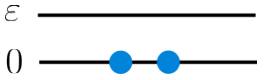
\includegraphics[width=0.25\linewidth]{Immagini/sistema a due livelli bosoni (i).png}
    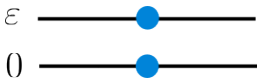
\includegraphics[width=0.25\linewidth]{Immagini/sistema a due livelli bosoni (ii).png}
    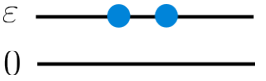
\includegraphics[width=0.25\linewidth]{Immagini/sistema a due livelli bosoni (iii).png}
    \caption{microstati: (i) $\ket{\nu}_1$; (i) $\ket{\nu}_2$; (i) $\ket{\nu}_3$.}
    \label{fig: sistema a due livelli bosoni}
\end{figure}
\paragraph{Fermioni.} Se le particelle sono fermioni, allora esiste un solo microstato possibile, mostrato in figura \ref{fig: sistema a due livelli fermioni}, dato da
\begin{equation}
    \ket{\nu} = \frac{1}{\sqrt{2!}}(\ket{1}_1 \otimes \ket{0}_2 + \ket{0}_1 \otimes \ket{1}_2).
\end{equation}
La funzione di partizione corrispondente è
\begin{equation}
    Z_F = \nsum_\nu e^{-\beta E_\nu} = e^{-\beta\epsilon}.
\end{equation}
\begin{figure}[h]
    \centering
    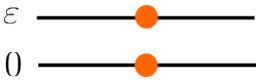
\includegraphics[width=0.25\linewidth]{Immagini/sistema a due livelli fermioni.png}
    \caption{l'unico microstato possibile per un sistema due livelli fermionico.}
    \label{fig: sistema a due livelli fermioni}
\end{figure}
\paragraph{Particelle distinguibili.} Per confronto, se si considerassero le particelle distinguibili, allora il numero di possibili microstati sarebbe quattro, mostrati in figura \ref{fig: sistema a due livelli classico}, e la funzione di partizione si fattorizzerebbe
\begin{equation}
    Z_D = |Z_{(1)}|^2 = (1 + e^{-\beta\epsilon})(1 + e^{-\beta\epsilon}) = 1 + 2e^{-\beta\epsilon} + e^{-2\beta\epsilon}.
\end{equation}
Confrontando $Z_D$ con $Z_B$ e $Z_F$, si nota come le interazioni statistiche non permettano alle funzioni di partizione bosonica e fermionica di fattorizzare; inoltre nel caso classico si era aggiunto il fattore di Gibbs per evitare l'omonimo paradosso, tuttavia se si segue questa strada si nota che
\begin{equation}
    Z_B \neq \frac{Z_D}{N!},\quad Z_F \neq \frac{Z_D}{N!}.
\end{equation}
\begin{figure}[h]
    \centering
    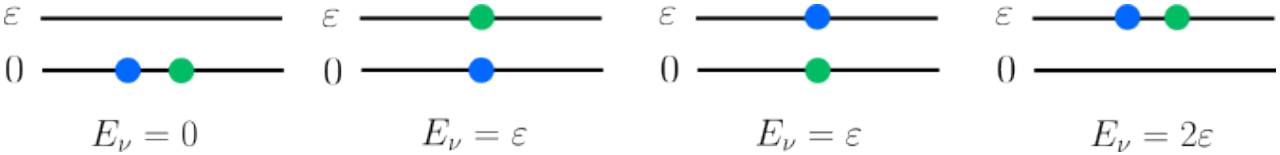
\includegraphics[width=0.95\linewidth]{Immagini/sistema a due livelli classico.png}
    \caption{possibili microstati per un sistema a due livelli classico.}
    \label{fig: sistema a due livelli classico}
\end{figure}
L'unico caso in cui vale l'uguaglianza le funzioni di partizione è quando le due particelle occupano livelli diversi. Dunque, il protocollo che si segue classicamente per evitare il paradosso di Gibbs è impreciso: vale solamente quando le componenti occupano tutte livelli differenti; tuttavia, nel caso del gas ideale, i livelli sono così densi che non succede praticamente mai che due particelle occupino lo stesso livello. 

\subsection{Coppia di particelle libere in una dimensione}
Si considerino due particelle in uno spazio unidimensionale con condizioni al contorno periodiche\footnote{Comunque, la generalizzazione tridimensionale, come anche l'inclusione delle condizioni di annullamento al bordo, non presenta particolari complicazioni.}. Per una singola particella, gli autostati di energia sono identificati da un numero
$m \in \Z$ con energia
\begin{equation}
    \epsilon_m = \frac{\hbar^2}{2m} \left( \frac{2\pi}{L} \right)^2 m^2,
\end{equation}
mentre per $N = 2$ particelle i possibili microstati bosonici $\ket{\nu_B}$ e fermionici $\ket{\nu_F}$ sono
identificati come 
\begin{equation}
\nu_B \longleftrightarrow \{ m_1 \ge m_2 \}, \quad
\nu_F \longleftrightarrow \{ m_1 > m_2 \}
\end{equation}
con energie
\begin{equation}
E_{\nu_B} = E_{\nu_F}
= \frac{\hbar^2}{2m} \left( \frac{2\pi}{L} \right)^2 (m_1^2 + m_2^2).
\end{equation}
Usando il fatto che
\begin{equation}
    \frac{\beta \pi^2}{2m} \left( \frac{2\pi}{L} \right)^2 = \frac{\pi \lambda_T^2}{L^2}
\end{equation}
la funzione di partizione bosonica risulta essere
\begin{equation}
    Z_B = \sum_{m_1 \ge m_2 \in \mathbb{Z}}e^{-\pi \lambda_T^2(m_1^2 + m_2^2)/L^2},
\end{equation}
dove la somma si può essere riorganizzata come
\begin{equation}
    \sum_{m_1 \ge m_2} = \frac{1}{2}
\bigg( \sum_{m_1, m_2} + \sum_{m_1 = m_2} \bigg),
\end{equation}
in questo modo l'espressione esatta della funzione di partizione bosonica diventa
\begin{equation}
    \begin{split}
        Z_B &= \frac{1}{2} \bigg( \sum_{m_1,m_2 \in \mathbb{Z}} e^{-\lambda_T^2(m_1^2+m_2^2)\pi/L^2} + \sum_{m \in \mathbb{Z}} e^{-2\lambda_T^2 m^2\pi/L^2} \bigg) \\
        &= \frac{1}{2} \bigg\{\bigg[\theta_3\bigg(\frac{i\lambda_T^2}{L^2}\bigg)\bigg]^2 + \theta_3\bigg(\frac{2i\lambda_T^2}{L^2}\bigg)\bigg\}.
    \end{split}
\end{equation}
Nel limite termodinamico $\lambda_T \ll L$ si ha
\begin{equation}
    Z_B = \frac{1}{2} \bigg[ \bigg( \frac{L}{\lambda_T} \bigg)^2 \left( 1 + 2 e^{-\pi L^2/\lambda_T^2} + \cdots \right) + \frac{L}{\sqrt{2}\lambda_T} \bigg( 1 + 2 e^{-\pi L^2/2\lambda_T^2} + \cdots \bigg) \bigg],
\end{equation}
ossia a meno di termini esponenzialmente soppressi
\begin{equation}
\label{eq: funzione di partizione bosonica sistema 2 particelle libere 1-dim}
    Z_B \simeq \frac{1}{2!} \bigg( \frac{L}{\lambda_T} \bigg)^2 \bigg( 1 + \frac{\lambda_T}{\sqrt{2}\,L} + \cdots \bigg),
\end{equation}
dove compaiono delle correzioni dovute ad interazioni statistiche create dall'indistinguibilità quantistica.
\begin{obs}
    Il risultato ottenuto nella \eqref{eq: funzione di partizione bosonica sistema 2 particelle libere 1-dim} è quello che si otterrebbe rimpiazzando le somme con integrali secondo
    \begin{equation}
        \frac{1}{2} \bigg( \sum_{m_1,m_2} + \sum_{m_1=m_2} \bigg) = \frac{1}{2}\bigg[\bigg( \frac{L}{2\pi} \bigg)^2 \int dk_1\, dk_2 + \frac{L}{2\pi} \int_{k_2=k_1} dk_1\bigg]
    \end{equation}
\end{obs}
Invece, la funzione di partizione fermionica è
\begin{equation}
    Z_F = \sum_{m_1>m_2} e^{-\lambda_T^2(m_1^2+m_2^2)/L^2},
\end{equation}
che sfruttando la riorganizzazione della somma seguente
\begin{equation}
    \sum_{m_1>m_2} = \frac{1}{2} \bigg( \sum_{m_1,m_2} - \sum_{m_2=m_1} \bigg)
\end{equation}
si procede con il conto esattamente come nel caso bosonico, arrivando all'espressione
\begin{equation}
\label{eq: funzione di partizione fermionica sistema 2 particelle libere 1-dim}
    Z_F = \frac{1}{2} \bigg\{\bigg[\theta_3\bigg(\frac{i\lambda_T^2}{L^2}\bigg)\bigg]^2 - \theta_3\bigg(\frac{2i\lambda_T^2}{L^2}\bigg)\bigg\} \simeq \frac{1}{2!} \bigg( \frac{L}{\lambda_T} \bigg)^2 \bigg( 1 - \frac{\lambda_T}{\sqrt{2}\,L} + \cdots \bigg)
\end{equation}

\subsection{Matrice densità}
Anche tramite il formalismo della matrice densità per i sistemi non interagenti emergono delle interazioni statistiche tra le componenti del sistema. Invece che rappresentare la matrice densità nella base dell'energia, in questo caso si sceglie la base delle posizioni; in ogni caso, la trattazione seguente è indipendente dalla scelta della base. Si indica quindi con $\{\ket{x}\}$ una base di stati della singola componente nella base degli autostati di posizione, per cui la funzione d'onda dello stato stazionario $\ket{a}$ è data da
\begin{equation}
    u_a(x) \equiv \mybraket{x}{a}.
\end{equation}
Per il sistema di $N$ componenti si indica la base degli autostati di posizione con
\begin{equation}
    \ket{x_1,\dots,x_N} = \ket{x_1}_1 \otimes \cdots \otimes \ket{x_N}_N.
\end{equation}
Se $\ket{\nu}$ è un stato stazionario, definito dalla \eqref{eq: microstato invariante per permutazioni}, la funzione d'onda $u_\nu$ associata è
\begin{equation}
    u_\nu \equiv \mybraket{x_1,\dots,x_N}{\nu} = \norm_\nu\nsum_P\delta_P\mybraket{x_1}{a_{P(1)}}\cdots\mybraket{x_N}{a_{P(N)}},
\end{equation}
dove il fattore di normalizzazione $\norm_\nu$ è sempre dato dalla \eqref{eq: normalizzazione microstati sistemi non interagenti identici}. Considerando che
\begin{equation}
\label{eq: proprietà produttoria}
    \nprod_if(i) = \nprod_if[P^{-1}(i)]
\end{equation}
dato che la permutazione riarrangia solamente l'ordine dei fattori, si può riscrivere $u_\nu$ tenendo fissi gli stati $\ket{a_i}$ e permutando le $x_i$, così da avere
\begin{equation}
    u_\nu = \norm_\nu\nsum_{P^{-1}}\delta_{P^{-1}}\mybraket{x_{P^{-1}(1)}}{a_1}\cdots\mybraket{x_{P^{-1}(N)}}{a_N}.
\end{equation}
Considerando che sommare su tutte le permutazioni $P$ o sugli inversi delle permutazioni $P^{-1}$ è equivalente, per cui
\begin{equation}
    \nsum_P \equiv \nsum_{P^{-1}},\quad \delta_P = \delta_{P^{-1}}
\end{equation}
è quindi possibile scrivere 
\begin{equation}
\label{eq: funzione onda sistemi non interagente identico}
    \begin{split}
        u_\nu &= \norm_\nu\nsum_P\delta_P\mybraket{x_{P(1)}}{a_1}\cdots\mybraket{x_{P(N)}}{a_N} \\
        &= \norm_\nu\nsum_P\delta_Pu_{a_1}[x_{P(1)}]\cdots u_{a_N}[x_{P(N)}].
    \end{split}
\end{equation}
Quindi, la matrice densità canonica è data da
\begin{equation}
    \rho(x_1,\dots,x_N;y_1,\dots,y_N) = \mybrakett{x_1,\dots,x_N}{\frac{e^{-\beta\hatH}}{Z}}{y_1,\dots,y_N}.
\end{equation}
Inserendo una relazione di completezza $\nsum_\nu\ket{\nu}\bra{\nu} = \MI$ nella definizione di $\rho(x_i;y_i) \equiv \rho(x_1,\dots,x_N;y_1,\dots,y_N)$, segue che 
\begin{equation}
    \begin{split}
        \rho(x_i;y_i) &= \frac{1}{Z}\nsum_\nu\mybraket{x_1,\dots,x_N}{\nu}\mybraket{\nu}{y_1,\dots,y_N}e^{-\beta E_\nu} \\
        &= \frac{1}{Z}\nsum_\nu u_\nu^*(y_1,,\dots,y_N)u_{\nu}(x_1,\dots,x_N)e^{-\beta E_\nu} \\
        &= \frac{1}{Z}\nsum_\nu|\norm_\nu|^2\nsum_{P,Q}\delta_P\delta_Qu_{a_1}^*[y_{P(1)}]u_{a_1}[x_{Q(1)}]\\
        &\times\cdots\times u_{a_N}^*[y_{P(N)}]u_{a_N}[x_{Q(N)}]e^{-\beta(\epsilon_{a_1}+\cdots+\epsilon_{a_N})} \\
        &= \frac{1}{Z}\nsum_\nu|\norm_\nu|^2\nsum_{P,Q}\delta_P\delta_Qu_{a_1}^*[y_{PQ^{-1}(1)}]u_{a_1}(x_1)\\
        &\times\cdots\times u_{a_N}^*[y_{PQ^{-1}(N)}]u_{a_N}(x_N)e^{-\beta(\epsilon_{a_1}+\cdots+\epsilon_{a_N})},
    \end{split}
\end{equation}
dove nel penultimo e nell'ultimo passaggio si sono usate rispettivamente le equazioni \eqref{eq: funzione onda sistemi non interagente identico} e \eqref{eq: proprietà produttoria}. Dato che una delle permutazioni è ridondante si riduce ad un fattore $N!$, inoltre ponendo $R \equiv PQ^{-1}$ si ha $\delta_P\delta_Q = \delta_P\delta_{Q^{-1}} \equiv \delta_R$ e mappando la somma sui microstati con quella che conta sugli stati $a_i$ ordinati, per cui si ottiene
\begin{equation}
    \begin{split}
        \rho(x_i,y_i) = \frac{1}{Z}\nsum_\nu|\norm_\nu|^2\nsum_Pf(\{a_i\}) &= \frac{N!}{Z}\nsum_\nu|\norm_\nu|^2f(\{a_i\}) \\
        &= \frac{1}{Z}\sum_{a_1\ge\cdots\ge a_N}\frac{f(\{a_i\})}{\nprod_a n_a!},
    \end{split}
\end{equation}
dove si sostituita l'espressione del fattore di normalizzazione \eqref{eq: normalizzazione microstati sistemi non interagenti identici} e si è posta la funzione $f(\{a_i\})$ del microstato invariante (a meno di un segno globale nel caso fermionico) per permutazioni delle $a_i$ come
\begin{equation}
    f(\{a_i\}) \equiv \nsum_{R}\delta_Ru_{a_1}^*[y_{R(1)}]u_{a_1}(x_1)\cdots u_{a_N}^*[y_{R(N)}]u_{a_N}(x_N)e^{-\beta(\epsilon_1+\cdots+\epsilon_N)};
\end{equation}
inoltre, notando che la sommatoria ordinata si può scrivere senza vincoli sull'ordinamento stesso, in termini della somma indipendente su tutti gli stati $a_i$ si ha
\begin{equation}
    \begin{split}
        \rho(x_i,y_i) &= \frac{1}{N!Z}\sum_{a_1,\cdots,a_N}f(\{a_i\}) \\
        &= \frac{1}{N!Z}\sum_{a_1,\cdots,a_N}\nsum_{R}\delta_Ru_{a_1}^*[y_{R(1)}]u_{a_1}(x_1)\\
        &\times\cdots\times u_{a_N}^*[y_{R(N)}]u_{a_N}(x_N)e^{-\beta(\epsilon_1+\cdots+\epsilon_N)} \\
        &= \frac{1}{N!Z}\nsum_{R}\delta_R\nsum_{a_1}u_{a_1}^*[y_{R(1)}]u_{a_1}(x_1)e^{-\beta\epsilon_{a_1}}\\
        &\times\cdots\times\nsum_{a_N}u_{a_N}^*[y_{R(N)}]u_{a_N}(x_N)e^{-\beta\epsilon_N},
    \end{split}
\end{equation}
da cui in definitiva, riconoscendo in ogni somma indipendente sugli stati $a_i$ le matrici densità di singola particella mancanti della normalizzazione $1/Z_{(1)}$, si ottiene
\begin{equation}
\label{eq: matrice densità sistemi non interagenti identici}
    \rho(x_1,\dots,x_N;y_1,\dots,y_N) = \frac{[Z_{(1)}]^N}{N!Z}\nsum_R\delta_R\rho[x_1,y_{R(1)}]\cdots\rho[x_N,y_{R(N)}].
\end{equation}
La statistica entra in gioco ``mescolando'' i termini. L'equazione \eqref{eq: matrice densità sistemi non interagenti identici} mostra come siano presenti delle ``interazioni statistiche'' tra le varie componenti pur non avendo termini di interazioni nell'hamiltoniana del sistema in quanto la matrice densità non è fattorizzata nelle varie componenti. 

\subsection{\texorpdfstring{$N$}{N} particelle libere in tre dimensioni}
Sfruttando il formalismo della matrice densità, in questo caso si ha
\begin{equation}
    \rho(\vx_i,\vx_j) = \frac{1}{V}\exp{\bigg(-\frac{\prod_{i,j}|\vx_i - \vx_j|^2}{\lambda_T^2}\bigg)} \equiv \frac{f_{ij}}{V}.
\end{equation}
Usando la relazione \eqref{eq: funzione di partizione singola particella (canonico)} per la funzione di partizione di singola particelle $Z_{(1)}$ si può scrivere
\begin{equation}
\label{eq: matrice densità sistemi non interagenti identici N particelle 3-dim}
    \begin{split}
        Z\rho(\vx_i,\vx_j) &= \frac{1}{N!}\bigg(\frac{V}{V_T}\bigg)^N\nsum_P\delta_P\frac{f_{1,P(1)}}{V}\cdots\frac{f_{N,P(N)}}{V} \\
        &= \frac{1}{V_T^NN!}\nsum_P\delta_Pf_{1,P(1)}\cdots f_{N,P(N)}.
    \end{split}
\end{equation}
Si nota che per i termini diagonali della matrice densità, i quali codificano la probabilità di trovare il sistema con determinate posizioni, si ha $f_{ii} = 1$; quindi, per ogni permutazione $P$ nella somma a secondo membro della \eqref{eq: matrice densità sistemi non interagenti identici N particelle 3-dim} ogni coordinata lasciata invariata da $P$ contribuisce con un fattore pari a $1$. Pertanto, si ha un termine non banale solo per le coordinate che vengono permutate. Integrando la \eqref{eq: matrice densità sistemi non interagenti identici N particelle 3-dim} sulle coordinate $\vx_1,\dots,\vx_N$ si ottiene la funzione di partizione $Z$ dato che la matrice densità è normalizzata ad uno per costruzione. Dunque, si ha
\begin{equation}
\label{eq: funzione di partizione sistemi non interagenti identici N particelle 3-dim}
    Z = \frac{1}{V_T^NN!}\nsum_P\delta_P\int d^3x_1\cdots d^3x_N\,f_{1,P(1)}\cdots f_{N,P(N)}.
\end{equation}
Nella funzione di partizione \eqref{eq: funzione di partizione sistemi non interagenti identici N particelle 3-dim} le variabili $\vx_i$ sono integrate, ossia mute, per cui l'etichetta delle $x$ non è rilevante: se si riordinassero le $\vx$ tra di loro non cambierebbe nulla; in altre parole, tutte le permutazioni appartenenti alla stessa classe di coniugazione ($[P] = \{Q^{-1}PQ\},\,Q\in S_n$) restituiscono lo stesso contributo. 
\paragraph{Classe dell'identità.} La classe di coniugazione dell'identità contiene solo l'identità
\begin{equation}
    P = \MI \to \int d^3x_1\cdots d^3x_N\,f_{1,1}\cdots f_{N,N} = \int d^3x_1\cdots d^3x_N = V^N.
\end{equation}
\paragraph{Classe degli scambi $i\leftrightarrow j$.} La classe di coniugazione degli scambi contiene le permutazioni $P$ che lasciano fissi $(N-2)$ elementi e
ne scambiano due fra di loro. Quindi, nell'integrale si hanno $f_{12}$, $f_{21}$ e da $f_{33}$ in poi si hanno tutti termini uguali pari ad $1$. Per queste permutazioni $\delta_P = \pm 1$ per bosoni o fermioni rispettivamente. Dunque, il numero di scambi è $\binom{N}{2}$, corrispondente alla scelta degli elementi scambiati. 
\begin{ex}
    Per lo scambio $(1 \leftrightarrow 2)$ si ottiene
    \begin{multline}
    \label{eq: permutazione scambio 1 - 2}
        \int d^3 x_1 d^3 x_2\,f_{12} f_{21} \int d^3 x_3 \cdots d^3 x_N\,1 \cdot 1 \cdots =\\
        = V^{N-2} \int d^3 x_1 \int d^3 x_2\,\exp\bigg[{- \frac{\pi}{\lambda_T^2} (|\vx_{12}|^2 + |\vx_{21}|^2)}\bigg],
    \end{multline}
    dove $|\vx_{12}|^2 + |\vx_{21}|^2
        = 2\, |\vx_{12}|^2$. Ora, con il cambio di variabili dato da
    \begin{equation}
        \begin{cases}
            \vx_{CM} = \dfrac{1}{2}(\vx_1 + \vx_2) \\[2ex]
        \vz \equiv \vx_{12} = \vx_1 - \vx_2
        \end{cases}
    \end{equation}
    avente jacobiano pari a $1$, la \eqref{eq: permutazione scambio 1 - 2} diventa
    \begin{equation}
        V^{N-2} \int d^3 x_{CM} \int d^3 z \, \exp{\bigg(-\frac{2\pi}{\lambda_T^2}|z|^2\bigg)} = V^{N-2} V \bigg( \frac{\lambda_T^2}{2} \bigg)^{3/2} =  \frac{V_T}{V} \frac{V^N}{2^{3/2}}
    \end{equation}
\end{ex}

\subsubsection{Limite di alta temperatura}
Nel limite di alta temperatura per cui $V_T \ll V$, le classi di permutazioni che contengono più di uno scambio sono ulteriormente soppresse in quanto contengono potenze più alte di $V_T/V$. Dunque, si può ridurre la funzione di partizione \eqref{eq: funzione di partizione sistemi non interagenti identici N particelle 3-dim} all'espressione
\begin{equation}
    Z = \frac{1}{N!}\bigg(\frac{V}{V_T}\bigg)^N\bigg[1 + \binom{N}{2}\frac{V_T}{2^{3/2}V} + \cdots \bigg],
\end{equation}
la quale rappresenta una generalizzazione per un sistema di $N$ particelle in uno spazio tridimensionale delle funzioni di partizione bosonica \eqref{eq: funzione di partizione bosonica sistema 2 particelle libere 1-dim} e fermionica \eqref{eq: funzione di partizione fermionica sistema 2 particelle libere 1-dim}. La coda di correzioni dovute alle permutazioni non banali, soppresse dal limite di alta temperatura $V_T/V$, sono, come già detto, un effetto di interazione di natura statistica. Queste interazioni possono diventare significative e dare luogo a comportamenti non banali di $Z$, e quindi delle grandezze termodinamiche, nel regime di bassa temperatura in cui $V_T$ diviene comparabile o superiore a $V$.

\subsubsection{Considerazioni}
Riassumendo quanto fatto, il modo più immediato per scrivere la funzione di partizione nell'ensemble canonico consiste nel caratterizzare gli stati tramite il formalismo dei numeri di occupazione, in particolare
\begin{equation}
    \ket{\nu} \longleftrightarrow \{n_a\} : \nsum_a n_a = N,\quad n_a \in 
    \begin{cases}
        \N_0\,\mathrm{bosoni} \\
        \{0,1\} \,\mathrm{fermioni}
    \end{cases},
\end{equation}
in termini dei quali l'energia dei microstati è $E_\nu = \nsum_a n_a\epsilon_a$, risultando quindi in una funzione di partizione della forma
\begin{equation}
    Z= \nsum_\nu e^{-\beta E_\nu} = \nsum_{\{n_a\}}e^{-\beta\nsum_an_a\epsilon_a}.
\end{equation}
Per un generico sistema con $N$ elevato, la presenza del vincolo $\nsum_a n_a = N$ nella sommatoria rende complesso determinare $Z$. Sarebbe più semplice se si potesse fare una somma indipendente: se si sommasse su $n_a$ senza avere il vincolo su $N$, si otterrebbe un sistema aperto. Per questa ragione, risulta conveniente trattare i gas ideali quantistici nell'ensemble grancanonico.
\chapter{Ensemble grancanonico}
Si consideri un sistema $A$ non isolato e aperto, immerso in un ambiente $B$ molto più grande che funge da bagno termico e chimico, come mostrato in figura \ref{fig: sistema generico (grancanonico)}. In questo sistema, l'equilibrio viene sempre raggiunto alla temperatura $T$ e al potenziale chimico $\mu$ dell'ambiente $B$.
\begin{figure}[h]
    \centering
    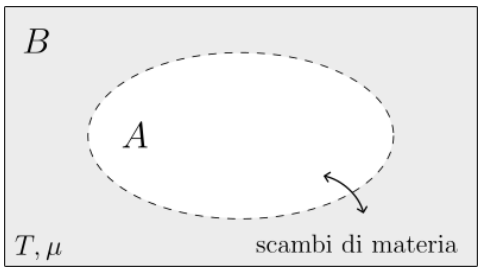
\includegraphics[width=0.4\linewidth]{Immagini/sistema generico (grancanonico).png}
    \caption{sistema generico per l'ensemble grancanonico.}
    \label{fig: sistema generico (grancanonico)}
\end{figure}
Per determinare la distribuzione di probabilità del sistema $A$ all'equilibrio si procede con il massimizzare il funzionale di entropia di Gibbs \eqref{eq: definizione entropia Gibbs} tenendo conto dei seguenti vincoli:
\begin{enumerate}
    \item la probabilità è normalizzata da $\nsum_\nu P(\nu) = 1$;
    \item l'energia dei microstati può fluttuare, ma l'energia media va fissata ad un valore $E$ che, nel limite termodinamico, coincide con l'energia termodinamica, ossia $\vmedio{E} = \nsum_\nu P(\nu)E(\nu) \equiv E$;
    \item il numero di particelle può fluttuare, ma il valor medio va fissato ad un valore $N$ che rappresenta il valore termodinamico di $N$, ossia $\vmedio{N} = \nsum_\nu P(\nu)N(\nu) \equiv N$. 
\end{enumerate}
In modo analogo a quanto fatto per gli ensemble microcanonico e canonico, si introduce per ogni vincolo un moltiplicatore di Lagrange e si massimizza il funzionale di entropia dato da
\begin{equation}
    \begin{split}
        \tilde{\SG}[P] &= \SG[P] + \alpha_0\bigg(\nsum_\nu P(\nu) - 1\bigg) + \alpha_E\bigg(\nsum_\nu P(\nu)E(\nu) - E\bigg) \\
        &+ \alpha_N\bigg(\nsum_\nu P(\nu)N(\nu) - N\bigg)
    \end{split}
\end{equation}
imponendo $\delta\tilde{\SG}[P] = 0$, ossia
\begin{multline}
     \delta\bigg[-k\nsum_\nu P(\nu)\log{P(\nu)} + \alpha_0\bigg(\nsum_\nu P(\nu) - 1\bigg) + \\
     + \alpha_E\bigg(\nsum_\nu P(\nu)E(\nu) - E\bigg) + \alpha_N\bigg(\nsum_\nu P(\nu)N(\nu) - N\bigg)\bigg] = 0.
\end{multline}
Rispetto a variazioni arbitrarie $\delta P(\nu)$ si ha
\begin{equation}
    \nsum_\nu\delta P(\nu)[-k\log{P(\nu)} - k + \alpha_0 + \alpha_EE(\nu) + \alpha_NN(\nu)] = 0,
\end{equation}
da cui, ponendo il termine in parentesi quadra tra parentesi a zero, si ottiene
\begin{equation}
    P(\nu) = \exp{\bigg(-1 + \frac{\alpha_0}{k}\bigg)}\exp{\bigg(\frac{\alpha_E}{k}E(\nu) + \frac{\alpha_E}{k}N(\nu)\bigg)}.
\end{equation}
Imponendo adesso il primo vincolo e ponendo $\exp{(-1 + \alpha_0/k)} \equiv 1/Q$, viene fissato $\alpha_0$ e si ha
\begin{equation}
    \nsum_\nu P(\nu) = \frac{1}{Q}\nsum_\nu \exp{\bigg(\frac{\alpha_E}{k}E(\nu) + \frac{\alpha_E}{k}N(\nu)\bigg)},
\end{equation}
da cui 
\begin{equation}
    Q = \nsum_\nu \exp{\bigg(\frac{\alpha_E}{k}E(\nu) + \frac{\alpha_E}{k}N(\nu)\bigg)},
\end{equation}
mentre il funzionale di entropia diventa
\begin{equation}
    \SG[P] = -k\nsum_\nu P(\nu) \log{P(\nu)} = -k \nsum_\nu P(\nu)\bigg[\frac{\alpha_E}{k}E(\nu) + \frac{\alpha_N}{k}N(\nu) - \log{Q}\bigg].
\end{equation}
Imponendo il secondo e il terzo vincolo, si deduce che $\vmedio{E}$ e $\vmedio{N}$ vanno interpretate come l'energia e il numero di componenti termodinamici 
\begin{equation}
\label{eq: entropia di Gibbs (grancanonico)}
    \SG[P] = -\alpha_E\vmedio{E} - \alpha_N\vmedio{N} + k\log{Q},
\end{equation}
per cui devono valere le equazioni di stato termica e chimica \eqref{eq: equazioni di stato da S} date da
\begin{equation}
\label{eq: equazioni di stato grancanonico}
    \frac{\p S}{\p E}\bigg|_{V,N} = \frac{1}{T} = -\alpha_E,\quad \frac{\p S}{\p N}\bigg|_{E,V} = -\frac{\mu}{T} = -\alpha_N.
\end{equation}
In definitiva, si trova che 
\begin{equation}
    P(\nu) = \frac{1}{Q}\exp{\bigg(-\frac{1}{kT}E(\nu) + \frac{\mu}{kT}N(\nu)\bigg)} = \frac{1}{Q}e^{-\beta[E(\nu) - \mu N(\nu)]},
\end{equation}
dove $Q$ è la funzione di partizione grancanonica
\begin{equation}
\label{eq: funzione di partizione grancanonica}
    Q = \nsum_\nu e^{-\beta[E(\nu) - \mu N(\nu)]}.
\end{equation}
Si ricorda che $\mu$ è l'energia interna termodinamica associata ad ogni singolo componente, quindi solo per il fatto di avere $N$ componenti nel sistema, si ha un certo costo energetico $N\mu$ contenuto nell'energia termodinamica interna. La probabilità grancanonica distribuisce esponenzialmente gli stati in base alla differenza tra $E(\nu)$ e l'energia dovuta al potenziale chimico $\mu N$, quindi
\begin{equation}
    P(\nu) \propto e^{-\beta[E(\nu) - \mu N(\nu)]}.
\end{equation}
Inoltre, risulta spesso conveniente utlizzare la fugacità $z$ che permette di passare dalla coppia di variabili intensive indipendenti $(T,\mu)$ alla coppia di variabili $(T,z)$ 
\begin{equation}
    z \equiv e^{\beta\mu},
\end{equation}
legando il costo di aggiungere e togliere particelle alla scala di energia termica. In questi termini si hanno
\begin{equation}
    P(\nu) = \frac{1}{Q}z^{N(\nu)}e^{-\beta E(\nu)},\quad Q = \nsum_\nu z^{N(\nu)}e^{-\beta E(\nu)}.
\end{equation}
Sostituendo le equazioni di stato \eqref{eq: equazioni di stato grancanonico} nella \eqref{eq: entropia di Gibbs (grancanonico)} si ha
\begin{equation}
    S = \frac{E}{T} - \frac{\mu N}{T} + k\log{Q},
\end{equation}
da cui, moltiplicando per $T$ e riarrangiando i termini, si ottiene l'espressione del potenziale grancanonico 
\begin{equation}
    \varpi(T,V,\mu) = -kT\log{Q(T,V,\mu)} = - \frac{1}{\beta} \log{Q(T,V,\mu)},
\end{equation}
punto di partenza per determinare la termodinamica dell'ensemble grancanonico. Pertanto la funzione di partizione grancanonica $Q$ si può esprimere in funzione di $\varpi$ come
\begin{equation}
    Q(T,V,\mu) = e^{-\beta\varpi(T,V,\mu)}.
\end{equation}
Per quanto riguarda l'energia interna, questa è data da
\begin{equation}
    \begin{split}
        \vmedio{E} = \varpi + TS +\mu N &= \varpi + \beta\frac{\p\varpi}{\p\beta}\bigg|_{V,\mu} - \mu\frac{\p\varpi}{\p\mu}\bigg|_{T,V} \\
        &= \frac{\p}{\p\beta}(\beta\varpi)\bigg|_{V,\mu} - \mu\frac{\p\varpi}{\p\mu}\bigg|_{T,V};
    \end{split}
\end{equation}
invece, in termini della fugacità, si può esprimere $\vmedio{N}$ come
\begin{equation}
\label{eq: numero medio N (grancanonico)}
    \begin{split}
        \vmedio{N} = \frac{1}{Q}\nsum_\nu N(\nu)z^{N(\nu)}e^{-\beta E(\nu)} = \frac{z}{Q}\frac{\p Q}{\p z}\bigg|_{T,V} 
        &= z\frac{\p\ln{Q}}{\p z}\bigg|_{T,V} \\ 
        &= -\beta z\frac{\p\varpi}{\p z}\bigg|_{T,V}.
    \end{split}
\end{equation}
La densità è definita come l'inverso del volume per particella $v$, quindi 
\begin{equation}
    \frac{1}{v} = \frac{N}{V} = -\frac{\beta z}{V}\frac{\p\varpi}{\p z}\bigg|_{T,V}.
\end{equation}
Inoltre, l'energia media può venire espressa, in termini della fugacità, come
\begin{equation}
\label{eq: numero medio E (grancanonico)}
    \begin{split}
        \vmedio{E} = \frac{1}{Q}\nsum_\nu z^{N(\nu)}e^{-\beta E(\nu)}E(\nu) = -\frac{1}{Q}\frac{\p Q}{\p\beta}\bigg|_{V,z} &= -\frac{\p\log{Q}}{\p\beta}\bigg|_{V,z} \\
        &= \frac{\p}{\p\beta}(\beta\varpi)\bigg|_{V,z}.
    \end{split}
\end{equation}

\subsubsection{Fluttuazioni dell'energia e del numero di particelle}
In analogia a quanto visto per l'ensemble microcanonico, si può mostrare che le varianze $\sigma^2_E$ e $\sigma_N^2$ nel limite termodinamico sono estensive
\begin{equation}
    \sigma_E^2 = \vmedio{E^2} - \vmedio{E}^2 \propto N,\quad \sigma_N^2 = \vmedio{N^2} - \vmedio{N}^2 \propto N,
\end{equation}
per cui le fluttuazioni relative in questo limite seguono un  andamento del tipo
\begin{equation}
    \frac{\sigma_E}{\vmedio{E}} \propto \frac{1}{\sqrt{N}}, \quad \frac{\sigma_N}{\vmedio{N}} \propto \frac{1}{\sqrt{N}}.
\end{equation}

\subsubsection{Relazione tra $Q$ e $Z$}
Nella definizione della funzione di partizione grancanonica \eqref{eq: funzione di partizione grancanonica} è possibile partizionare la somma sui microstati $\nu$ raggruppandoli in base al numero di particelle $N(\nu)$. Quindi, si ha
\begin{equation}
     \begin{split}
         Q = \nsum_N\nsum_{\nu_N} e^{-\beta E(\nu_N)}e^{\beta\mu N(\nu_N)} &= \nsum_Ne^{\beta\mu N}\nsum_{\nu_N}e^{-\beta E(\nu_N)} \\
         &= \nsum_Nz^N\nsum_{\nu_N}e^{-\beta E(\nu)},
     \end{split}
\end{equation}
dato che $z$ è costante per tutti i microstati. La sommatoria $\nsum_{\nu_N}$ rappresenta la funzione di partizione $Z_{(N)}$ per l'ensemble con $N$ componenti. In termini della fugacità, la funzione di partizione $Q$ diventa
\begin{equation}
\label{eq: funzione di partizione grancanonica (fugacità)}
    Q = \nsum_N z^NZ_{(N)}.
\end{equation}
Dunque, la funzione di partizione grancanonica può essere interpretata come la funzione generatrice\footnote{Con funzione generatrice in generale si intende una funzione da cui è possibile ottenere altre funzioni di interesse tramite un'espansione in serie rispetto a variabili ausiliarie.} delle funzioni di partizioni canoniche $Z_{(N)}$. 
\chapter{Statistica bosonica e fermionica}
Si consideri prima di tutto un sistema classico di particelle identiche non interagenti la cui funzione di partizione, tenendo conto del fattore di Gibbs, è data da
\begin{equation}
    Z_{(N)} = \frac{1}{N!}Z_{(1)}^N, \quad Z_{(1)} = \nsum_{a}e^{-\beta\epsilon_a} \equiv \nsum_\epsilon e^{-\beta\epsilon}.
\end{equation}
Usando l'espressione \eqref{eq: funzione di partizione grancanonica (fugacità)}, la funzione di partizione grancanonica è data da
\begin{equation}
    Q_{C} = \nsum_Nz^NZ_{(N)} = \nsum_N\frac{1}{N!}(zZ_{(1)})^N = e^{zZ_{(1)}},
\end{equation}
per cui il potenziale grancanonico è
\begin{equation}
    \varpi_{C} = -\frac{\log{Q_{C}}}{\beta} = -\frac{z}{\beta}Z_{(1)}.
\end{equation}
Usando la \eqref{eq: numero medio N (grancanonico)}, si può ricavare il numero medio di componenti 
\begin{equation}
    \vmedio{N}_{C} = zZ_{(1)} = \nsum_\epsilon ze^{-\beta\epsilon} = \nsum_\epsilon e^{-\beta(\epsilon - \mu)}.
\end{equation}
D'altra parte, il numero medio di componenti è anche determinato dalla somma del numero medio di particelle $n(\epsilon)$ in ogni livello $\epsilon$, per cui
\begin{equation}
    \vmedio{N}_{C} = \nsum_\epsilon \vmedio{n(\epsilon)}_{C}.
\end{equation}
Dal confronto di queste due espressioni per $\vmedio{N}_{C}$ è immediato trovare che
\begin{equation}
    \vmedio{n(\epsilon)}_{C} = e^{-\beta(\epsilon - \mu)} = ze^{-\beta\epsilon}.
\end{equation}
Dunque, secondo l'approccio classico il valore medio del numero di particelle per livello decresce in maniera esponenziale. 

\section{Gas ideale di bosoni}
Si consideri ora il medesimo sistema di particelle identiche non interagenti ma descritto tramite l'approccio quantistico supponendo che le componenti di tale sistema siano bosoni. In questo caso, ogni microstato $\nu$ è caratterizzato solamente da quante particelle in ciascuno dei possibili livelli di energia $\epsilon$ del singolo componente, indipendentemente da quali di queste; quindi, $\nu$ è determinato dai numeri di occupazione $n(\epsilon)$, con $n(\epsilon) \in \N_0$, senza alcuna limitazione in quanto il numero totale di componenti nell'ensemble grancanonico non è fissato. L'energia $E(\nu)$ del microstato $\nu$ è data da
\begin{equation}
    E(\nu) = \nsum_\epsilon n(\epsilon)\epsilon,\quad N(\nu) = \nsum_\epsilon n(\epsilon).
\end{equation}
Quindi, la funzione di partizione grancanonica bosonica $Q_B$ è data da\footnote{Dove la somma $\nsum_{n_i = 0}^\infty$ indica quante particelle popolano il livelli $i$-esimo.}
\begin{equation}
    \begin{split}
        Q_B = \nsum_\nu e^{-\beta[E(\nu) - \mu N(\nu)]} &= \bigg(\sum_{n_0 = 0}^\infty\sum_{n_1 = 0}^\infty \cdots\bigg)e^{-\beta\nsum_an_a(\epsilon_a - \mu)} \\
        &= \sum_{n_0 = 0}^\infty e^{-\beta n_0(\epsilon_0 - \mu)}\sum_{n_1 = 1}^\infty e^{-\beta n_1(\epsilon_1 - \mu)}\cdots \\
        &= \nprod_a\bigg(\sum_{n_a = 0}^\infty e^{-\beta n_a(\epsilon_a - \mu)}\bigg).
    \end{split}
\end{equation}
Adesso, sfruttando la definizione serie geometrica con ragione $e^{-\beta}$, si possono sommare le serie geometriche purché siano convergenti, ossia se la ragione è minore di uno; questo è il caso infatti
\begin{equation}
    \mu < \epsilon_a\quad\Longrightarrow\quad e^{-\beta(\epsilon_a - \mu)} < 1,\quad \forall a.
\end{equation}
In particolare, siccome $\epsilon_0 < \epsilon_1 < \cdots$, il potenziale chimico è limitato superiormente da $\mu < \epsilon_0$. Ad ogni modo, effettuando le somme in questione si arriva all'espressione
\begin{equation}
\label{eq: funzione di partizione grancanonica bosonica}
    Q_B = \frac{1}{1 - e^{-\beta(\epsilon_0 - \mu)}}\frac{1}{1 - e^{-\beta(\epsilon_1 - \mu)}}\cdots = \nprod_a\bigg(\frac{1}{1 - \epsilon^{-\beta(\epsilon_a - \mu)}}\bigg).
\end{equation}
Quindi, usando la definizione, il potenziale grancanonico è
\begin{equation}
    \varpi_B = \frac{1}{\beta}\nsum_a\log{[1 - \epsilon^{-\beta(\epsilon_a - \mu)}]} = \frac{1}{\beta}\nsum_\epsilon\log{(1 - ze^{-\beta\epsilon})}.
\end{equation}
Nel caso sia presente una degenerazione, e che quindi ci siano $g(\epsilon)$ stati degeneri nel livello $\epsilon$ i quali contribuiscono tutti in egual modo, allora l'espressione del potenziale grancanonico diventa
\begin{equation}
    \varpi_B = \frac{1}{\beta}\nsum_\epsilon g(\epsilon)\log{[1 - e^{-\beta(\epsilon - \mu)}]} = \frac{1}{\beta}\nsum_\epsilon g(\epsilon)\log{(1 - ze^{-\beta\epsilon})}.
\end{equation}
Conoscendo ora il potenziale, è possibile determinare il numero medio di componenti bosoniche da
\begin{equation}
    \begin{split}
        \vmedio{N}_B = -\beta z \frac{\p\varpi_B}{\p z}\bigg|_{T,V} &= -\nsum_\epsilon g(\epsilon)z\frac{\p}{\p z}\log{(1 - ze^{-\beta z})}\bigg|_{T,V} \\
        &= \nsum_\epsilon g(\epsilon)\frac{ze^{-\beta\epsilon}}{1 - ze^{-\beta\epsilon}} \\
        &= \nsum_\epsilon g(\epsilon)\frac{z}{e^{\beta\epsilon} - z},
    \end{split}
\end{equation}
che, confrontata con la solita definizione $\vmedio{N}_B = \nsum_\epsilon \vmedio{n(\epsilon)}_B$, restituisce la statistica di Bose - Einstein
\begin{equation}
\label{eq: statistica Bose-Einstein}
    \vmedio{n(\epsilon)}_B = g(\epsilon)\frac{z}{e^{\beta\epsilon} - z} = \frac{g(\epsilon)}{e^{\beta(\epsilon - \mu)} - 1}.
\end{equation}

\section{Gas ideale di fermioni}
In modo analogo al caso bosonico, nel caso di un sistema composto da particelle fermioniche non interagenti, il procedimento da seguire è essenzialmente il medesimo a meno del vincolo sui numeri di occupazione $n_a = \{0,1\}$ dovuto al principio di esclusione di Pauli. Quindi, in tal caso si arriva all'espressione
\begin{equation}
\label{eq: funzione di partizione grancanonica fermionica}
    \begin{split}
        Q_F &= \sum_{n_0 = 0}^1e^{-\beta n_0(\epsilon_0 - \mu)}\sum_{n_1 = 0}^1e^{-\beta n_1(\epsilon_1 - \mu)}\cdots \\
        &= [1 + e^{-\beta(\epsilon_0 - \mu)}][1 + e^{-\beta(\epsilon_1 - \mu)}]\cdots \\
        &= \nprod_a[1 + e^{-\beta(\epsilon_a - \mu)}].
    \end{split}
\end{equation}
Si nota che, a differenza del caso bosonico, le somme finite nell'espressione \eqref{eq: funzione di partizione grancanonica fermionica} non comportano alcune richiesta di convergenza, per cui non emerge alcuna condizione sul potenziale chimico $\mu$. Il potenziale grancanonico risulta essere
\begin{equation}
    \varpi_F = -\frac{1}{\beta}\nsum_a\log{[1 + e^{-\beta(\epsilon_a - \mu)}]} = -\frac{1}{\beta}\nsum_\epsilon \log{[1 + e^{-\beta(\epsilon - \mu)}]},
\end{equation}
che in presenza di degenerazione diventa
\begin{equation}
    \varpi_F = -\frac{1}{\beta}\nsum_\epsilon g(\epsilon)\log{[1 + e^{-\beta(\epsilon - \mu)}]} = -\frac{1}{\beta}\nsum_\epsilon g(\epsilon) \log{[1 + ze^{-\beta\epsilon}]}.
\end{equation}
Adesso, noto il potenziale, il numero medio di componenti fermioniche è dato da
\begin{equation}
    \begin{split}
        \vmedio{N}_F = -\beta z \frac{\p \varpi_F}{\p z}\bigg|_{T,V} &= \nsum_\epsilon g(\epsilon)\frac{\p}{\p z}\log{(1 + ze^{-\beta\epsilon})}\bigg|_{T,V} \\
        &= \nsum_\epsilon g(\epsilon)\frac{ze^{-\beta\epsilon}}{1 + ze^{-\beta\epsilon}} \\
        &= \nsum_\epsilon g(\epsilon)\frac{z}{e^{\beta\epsilon} + z},
    \end{split}
\end{equation}
il quale, confrontato con la definizione $\vmedio{N}_F = \nsum_\epsilon \vmedio{n(\epsilon)}_F$, restituisce la statistica di Fermi - Dirac
\begin{equation}
\label{eq: statistica Fermi-Dirac}
    \vmedio{n(\epsilon)}_F = g(\epsilon)\frac{z}{e^{\beta\epsilon} + z} = \frac{g(\epsilon)}{e^{\beta(\epsilon - \mu)} + 1}.
\end{equation}

\subsubsection{Confronto tra statistiche}
Per un generico livello $\epsilon$ di un sistema trattato secondo l'approccio classico e quantistico, distinguendo per quest'ultimo i casi di bosonico e fermionico, si hanno rispettivamente le seguenti statistiche 
\begin{align}
    \vmedio{n(\epsilon)}_{C} &= ze^{-\beta\epsilon} \\
    \vmedio{n(\epsilon)}_B &= \frac{g(\epsilon)}{e^{\beta(\epsilon - \mu)} - 1}, \\
    \vmedio{n(\epsilon)}_F &= \frac{g(\epsilon)}{e^{\beta(\epsilon - \mu)} + 1}.
\end{align}
Nel limite per il quale $z = e^{\beta\mu} \to 0$, si ha che tutte le statistiche tendono a coincidere $\vmedio{n(\epsilon)}_C \simeq \vmedio{n(\epsilon)}_B \simeq \vmedio{n(\epsilon)}_F$; pertanto tale limite corrisponde al limite classico, inoltre se $z \to 0$, allora si deve avere $\mu < 0$, con $|\mu| \gg kT$. Per qualsiasi livello $\epsilon$, l'andamento di $\vmedio{n(\epsilon)}$ delle diverse statistiche è riportato in figura \ref{fig: confronto statistiche}. Da quest'ultimo risulta evidente come a livello quantistico si presentino comportamenti differenti. 
\begin{figure}[h]
    \centering
    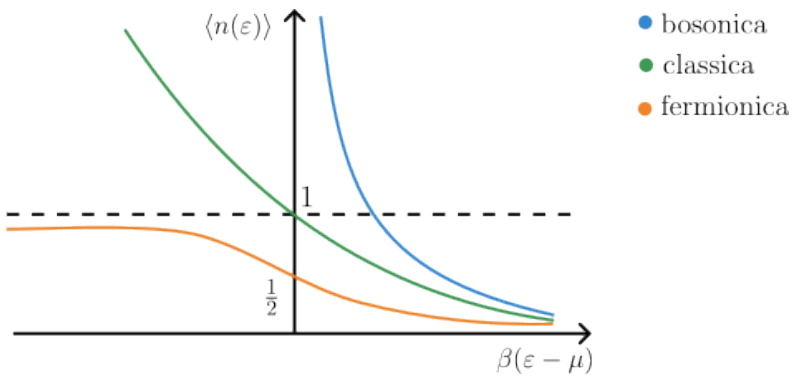
\includegraphics[width=0.6\linewidth]{Immagini/confronto statistiche.png}
    \caption{confronto tra le tre statistiche bosonica, fermionca e classica.}
    \label{fig: confronto statistiche}
\end{figure}

\subsubsection{Temperatura di Fermi}
Consistentemente al principio di esclusione, in ogni microstato fermionico si deve avere che $0 \le \vmedio{n(\epsilon)}_F \le 1$. Nel limite di bassa temperatura, $T \to 0$ e di conseguenza $\beta \to \infty$, per cui
\begin{equation}
    e^{\beta(\epsilon - \mu)} \simeq
    \begin{cases}
        0,\, \epsilon < \mu|_{T=0} \equiv \epsilon_F \\
        \infty,\, \epsilon > \epsilon_F
    \end{cases},
\end{equation}
dove il potenziale chimico del sistema $\epsilon_F$ a temperatura $T = 0$ prende il nome di `ènergia di Fermi'. Dall'espressione della statistica fermionica \eqref{eq: statistica Fermi-Dirac}, in questo limite si ha che
\begin{equation}
    \vmedio{n(\epsilon)}_F \simeq \Theta(\epsilon_ F - \epsilon).
\end{equation}
All'energia di fermi $\epsilon_F$ si può associare la ``temperatura di Fermi'' caratteristica del sistema come
\begin{equation}
    kT_F = \epsilon_F,
\end{equation}
la quale permette di intuire una scala di temperatura ed indicare i limiti di alta e bassa temperatura per un particolare sistema tramite la scala di energia. In altre parole, quando si parla di limite di bassa ed alta temperatura, si prende come punto di riferimento la temperatura $T_F$. Infatti, l'energia di Fermi risulta essere un parametro fondamentale per descrivere il comportamento di un sistema fermionico nel limite di bassa temperatura $T \ll T_F$. 

\subsubsection{Condensazione di Bose - Einstein}
Come detto, per ogni livello $\epsilon$ di un sistema bosonico si deve avere $\mu < \epsilon$; infatti, se così non fosse si avrebbe $\vmedio{n(\epsilon)}_B < 0$, ossia un risultato fisicamente privo di senso in quanto i numeri di occupazione assumono sempre valori maggiori o pari a zero. Quindi, dato che tale condizione sul potenziale chimico vale per ogni $\epsilon$, deve anche valere per il livello fondamentale $\epsilon_0$, per cui $\mu < \epsilon_0$ da cui, nel limite $\mu \to \epsilon_0^-$, segue che
\begin{equation}
\label{eq: condensazione Bose-Einstein}
    \lim_{\mu \to \epsilon_0^-}\vmedio{n(\epsilon)}_B = \infty.
\end{equation}
Normalmente, il numero di particelle che occupano i livelli è irrilevante rispetto ad infinito, tuttavia nel limite termodinamico il numero dei componenti tende proprio ad infinito; quindi una frazione macroscopica di componenti condensa nello stato fondamentale. Questo fenomeno prende il nome di ``condensazione di Bose - Einstein'' ed è prettamente di natura quantistica, ovvero non ha un analogo classico.

\section{Gas di fermioni liberi}
Si consideri un gas di particelle fermioniche libere occupanti un volume $V$ coincidente, per semplicità e senza perdere di generalità, con un cubo di lato $L$, assumendo inoltre che le condizioni al contorno delle funzioni d'onda siano periodiche. In tal caso, gli autostati dell'energia sono associati ai numeri quantici $\vn \in \Z^3$ e la loro energia è
\begin{equation}
    \epsilon(\vn) = \frac{\hbar^2}{2m}\bigg(\frac{2\pi}{L}\bigg)^2|\vn|^2 = \frac{\hbar^2}{2m}|\vk|^2.
\end{equation}
Se le particelle sono dotate di uno spin $s$, allora ogni autostato ha una degenerazione aggiuntiva $g_s = 2s + 1$, dovuta ai possibili autovalori $-\hbar s,\hbar(s - 1),\dots,\hbar(s - 1),\hbar s$ della terza componente di spin. Quindi, l'espressione del potenziale grancanonico è
\begin{equation}
\label{eq: potenziale gas di fermioni (grancanonico)}
    \varpi_F = -\frac{g_s}{\beta}\sum_{\vn\in\Z^3}\log{(1 + ze^{-\beta\epsilon(\vn)})}.
\end{equation}
Per calcolarlo, si deve seguire un certo procedimento. Prima di tutto, ci si concentra sul trovare l'espressione di $\varpi_F$ nel limite termodinamico, quindi si passa dal discreto al continuo con
\begin{equation}
\label{eq: passaggio al continuo gas di fermioni liberi}
    \sum_{\vn\in\Z^3}f(|\vn|) \longrightarrow \frac{V}{2\pi^2}\int_0^\infty dk\,k^2f(|\vk|).
\end{equation}
In questo caso, è più conveniente usare l'energia $\epsilon$ invece del modulo $|\vk| \equiv k$, perciò si opera il cambio di variabili
\begin{equation}
    \epsilon = \frac{\hbar^2}{2m}k^2\quad\Longrightarrow\quad dk = \frac{\sqrt{\pi}}{\lambda_T}\frac{\beta^{1/2}}{\epsilon^{{1/2}}}d\epsilon
\end{equation}
ottenendo
\begin{equation}
    \sum_{\vn\in\Z^3}f(|\vn|) \longrightarrow \frac{V}{V_T}\frac{2}{\sqrt{\pi}}\beta^{3/2}\int_0^\infty d\epsilon\,\epsilon^{1/2}f(\epsilon).
\end{equation}
Il potenziale grancanonico quindi diventa
\begin{equation}
    \begin{split}
        \varpi_F &= -\frac{g_s}{\beta}\frac{V}{V_T}\frac{2}{\sqrt{\pi}}\beta^{3/2}\int_0^\infty d\epsilon\,\epsilon^{1/2}\log(1 + ze^{-\beta\epsilon}) \\
        &= -\frac{g_s}{\beta}\frac{V}{V_T}\frac{2}{\sqrt{\pi}}\int_0^\infty dx\,x^{1/2}\log{(1 + ze^{-x})}
    \end{split},
\end{equation}
dove si è operato il cambio di variabili $x = \beta\epsilon$. L'integrale in questione può essere risolto in una forma standard integrando per parti ottenendo
\begin{equation}
    \frac{2}{\sqrt{\pi}}\int_0^\infty dx\,x^{1/2}\log{(1 + ze^{-x})} = \frac{1}{\Gamma(5/2)}\int_0^\infty dx\,\frac{x^{3/2}}{e^xz^{-1} + 1} \equiv f_{5/2}
\end{equation}
e di conseguenza
\begin{equation}
    \varpi_F = -\frac{g_s}{\beta}\frac{V}{V_T}f_{5/2}(z),
\end{equation}
dove si nota l'introduzione delle funzioni fermioniche $f_\nu(z)$ come
\begin{equation}
\label{eq: funzioni fermioniche}
    f_\nu(z) = \frac{1}{\Gamma(\nu)}\int_0^\infty dx\,\frac{x^{\nu - 1}}{e^xz^{-1} + 1}.
\end{equation}
\begin{obs}
    Le funzioni fermioniche definite nella \eqref{eq: funzioni fermioniche} godono della proprietà di ricorrenza 
    \begin{equation}
        z\frac{\p f_\nu}{\p z} = f_{\nu -1}.
    \end{equation}
    Questa può essere dimostrata partendo da 
    \begin{equation}
        z\frac{\p f}{\p z} = \frac{1}{\Gamma(\nu)}\int_0^\infty dx\,x^{\nu -1}z\frac{\p}{\p z}\bigg(\frac{1}{e^xz^{-1} + 1}\bigg)
    \end{equation}
    e notando che per qualsiasi funzione $F$ si ha
    \begin{equation}
        z\frac{\p}{\p z}F(e^xz^{-1}) = -\frac{\p}{\p x}F(e^xz^{-1});
    \end{equation}
    pertanto, integrando per parti si ha, si ha
    \begin{equation}
        \begin{split}
            z\frac{\p f}{\p z} = -\frac{1}{\Gamma(\nu)}\int_0^\infty dx\,x^{\nu -1}\frac{\p}{\p x}\bigg(\frac{1}{e^xz^{-1} + 1}\bigg) &= \frac{\nu - 1}{\Gamma(\nu)}\int_0^\infty dx\,\frac{x^{\nu - 2}}{e^xz^{-1} + 1} \\
            &= \frac{1}{\Gamma(\nu - 1)}\int_0^\infty dx\, \frac{x^{(\nu - 1) - 1}}{e^xz^{-1} + 1} \\
            &\equiv f_{\nu - 1}(z).
        \end{split} 
    \end{equation}
    Inoltre, sono funzioni perfettamente regolari, monotone crescenti e che si annullano, per definizione, in $z = 0$ per ogni valore di $\nu$.
\end{obs}
Noto il potenziale $\varpi_F$ è adesso possibile derivare la termodinamica del sistema. La pressione $p$ e la densità $1/v$ sono date da
\begin{align}
\label{eq: pressione e densità gas fermioni liberi (grancanonico)}
    p &= -\frac{\varpi_F}{V} = g_s\frac{kT}{V_T}f_{5/2}(z), \\
    \frac{1}{v} &= \frac{\vmedio{N}_F}{V} = -\frac{\beta}{V}z\frac{\p\varpi_F}{\p z}\bigg|_{T,V} = \frac{g_s}{V_T}\frac{\p f_{5/2}(z)}{\p z} = \frac{g_s}{V_T}f_{3/2}(z).
\end{align}
Invece, l'energia interna è data da
\begin{equation}
    \begin{split}
        \vmedio{E} = \frac{\p}{\p\beta}(\beta\varpi_F)\bigg|_{V,z} &= -g_s\frac{\p}{\p\beta}\bigg(\frac{V}{V_T}f_{5/2}(z)\bigg) \\
        &= -g_sVf_{5/2}(z)\frac{\p}{\p\beta}\bigg(\frac{1}{V_T}\bigg) \\
        &= \frac{3}{2}Vg_s\frac{kT}{V_T}f_{5/2}(z) \\
        &=\frac{3}{2}pV,
    \end{split}
\end{equation}
dove si usato il fatto che
\begin{equation}
    \frac{1}{V_T} = \frac{1}{\lambda_T^3} \propto \beta^{-3/2}\quad\Longrightarrow\quad \frac{\p}{\p\beta}\bigg(\frac{1}{V_T}\bigg) = -\frac{3}{2}\frac{1}{\beta V_T}.
\end{equation}
Può essere utile, in particolare per il confronto con i dati sperimentali, considerare come variabile di controllo la densità $1/v$ invece che il potenziale chimico o la fugacità. Infatti, nel caso di un gas nella pratica è molto più semplice controllare la sua densità che gli altri due parametri. Questo tuttavia implica tornare all'ensemble canonico, dove appunto l'insieme delle variabili di controllo sono $\{T,V,1/v\}$ o, equivalentemente, $\{T,V,N\}$. Questo cambio di insieme di variabili può essere effettuato semplicemente invertendo la rispettiva equazione in \eqref{eq: pressione e densità gas fermioni liberi (grancanonico)} e definendo il parametro $\xi$ di proporzionalità alla densità come
\begin{equation}
\label{eq: parametro fermionico}
    \xi = \frac{V_T}{g_sv};
\end{equation}
questo parametro rappresenta il numero di componenti medio in un volume termico $V_T = \lambda_T^3$ e lega il limite classico per cui $z \to 0$ al limite di bassa densità o di alta temperatura dove $\xi \to 0$ tramite la relazione
\begin{equation}
    \xi = f_{3/2}(z).
\end{equation}
Dato che le funzioni fermioniche sono monotone, quest'ultima relazione può essere invertita in termini della fugacità per qualsiasi limite ottenendo
\begin{equation}
    z(\xi) = f_{3/2}^{-1}(\xi).
\end{equation}
Quindi adesso per esprimere le grandezze termodinamiche in funzione di $\xi$ si deve operare la sostituzione $z \to f^{-1}_\nu(\xi)$, in questo modo le espressioni della pressione $p$, della densità $1/v$ e dell'energia interna $\vmedio{E}$ diventano
\begin{align}
    p &= \frac{kT}{v\xi}f_{5/2}(f_{3/2}^{-1}(\xi)), \\ 
    \frac{1}{v} &= \frac{g_s}{V_T}f_{3/2}(f_{3/2}^{-1}(\xi)), \\
    E &= \frac{3}{2}NkT\frac{1}{\xi}f_{5/2}(f_{3/2}^{-1}(\xi)).
\end{align}
Anche se queste relazioni sono valide per ogni valore di $\xi$, ci si concentra sulla loro espansione nei due regimi di alta e bassa temperatura. Inoltre, l'equazione di stato meccanica è
\begin{equation}
\label{eq: equazione di stato meccanica gas fermioni liberi}
    pV = \vmedio{N}kT\frac{1}{\xi}f_{5/2}(f_{3/2}^{-1}(\xi)).
\end{equation}

\setcounter{caso}{0}
\begin{caso}[alta temperatura]
    Le funzioni fermioniche per definizione, data da \eqref{eq: funzioni fermioniche}, ammettono per $z \to 0$ la seguente espansione in serie\footnote{L'espansione si ottiene dalla con un'espansione geometrica dell'integrando 
    \begin{equation}
        \begin{split}
            f_\nu(z) = \frac{1}{\Gamma(\nu)}\int_0^\infty dx\,x^{\nu -1} \frac{ze^{-x}}{1 + ze^{-x}} &= \frac{1}{\Gamma(\nu)}\int_0^\infty dx\,x^{\nu -1}ze^{-x}\sum_{n=0}^\infty(-ze^{-x})^n \\
            &= \frac{1}{\Gamma(\nu)}\sum_{l=1}^\infty(-1)^{l-1}z^l\int_0^\infty dx\,x^{\nu-1}e^{-lx} \\
            &\overset{w = lx}{=} \cancel{\frac{1}{\Gamma(\nu)} }\sum_{l=1}^\infty(-1)^{l-1}\frac{z^l}{l^\nu}\cancel{\int_0^\infty dw\,w^{\nu - 2}e^{-w}}.
        \end{split}
    \end{equation}
    }
    \begin{equation}
    \label{eq: espansione f alta T}
        f_\nu(z) = \sum_{l = 1}^\infty(-1)^{l-1}\frac{z^l}{l^\nu} = z - \frac{z^2}{2^\nu} + \frac{z^3}{3^\nu} + \cdots.
    \end{equation}
    Quindi, sapendo che $z \to 0$ implica $\xi \to 0$ l'espansione in serie della funzione inversa deve essere
    \begin{equation}
    \label{eq: espazione z alta T}
        z(\xi) = f_\nu^{-1}(\xi) = \alpha_1 \xi + \alpha_2\xi^2 + \alpha_3 \xi^3 + \cdots,
    \end{equation}
    per cui se si applica la \eqref{eq: espazione z alta T} nella \eqref{eq: espansione f alta T}, nel caso in cui $\nu = 3/2$, si ha
    \begin{equation}
        \alpha_1 \xi + \alpha_2\xi^2  + \cdots - \frac{1}{2^\nu}(\alpha_1\xi + \alpha_2\xi^2 + \cdots)^2 + \frac{1}{3^\nu}(\alpha_1\xi + \alpha_2\xi^2 + \cdots)^3 + \cdots = \xi.
    \end{equation}
    Uguagliando adesso i coefficienti dello stesso grado in $\xi$ si ottengono i valori dei coefficienti $\alpha_i$
    \begin{align}
        \alpha_1\xi = \xi\quad&\Longrightarrow\quad \alpha_1 = 1, \\
        \alpha_2\xi^2 - \frac{\alpha_1^2\xi^2}{2^\nu} = 0\quad&\Longrightarrow\quad \alpha_2 = \frac{1}{2^\nu}, \\
        \alpha_3 - \frac{2}{(2^\nu)^2} + \frac{1}{3^\nu} = 0\quad&\Longrightarrow\quad \alpha_3 = \frac{1}{2^{\nu-1}} - \frac{1}{3^\nu}\dots
    \end{align}
    Quindi, sostituendo i coefficienti $\alpha_i$ nella \eqref{eq: espazione z alta T}, si ha
    \begin{equation}
        z(\xi) = f_{3/2}^{-1}(\xi) = \xi + \frac{\xi^2}{2^{3/2}} + \bigg(\frac{1}{4} - \frac{1}{3^{3/2}}\bigg)\xi^3 + \cdots
    \end{equation}
    e, di conseguenza, l'equazione di stato \eqref{eq: equazione di stato meccanica gas fermioni liberi} diventa
    \begin{equation}
    \label{eq: equazione di stato meccanica gas fermioni liberi (espansione in serie)}
        \begin{split}
            pV = \vmedio{N}kT\frac{1}{\xi}\sum_{l=1}^\infty(-1)^{l-1}\frac{z^l}{l^{5/2}} &= \vmedio{N}kT\frac{1}{\xi}\bigg[\xi + \xi^2 \bigg(\frac{1}{2^{3/2}} - \frac{1}{2^{5/2}}\bigg) + \cdots\bigg] \\
            &= NkT\bigg(1+ \frac{\xi}{2^{5/2}} + \cdots\bigg).
        \end{split}
    \end{equation}
    Dunque, l'introduzione della statistica fermionica ha causato una correzione nell'equazione di stato meccanica classica, in particolare alla densità, le quali sono analoghe a quelle ottenute per i gas interagenti aventi un potenziale di interazione a corto raggio. La serie in cui si presenta l'equazione \eqref{eq: equazione di stato meccanica gas fermioni liberi (espansione in serie)} è ben nota e prende il nome di ``espansione viriale'', in generale si può esprimere in una forma più compatta introducendo i coefficienti di espansione viriale $b_i$ così da avere
    \begin{equation}
        pV = \vmedio{N}kT\sum_{l=1}^\infty b_l\xi^{l-1}.
    \end{equation}
\end{caso}

\begin{caso}[bassa temperatura]
    Se il limite $z \to 0$ corrisponde al limite classico, il limite $z \to \infty$ corrisponde a quello quantistico. Chiaramente, per definizione $z \to \infty$ implica $\xi \to \infty$, quindi si deve ora studiare l'espansione asintotica delle funzioni fermioniche $f_\nu(z)$. Per farlo, si riscrive la forma generica delle $f_\nu(z)$ come
    \begin{equation}
        f_\nu(z) = \frac{1}{\Gamma(\nu)}\int_0^\infty dx\,\frac{x^{\nu - 1}}{e^{x - \xi} + 1},\quad z = e^\xi.
    \end{equation}
    A questo punto è conveniente spezzare l'integrale sui due intervalli $[0,\xi]$ e $[\xi,\infty)$, in modo da avere
    \begin{equation}
        \begin{split}
            f_\nu(z) &= \frac{1}{\Gamma(\nu)} \bigg( \int_{0}^{\xi}dx\, \frac{x^{\nu-1}}{e^{x-\xi}+1} + \int_{\xi}^{\infty}dx\, \frac{x^{\nu-1}}{e^{x-\xi}+1} \bigg) \\
            &= \frac{1}{\Gamma(\nu)} \bigg( \int_{0}^{\xi}dx\,x^{\nu-1}\frac{e^{\xi-x}}{1+e^{\xi-x}} + \int_{\xi}^{\infty}dx\, \frac{x^{\nu-1}}{e^{x-\xi}+1} \bigg) \\ 
            &= \frac{1}{\Gamma(\nu)} \bigg( \frac{\xi^{\nu}}{\nu} - \int_{0}^{\xi}dx\,  \frac{x^{\nu-1}}{e^{\xi-x}+1} + \int_{\xi}^{\infty}dx\,  \frac{x^{\nu-1}}{e^{x-\xi}+1}\bigg),
        \end{split}
    \end{equation}
    dove, per il primo integrale, nel secondo passaggio si è moltiplicato per $e^{x-\xi}$, nel terzo passaggio si è raccolto $x^{\nu-1}$ e nell'ultimo passaggio si è svolto il primo termine $\int_0^\xi dx\,x^{\nu - 1} = \xi^\nu/\nu$. Ci si aspetta che dopo il primo termine dominante appaiano delle correzioni sempre più trascurabili per $\xi \to \infty$. Ora si opera un cambio di variabili $\eta = \xi - x$ nel primo integrale, mentre nel secondo si pone $\eta = x - \xi$, ottenendo
    \begin{equation}
        \begin{split}
            f_\nu(z) &= \frac{1}{\Gamma(\nu)} \bigg( \frac{\xi^{\nu}}{\nu} - \int_{\xi}^{0}d\eta\,  (-1)\frac{(\xi - \eta)^{\nu-1}}{e^\eta+1} + \int_{\xi}^{\infty}d\eta\,  \frac{(\xi + \eta)^{\nu-1}}{e^{\eta}+1}\bigg) \\
            &= \frac{1}{\Gamma(\nu)} \bigg( \frac{\xi^{\nu}}{\nu} - \int_{0}^{\xi}d\eta\, \frac{(\xi - \eta)^{\nu-1}}{e^\eta+1} + \int_{\xi}^{\infty}d\eta\,  \frac{(\xi + \eta)^{\nu-1}}{e^{\eta}+1}\bigg).
        \end{split} 
    \end{equation}
    Se $\xi \ge 1$, allora $(e^\eta + 1)^{-1} \to 0$ e i contributi di ordine maggiore in $\xi$ sono sempre più trascurabili, quindi integrare su $[0,\xi]$ o su $[0,\infty)$ è indifferente. Con questa considerazione si può quindi scrivere
    \begin{equation}
        \begin{split}
            f_\nu(z) &\simeq \frac{1}{\Gamma(\nu)} \bigg( \frac{\xi^{\nu}}{\nu} - \int_{0}^{\infty}d\eta\, \frac{(\xi - \eta)^{\nu-1}}{e^\eta+1} + \int_{\xi}^{\infty}d\eta\,  \frac{(\xi + \eta)^{\nu-1}}{e^{\eta}+1}\bigg) \\
            &= \frac{1}{\Gamma(\nu)} \bigg\{ \frac{\xi^{\nu}}{\nu} + \int_{0}^{\infty}\frac{d\eta}{e^\eta+1}\bigg[ (\xi + \eta)^{\nu-1} - (\xi - \eta)^{\nu-1} \bigg]\bigg\} \\
            &= \frac{1}{\Gamma(\nu)} \bigg\{ \frac{\xi^{\nu}}{\nu} + \int_{0}^{\infty}\frac{d\eta}{e^\eta+1}\bigg[\sum_{k=0}^\infty\binom{\nu - 1}{k}\eta^k\xi^{\nu - 1 -k} \\
            &- \sum_{k=0}^\infty\binom{\nu-1}{k}(-1)^k\eta^k\xi^{\nu - 1 - k} \bigg]\bigg\} \\
            &= \frac{1}{\Gamma(\nu)} \bigg(\frac{\xi^\nu}{\nu} + \int_0^\infty\frac{d\eta}{e^\eta  + 1}2\sum_{k_{odd}}\binom{\nu - 1}{k}\eta^k\xi^{\nu - 1 -k}\bigg),
        \end{split}
    \end{equation}
    dove nel secondo passaggio si è usata l'espansione binomiale\footnote{La forma generale dell'espansione binomiale è $(a + b)^n = \nsum_{k=0}^n\binom{n}{k}a^{n-k}b^k$.} e nel terzo  si è scritto tutto con un'unica somma sui valori dispari di $k$ dato che il termine $(-1)^k$ comporta la cancellazione dei termini pari e la somma di quelli dispari, da qui anche il fattore due davanti a tale somma. Ora l'obiettivo è quello di calcolare l'integrale su $\eta$ che compare nell'espressione di $f_\nu(z)$, quindi
    \begin{equation}
        \begin{split}
            I_k \equiv \int_0^\infty\frac{d\eta}{e^\eta  + 1}\eta^k = \int_0^\infty d\eta\,\eta^k\frac{e^{-\eta}}{1 + e^{-\eta}} &= \int_0^\infty d\eta\,\eta^ke^{-\eta}\sum_{p=0}^\infty (-1)^pe^{-p\eta} \\
            &= \sum_{q=1}^\infty (-1)^{q-1}\int_0^\infty d\eta\,\eta^ke^{-q\eta} \\
            &\overset{t = q\eta}{=}\sum_{q=1}^\infty \frac{(-1)^{q-1}}{q^{k+1}} \int_0^\infty dt\,t^ke^{-t} \\
            &= \Gamma(k+1)\sum_{q=1}^\infty \frac{(-1)^{q-1}}{q^{k+1}}.
        \end{split}
    \end{equation}
    La somma sull'indice $q$ in $I_k$ può essere ulteriormente divisa nelle due somme sui valori pari e dispari di $q$ così da ottenere
    \begin{equation}
        \begin{split}
            I_k &= \Gamma(k+1)\bigg(\sum_{q_{odd}}\frac{1}{q^{k+1}} - \sum_{q_{even}}\frac{1}{q^{k+1}}\bigg) \\
            &= \Gamma(k +1)[\xi_{odd}(k+1) - \xi_{even}(k+1)].
        \end{split}
    \end{equation}
    Adesso si nota che se si avesse $\xi_{odd}(k+1) + \xi_{even}(k+1)$ questa somma corrisponderebbe alla Zeta di Riemann $\zeta$. Tuttavia, in questo caso si ha una differenza, per cui ci si chiede come si possa ricondurre questa alla Zeta di Riemann. Prima di tutto, si ricorda che esiste una relazione tra le $\xi$ e la $\zeta$ date da
    \begin{align}
        \xi_{even}(k+1) &\overset{q = 2n}{=} \sum_{n = 1}^\infty\frac{1}{(2n)^{k+1}} = \frac{1}{2^{k+1}}\sum_{n=1}^\infty\frac{1}{n^{k+1}} = \frac{1}{2^{k+1}}\zeta(k+1), \\
        \xi_{odd}(k+1) &= \zeta(k+1) - \xi_{even}(k+1) = \bigg(1 - \frac{1}{2^{k+1}}\bigg)\zeta(k+1).
    \end{align}
    Quindi, immediatamente si ha che
    \begin{equation}
        \begin{split}
            \xi_{odd}(k+1) - \xi_{even}(k+1) &= \bigg(1 - \frac{1}{2^{k+1}}\bigg)\zeta(k+1) - \frac{1}{2^{k+1}}\zeta(k+1) \\
            &= \zeta(k+1)\bigg(1 - \frac{1}{2^k}\bigg).
        \end{split}
    \end{equation}
    Pertanto, finalmente si trova che l'integrale vale
    \begin{equation}
        I_k = \Gamma(k+1)\zeta(k+1)\bigg(1 - \frac{1}{2^k}\bigg).
    \end{equation}
    Ritornando allora all'espressione di $f_\nu(z)$ sostituendo il risultato appena ottenuto per $I_k$ si arriva a 
    \begin{equation}
        \begin{split}
            f_\nu(z) & \simeq \frac{(\ln{z})^\nu}{\Gamma(\nu + 1)}\bigg[1 + 2\nu\sum_{k_{odd}}\binom{\nu-1}{k}\Gamma(k+1)\zeta(k+1)\bigg(1 - \frac{1}{2^k}\bigg)\frac{1}{(\ln{z})^{k+1}}\bigg] \\
            &= \frac{(\ln{z})^\nu}{\Gamma(\nu + 1)}\bigg[1 + \frac{\pi^2}{6}\nu(\nu - 1)(\ln{z})^{-2} + \cdots\bigg].
        \end{split}
    \end{equation}
    Dunque, si è trovata una prima approssimazione delle funzioni $f_\nu(z)$ come 
    \begin{equation}
        f_\nu(z) \simeq \frac{(\ln{z})^\nu}{\Gamma(\nu + 1)}.
    \end{equation}
    Ora, questo risultato si può usare per scrivere $\xi$ in funzione del potenziale chimico $\mu$ ricordando che $z = e^{\beta\mu}$, per cui 
    \begin{equation}
        \xi = f_{3/2}(z) \simeq  \frac{(\beta\mu)^{3/2}}{\Gamma(5/2)}\bigg[1 + \frac{\pi}{8}(\beta\mu)^{-2} + \cdots \bigg].
    \end{equation}
    Al primo ordine, si ottiene il risultato completo per il limite $T \to 0$ dato da
    \begin{equation}
        \Gamma(5/2)\xi  =(\beta\mu|_{T=0})^{3/2} \equiv (\beta\epsilon_F)^{3/2},
    \end{equation}
    l'energia di Fermi così definita tramite il potenziale chimico è direttamente legato alla densità del sistema
    \begin{equation}
        \epsilon_F = \frac{\hbar^2}{2m}\bigg(\frac{3}{4\pi g_sv}\bigg)^{3/2},\quad \xi = \frac{V_T}{g_sv}.
    \end{equation}
    Al secondo ordine invece si ha
    \begin{equation}
        (\beta\epsilon_F)^{3/2} \simeq (\beta\mu)^{3/2}\bigg[1 + \frac{\pi^2}{8}(\beta\mu)^{-2}\bigg]
    \end{equation}
    che, imponendo l'ansatz $\beta\mu = \beta\epsilon_F[1 + \alpha(\beta\epsilon_F)^{-2} + \cdots]$, diventa
    \begin{equation}
        \begin{split}
            (\beta\epsilon_F)^{3/2}  &= (\beta\epsilon_F)^{3/2} [1 + \alpha(\beta\epsilon_F)^{-2} + \cdots]^{3/2} \\
            &\times\bigg\{1 + \frac{\pi^2}{8}(\beta\epsilon_F)^{-2}[1 + \alpha(\beta\epsilon_F)^{-2} + \cdots]^{-2}\bigg\} \\
           1 &\simeq \bigg[1 + \frac{3}{2}\alpha(\beta\epsilon_F)^{-2}\bigg] \bigg[1 + \frac{\pi^2}{8}(\beta\epsilon_F)^{-2}\bigg] \\
           1 &\simeq 1 + \bigg(\frac{3}{2}\alpha + \frac{\pi^2}{8}\bigg)(\beta\epsilon_F)^{-2},
        \end{split}
    \end{equation}
    da cui si trova immediatamente che 
    \begin{equation}
        \alpha = -\frac{\pi^2}{12}.
    \end{equation}
    Dunque, è possibile passare all'ensemble canonico tramite
    \begin{equation}
        \beta\mu = \beta\epsilon_F\bigg[1 - \frac{\pi^2}{12}(\beta\epsilon_F)^{-2} + \cdots\bigg],\quad \beta\epsilon_F = [\Gamma(5/2)\xi]^{2/3}.
    \end{equation}
    Nel limite quantistico, l'equazione di stato meccanica \eqref{eq: equazione di stato meccanica gas fermioni liberi (espansione in serie)} assume adesso la forma
    \begin{equation}
        \begin{split}
            pV &= \vmedio{N} k T \frac{\Gamma(5/2)}{(\beta \epsilon_F)^{3/2}} \frac{(\beta \epsilon_F)^{5/2}}{\Gamma(7/2)} \bigg[ 1 - \frac{\pi^2}{12}(\beta \epsilon_F)^{-2} + \cdots \bigg]^{5/2} \\
            &\times\bigg[ 1 + \frac{5}{8}\pi^2 (\beta \epsilon_F)^{-2}(1+\cdots) \bigg] \\
            &= \frac{2}{5} \vmedio{N} \epsilon_F
            \bigg[ 1 + \frac{5\pi^2}{12}(\beta \epsilon_F)^{-2} + \cdots \bigg] \\ 
            &= \frac{2}{5} \vmedio{N} \epsilon_F \bigg[ 1 + \frac{5\pi^2}{12}\bigg(\frac{T}{T_F}\bigg)^2 + \cdots \bigg],
            \end{split} 
    \end{equation}
    mentre per l'energia interna si ha
    \begin{equation}
        \vmedio{E} = \frac{3}{2} pV = \frac{3}{5} \vmedio{N} \epsilon_F
        \bigg[ 1 + \frac{5\pi^2}{12}\bigg(\frac{T}{T_F}\bigg)^2 + \cdots \bigg].
    \end{equation}
    Anche a $T = 0$ (in cui conta solo il primo termine di queste espansioni), si ha una pressione $p_F$ non nulla, che prende il nome di ``pressione di Fermi''
    \begin{equation}
        p_FV = \frac{2}{5} \vmedio{N} \epsilon_F,
    \end{equation}
    con la quale si può esprimere l'energia media a temperatura nulla
    \begin{equation}
        \vmedio{E}_F = \frac{3}{5} \vmedio{N} \epsilon_F.
    \end{equation}
    Quindi in generale, per un gas di fermioni si trova che a temperatura nulla, la pressione e l'energia non sono anch'esse nulle; ciò è dovuto al fatto che anche per $T = 0$ tutti fermioni non si possono disporre sul livello più basso, per via del principio di esclusione di Pauli. Infatti, come visto a $T = 0$ il numero medio di occupazione $\vmedio{n(\epsilon)}_p$ è una funzione Theta di Heaviside. Tutti i livelli fino all'energia di Fermi devono essere occupati, mentre da lì poi nessun livello deve essere occupato. Quindi anche a temperatura nulla, sono comunque occupati degli stati eccitati. Pertanto, utilizzando la \eqref{eq: passaggio al continuo gas di fermioni liberi} per esprimere la degenerazione dei livelli energetici si ottiene esattamente la relazione precedente
    \begin{equation}
        \vmedio{E} = \frac{g_sV}{V_T}\frac{2}{\sqrt{\pi}}\beta^{3/2}\int_0^\infty d\epsilon\,\epsilon^{1/2}\Theta(\epsilon_F - \epsilon).
    \end{equation}
    Per quanto riguarda la capacità termica, nel limite quantistico si ha 
    \begin{equation}
        c_{V,N} = \frac{\p\vmedio{E}}{\p T}\bigg|_{V,N} = \frac{3}{5}N\epsilon_F\bigg[\frac{5}{12}\pi^2\frac{2T}{T_F^2} + \cdots\bigg],
    \end{equation}
    che tende a zero linearmente in accordo con il teorema di Nernst. In generale, l'andamento della capacità termica è perfettamente regolare, come si vede in figura \ref{fig: andamento cap. termica (gas fermioni liberi)}. 
\end{caso} 
\begin{figure}[h]
    \centering
    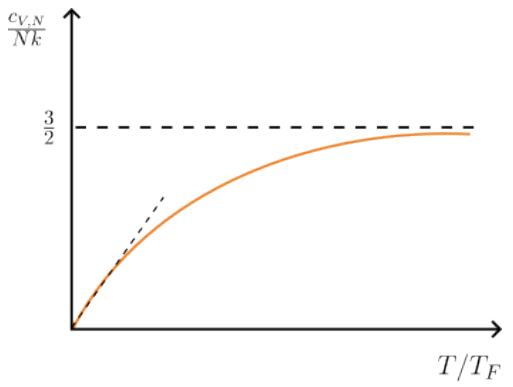
\includegraphics[width=0.5\linewidth]{Immagini/andamento cap. termica (gas fermioni liberi).png}
    \caption{andamento di $c_{V,N}/kN$ in funzione di $T/T_F$ per un gas di fermioni liberi.}
    \label{fig: andamento cap. termica (gas fermioni liberi)}
\end{figure}
\subsection{Elettroni liberi nei metalli}
Nei metalli, gli elettroni di conduzione hanno un'elevata mobilità e la loro termodinamica viene ben riprodotta approssimandoli ad un gas di fermioni liberi di spin $s = 1/2$, cioè $g_s = 2s + 1 = 2$ e quindi con energia di Fermi pari a 
\begin{equation}
    \epsilon_F = \frac{h^2}{2m}\bigg(\frac{3}{8\pi} - \frac{1}{v}\bigg)^{2/3}.
\end{equation}
Si può stimare la densità in funzione del numero di elettroni presenti nel reticolo cristallino come
\begin{equation}
    \frac{1}{v} = \frac{f_ef_a}{a^3},
\end{equation}
dove $f_e$ ed $f_a$ sono rispettivamente il numero di elettroni di conduzione per atomo e quello di atomi per cella del reticolo. Essenzialmente, si contano quanti elettroni di conduzione ci sono per ogni cella e si divide tale numero per il volume della singola cella. Ad esempio, nel caso del sodio l'energia di fermi è
\begin{equation}
    \epsilon_F(\mathrm{Na}) \simeq \SI{5.03e-13}{\joule},
\end{equation}
a cui corrisponde la temperatura di Fermi
\begin{equation}
    T_F(\mathrm{Na}) \simeq \SI{3.64e4}{\kelvin}.
\end{equation}
Dunque, a temperatura ordinaria gli elettroni di conduzione nei metalli formano un gas in un regime profondamente quantistico.

\section{Gas di bosoni liberi}
Per semplicità, si considera un sistema di bosoni aventi spin nullo così che si possa porre $g_s = 0$ semplificando i calcoli; comunque, non è complesso estendere il risultato al caso generale con $g_s = 2s + 1$ dove $s$ è un intero. Ad ogni modo, il procedimento per il gas di bosoni è del tutto analogo a quanto fatto nel caso fermionico. In questo caso, il potenziale grancanonico, invece che \eqref{eq: potenziale gas di fermioni (grancanonico)}, è
\begin{equation}
    \varpi_B = \frac{1}{\beta}\sum_{\vn\in\Z^3}\log{\bigg(1 - ze^{-\beta\epsilon(\vn)}\bigg)}.
\end{equation}
Anche adesso si potrebbe passare dal discreto al continuo tramite un integrale su $\epsilon$ nel limite termodinamico. Tuttavia, facendo l'integrale si sta assegnando ad ogni livello $\epsilon$ una misura nulla, incluso il livello fondamentale $\epsilon_0$. Quest'ultimo però nel caso bosonico assume un ruolo particolare: in questo può condensare una frazione macroscopica di componenti per $\mu \to 0^-$ come discusso nella \eqref{eq: condensazione Bose-Einstein}. Pertanto, non è corretto in generale assegnare misura nulla al contributo di $\epsilon_0$. Si separa quindi quest'ultimo da tutti gli altri associati agli stati eccitati prima di sostituire la somma discreta con l'integrale
\begin{equation}
    \varpi_B = \frac{1}{\beta}\bigg[\log{(1-z)} + \frac{V}{V_T}\frac{2}{\sqrt{\pi}}\beta^{3/2}\int_0^\infty d\epsilon\,\epsilon^{1/2}\log{(1-ze^{-\beta\epsilon})}\bigg].
\end{equation}
Adesso, operando il cambio di variabili $x = \beta\epsilon$ e integrando per parti l'integrale
\begin{equation}
    \frac{2}{\sqrt{\pi}}\int_0^\infty d\epsilon\,(\beta\epsilon)^{1/2}\log{(1-ze^{-\beta\epsilon})} = \frac{-1}{\Gamma(5/2)}\int_0^\infty dx\,\frac{x^{3/2}}{e^xz^{-1} - 1} \equiv -g_{5/2}(z),
\end{equation}
il potenziale $\varpi_B$ diventa
\begin{equation}
    \varpi_B = \frac{1}{\beta}\bigg[\log{(1-z)} - \frac{V}{V_T}g_{5/2}(z)\bigg],
\end{equation}
dove si nota l'introduzione delle funzioni bosoniche $g_\nu(z)$ come
\begin{equation}
    g_\nu(z) = \frac{1}{\Gamma(\nu)}\int_0^\infty dx\,\frac{x^{\nu-1}}{e^xz^{-1} - 1}.
\end{equation}
\begin{obs}
    Anche per le funzioni bosoniche vale una relazione di ricorrenza del tipo
    \begin{equation}
        z\frac{\p g_\nu}{\p z} = g_{\nu - 1}.
    \end{equation}
    Inoltre, sono tutte ben definite, regolari e monotone crescenti, ma solamente nell'intervallo $z \in [0,1]$, a parte la funzione $g_{1/2}(z)$ che risulta asintoticamente divergente ad infinito in $z = 1$ .
\end{obs}
Nelll'intervallo $z\in[0,1]$ le funzioni bosoniche ammettono la rappresentazione in serie 
\begin{equation}
\label{eq: funzioni bosonoiche (espansione in serie)}
    g_\nu(z) = \sum_{l=1}^\infty\frac{z^l}{l^\nu} = z + \frac{z^2}{2^\nu} + \frac{z^3}{3^\nu}+ \cdots,
\end{equation}
in particolare il valore massimo di di queste queste funzioni è 
\begin{equation}
    g_\nu(1) = \sum_{l=1}^\infty\frac{1}{l^\nu} \equiv \zeta(\nu).
\end{equation}
Noto il potenziale, la termodinamica segue come immediatamente
\begin{align}
\label{eq: pressione e densità gas bosoni liberi (grancanonico)}
    p &= -\frac{\varpi_B}{V} = kT\bigg[-\frac{\log{(1-z)}}{V} + \frac{g_{5/2}(z)}{V_T}\bigg], \\
    \frac{1}{v} &= -\frac{\beta z}{V}\frac{\p\varpi_B}{\p z}\bigg|_{T,V} = \frac{1}{V}\bigg[\frac{z}{1-z} + \frac{V}{V_T}g_{3/2}(z)\bigg], 
\end{align}
dove per la densità il primo termine corrisponde al numero medio di particelle nello stato fondamentale $N_0 = z/(1-z)$, mentre il secondo corrisponde al numero medio di particelle in tutti gli stati eccitati $N_e = \vmedio{N} - N_0$. Dalla definizione di $N_0$, si nota che per $z \to 1$ questo diverge ad infinito, ma può crescere al più come $N$ nel limite termodinamico, in quanto non ci possono essere più particelle nello stato fondamentale di quelle totali. Quindi, il primo termine della pressione nella \eqref{eq: pressione e densità gas bosoni liberi (grancanonico)} viene soppresso nel limite termodinamico dato che
\begin{equation}
    -\frac{kT}{V}\log{(1-z)} \simeq \frac{kT}{V}\log{(N_0 + 1)} \le \frac{kT}{V}\log{(N + 1)} \simeq \frac{\log{N}}{N},
\end{equation}
per cui $p$ e $1/v$ nel limite termodinamico diventano
\begin{equation}
    p \simeq \frac{kT}{V_T}g_{5/2}(z),\quad \frac{1}{v} \simeq \frac{1}{V}(N_0 + N_e).
\end{equation}
Invece, per quanto riguarda l'energia interna $\vmedio{E}$, la derivazione nel caso bosonico è identica a quella di quella fermionico e pertanto restituisce 
\begin{equation}
    \vmedio{E} = \frac{3}{2}pV.
\end{equation}
Dunque, essendo le funzioni bosoniche superiormente limitate, a $T$ e $V$ fissati esiste un numero massimo di componenti che possono occupare gli stati eccitati dato da
\begin{equation}
    N_e \le \frac{V}{V_T}\zeta(3/2) \equiv \hatN.
\end{equation}
Assumendo il punto di vista canonico, ossia considerando la densità come variabile indipendente e la fugacità $z$ come dipendente, il sistema assume un comportamento diverso quando $N$ è inferiore o superiore al valore critico $\hatN$. Questa condizione critica può anche essere espressa in termini della densità o, analogamente, del parametro $\eta$ di proporzionalità alla densità come
\begin{equation}
\label{eq: parametro bosonico}
    \eta \equiv \frac{V_T}{v};
\end{equation}
questo parametro è il corrispettivo del parametro $\xi$ definito nella \eqref{eq: parametro fermionico}. Quindi, si passa dal valore critico $\hatN$ a $\hateta$ definito come
\begin{equation}
    \hateta \equiv \zeta(3/2);
\end{equation}
questo parametro critico implica che quando si raggiunge il numero di 2.61 particelle per volume termico a disposizione non è possibile aggiungerne altre, che quindi possono solo occupare lo stato fondamentale. Questa condizione, a $N$ e $V$ fissati, individua la temperatura critica $\hatT$ data da
\begin{equation}
\label{eq: temperatura critica gas di bosoni (grancanonico)}
    \hatT = \frac{h^2}{2\pi mk}[v\zeta(3/2)]^{-2/3},
\end{equation}
dove si è passato dalla relazione
\begin{equation}
    V_{\hatT} = v\zeta(3/2),\quad V_{\hatT} = \lambda_{\hatT}^{3} = \bigg(\frac{h^2}{2\pi mkT}\bigg)^{3/2}.
\end{equation}
A questo punto, è possibile distinguere i soliti due limiti di alta e bassa temperatura, detti rispettivamente regime ``usuale'' e ``di condensazione''. 

\setcounter{caso}{0}
\begin{caso}[alta temperatura]
    Nel regime usuale, ossia nel limite di alta temperatura, il parametro $\eta$ soddisfa la relazione $\eta < \zeta(3/2)$ e consistentemente $z < 1$. Questa condizione si può vedere in due modi:
    \begin{enumerate}
        \item se si tengono fissi $T$ e $V$, allora $\eta < \zeta(3/2)$ implica che $N < \hatN$;
        \item se si tengono fissi $V$ ed $N$, allora $\eta < \zeta(3/2)$ implica che $T > \hatT$.
    \end{enumerate}
    In questo regime, praticamente tutte le particelle sono distribuite nei livelli eccitati secondo la statistica di Bose - Einstein \eqref{eq: statistica Bose-Einstein} per cui
    \begin{equation}
        N \simeq N_e = \frac{V}{V_T}g_{3/2}(z),\quad N_0 = \frac{z}{1 -z} \to 0.
    \end{equation}
    Il passaggio all'ensemble canonico si ottiene invertendo la relazione per $\eta$ in modo da ottenere quella per la fugacità
    \begin{equation}
        z(\eta) = g_{3/2}^{-1}(\eta),
    \end{equation}
    dove la funzione $g_{3/2}(z)$ è perfettamente regolare e monotona crescente su $[0,1]$, quindi può essere invertita numericamente. Tale funzione inversa può essere espressa come una serie di potenze in $\eta$ a partire dalla \eqref{eq: funzioni bosonoiche (espansione in serie)}, il risultato è
    \begin{equation}
        z (\eta)= g_{3/2}^{-1}(\eta) = \eta - \frac{1}{2^{3/2}}\eta^2 + \bigg(\frac{1}{4} - \frac{1}{3^{3/2}}\bigg)\eta^3 + \cdots.
    \end{equation}
    Ricordando le espressioni \eqref{eq: pressione e densità gas bosoni liberi (grancanonico)} si può scrivere l'equazione di stato come un'espansione viriale
    \begin{equation}
        pV = kTN\frac{1}{\eta}g_{5/2}(z) = kTN\frac{1}{\eta}g_{5/2}(g_{3/2}^{-1}(\eta)) = kTN\sum_{l=1}^\infty a_l\eta^{l-1},
    \end{equation}
    il cui membro di destra, nel limite classico in cui $\eta \to 0$, riproduce appunto il risultato classico. Si sono quindi ottenute delle correzioni alla densità analoghe a quella ottenute per il gas di fermioni liberi. Usando questa espressione, l'energia interna diventa
    \begin{equation}
        \vmedio{E} = \frac{3}{2}NkT\sum_{l=1}^\infty a_l\eta^{l-1}.
    \end{equation}
    Nuovamente, per $\eta \to 0$ si ritrova il risultato classico previsto dal teorema di equipartizione dell'energia. Tuttavia, a differenza del caso fermionico, le correzioni viriali sono tutte positive. In questo regime, quindi $c_{V,N}$ cresce come $\eta$ e, a densità fissa, con il diminuire di $T$. Questo appare in contrasto con il teorema di Nernst, in quanto mentre la temperatura scende, la capacità termica aumenta a causa delle correzioni. In realtà al di sotto della temperatura critica $\hatT$ l'espansione smette di essere valida e il comportamento cambia drasticamente, passando al regime di condensazione
\end{caso}
\begin{caso}[bassa temperatura]
    Nel regime di condensazione, ossia nel limite di bassa temperatura, il parametro $\eta$ soddisfa la relazione $\eta > \zeta(3/2)$ e consistentemente $z = 1$. Questa condizione si può vedere in due modi:
    \begin{enumerate}
        \item se si tengono fissi $T$ e $V$, allora $\eta > \zeta(3/2)$ implica che $N > \hatN$;
        \item se si tengono fissi $V$ ed $N$, allora $\eta > \zeta(3/2)$ implica che $T < \hatT$.
    \end{enumerate}
    In questo regime, nei livelli eccitati si trova il massimo numero di particelle permesse 
    \begin{equation}
    \label{eq: frazione bosoni eccitati bassa T (grancanonico)}
        N_e = \frac{V}{V_T}\zeta(3/2) = \frac{N}{\eta}\zeta(3/2).
    \end{equation}
    Quindi, il numero di componenti negli stati eccitati non è più uguale a quella della particelle totali, ma è una sua frazione. Quest'ultima in particolare è data da
    \begin{equation}
        \frac{N_e}{N} = \frac{\hateta}{\eta},
    \end{equation}
    mentre i componenti rimanenti ``condensano'' nello stato fondamentale $N_0 = N - N_e = N[1 - \zeta(3/2)]$, per cui la loro frazione è
    \begin{equation}
         \frac{N_0}{N} = 1 - \frac{\hateta}{\eta}.
    \end{equation}
    Tenendo conto del fatto che nel regime usuale $\eta < \hateta$, si ha
    \begin{equation}
        \frac{N_e}{N} = 1, \quad \eta < \hateta.
    \end{equation}
    L'andamento delle funzioni eccitate e non eccitate è mostrato in figura \ref{fig: andamento di Ne (gas bosoni liberi).}. Da questa si può vedere come per $\eta > \hateta$ cominciano a coesistere due ``fasi'' diverse:
    \begin{enumerate}
        \item la fase normale, dove $N_e/N$ componenti sono distribuite tra i vari livelli eccitati secondo la statistica di Bose - Einstein;
        \item la fase condensata, dove $N_0/N$ sono nello stato fondamentale.
    \end{enumerate}
    \begin{figure}[h]
        \centering
        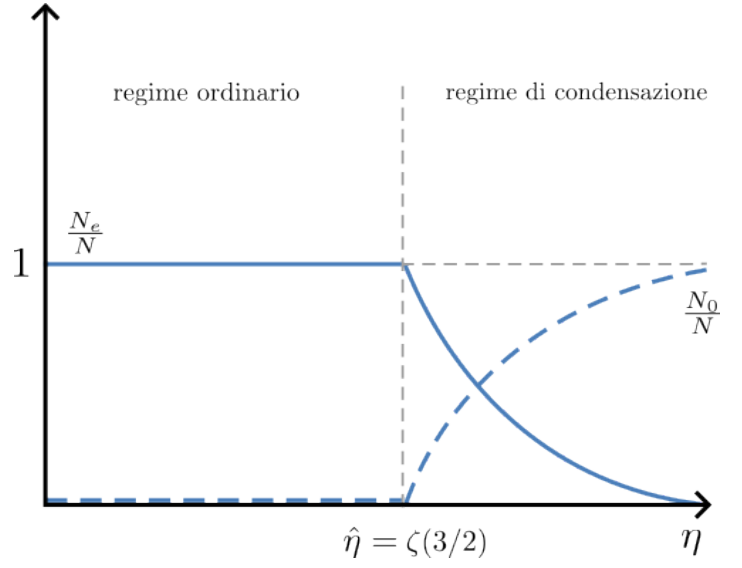
\includegraphics[width=0.5\linewidth]{Immagini/andamento di Ne (gas bosoni liberi).png}
        \caption{andamento di $N_e/N$ in funzione di $\eta$ per un gas di bosoni liberi.}
        \label{fig: andamento di Ne (gas bosoni liberi).}
    \end{figure}
    Anche se coesistono, la fase condensata tende a prevalere su quella normale al crescere di $\eta$, seguendo una transizione omogenea. La fugacità $z$ in questo regime si ottiene invertendo la definizione di $N_0$ ottenendo, considerandola nel limite termodinamico, che
    \begin{equation}
         z = \frac{N_0}{N_0 + 1} \to 1,\quad N_0 \to \infty,
    \end{equation}
    e il conseguente andamento in funzione di $\eta$ mostrato in figura \ref{fig: andamento di z (gas bosoni liberi)}. 
    \begin{figure}[h]
        \centering
        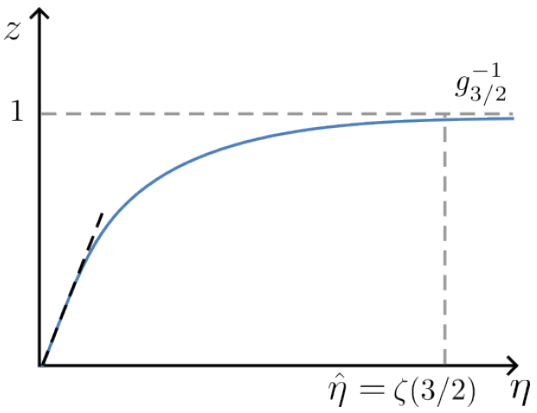
\includegraphics[width=0.45\linewidth]{Immagini/andamento di z (gas bosoni liberi).png}
        \caption{andamento di $z$ in funzione di $\eta$ per un gas di bosoni liberi.}
        \label{fig: andamento di z (gas bosoni liberi)}
    \end{figure}
    Ricordando l'espressione della pressione nella \eqref{eq: pressione e densità gas bosoni liberi (grancanonico)}, in questo regime $p$ si riduce al valore costante
    \begin{equation}
        p \simeq \frac{kT}{V_T}\zeta(5/2),
    \end{equation}
    mentre l'equazione di stato diventa
    \begin{equation}
        pV = kTN\frac{1}{\eta}\zeta(5/2),\quad \eta > \hateta \equiv \zeta(3/2),
    \end{equation}
    la quale al valore critico assume la forma
    \begin{equation}
        pV|_{\eta = \hateta} = kTN_e\frac{\zeta(5/2)}{\zeta(3/2)} \simeq 0.513 \times kTN,
    \end{equation}
    ossia lo stesso valore limite ottenibile nel regime usuale. Dunque, la quantità $pV/NkT$ è continua ovunque compreso nel punto critico $\hateta$, oltre il quale l'andamento segue un'iperbole come mostrato in figura \ref{fig: andamento pV (gas bosoni liberi)}.
    \begin{figure}[h]
        \centering
        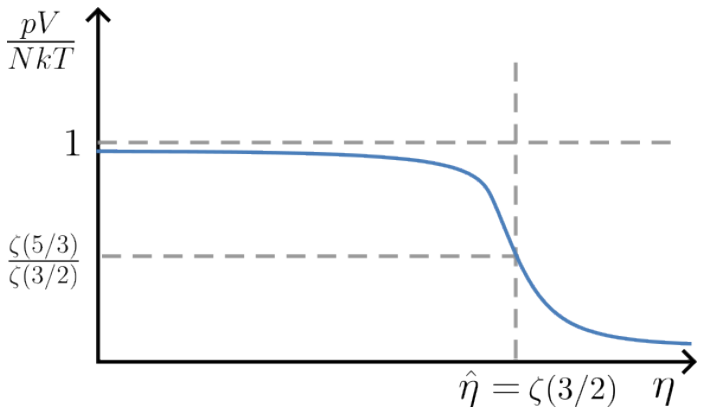
\includegraphics[width=0.5\linewidth]{Immagini/andamento pV (gas bosoni liberi).png}
        \caption{andamento di $pV/NkT$ in funzione di $\eta$ per un gas di bosoni liberi.}
        \label{fig: andamento pV (gas bosoni liberi)}
    \end{figure}
    Questo è anche l'andamento dell'energia interna per $\eta > \hateta$, infatti
    \begin{equation}
        E = \frac{3}{2}pV \simeq \frac{3}{2}kTN\frac{1}{\eta}\zeta(5/2),
    \end{equation}
    la quale può essere riscritta, usando la \eqref{eq: frazione bosoni eccitati bassa T (grancanonico)}, come
    \begin{equation}
        E =  \frac{3}{2}kTN_e\frac{\zeta(5/2)}{\zeta(3/2)}
    \end{equation}
    mostrando così come sia solo la fase `usuale'' a contribuire all'energia interna, dato che nella fase condensata tutte le componenti sono nel livello $\epsilon_0 = 0$: le componenti nello stato fondamentale non contribuiscono alla pressione, quindi quando la frazione di particelle nello stato eccitato diminuisce, diminuisce la pressione. Per quanto riguarda la capacità termica, considerando che $V_T = \lambda_T^3 \propto T^{-3/2}$ e $E\propto T^{5/2}$, questa è
    \begin{equation}
        c_{V,N} = \frac{3}{2}kN\frac{5}{2}\frac{1}{\eta}\zeta(5/2),
    \end{equation}
    la quale valutata nel punto critico diventa
    \begin{equation}
        c_{V,N}|_{\eta = \hateta} = \frac{3}{2}kN\frac{\zeta(5/2)}{\zeta(3/2)} \simeq 1.26\times\frac{3}{2}kN,
    \end{equation}
    che è il medesimo valore ottenibile dall'espansione viriale per $\eta \to \hateta^-$ nel regime usuale. Dunque, la capacità termica è continua rispetto al punto critico $\hateta$; tuttavia, il suo andamento in figura \ref{fig: andamento cap. termica (gas bosoni liberi)} mostra una cuspide proprio in $\hateta$ implicando che la derivata di $c_{V,N}$ è discontinua. 
    \begin{figure}[h]
        \centering
        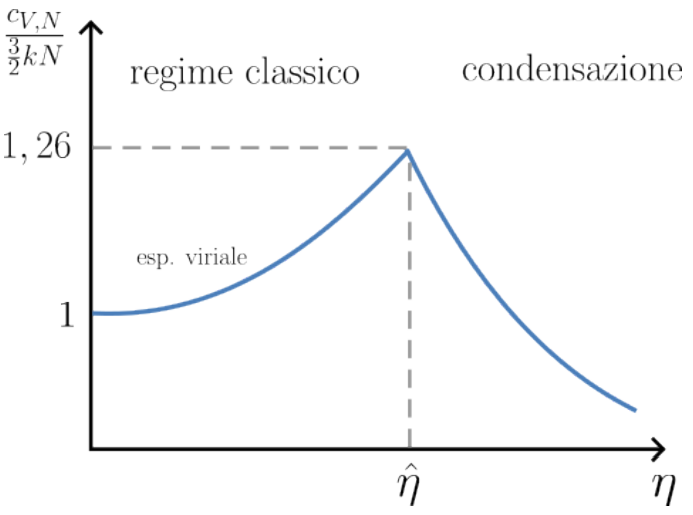
\includegraphics[width=0.45\linewidth]{Immagini/andamento cap. termica (gas bosoni liberi) 1.png}
        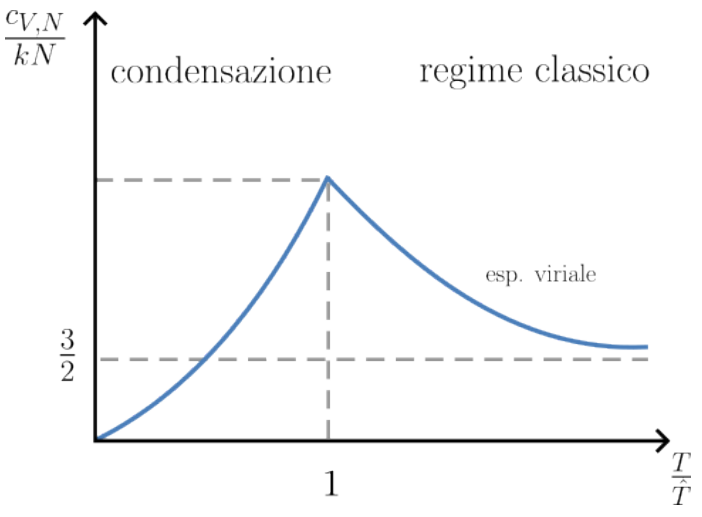
\includegraphics[width=0.45\linewidth]{Immagini/andamento cap. termica (gas bosoni liberi) 2.png}
        \caption{andamento di $3c_{V,N}/2kN$ per un gas di bosoni liberi in funzione di: (i) $\eta$; (ii) $T/\hatT$.}
        \label{fig: andamento cap. termica (gas bosoni liberi)}
    \end{figure}
    Spesso per il confronto con i dati sperimentali, si considera un sistema avente $N$ e $V$ fissati e ci si concentra sulla dipendenza da $T$ delle varie quantità termodinamiche. In particolare, si ha
    \begin{equation}
        \eta = \frac{V_T}{v} = \frac{\lambda_T^3}{v} = cT^{-3/2},\quad c = \frac{1}{v}\bigg(\frac{h^2}{2\pi mk}\bigg)^{3/2}.
    \end{equation}
    Il valore critico $\hateta$ individua la temperatura critica $\hatT$ tramite
    \begin{equation}
        \zeta(3/2) \equiv \hateta = c\hatT^{-3/2}\quad\Longrightarrow\quad c = \zeta(3/2)\hatT^{3/2},
    \end{equation}
    per cui si può scrivere 
    \begin{equation}
        \eta = \bigg(\frac{\hatT}{T}\bigg)^{3/2}\zeta(3/2),
    \end{equation}
    ottenendo il grafico dell'andamento di $c_{V,N}/kN(\hatT/T)$ sempre in figura \ref{fig: andamento cap. termica (gas bosoni liberi)}. Questo andamento è qualitativamente molto simile al grafico del calore specifico dell'$\ce{^4He}$ liquido. Nel 1938 London suggerì che questa singolarità per $T \simeq \SI{2.19}{\kelvin}$ fosse spiegabile in termini della condensazione di Bose - Einstein. In effetti, se si sostituiscono nella i valori appropriati di massa e volume molare dell'$\ce{^4He}$ nella \eqref{eq: temperatura critica gas di bosoni (grancanonico)} si ottiene
    \begin{equation}
        \hatT \simeq \SI{3.13}{\kelvin}.
    \end{equation}
    L'interpretazione di questa transizione dell'elio liquido come condensazione di Bose - Einstein è in accordo con il modello empirico semi-fenomenologico di Tisza basato sul fatto che le caratteristiche di una transizione di questo tipo dovessero corrispondere alla coesistenza di due fasi fluide diverse. Le due fasi sono quelle ``normale'' e quella ``condensata'' che compare per $T = \hatT$ e diviene dominante con il diminuire di $T$.
\end{caso}

\subsection{Gas di fotoni}
Si consideri una cavità di volume $V$ le cui componenti sono mantenute a temperatura costante $T$, al cui interno è intrappolata della radiazione elettromagnetica. Dato che si sta parlando di particelle a massa nulla, la situazione è leggermente diversa da quella dei bosoni liberi studiati precedentemente, quindi non si rientra nella condensazione di Bose - Einstein. Nella prospettiva dell'Elettrodinamica quantistica si ha un gas di quanti del campo elettromagnetico, i fotoni possono essere creati o annichilati nelle interazioni con la materia delle pareti: il loro numero non è fisso e non c'è costo energetico nel variarlo. Dunque, il potenziale
chimico è nullo $\mu = 0$ e per la dualità onda-particella l'energia di ogni singolo fotone è $\epsilon = \hbar\omega$. La conseguente relazione di dispersione è $\omega = c|\vk| \equiv ck$. Inoltre, il fotone possiede due stati di elicità dati da $\pm\hbar$ che corrispondono alle due possibili polarizzazioni trasverse indipendenti dalle onde elettromagnetiche, quindi $g_s = 2$ e la degenerazione dei fotoni con la stessa energia è data da
\begin{equation}
    g(\omega) = \frac{2V}{2\pi^2c^3}\omega^2 = \frac{V}{\pi^2c^3}\omega^2.
\end{equation}
Il potenziale grancanonico $\varpi_B$ per un gas ideale di bosoni liberi, nel caso del gas di fotoni, diventa
\begin{equation}
    \varpi = kT\int_0^\infty d\omega\,g(\omega)\log{(1 - e^{-\beta\hbar\omega})} = \frac{kTV}{\pi^2c^3}\int_0^\infty d\omega\,\omega^2\log{(1 - e^{-\beta\hbar\omega})},
\end{equation}
da cui si possono derivare le quantità termodinamiche di interesse. Partendo dalla pressione, questa è data da
\begin{equation}
    p = -\frac{\varpi}{V} = \frac{kT}{\pi^2c^3}\int_0^\infty d\omega\,\omega^2\log{(1 - e^{-\beta\hbar\omega})},
\end{equation}
che integrata per parti, considerando l'annullamento dei termini al bordo e cambiando variabile con $x = \beta\hbar\omega$, diventa
\begin{equation}
    \begin{split}
        p = -\frac{kT}{\pi^2c^3}\int_0^\infty\frac{d(\omega^3)}{3}\log{(1 - e^{-\beta\hbar\omega})} &= \frac{kT}{3\pi^2c^3}\int_0^\infty d\omega\,\omega^3\frac{\beta\hbar e^{-\beta\hbar\omega}}{1 - e^{-\beta\hbar\omega}} \\
        &\overset{x=\beta\hbar\omega}{=} \frac{k^4T^4}{3\pi^2c^3\hbar^3}\int_0^\infty dx\,\frac{x^3e^{-x}}{1 - e^{-x}}.
    \end{split}
\end{equation}
Adesso ricordando il risultato ottenuto per la costante di Debye in \eqref{eq: costante di Debye}, si ha che la pressione del gas di fotoni è
\begin{equation}
\label{eq: pressione gas di fotoni}
    p = \frac{\pi^2k^4}{45c^3\hbar^3}T^4 = \frac{4}{3c}\sigma T^4,\quad \sigma = \frac{\pi^2k^4}{60c^2\hbar^3} \simeq \SI{5.67}{\joule\meter^{-2}\second^{-1}\kelvin^{-4}},
\end{equation}
dove la costante di proporzionalità $\sigma$ prende il nome di ``costante di Stefan - Boltzmann''. Quindi, l'energia interna è ottenuta come al solito ma considerando che adesso $\mu = 0$, per cui
\begin{equation}
    \begin{split}
        \vmedio{E} = \frac{\p(\beta\varpi)}{\p\beta}\bigg|_{N,\mu = 0} &= \frac{V}{\pi^2c^3}\int_0^\infty d\omega\,\omega^2\frac{\p}{\p\beta}\log{(1 - e^{-\beta\hbar\omega})} \\
        &= \frac{V}{\pi^2c^3}\int_0^\infty d\omega\,\omega^2\hbar\omega\frac{e^{-\beta\hbar\omega}}{1 - e^{-\beta\hbar\omega}},
    \end{split}
\end{equation}
che in termini della pressione può essere espressa come
\begin{equation}
    \vmedio{E} = 3pV.
\end{equation}
Inoltre, si può scrivere la densità di energia totale come
\begin{equation}
    \frac{\vmedio{E}}{V} = \int_0^\infty d\omega\,\rho(\omega),
\end{equation}
dove $\rho(\omega)$ rappresenta la densità di energia per unità di frequenza ed è data dalla legge di Planck della radiazione
\begin{equation}
    \rho(\omega) = \frac{\omega^2}{\pi^2c^3}\frac{\hbar\omega}{e^{\beta\hbar\omega} - 1}.
\end{equation}
Quindi la densità di energia totale all'interno del corpo nero è distribuita in onde di frequenza diversa. Pertanto, ci si può chiedere quale sia la densità di energia presenta all'interno del corpo nero a seconda della frequenza. In realtà, nella pratica non si misura direttamente la densità di energia all'interno del corpo nero, ma si studia la radiazione emessa da esso; in particolare, si può mostrare che il flusso di energia per unità di frequenza e di superficie di un foro nella cavità è dato da
\begin{equation}
    I(\omega) = \frac{c}{4}\rho(\omega).
\end{equation}
Si definisce anche l'``emissività'' $\mathcal{E}$ di un corpo come l'intensità di tale energia emessa per unità di superficie 
\begin{equation}
    \mathcal{E} := \int_0^\infty d\omega\,I(\omega) = \frac{c}{4}\frac{\vmedio{E}}{V} = \sigma T^4,
\end{equation}
permettendo la derivazione sperimentale della costante di Stefan - Boltzmann.

Dato che il numero medio di fotoni può variare, allora è lecito chiedersi quale sia il valore medio del numero di fotoni $\vmedio{N}$. Questo si può calcolare dalla \eqref{eq: numero medio N (grancanonico)}, ponendo $z = 1$ e $\mu = 0$, adattando la definizione al continuo
\begin{equation}
    \vmedio{N} = \frac{V}{\pi^2c^3}\int_0^\infty d\omega\,\omega^2\frac{1}{e^{\beta\hbar\omega} - 1} \equiv V\int_0^\infty d\omega\, u(\omega),
\end{equation}
dove si è definita la densità di fotoni per unità di frequenza come
\begin{equation}
    u(\omega) = \frac{\omega^2}{\pi^2c^3}\frac{1}{e^{\beta\hbar\omega} - 1},
\end{equation}
la quale è direttamente collegata alla densità di energia per unità di frequenza tramite $\rho(\omega) = \hbar\omega u(\omega)$, dato che ogni fotone contribuisce con un quanto di energia $\epsilon = \hbar\omega$. Operando poi il cambio di variabile $x = \beta\hbar\omega$, si ottiene
\begin{equation}
    \frac{\vmedio{N}}{V} = \frac{k^3T^3}{\pi^2c^3\hbar^3}\int_0^\infty dx\,\frac{x^2}{e^x - 1} \equiv \frac{k^3T^3}{\pi^2c^3\hbar^3}J,
\end{equation}
dove l'integrale $J$ può essere valutato in un modo analogo a quanto fatto per calcolare la costante di Debye in \eqref{eq: costante di Debye} tramite l'espansione in serie geometrica ottenendo
\begin{equation}
     J = \Gamma(3)\zeta(3) = 2\zeta(3) \simeq 2.401.
\end{equation}
Dunque, la densità media dei fotoni è
\begin{equation}
\label{eq: densità gas di fotoni}
    \frac{\vmedio{N}}{V} = 2\zeta(3)\frac{k^3T^3}{\pi^2c^3\hbar^3}.
\end{equation}
Sfruttando infine la formula della pressione \eqref{eq: pressione gas di fotoni} in combinazione con la relazione appena trovata per la densità \eqref{eq: densità gas di fotoni} si ottiene l'equazione di stato meccanica nella forma
\begin{equation}
    pV = \frac{\zeta(4)}{\zeta(3)}\vmedio{N}kT \simeq 0.9003\times \vmedio{N}kT.
\end{equation}
Dunque, l'equazione di stato meccanica non corrisponde a quella classica, ma è corretta da un fattore moltiplicativo pari a circa $0.9003$.

\section{Gas classico interagente}
Fino ad ora si sono considerati solamente sistemi non interagenti, in cui l'energia è additiva nei contributi delle varie componenti, e si sono visti emergere effetti di interazione di tipo statistico nei sistemi quantistici che si creano quando le componenti sono indistinguibili. Tuttavia, non si sono mai considerate situazioni con termini di interazione presenti sin dall'inizio nell'hamiltoniana microscopica. In molte situazioni i termini di interazione sono ``piccoli'', come nel caso di un gas nel limite di alta temperatura o, equivalentemente, di bassa densità. In tal caso, si può procedere sistematicamente ad includere il loro effetto tramite una espansione perturbativa. Tale metodo, che storicamente precede quello analogo usato in Teoria dei campi, prende il nome di ``cluster expansion''. Per semplicità, ci si limita al primo ordine perturbativo, considerando un gas classico. 

Quindi, l'hamiltoniana di un sistema interagente ad $N$ componenti identiche di massa $m$ è
\begin{equation}
    H = \sum_{i=1}^N\frac{|\vp_i|^2}{2m} + \sum_{i < j}u_{ij}.
\end{equation}
Al proposito di seguire una trattazione perturbativa, si assume che le interazioni siano molto più ``piccole'' rispetto all'energia termica e che il potenziale di interazione dipenda unicamente dal modulo della distanza tra le componenti
\begin{equation}
    u_{ij} \equiv u(\vq_{ij}) = u(|\vq_i - \vq_j|).
\end{equation}
Se si tratta questo sistema classicamente, la funzione di partizione risulta essere
\begin{equation}
\label{eq: funzione di partizione sistema interagente (canonico)}
    \begin{split}
        Z_{(N)} &= \frac{1}{N!}\int\frac{d^{3N}p\,d^{3N}q}{h^{3N}}\,e^{-\beta H} \\
        &= \frac{1}{N!}\int\frac{d^{3N}p}{h^{3N}}\,e^{-\beta\sum_i|\vp_i|^2/2m}\int d^{3N}q\,e^{-\beta \sum_{i<j}u_{ij}} \\
        &\equiv \frac{1}{N!}\mathcal{P}(N)\mathcal{C}(N),
    \end{split}
\end{equation}
dove $\intp$ e $\intconfig$ sono rispettivamente gli integrali sui momenti e sulle coordinate, detto ``di configurazione''. In particolare, $\intconfig$ si può riscrivere come
\begin{equation}
    \intconfig = \int d^{3N}q\,\prod_{i<j}e^{-\beta u_{ij}},
\end{equation}
da cui si nota che, essendo l'integrando un esponenziale e quindi sempre positivo, allora anche $\intconfig \ge 0$. Chiaramente, nel caso ideale in assenza di interazioni, $u_{ij} = 0$ e quindi $\intconfig = \int d^{3N}q = V^N$. 

Adesso l'obiettivo è trovare un modo per organizzare $\intconfig$; nel caso interagente è conveniente introdurre una quantità che tenda a zero quando $\beta u_{ij}$ è ``piccolo'', consistentemente alle ipotesi assunte per il potenziale di interazione. Si definisce quindi
\begin{equation}
    f_{ij} := e^{-\beta u_{ij}} - 1 : \begin{cases}
        f_{ij} \to 0,\,\beta u_{ij} = 0 \\
        f_{ij} \ll 1,\,\beta u_{ij} \ll 1
    \end{cases}.
\end{equation}
L'espansione perturbativa pertanto non è altro che un'espansione per ``piccoli'' valori di $f$: Nel limite $\beta u_{ij} \ll 1$ è possibile espandere l'integrale di configurazione in potenze di $f$ come
\begin{equation}
    \intconfig = \int d^{3N}q\,\prod_{i<j}(1 + f_{ij}) = \int d^{3N}q\,\bigg(1 + \sum f_{ij} + \sum f_{ij}f_{kl} + \cdots\bigg),
\end{equation}
dove le somme simboliche nell'integrando stanno a rappresentare i termini aventi una copia di $f$, due copie di $f$, e così via. Dal primo termine, non essendoci alcuna dipendenza da $f$, si ritrova il risultato del sistema non interagente; dopo il primo termine, compaiono le correzioni dovute all'interazione, i vari contributi di tale espansione possono venire rappresentati graficamente come
\begin{align}
    \circled{i} &\equiv \int d^3q_i = V, \\
    \circled{i} - \circled{j} &\equiv \int d^3q_i\,d^3q_j\,f_{ij} \\
    \circled{i} - \circled{j} - \circled{k} &\equiv \int d^3q_i\,d^3q_j\,d^3q_k\,f_{ij}f_{jk}.
\end{align}
I grafici connessi prendono il nome di ``clusters'', da qui il nome ``cluster expansion'' del metodo. Limitandosi ai cluster di secondo ordine, ossia al primo ordine non banale, si ha
\begin{equation}
    \begin{split}
        \intconfig &\simeq \int d^{3N}q + \sum_{i<j}\int d^{3(N-2)}q\int d^3q_i\,d^3q_j\,f_{ij} \\
        &= V^N + V^{N-2}\sum_{i<j}\int d^3q_i\,d^3q_j\,f_{ij},
    \end{split}
\end{equation}
che può essere scritto in termini di clusters osservando che le variabili $i$ e $j$ sono mute essendo integrate e quindi restituiscono il medesimo contributo per qualsiasi $f_{ij}$ permettendo di scegliere $i = 1$ e $j = 2$; quindi si ha
\begin{equation}
\label{eq: integrale di configurazione II ordine}
    \begin{split}
        \intconfig &\simeq V^N\bigg[1 + \binom{N}{2}\frac{1}{V^2}\int d^3q_1\,d^3q_2\,f_{12} \bigg] \\
        &= V^N\bigg[1 + \frac{N(N-1)}{2V^2}\circled{i}-\circled{j}\bigg].
    \end{split}
\end{equation}
Sostituendo l'espressione dell'integrale di configurazione \eqref{eq: integrale di configurazione II ordine} in quella della funzione di partizione \eqref{eq: funzione di partizione sistema interagente (canonico)} si ottiene
\begin{equation}
    Z_{(N)} = \frac{1}{N!}\bigg(\frac{V}{V_T}\bigg)^N\bigg[1 + \frac{N(N-1)V_T}{V}b_2 + \cdots\bigg],
\end{equation}
dove si sono definiti i coefficienti $b_i$, la cui forma è determinata unicamente da quella del potenziale di interazione $u_{ij}$; in particolare, per ragioni collegate all'organizzazione dei termini successivi, si pone
\begin{equation}
    b_2 := \frac{1}{2VV_T}\circled{i}-\circled{j}.
\end{equation}

Se si considerano anche le correzioni successive al primo ordine non banale, risulta sempre più conveniente passare all'enesemble grancanonico e definire la funzione di partizione grancanonica
\begin{equation}
    \begin{split}
        Q = \sum_{N=0}^\infty z^NZ_{(N)} &= \sum_{N=0}^\infty z^N\frac{1}{N!}\bigg(\frac{V}{V_T}\bigg)^N\bigg[1 + \frac{N(N-1)V_T}{V}b_2 + \cdots\bigg] \\
        &= \sum_{N=0}^\infty \frac{1}{N!}\bigg(\frac{zV}{V_T}\bigg)^N  + b_2\sum_{N=2}^\infty \frac{z^N}{(N-2)!}\bigg(\frac{V}{V_T}\bigg)^{N-1} + \cdots,
    \end{split}
\end{equation}
che all'ordine considerato coincide\footnote{Infatti, ricordando l'espansione in serie $e^x = \sum_{n=0}^\infty x^n/n!$, si ha
\begin{align}
        \exp{\bigg[\frac{zV}{V_T}(1 + b_2z + \cdots)\bigg]} &= \sum_{N=0}^{\infty} \frac{1}{N!} \bigg(\frac{zV}{V_T}\bigg)^N
        \bigg(1 + b_2 z + \cdots \bigg)^N \\
        &\simeq \sum_{N=0}^{\infty} \frac{1}{N!}
        \bigg(\frac{zV}{V_T}\bigg)^N
        \bigg(1 + N b_2 z + \cdots \bigg) \\
        &= \sum_{N=0}^{\infty} \frac{1}{N!} \bigg(\frac{zV}{V_T}\bigg)^N + b_2 \sum_{N=2}^{\infty}\frac{z^{N+1}}{(N-1)!} \bigg(\frac{V}{V_T}\bigg)^N + \cdots.
\end{align}
Per confrontare le due sommatorie, entrambe devono essere alla potenza $N$,
quindi si pone $M = N + 1$ nel secondo termine, cosicché 
\begin{align}
    \exp{\bigg[\frac{zV}{V_T}(1 + b_2z + \cdots)\bigg]} &= \sum_{N=0}^{\infty} \frac{1}{N!} \bigg(\frac{zV}{V_T}\bigg)^N + b_2 \sum_{M=2}^{\infty} \frac{z^M}{(M-2)!} \bigg(\frac{V}{V_T}\bigg)^{M-1} + \cdots = Q.
\end{align}} con
\begin{equation}
    Q = \exp{\bigg[\frac{zV}{V_T}(1 + b_2z + \cdots)\bigg]}.
\end{equation}
Dalla funzione di partizione si deduce il potenziale grancanonico 
\begin{equation}
    \varpi = -kT\log{Q} = -\frac{zVkT}{V_T}(1 + b_2z + \cdots),
\end{equation}
da cui a sua volta si deducono le quantità termodinamiche
\begin{align}
\label{eq: pressione e N medio gas interagente (grancanonico)}
    p &= -\frac{\varpi}{V} = \frac{zkT}{V_T}(1 + b_2z + \cdots), \\
    \vmedio{N} &= -\beta z\frac{\p\varpi}{\p z}\bigg|_{T,V} = \frac{V}{V_T}(z + 2b_2z^2 + \cdots).
\end{align}
Per ritornare alla trattazione canonica, si può semplicemente scrivere la relazione
\begin{equation}
    \eta \equiv \frac{\vmedio{N}}{V}V_T = z + 2b_2z^2 + \cdots
\end{equation}
che può essere invertita in
\begin{equation}
    z = \eta - 2b_2\eta^2 + \cdots,
\end{equation}
la quale sostituita nelle \eqref{eq: pressione e N medio gas interagente (grancanonico)} permette di scrivere l'equazione di stato come
\begin{equation}
    pV = kT\vmedio{N}(1 - b_2\eta + \cdots).
\end{equation}
In generale, considerando correzioni di ordine più alto, si ottiene l'espansione viriale
\begin{equation}
\label{eq: equazione di stato (espansione viriale)}
    pV = kT\vmedio{N}\sum_{l=1}^\infty a_l\eta^{l-1},
\end{equation}
dove gli $a_i$ sono i coefficienti viriali.
\begin{obs}
    Si può mostrare che il coefficiente $a_l$ è determinato dai clusters fino all'ordine $l$; per cui, se si decide di fermarsi ad un'ordine $l$ nella sommatoria, allora si considerano i cluster solo fino a quell'ordine.
\end{obs}
Dunque, si è trovato che l'effetto dell'interazione è quello di diminuire $pV$, perché tendono a formare stati legati e fare meno pressione. 

\subsection{Secondo coefficiente viriale}
L'obiettivo è calcolare il secondo coefficiente viriale $a_2$ dell'espansione \eqref{eq: equazione di stato (espansione viriale)} per un potenziale il cui andamento è mostrato in figura \ref{fig: potenziale coefficiente a2}. Un'espressione semi-empirica per potenziali di questo tipo è data dal potenziale di Lennard - Jones
\begin{equation}
\label{eq: potenziale Lennard-Jones}
    u(r_{ij}) = 4\epsilon\bigg[\bigg(\frac{\sigma}{r_{ij}}\bigg)^{12} - \bigg(\frac{\sigma}{r_{ij}}\bigg)^{6}\bigg],
\end{equation}
dove $\epsilon$ è l'energia associata al minimo del potenziale in $r_0 = 2^{1/6}\sigma$. In realtà, l'approssimazione che si usa qui è ancora più limitata, continuando però ad essere adatta all'ambito statistico. L'idea, mostrata in figura \ref{fig: potenziale coefficiente a2}, è quella di rimpiazzare la parte repulsiva del potenziale con un ``muro'' repulsivo
\begin{equation}
\label{eq: potenziale Lennard-Jones approx.}
    u(r_{ij}) = 
    \begin{cases}
        \infty,\, r < r_0\\
        u_0\bigg(\dfrac{r_0}{r_{ij}}\bigg)^6,\, r \ge r_0
    \end{cases}.
\end{equation}
Con questo specifico potenziale, il coefficiente $b_2$ risulta essere
\begin{equation}
    b_2 = \frac{1}{2VV_T}\circled{i}-\circled{j} = \frac{1}{2VV_T}\int d^3q_1\,d^3q_2\,f_{12}(r_{12}).
\end{equation}
\begin{figure}[h]
    \centering
    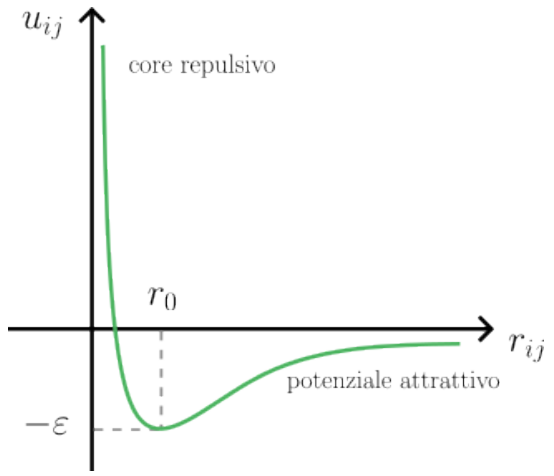
\includegraphics[width=0.4\linewidth]{Immagini/potenziale coefficiente a2.png}
    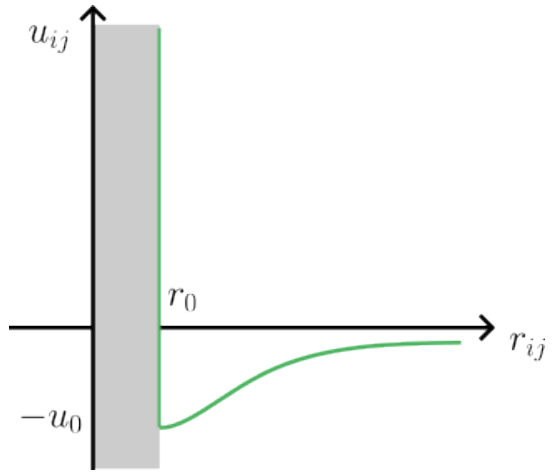
\includegraphics[width=0.4\linewidth]{Immagini/potenziale coefficiente a2 hardcore.png}
    \caption{potenziale intermolecolare di Lennard - Jones e la sua approssimazione ``hardcore''.}
    \label{fig: potenziale coefficiente a2}
\end{figure}
Dato che il potenziale dipende solo dalla distanza reciproca, allora è conveniente cambiare variabili in quelle del centro di massa avente jacobiano unitario
\begin{equation}
    \begin{cases}
        \vq_{CM} = \dfrac{1}{2}(\vq_1 + \vq_2) \\
        \vx = \vq_1 - \vq_2
    \end{cases},
\end{equation}
con le quali si ha
\begin{equation}
    \int d^3q_1\,d^3q_2\,f_{12}(r_{12}) = \int d^3q_{CM}\int d^3x\,f_{12}(|\vx|) = V\int d^3x\,f_{12}(|\vx|)
\end{equation}
e quindi, ricordando che la definizione $f_{ij} = e^{-\beta u_{ij}} - 1 $, si arriva a
\begin{equation}
    b_2 = \frac{V}{2VV_T}\int d^3x\,f_{12}(|\vx|) = \frac{1}{2V_T}\int d^3x\,[e^{-\beta u(|\vx|)} - 1].
\end{equation}
Passando adesso in coordinate in polari e tenendo conto della forma del potenziale \eqref{eq: potenziale Lennard-Jones approx.} si ha
\begin{equation}
    \begin{split}
        b_2 &= \frac{2\pi}{V_T}\int_0^\infty dr\,r^2[e^{-\beta u(r)} - 1] \\
        &= \frac{2\pi}{V_T}\bigg\{-\int_0^{r_0}dr\,r^2 + \int_{r_0}^\infty dr\,r^2[e^{\beta u_0(r_0/r)^6} - 1]\bigg\}.
    \end{split} 
\end{equation}
Per l'ipotesi sull'intensità dell'interazione $\beta u_{ij} \ll 1$, il secondo integrale è approssimare con
\begin{equation}
    e^{\beta u_0(r_0/r)^6} - 1 \simeq \beta u_0\bigg(\frac{r_0}{r}\bigg)^6,
\end{equation}
rimanendo con
\begin{equation}
\label{eq: coefficiente b2}
    \begin{split}
        b_2 &\simeq \frac{2\pi}{V_T}\bigg[-\frac{r_0^3}{3} + \beta u_0r_0^6\int_{r_0}^\infty \frac{dr}{r^4}\bigg] \\
        &= \frac{2\pi}{V_T}\bigg[-\frac{r_0^3}{3} - \frac{\beta u_0r_0^6}{3}\frac{1}{r^3}\bigg|_{r_0}^\infty\bigg] \\
        &= -\frac{2\pi}{3V_T}r_0^3(1 - \beta u_0).
    \end{split} 
\end{equation}
Sostituendo quanto ottenuto per $b_2$ in \eqref{eq: coefficiente b2} nell'equazione di stato \eqref{eq: equazione di stato (espansione viriale)}, tenendo conto che $a_2 = -b_2$, si trova la prima correzione viriale
\begin{equation}
\label{eq: equazione di stato (I corezione viriale)}
    pV \simeq kT\vmedio{N}\bigg[1 + \frac{2\pi r_0^3}{3v}\bigg(1 - \frac{u_0}{kT}\bigg)\bigg].
\end{equation}
Per quanto vi siano forti approssimazioni in questa derivazione, l'equazione di stato ottenuta è equivalente all'equazione di Van der Waals \eqref{eq: equazione di stato Van der Waals}, la quale è fenomenologicamente valida in questo regime. Infatti, si riscrive la \eqref{eq: equazione di stato (I corezione viriale)} come la relazione
\begin{equation}
    p + \frac{2\pi u_0r_0^3}{3v^2} = \frac{kT}{v}\bigg(1 + \frac{2\pi r_0^3}{3v}\bigg).
\end{equation}
Siccome si è considerato il limite di bassa densità, il volume disponibile $v$ per ogni particella deve essere molto più grande del volume escluso $r_0^3$, per cui si può dire che $r_0^3/v \ll 1$ e scrivere il secondo termine della relazione precedente come
\begin{equation}
    \bigg(1 - \frac{2\pi r_0^3}{3v}\bigg)^{-1} \simeq \frac{v}{v - 2\pi r_0^3/3},
\end{equation}
arrivando quindi a 
\begin{equation}
     \bigg(p + \frac{2\pi u_0r_0^3}{3v^2}\bigg)\bigg(v - \frac{2\pi r_0^3}{3}\bigg) = kT,
\end{equation}
che, ponendo $A \equiv 2\pi u_0r_0^3/3$ e $B \equiv 2\pi r_0^3/3$, coincide proprio con l'equazione di Van der Waals
\begin{equation}
    \bigg(p + \frac{a}{V^2}\bigg)(V - b) = NkT.
\end{equation}
\begin{obs}
    Nella \eqref{eq: equazione di stato Van der Waals} si era posto il numero di moli pari ad uno, per trovare un identico risultato basta definire $A = a/N^2$ e $B = b/N$.
\end{obs}
Si ricorda che l'interpretazione del parametro $B$ era quella di volume per particella ``escluso'' a causa del volume finito delle molecole. Effettivamente, anche ora compare il volume escluso $r_0^3$ che corrisponde ad una sfera di diametro $r_0$ e quindi di un volume
\begin{equation}
    \frac{4\pi}{3}\bigg(\frac{r_0}{2}\bigg)^3 = \frac{B}{4}.
\end{equation}
Il parametro $A$ era attribuito all'effetto dell'interazione attrattiva, e questo è confermato dalla proporzionalità con $u_0$. L'equazione di Van der Waals è dunque ottenuta da un'espansione perturbativa al primo ordine, quindi è valida solo nel limite di alte temperature. Se si volesse studiare il limite a basse temperature si dovrebbero incorporare correzioni successive che modificherebbero l'equazione di stato, che alla fine dovrebbe mostrare addirittura una transizione di fase. Quindi, quando le interazioni diventano rilevanti rispetto all'energia termica $kT$, l'equazione di Van der Waals non è più giustificata. Ecco perché questa equazione porta a conclusioni non fisicamente accettabili al di sotto di una temperatura critica; in particolare, viene violata la condizione di stabilità
\begin{equation}
    \frac{\p p}{\p V}\bigg|_{T,N} \le 0,
\end{equation}
che, con la costruzione di Maxwell, corrisponde alla comparsa di una transizione di fase. Questa non può venire catturata semplicemente da un'espansione perturbativa, nemmeno andando ad ordini più alti nell'espansione. Per ricavare esplicitamente le transizioni di fase dalla descrizione della Meccanica statistica sono necessarie soluzioni esatte, o quanto meno metodi non perturbativi. I primi risultati importanti riguardo alla spiegazione delle transizioni di fase furono ottenuti nell'ambito delle transizioni ferromagnetiche, con il modello di Ising.
\chapter{Teoria di Lee - Yang e Modello di Ising}
Uno dei contributi più importanti in Meccanica statistica per comprendere le transizioni di fase proviene dalla teoria di Lee - Yang riguardante la struttura generale della funzione di partizione canonica. In particolare, i teoremi di Lee - Yang dimostrano come le transizioni di fase emergano solamente nel limite termodinamico. Per semplicità, ci si limita alla trattazione classica, ma con le medesime assunzioni anche la trattazione quantistica porterebbe agli stessi risultati. 

Si parte riconsiderando un potenziale di interazione della forma vista nella \eqref{eq: potenziale Lennard-Jones approx.} e in figura \ref{fig: potenziale coefficiente a2}, essenzialmente si considerano le componenti del sistema come sfere di volume $v_0 \propto r_0^3$. Questo implica che finché il sistema è contenuto in un volume finito $V$, deve esistere un numero massimo di particelle $M$ tale per cui $N \le M$, dove $M = V/v_0$. Di conseguenza, la funzione di partizione grancanonica non è definita sull'intervallo $[0,\infty)$, ma su $[0,M]$ come
\begin{equation}
    Q = \sum_{N = 0}^M \frac{1}{N!}\bigg(\frac{z}{V_T}\bigg)^N\intconfig.
\end{equation}
Per convenienza, si definisce la variabile 
\begin{equation}
    y \equiv \frac{z}{V_T} = \frac{e^{\beta\mu}}{V_T},
\end{equation}
quindi per un volume finito $V$ la funzione di partizione grancanonica è un polinomio di grado $M$ in $y$ a coefficienti positivi
\begin{equation}
\label{eq: funzione di partizione grancanonica LY}
    Q = \sum_{N = 0}^M \frac{y^N}{N!}\intconfig.
\end{equation}
La regione fisica si ha per valori di $y$ reali e positivi, dato che è definita come il rapporto tra un esponenziale e un volume. Tuttavia, un polinomio a coefficienti positivi non ha alcuna radice reale positiva, per cui si hanno le relazioni
\begin{equation}
\label{eq: proprietà funzione di partizione grancanonica LY}
    Q > 1,\quad y\frac{\p Q}{\p y} > 1.
\end{equation}
Per il teorema fondamentale dell'algebra, il polinomio $Q$ può essere fattorizzato nel piano complesso come
\begin{equation}
    Q  = \prod_{i=1}^M\bigg(1 - \frac{y}{\bar{y}_i}\bigg),
\end{equation}
dove $\bar{y}_i \notin \R^+_0$ sono le radici di $Q$. A partire dalla funzione di partizione grancanonica \eqref{eq: funzione di partizione grancanonica LY}, si possono ricavare come al solito derivare le quantità termodinamiche passando dal potenziale grancanonico $\varpi = -kT\log{Q}$; quindi, la pressione è data da
\begin{equation}
    p = \frac{kT}{V}\log{Q},
\end{equation}
mentre la densità è data da 
\begin{equation}
    \frac{\vmedio{N}}{V} = -\frac{1}{kTV}z\frac{\p\varpi}{\p z}\bigg|_{T,V} = \frac{y}{V}\frac{\p\log{Q}}{\p y}\bigg|_{T,V},
\end{equation}
dove si è usato il fatto, per definizione di $y$, che 
\begin{equation}
    z\frac{\p}{\p z}\bigg|_{T,V} = y\frac{\p}{\p y}\bigg|_{T,V}.
\end{equation}
Pertanto, pressione e densità sono legate dalla relazione 
\begin{equation}
    \frac{\vmedio{N}}{V} = y\frac{\p}{\p y}\bigg(\frac{p}{kT}\bigg),
\end{equation}
inoltre dalle proprietà di $Q$ riportate nella \eqref{eq: proprietà funzione di partizione grancanonica LY} si deduce che pressione e densità sono funzioni regolari di $y$, ossia insieme alle loro derivate sono prive di singolarità, e che
\begin{equation}
    p>0,\quad \frac{\vmedio{N}}{V} > 0, \quad \frac{\p p}{\p y} > 0,\quad \frac{\p }{\p y}\bigg(\frac{\vmedio{N}}{V}\bigg) > 0;
\end{equation}
pertanto, la condizione di stabilità è sempre soddisfatta 
\begin{equation}
\label{eq: condizione stabilità LY}
    \frac{\p p}{\p v} < 0,
\end{equation}
ma allora se il volume è finito non si osserva alcuna transizione di fase. Tuttavia, le cose cambiano nel limite in cui $V \to \infty$, in quanto il numero di particelle non è più limitato superiormente da $M$ e $Q$ da un polinomio di grado finito passa ad essere una serie con la possibilità di sviluppare della singolarità. Quindi, nel limite termodinamico si considera il limite per $V \to \infty$ della pressione e della densità 
\begin{equation}
    \begin{cases}
        \dfrac{p}{kT} = \displaystyle\lim_{V\to\infty}{\dfrac{\log{Q}}{V}} \\[2ex]
        \dfrac{\vmedio{N}}{V} = \displaystyle\lim_{V\to\infty}{\dfrac{y}{V}\dfrac{\p\log{Q}}{\p y}\bigg|_{T,V}}
    \end{cases},\quad Q \equiv Q(T,V,y),
\end{equation}
osservando che adesso per ricavare una relazione che leghi le due quantità si dovrebbe scambiare l'ordine del limite con la derivata, ma in generale non è detto che nel limite considerato questi due operatori commutino a causa della possibile presenza di singolarità. Quindi, in generale si ha che 
\begin{equation}
    \frac{1}{v} = \lim_{V\to\infty}{\bigg(\dfrac{y}{V}\dfrac{\p\log{Q}}{\p y}\bigg)\bigg|_{T,V}} \neq y\frac{\p}{\p y}\bigg( \lim_{V\to\infty}{\frac{\log{Q}}{V}\bigg)\bigg|_{T,V}}
\end{equation}
e di conseguenza non è sempre garantita la condizione di stabilità \eqref{eq: condizione stabilità LY}. 

\section{Teoremi di Lee - Yang}
In realtà, Lee e Yang hanno dimostrato con i loro teoremi che esistono delle regioni nel piano complesso in cui la derivata rispetto ad $y$ e il limite per $V \to \infty$ commutano. In particolare, per le interazioni che si considerano qui, Lee e Yang hanno dimostrato due teoremi i cui enunciati è il seguente. 
\begin{teo}[primo teorema di Lee - Yang]
\label{teo: I teo LY}
    Per valori di $y \in \R^+$, ossia per valori fisicamente rilevanti di $y$, la funzione 
    \begin{equation}
        \frac{\log{Q}}{V}
    \end{equation}
    tende nel limite termodinamico $V\to\infty$ ad una funzione crescente monotona di $y$ che non dipende dalla forma\footnote{A meno che il volume $V$ abbia una forma tale che la superficie esterna cresca con$V$ più rapidamente di $V^{2/3}$.} del volume $V$.
\end{teo}
\begin{teo}[secondo teorema di Lee - Yang]
\label{teo: II teo LY}
    In ogni regione $\region$ del piano complesso $\C$ contenente un tratto dell'asse reale positivo in cui non sono presenti radici del polinomio $Q$, anche nel limite termodinamico $V \to \infty$ le quantità
    \begin{equation}
        \frac{\log{Q}}{V},\quad y\frac{\p}{\p y}\bigg(\frac{\log{Q}}{V}\bigg),\quad \bigg(y\frac{\p}{\p y}\bigg)^2\bigg(\frac{\log{Q}}{V}\bigg),\quad\dots
    \end{equation}
    tendono a funzioni di $y$ ben definite ed analitiche, ossia prive di singolarità.
\end{teo}
Pertanto, in una regione $\region$ per cui vale il teorema \eqref{teo: II teo LY}, la derivata in $y$ e il limite per $V \to \infty$ commutano, rendendo valida la relazione
\begin{equation}
    \frac{1}{v} = y\frac{\p}{\p y}\bigg(\frac{p}{kT}\bigg).
\end{equation}
Quindi, con la validità di tutte le manipolazioni del caso con volume $V$ finito, nella regione $\region$ si giunge ad un'equazione di stato ben definita e con la condizione di stabilità \eqref{eq: condizione stabilità LY} rispettata. In altre parole, in ogni regione $\region$ il sistema è in una specifica fase termodinamica. 

Dunque, facendo un po' di chiarezza, nel caso di un volume $V$ finito si era detto che sull'asse reale positivo non sono presenti radici di $Q$, quindi in questo frangente la regione $\region$ coincide con tale semiasse, il sistema può presentarsi in un'unica fase termodinamica e non può avvenire alcuna transizione di fase; invece, nel caso di un volume $V \to \infty$ il polinomio $Q$ passa ad essere una serie e il suo numero di radici $\bar{y}_i$ diventa infinito, la cui posizione, dipendente da $T$ e $V$, può portare a dei punti di accumulazione sull'asse reale positivo e generare diverse regioni $\region$ per cui valgono i teoremi di Lee - Yang. Un esempio di situazione può essere quello mostrato in figura \ref{fig: regioni di LY}, dove in ciascuna delle tre regioni $\region_1$, $\region_2$ e $\region_3$ valgono tali teoremi e dove il sistema assume fasi termodinamiche diverse.
\begin{figure}[h]
    \centering
    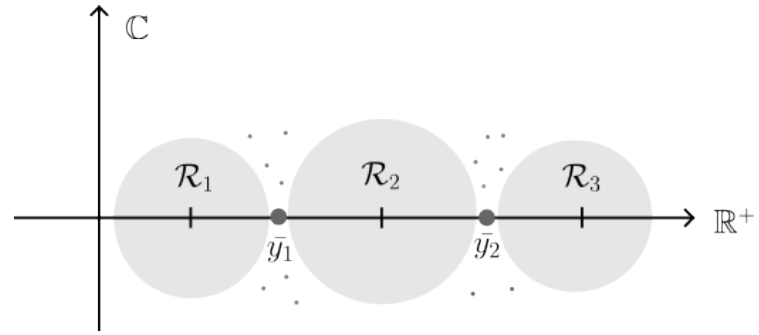
\includegraphics[width=0.55\linewidth]{Immagini/regioni di LY.png}
    \caption{esempio di sistema che può assumere tre fasi distinte associate alle regioni $\region$ rispettive.}
    \label{fig: regioni di LY}
\end{figure}
Al variare di $T$ può accadere per un certo valore critico $T_c$ che una radice lasci l'asse reale positivo; se ad esempio questo accade con $\bar{y}_1$, le regioni $\region_1$ e $\region_2$ si uniscono rimuovendo la possibilità di transizione al sistema tra le fasi associate ad esse. 

Ci si concentri adesso sul limite $V \to \infty$. Il teorema \eqref{teo: I teo LY} implica che la pressione  rimane continua anche nei punti corrispondenti alle radici $\bar{y}_i$ di $Q$, ma il secondo teorema \eqref{teo: II teo LY} si applica separatamente alle regioni $\region$ e pertanto la densità in generale non è continua in tali punti. Quindi, fissare dei valori di $y$ corrisponde a fissare dei valori per il potenziale chimico e la situazione che si presenta è del tipo mostrata in figura \ref{fig: andamento p(y) e p(v) (LY)}: invertendo la relazione tra la densità $1/v$ e $y$ segue un digramma $(p,V)$ a temperatura fissata che mostra delle transizioni di fase. 
\begin{figure}[h]
    \centering
    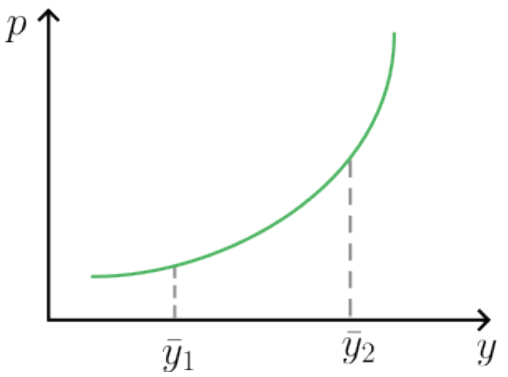
\includegraphics[width=0.3\linewidth]{Immagini/andamento p(y) (LY) 1.png}
    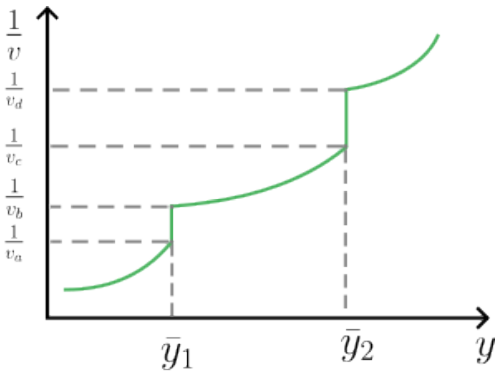
\includegraphics[width=0.3\linewidth]{Immagini/andamento p(y) (LY) 2.png}
    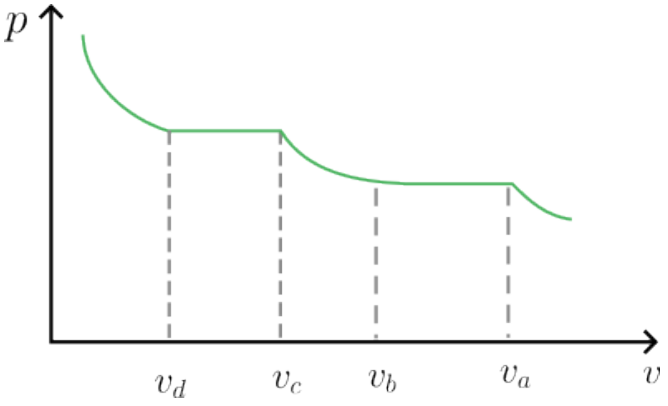
\includegraphics[width=0.35\linewidth]{Immagini/andamento p(v) (LY).png}
    \caption{andamento: (i) di $p$ in funzione di $y$; (ii) di $1/v$ in funzione di $y$; di $p$ in funzione di $v$.}
    \label{fig: andamento p(y) e p(v) (LY)}
\end{figure}
Si nota che in ogni regione $\region_i$ la particolare equazione di stato determina un altrettanto particolare espressione di $y \equiv y(T,V,N)$ e quindi di $\mu \equiv \mu(T,V,N)$, quando il potenziale chimico è considerato come variabile indipendente. Nei punti $\bar{y}_i$ corrispondenti alle transizioni i potenziali chimici coincidono, che è esattamente quanto richiesto dalla condizione per la coesistenza di fasi diverse \eqref{eq: condizione coesistenza}. 
\begin{obs}
    Lee e Yang hanno mostrato rigorosamente che questo meccanismo nel caso del ``lattice gas model'' è isomorfo al modello di Ising.
\end{obs}

\subsection{Transizioni continue del secondo ordine}
In Termodinamica, si è insistito in particolare sulle transizioni di fase del primo ordine tra due fasi che differiscono qualitativamente in modo profondo, come fase solida e liquida. Tuttavia, sono estremamente interessanti in vari ambiti anche le transizioni continue, in particolare in quelle del secondo ordine, come quella che avviene al punto critico dell'acqua. In queste transizioni i concetti chiave sono quelli di ``rottura spontanea di simmetria'' e di ``parametro d'ordine''. L'hamiltoniana microscopica è invariante rispetto ad un gruppo di simmetria $G$, che potrebbe essere ad esempio il gruppo delle rotazioni. Quello che succede per queste transizioni tipicamente è che:
\begin{enumerate}
    \item per $T > T_c$, lo stato macroscopico del sistema è invariante sotto trasformazioni di $G$ e si trova pertanto nella ``fase disordinata'' dove la simmetria è completamente conservata;
    \item per $T < T_c$, lo stato macroscopico del sistema è invariante sotto trasformazioni di un sottogruppo $G' \le G$ detto ``gruppo di stabilità'' e si trova pertanto ``fase ordinata'' dove avviene una rottura spontanea della simmetria. 
\end{enumerate}
Invece, un parametro d'ordine è una qualsiasi osservabile $O$ invariante sotto $G$ e che quindi ha valore medio nullo nella fase disordinata $\vmedio{O}_{D} = 0$, ma con valore medio non nullo nella fase ordinata $\vmedio{O}_O \neq 0$, il quale indica la rottura della simmetria.

\subsubsection{Transizione ferromagnetica}
Un esempio di rottura di simmetria è dato dalla transizione da ferromagnete a paramagnete alla temperatura critica di Curie $T_c$, in assenza di campo magnetico esterno. In questo caso il parametro d'ordine è la magnetizzazione $\vM$ che, essendo un vettore, in assenza di una direzione privilegiata il suo valore di aspettazione deve essere uguale a zero. Invece, quando avviene una rottura di simmetria e si ha una direzione privilegiata, non si ha più invarianza per rotazioni, ma solo rispetto al sottogruppo $SO(2)$. 
\begin{figure}[h]
    \centering
    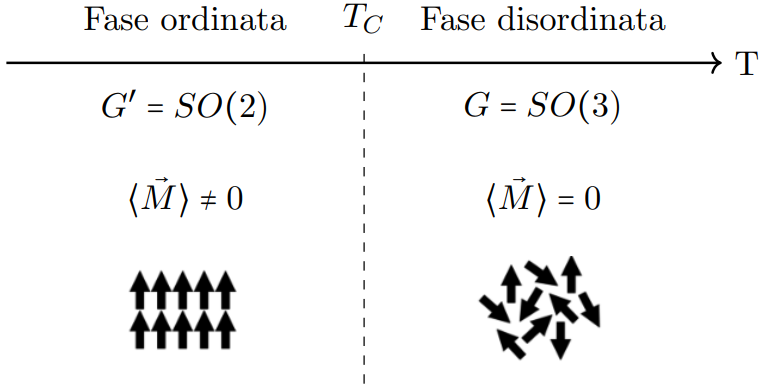
\includegraphics[width=0.53\linewidth]{Immagini/confronto fase ordinata - disordinata.png}
    \caption{confronto tra la fase ordinata e quella disordinata, con gruppi di simmetria relativi.}
    \label{fig: confronto fase ordinata - disordinata}
\end{figure}
\begin{obs}
    Una rappresentazione drasticamente semplificata dei sistemi ferromagnetici reali è data dal modello di Ising, il quale riesce a catturare comunque gli aspetti essenziali; in particolare, esso esibisce esplicitamente la transizione di fase ferromagnetica.
\end{obs}

\subsubsection{Proprietà di universalità}
Il fatto che anche un modello molto semplificato come quello di Ising catturi correttamente le caratteristiche di questa transizione continua del secondo ordine è legato al concetto di universalità, riguardante il comportamento del sistema nel limite per $T \to T_c$. Si definisce la temperatura ridotta $t$ come
\begin{equation}
    t := \frac{T - T_c}{T_c},
\end{equation}
la quale quantifica la vicinanza di $T$ alla temperatura critica $T_c$. Nelle transizioni del secondo ordine, le quantità termodinamiche seguono delle leggi di potenza per $|t| \to 0$; ad esempio, per la transizione ferromagnetica, avvicinandosi a $T_c$ dalla fase ordinata, ossia con $T < T_c$ e $t < 0$, la magnetizzazione spontanea $M \equiv \vmedio{\vM}$ tende a zero secondo 
\begin{equation}
\label{eq: legge di potenza magnetizzazione}
    M \propto (-t)^\beta.
\end{equation}
\begin{notz}
    In questo contesto, il parametro $\beta$ in \eqref{eq: legge di potenza magnetizzazione} non ha nulla a che fare con il parametro $\beta = 1/kT$.
\end{notz}
Invece, la suscettività magnetica $\chi$ e il calore specifico $c_{V}$ divergono secondo
\begin{equation}
\label{eq: legge di potenza suscettività e calore specifico}
    \chi \propto |t|^{-\gamma},\quad c_V \propto |t|^{-\alpha}.
\end{equation}
Gli esponenti $\alpha$, $\beta$ e $\gamma$ prendono il nome di ``indici critici'' e caratterizzano il comportamento del sistema nei pressi del punto critico; inoltre, non dipendono dai dettagli del sistema, ma da caratteristiche generali come i pattern di rottura di simmetria che provocano la riduzione $G \to G'$ e la dimensionalità $D$ dello spazio. Queste caratteristiche generali determinano classi di universalità dei sistemi fisici, i quali possono essere tra loro molto diversi come composizione microscopica, caratterizzata da un certo insieme di indici critici.

\section{Modello di Ising}
Nei materiali ferromagnetici reali gli atomi formano un reticolo più o meno regolare e sono dotati di spin, quindi di un momento magnetico $\bm{\mu}_B$. Tali momenti magnetici interagiscono fra di loro e percepiscono anche l'influenza di un campo magnetico esterno di intensità $B$. Nel modello semplificato si può assumere che:
\begin{enumerate}
    \item il reticolo è regolare, considerabile normalmente un ipercubo;
    \item ad ognuno degli $N$ siti reticolari è associata una variabile dinamica $s_i = \pm 1$, con $i = 1,\dots,N$, che rappresenta i due possibili autovalori della terza componente di $\mu_B$, se lo spin è pari ad $1/2$;
    \item un microstato del sistema corrisponde ad assegnare un insieme di variabili $\{s_i\}$ e il numero di possibili microstati $n$ è pari a $n = 2^N$, dato che in ogni sito si hanno due possibili scelte;
    \item due momenti magnetici $s_i$ ed $s_j$ interagiscono solo se $\vmedio{ij}$ è un ``link'', ossia solo se i due momenti sono primi vicini nel reticolo;
    \item le variabili $s_i$ interagiscono anche con un campo magnetico esterno $B$ presente in ogni punto tramite $h = \mu_BB$;
    \item l'hamiltoniana del modello è 
    \begin{equation}
    \label{eq: hamiltoninana modello di Ising}
        H = -J\sum_{\vmedio{ij}}s_is_j - h\sum_{i=1}^Ns_i,
    \end{equation}
    dove $J$ è il parametro macroscopico che determina l'intensità dell'accoppiamento tra gli spin primi vicini e il secondo termine di interazione tende ad allineare gli spin con il campo magnetico $B$ esterno;
    \item per descrivere un materiale ferromagnetico si pone $J > 0$.
\end{enumerate}
L'energia interna è più bassa se in un link $\vmedio{ij}$ i due spin $s_i$ ed $s_j$ sono concordi, cioè se $s_is_j = 1$; quindi, l'allineamento reciproco degli spin è favorito energeticamente e il secondo termine dell'hamiltoninana \eqref{eq: hamiltoninana modello di Ising} favorisce l'allineamento degli spin con il campo $h$. Essenzialmente, l'hamiltoniana fa tendere il sistema alla fase ordinata allineando tutti gli spin, mentre l'entropia svolge il ruolo opposto favorendo il disordine. Lo stato fondamentale di minima energia corrisponde a:
\begin{enumerate}
    \item quello in cui $s_i = 1$ per ogni $i$, se $h > 0$;
    \item quello in cui $s_i = -1$ per ogni $i$, se $h < 0$;
\end{enumerate}
Chiaramente, in assenza del campo esterno $h$ si hanno stati di energia minima sia che gli $s_i$ siano tutti allineati ``up'', cioè con $s_i = 1$, sia che siano tutti allineati ``down'', cioè con $s_i = -1$; per cui se $h = 0$ lo stato fondamentale è degenere. 

La funzione di partizione è data dalla somma su tutte le configurazioni, ossia su tutte le possibili scelte della variabile dinamica $s_i$ in ogni sito del reticolo, quindi
\begin{equation}
    Z = \sum_{\{s_i\}}e^{-\beta H(\{s_i\})}.
\end{equation}
Le variabili di controllo, oltre il numero di siti $N$ che viene tenuto fissato, sono la temperatura $T$ e il campo esterno $h$, entrambe intensive. Siccome il modello è definito su un reticolo, il volume $V$ non assume alcun ruolo. Ponendo $Z \equiv Z(T,h,N) = e^{-\beta G(T,h,N)}$, la funzione $G$ rappresenta, nel limite termodinamico, il potenziale appropriato alla scelta dell'insieme di variabili di controllo $\{T,h,N\}$, da non confondere con l'energia di Gibbs, anche se ci assomiglia. La variabile estensiva coniugata al campo $h$ è la magnetizzazione totale $M$, ottenuta a partire da $G$ tramite
\begin{equation}
\label{eq: magnetizzazione come media spin}
    \begin{split}
        M = -\frac{\p G}{\p h}\bigg|_{T,N} = \frac{1}{\beta}\frac{\p}{\p h}(\log{Z})\bigg|_{T,N} &= \frac{1}{\beta Z}\frac{\p}{\p h}\sum_{\{s_i\}}e^{-\beta H} \\
        &= -\frac{1}{Z}\sum_{\{s_i\}}\frac{\p H}{\p h}e^{-\beta H} \\
        &= \sum_{\{s_i\}}\bigg(\sum_{i=1}^N s_i\bigg)\frac{e^{-\beta H(\{s_i\})}}{Z} \\
        &= \bigvmedio{\sum_{i=1}^N s_i},
    \end{split}
\end{equation}
la quale quindi corrisponde al valore medio della somma degli spin $s_i$.

\subsubsection{Simmetria $\Z_2$}
Si consideri il caso in cui $h = 0$, l'hamiltoniana si riduce a $H = -J\sum_{\vmedio{ij}}s_is_j$ ed è invariante sotto trasformazioni di parità
\begin{equation}
    \Pi : s_i \longrightarrow -s_i,\quad \forall i.
\end{equation}
Questa operazione definisce il gruppo di simmetria $\Z_2$ dato che applicare due volte una trasformazione di parità restituisce l'oggetto iniziale, in termini operatoriali $\Pi^2 = \MI$. L'osservabile $\sum_is_i$ rappresenta un parametro d'ordine, infatti essa non è invariante sotto l'azione di $\Z_2$ in quanto 
\begin{equation}
    \Pi : \nsum_is_i \longrightarrow -\bigg(\nsum_is_i\bigg).
\end{equation}
Quindi, il valore medio $M = \vmedio{\nsum_is_i}$ non nullo indica una rottura della simmetria del gruppo $\Z_2$, spontanea perché invece l'hamiltoniana è invariante sotto l'azione di tale gruppo come detto prima. Se il numero $N$ di siti reticolari è finito, la rottura spontanea di simmetria non può avvenire, in quanto $s_i = \pm 1$ e sommare su tutte le possibili configurazioni degli $s_i$ o dei $\tilde{s}_i \equiv -s_i$ è del tutto equivalente. Pertanto, si può scrivere la relazione
\begin{equation}
    M = \sum_{\{s_i\}}\bigg(\sum_{i=1}^N s_i\bigg)\frac{e^{-\beta H(\{s_i\})}}{Z} = \sum_{\{\tilde{s_i}\}}\bigg(-\sum_{i=1}^N \tilde{s_i}\bigg)\frac{e^{-\beta H(\tilde{s_i})}}{Z},
\end{equation}
da cui, notando che le variabili $\{\tilde{s}_i\}$ sono mute essendo sono sommate, si può richiamare $\tilde{s}_i \to s_i$ e trovare che
\begin{equation}
    M = \sum_{\{s_i\}}\bigg(\sum_{i=1}^N s_i\bigg)\frac{e^{-\beta H(\{s_i\})}}{Z} = -\sum_{\{s_i\}}\bigg(\sum_{i=1}^N s_i\bigg)\frac{e^{-\beta H(\{s_i\})}}{Z} = -M,
\end{equation}
per cui necessariamente
\begin{equation}
    M  = 0.
\end{equation}
Quindi, le manipolazioni eseguite nel caso di $N$ finito sono sicuramente valide in quanto si ha a che fare con somme finite; invece, nel limite termodinamico, sorgono problemi riguardanti le condizioni al contorno e di convergenza che in linea di principio possono invalidare tali manipolazioni e permettere la comparsa di una fase ordinata in cui la simmetria $\Z_2$ viene rotta rendendo $M \neq 0$. Tutto ciò è analogo a quanto è emerso dalla teoria di Lee - Yang: le transizioni di fase sono legate a punti di non analiticità della funzione di partizione, siccome i singoli addendi della funzione di partizione sono analitici in $\beta$, tale è anche la loro somma, a meno che vi siano infiniti addendi e la somma diventi una serie.

Analogamente, in presenza del campo esterno $h$, la simmetria di $\Z_2$ mappa il modello microscopico in un modello per il campo $-h$, ovvero adesso
\begin{equation}
    H(\{s_i\},h) =  H(\{\tilde{s}_i\},-h).
\end{equation}
Dato che continua a valere l'equivalenza sulle operazioni di somma $\sum_{\{s_i\}} = \sum_{\{\tilde{s}_i\}}$, questo implica che
\begin{equation}
    Z(T,h,N) = Z(T,-h,N),\quad G(T,h,N) = G(T,-h,N),
\end{equation}
mentre per la magnetizzazione che
\begin{equation}
    M(T,h,N) = - M(T,-h,N).
\end{equation}
Il modello di Ising per quanto semplificato, cattura l'essenza della rottura spontanea di simmetria $\Z_2$. Si vedrà infatti che esso prevede, per reticoli in dimensione $D > 1$, la transizione di fase ferromagnetica e la presenza di una fase ordinata, date le proprietà di universalità delle transizioni di fase del secondo ordine.

\section{Lattice gas model}
Il modello di Ising è isomorfo al modello semplificato ``lattice gas model'' per un gas classico interagente, usato come punto di partenza per lo studio delle transizioni gas-liquido. Sia $V$ il volume occupato dal gas e lo si suddivida in $N$ celle elementari di volume $v_0$. Si ipotizza che questo gas non sia libero, ma sia caratterizzato da un potenziale di interazione intermolecolare che non permetta la sovrapposizione tra le particelle, come quello usato nella \eqref{eq: potenziale Lennard-Jones approx.}. Quindi, ogni cella può essere occupata al più da una singola particella di volume $v_0$ e il volume totale $V$ occupato dal gas si può esprimere come $V = Nv_0$. Si suppone inoltre che il potenziale di interazione risulti attrattivo per particelle molto vicine. In questa trattazione estremamente approssimata si trascura l'energia cinetica delle particelle, per cui il modello va applicato per temperature non eccessivamente alte, risultando non particolarmente adeguato a descrivere il sistema nel limite classico. 

Nell'ensemble grancanonico, il numero di particelle $N_p$ può fluttuare e ogni microstato $\nu$ corrisponde alla collezione di numeri di occupazione $\{n_i\}$ con $n_i = 0,1$ per $i = 1,\dots,N$. All'energia totale contribuiscono solo le particelle in celle continue, ossia prime vicine, quindi l'energia e il numero di particelle del microstato $\{n_i\}$ sono date da
\begin{equation}
    E(\{n_i\}) = -\epsilon\sum_{\vmedio{ij}}n_in_j,\quad N_p(\{n_i\}) = \sum_{i=1}^Nn_i.
\end{equation}
Pertanto, la funzione di partizione grancanonica è
\begin{equation}
\label{eq: funzione di partizione lattice gas model (grancanonico)}
    Q(T,V,\mu) = \sum_{\{n_i\}}\exp{\bigg(\beta\epsilon\sum_{\vmedio{ij}}n_in_j + \beta\mu\sum_{i=1}^Nn_i\bigg)}.
\end{equation}
La corrispondenza tra il lattice gas model e il modello di Ising si può esprimere graficamente come in figura \ref{fig: relazione lattice gas model ed Ising}. 
\begin{figure}[h]
    \centering
    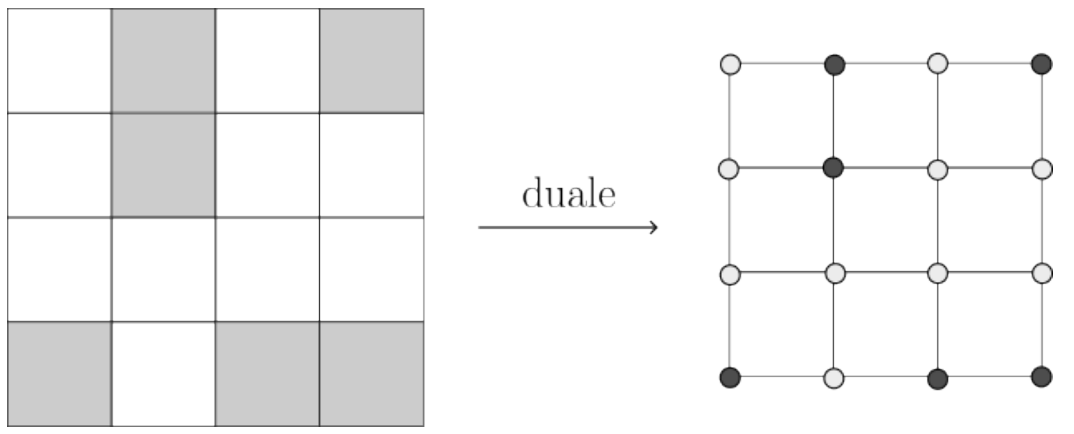
\includegraphics[width=0.7\linewidth]{Immagini/relazione lattice gas model ed Ising.png}
    \caption{corrispondenza tra il lattice gas model ed il modello di Ising.}
    \label{fig: relazione lattice gas model ed Ising}
\end{figure}
Tutte le configurazioni degli $n_i$ si possono mappare in configurazione del modello di Ising prendendo il modello duale a quello delle celle facendo corrispondere $n_i = 1 \to s_i = 1$ e $n_i = 0 \to s_i = -1$, esplicitamente
\begin{equation}
\label{eq: I corrispondenza LGM e MI}
    s_i = 2n_i - 1\quad\longleftrightarrow\quad n_i = \frac{s_i + 1}{2}.
\end{equation}
Rispetto a questa corrispondenza, l'esponente nella funzione di partizione \eqref{eq: funzione di partizione lattice gas model (grancanonico)} diventa
\begin{equation}
    \begin{split}
        \beta\epsilon\sum_{\vmedio{ij}}n_in_j + \beta\mu\nsum_in_i &= \beta\bigg[\frac{\epsilon}{4}\sum_{\vmedio{ij}}s_is_j + \bigg(\frac{\epsilon q}{2} + \frac{\mu}{2}\bigg)\sum_{i=1}^Ns_i + N\bigg(\frac{\epsilon q}{8} + \frac{\mu}{2}\bigg)\bigg] \\
        &= \beta H + \mathrm{costante},
    \end{split}
\end{equation}
dove $H$ è l'hamiltoniana del modello di Ising \eqref{eq: hamiltoninana modello di Ising} con parametri
\begin{equation}
\label{eq: II corrispondenza LGM e MI}
    J = \frac{\epsilon}{4},\quad h = \frac{1}{2}(\mu + \epsilon q),
\end{equation}
dove $q$ è il ``numero di coordinazione'' del reticolo, ossia il numero di siti primi vicini di un dato sito. Quindi, la differenza tra i due modelli corrisponde quindi ad una traslazione di una costante. Quest'ultima è indipendente dal microstato ed è irrilevante dato che viene riassorbito dalla normalizzazione della funzione di partizione non influenzando quindi la probabilità dei microstati e i valori medi delle osservabili. Dunque, il lattice gas model e il modello di Ising, con le corrispondenze \eqref{eq: I corrispondenza LGM e MI} e \eqref{eq: II corrispondenza LGM e MI}, sono equivalenti, ossia isomorfi. In particolare, vale l'equivalenza sulle operazioni di somma $\sum_{\{n_i\}} = \sum_{\{s_i\}}$, dato che le configurazioni sono mappate uno ad uno, quindi
\begin{equation}
    Q(T,V,\mu) = \mathrm{costante}\times Z(T,h,N).
\end{equation}
Inoltre, il numero medio di particelle nel lattice gas model è dato da
\begin{equation}
    \vmedio{N_p} = \bigvmedio{\sum_{i=1}^Nn_i} = \frac{1}{2}\bigvmedio{\sum_{i=1}^N(s_i + 1)} = \frac{M + N}{2}.
\end{equation}
La comparsa della magnetizzazione nel modello di Ising corrisponde, nel lattice gas model, ad una condensazione delle particelle in una fase liquida e quindi ad una transizione di fase. 

\section{Modello di Ising 1-dimensionale}
Il caso unidimensionale del modello di Ising è quello più semplice dove è possibile risolvere esattamente la funzione di partizione. Purtroppo, è anche il caso meno interessante dato che non mostra transizioni di fase: ogni spin ha troppi pochi primi vicini e quindi l'ordine non riesce a comparire con il disordine dovuto all'entropia. 
\begin{figure}[h]
    \centering
    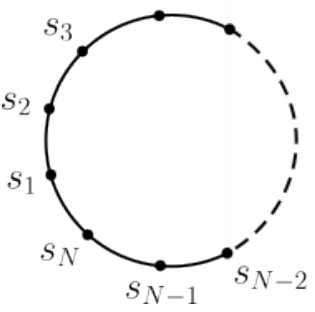
\includegraphics[width=0.25\linewidth]{Immagini/modello Ising D = 1.png}
    \caption{reticolo unidimensionale con condizione periodiche al contorno.}
    \label{fig: modello Ising D = 1}
\end{figure}
Come punto di partenza, si considera  un reticolo unidimensionale rappresentabile come una ``catena'' di spin; poi, si impongono delle condizioni al contorno periodiche\footnote{Si scelgono qui condizioni al contorno periodiche solamente per una questione di semplicità, ma in generale si possono usare anche altre condizioni al contorno senza particolari problemi.} rendendo così la catena chiusa con $s_1$ e $s_N$ primi vicini soddisfacenti la relazione $s_1 = s_{N+1}$, come si vede in figura \ref{fig: modello Ising D = 1}. Quindi, la funzione di partizione è data
\begin{equation}
    \begin{split}
        Z &= \sum_{\{s_i\}}\exp\bigg(\beta J\sum_{\vmedio{ij}}s_is_j + \beta h\sum_{i=1}^Ns_i\bigg) \\
        &= \sum_{\{s_i\}}\exp\bigg[\beta J\sum_{i=1}^Ns_is_{i+1} + \frac{\beta h}{2}\bigg(\sum_{i=1}^Ns_i + \sum_{i=1}^Ns_{i+1}\bigg)\bigg],
    \end{split}
\end{equation}
dove si è riscritto in modo simmetrico il secondo termine all'esponente e da cui si deduce che la struttura della catena implica
\begin{equation}
    \sum_{\vmedio{ij}}s_is_j = \sum_{i=1}^Ns_is_{i+1}.
\end{equation}
In questo modo si ha
\begin{equation}
    \begin{split}
        Z &= \sum_{\{s_i\}}\prod_{i=1}^N\exp{\bigg(\beta Js_is_{i+1} + \frac{\beta h}{2}s_i + \frac{\beta h}{2}s_{i+1}\bigg)} \\
        &= \sum_{\{s_i\}}\prod_{i=1}^N\TM_{s_i,s_{i+1}} \\
        &= \sum_{s_1,\dots,s_N}\underbrace{\TM_{s_1,s_2}\TM_{s_2,s_3}}_{=\TM^2_{s_1,s_3}}\cdots\TM_{s_{N-1},s_N}\TM_{s_N,s_1} \\
        &= \Tr{\TM^N},
    \end{split} 
\end{equation}
dove si è sfruttata la periodicità della catena e si è introdotta la ``matrice di trasferimento'' del sistema $\TM \equiv \TM_{s_i,s_{i+1}}$ definita come 
\begin{equation}
    \TM := 
    \begin{pmatrix}
        e^{\beta J + \beta h} & e^{-\beta J} \\
        e^{-\beta J} & e^{\beta J - \beta h}
    \end{pmatrix},
\end{equation}
la quale lega i possibili valori di un sito $s_i$ con i possibili valori di quello successivo $s_{i+1}$. La matrice $\TM$ può essere diagonalizzata risolvendo l'equazione caratteristica $\det{(\TM - \lambda\MI)} = 0$ che fornisce gli autovalori 
\begin{equation}
\label{eq: autovalori matrice trasferimento}
    \lambda_\pm = e^{\beta J}(\cosh{\beta h} \pm \sqrt{\cosh^2{(\beta h)} - 2e^{-2\beta J}\sinh{2\beta J}},\quad \lambda_+ > \lambda_-.
\end{equation}
Pertanto, la matrice di trasferimento è
\begin{equation}
    \TM^N = 
    \begin{pmatrix}
        \lambda_+^N & 0 \\
        0 & \lambda_-^N
    \end{pmatrix},
\end{equation}
per cui la funzione di partizione è
\begin{equation}
\label{eq: funzione di partizione Ising D=1}
    Z = \lambda_+^N + \lambda_-^N = \lambda_+^N\bigg[1 + \bigg(\frac{\lambda_-}{\lambda_+}\bigg)^N\bigg],
\end{equation}
che nel limite termodinamico si riduce semplicemente all'autovalore di $\TM$ maggiore
\begin{equation}
\label{eq: funzione di partizione Ising D=1 (limite TD)}
    Z \simeq \lambda_+^N,\quad N \to \infty.
\end{equation}
L'energia libera $G$, sempre in questo limite, è data da
\begin{equation}
    \begin{split}
        G &= -\frac{\log{Z}}{\beta} \\
        &=-N\bigg[J + \frac{1}{\beta}\log{\bigg(\cosh{\beta h} + \sqrt{\cosh^2{(\beta h)} - 2e^{-2\beta J}\sinh{2\beta J}}\bigg)}\bigg],
    \end{split}
\end{equation}
da cui si calcola la magnetizzazione
\begin{equation}
    M = -\frac{\p G}{\p h}\bigg|_{T,N} =  \frac{N\sinh{\beta h}}{\sqrt{\cosh^2{(\beta h)} - 2e^{-2\beta J}\sinh{2\beta J}}}.
\end{equation}
Se è presente un campo esterno, allora si genera una magnetizzazione, invece in assenza di questo, per $T \neq 0$, è sempre vera in $D = 1$ l'implicazione 
\begin{equation}
    h = 0\quad\Longrightarrow\quad M = 0.
\end{equation}
La magnetizzazione spontanea è sempre nulla e si è sempre nella fase disordinata in cui la simmetria di $\Z_2$ è conservata. Tuttavia, per reticoli $D$-dimensionali con $D > 1$ compare la transizione ferromagnetica, che non appare nel caso $1$-dimensionale a causa dell'influenza soppressa dei termini di accoppiamento che tendono ad allineare il sistema in quanto ogni sito ha solo due primi vicini. Sempre nel caso in cui $h = 0$, l'espressione esatta della funzione di partizione è un sottocaso dell'espressione generale \eqref{eq: funzione di partizione Ising D=1} con $\lambda_\pm$ dati dalla \eqref{eq: autovalori matrice trasferimento} che in assenza di campo esterno sono
\begin{equation}
    \lambda_+ = 2\cosh{\beta J},\quad \lambda_- = 2\sinh{\beta J},
\end{equation}
per cui la funzione di partizione è
\begin{equation}
    Z = (2\cosh{\beta J})^N + (2\sinh{\beta J})^N,
\end{equation}
da cui, trascurando nel limite termodinamico il secondo termine, si trova che l'energia libera vale
\begin{equation}
    G \simeq -\frac{N}{\beta}\log{(2\cosh{\beta J})},
\end{equation}
che per $T > 0$ è una funzione analitica, ossia priva di singolarità in $G$ e nelle sue derivate, pertanto non si presentano transizioni di fase. 
\begin{obs}
    Il modello di Ising 1-dimensionale con $h = 0$ può venire facilmente risolto anche con metodi diversi da quello della matrice di trasferimento. Tali metodi possono essere impiegati anche in dimensionalità $D$ generica e forniscono informazioni importanti anche se l'unico caso risolvibile esattamente, anche con $h = 0$, rimane quello bidimensionale.
\end{obs}

\section{Sviluppo ad alta temperatura per \texorpdfstring{$D = N$}{D = N}}
La tecnica che segue è applicabile quando il modello di Ising è definito tramite un qualsiasi grafo $G$, ossia su qualsiasi reticolo avente $N$ siti ai quali sono associate le variabili $s_i$ e $L$ link $\vmedio{ij}$ che collegano i siti continui, ossia i primi vicini. Se il reticolo è regolare, ossia se in ogni sito entra lo stesso numero $q$ di link, si ha che il numero di link è pari a
\begin{equation}
    L = \frac{Nq}{2},
\end{equation}
dove per ogni sito si sono considerati tutti i suoi primi vicini e si è diviso per due in modo da evitare di contare troppi link, ovviamente a parte per i siti sul bordo dato che possono avere un numero minore di primi vicini. Ad ogni link $\vmedio{ij}$ viene associato il fattore
\begin{equation}
\label{eq: identità sviluppo alta T}
    e^{\beta Js_is_j} \equiv e^{Ks_is_j},\quad K \equiv \beta J.
\end{equation}
Quindi, ciò che determina l'intensità dell'interazione nella funzione di partizione è un rapporto adimensionale tra l'energia di interazione e l'energia termica. Inoltre, vale l'identità
\begin{equation}
\label{eq: relazione exp(Ksisj) e cosh(K)}
    \begin{split}
        e^{Ks_is_j} = \cosh{K}(1  + s_is_j\tanh{K}) \equiv \cosh{K}(1  + s_is_jv),\quad v \equiv \tanh{K}.
    \end{split}
\end{equation}
Per considerare il limite di alta temperatura si assume $K \ll 1$, inoltre si prende $h = 0$ per semplicità, quindi la funzione di partizione è
\begin{equation}
    \begin{split}
        Z = \sum_{\{s_i\}}\exp{\bigg(K\sum_{\vmedio{ij}}s_is_j\bigg)} = \sum_{\{s_i\}}\prod_{\vmedio{ij}}e^{Ks_is_j} &= \sum_{\{s_i\}}\prod_{\vmedio{ij}}[\cosh{K}(1  + s_is_jv)] \\
        &= \cosh^L{(K)}\sum_{\{s_i\}}\prod_{\vmedio{ij}}(1  + s_is_jv).
    \end{split}
\end{equation}
Il prodotto sui link $\prod_{\vmedio{ij}}(1  + s_is_jv)$ è uno sviluppo che contiene $2^L$ termini, infatti si hanno due termini per ogni link: il termine dato da $1$ e quello con $v$; di questi può essere data una rappresentazione grafica tramite la notazione per i due possibili contributi del link $\vmedio{ij}$ in figura \ref{fig: notazione grafica prodotto link}. L'espansione del prodotto corrisponde all'espansione nei possibili sottografi di link attivi. 
\begin{figure}[h]
    \centering
    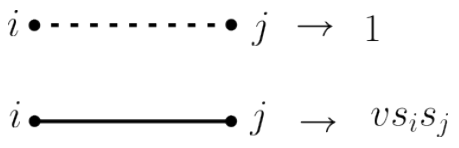
\includegraphics[width=0.35\linewidth]{Immagini/notazione grafica prodotto link.png}
    \caption{rappresentazione grafica dei termini del prodotto sui link: (i) link vuoto; (ii) link attivo.}
    \label{fig: notazione grafica prodotto link}
\end{figure}
\begin{ex}
    Se $G$ è un catena chiusa 1-dimensionale con $N = 3$ e $L = 3$, allora ci sono $2^3 = 8$ termini possibili, mostrati in figura \ref{fig: prodotto link con N = 3 ed L = 3 in D = 1}. Attraverso la somma dei triangoli si ottengono tutti i termini dello sviluppo; ad esempio, l'ultimo termine in figura corrisponde a tre link attivi per cui è dato da
    \begin{equation}
        (vs_1s_2)(vs_2s_3)(vs_3s_1) = v^3s_1s_2s_2s_3s_3s_1 = v^3,\quad s_i^2 = 1,\,i=1,2,3.
    \end{equation}
    \begin{figure}[H]
        \centering
        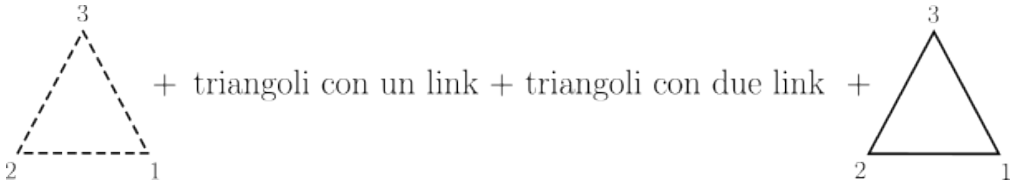
\includegraphics[width=0.75\linewidth]{Immagini/prodotto link con N = 3 ed L = 3 in D = 1.png}
        \caption{espansione del prodotto sui link per $N = 3$ ed $L = 3$ in $D = 1$.}
        \label{fig: prodotto link con N = 3 ed L = 3 in D = 1}
    \end{figure}
\end{ex}
Ci si concentri ora su un generico contributo di questa espansione. Nella funzione di partizione \eqref{eq: funzione di partizione Ising D=1} questo va sommato su tutti i possibili valori delle variabili $s_i$. Per un dato sito $i$, se $n_i$ è il numero di link attivi che entrano in tale sito, si ha la somma
\begin{equation}
    \sum_{s_i=\pm1}(s_i)^{n_i} = 
    \begin{cases}
        0,\quad n_i\ \mathrm{dispari} \\
        2,\quad n_i\ \mathrm{pari}\vee 0
    \end{cases}.
\end{equation}
Quindi, nella somma si devono scegliere i termini dello sviluppo in cui ogni variabile $s_i$ compare un numero pari di volte. Alla funzione di partizione contribuiscono dunque esclusivamente i sottografi in cui in ogni sito entra un numero pari di link attivi: tali configurazioni sono poligoni chiusi. Un dato poligono di lunghezza $l$, ossia contenente $l$ link attivi contribuisce con un termine pari a 
\begin{equation}
    2^Nv^l,
\end{equation}
infatti, in ogni sito del reticolo si ha un contributo pari a 2 poiché o non entrano link, e $n_i = 0$, o ne entra un numero pari, inoltre ad ogni link attivo si associa un contributo pari a $v$. Dunque, la funzione di partizione si può esprimere come
\begin{equation}
\label{eq: funzione di partizione Ising alta T}
    Z = 2^N\cosh^L{(K)}\sum_{l=0}^Lg_lv^l,
\end{equation}
dove $g_l$ è il numero di poligoni chiusi di lunghezza $l$ che possono essere tracciati sul grafo $G$. Il parametro di sviluppo $v$ è tale che $v \ll 1$ quando $\beta J \ll 1$, ossia quando $kT \gg J$. L'espressione \eqref{eq: funzione di partizione Ising alta T} costituisce quindi un'espansione perturbativa, valida per alte temperature\footnote{I passaggi eseguiti per arrivare a questa espressione sono concettualmente analoghi a quelli svolti per la cluster expansion del gas interagente; in effetti, l'espansione del modello di Ising corrisponde alla cluster expansion del lattice gas model.}.

\section{Sviluppo a bassa temperatura per \texorpdfstring{$D = N$}{D = N}}
I progressi verso la determinazione di una transizione di fase possono essere fatti grazie alla possibilità di organizzare la funzione di partizione in modo alternativo, tramite uno sviluppo nel limite di bassa temperatura e alle relazioni non banali di dualità che possono sussistere tra queste due espansioni. A tal proposito, si riconsideri la funzione di partizione 
\begin{equation}
    Z = \sum_{\{s_i\}}\prod_{\vmedio{ij}}e^{Ks_is_j}
\end{equation}
e si supponga che per un determinato microstato $\{s_i\}$ si abbia un numero $n$ di link $\vmedio{ij}$ per cui $s_is_j = -1$, corrispondente al numero di coppie di spin primi vicini antiparalleli. Quindi, il numero di link $\vmedio{ij}$ con spin paralleli, ossia tali che $s_is_j = 1$, è dato da $L - n$. Pertanto, si può esprimere il prodotto sui link come
\begin{equation}
    \prod_{\vmedio{ij}}e^{Ks_is_j} = (e^K)^{L-n}(e^{-K})^{n} = e^{KL}e^{-2nK},
\end{equation}
che è un'espansione in serie nel parametro $e^{-2K}$. Quindi, se si denota con $\tilde{g}_n$ il numero di configurazioni distinte in cui compaiono $n$ primi vicini con spin antiparalleli, la funzione di partizione si può scrivere come
\begin{equation}
\label{eq: funzione di partizione Ising bassa T}
    Z \equiv 2e^{KL}\nsum_n\tilde{g}_n\tilde{v}^n,\quad \tilde{v} \equiv e^{-2K},
\end{equation}
dove il fattore moltiplicativo 2 è dovuto al fatto che ogni configurazione con $n$ coppie di spin antiparallelo ammette due realizzazioni, collegate tra loro tramite la simmetria $\Z_2 : s_i \to -s_i,\,\forall i$, cioè dallo scambio di tutti gli spin up con quelli down e viceversa.  

Per considerare il limite di bassa temperatura si assume $K \gg 1$, inoltre si prende $h = 0$ per semplicità. Il parametro di sviluppo $\tilde{v}$ è tale che $\tilde{v} \ll 1$ quando $\beta J \gg 1$, ossia quando $kT \ll J$. Quindi, l'espressione \eqref{eq: funzione di partizione Ising bassa T} costituisce quindi un'espansione perturbativa, valida per basse temperature. Il primo termine con $n = 0$ richiede l'assenza di coppie di spin antiparallelo, per cui $\tilde{g}_0 = 1$ con le due realizzazioni mostrate in figura \ref{fig: realizzazioni energia minima}, corrispondenti ai due microstati degeneri di energia minima.
\begin{figure}[h]
    \centering
    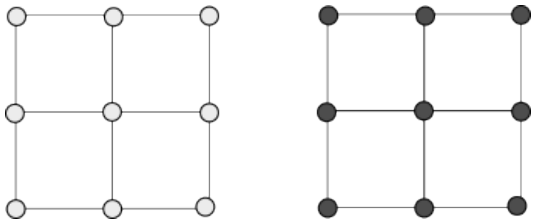
\includegraphics[width=0.4\linewidth]{Immagini/realizzazioni energia minima.png}
    \caption{realizzazioni corrispondenti ai microstati degeneri di energia minima.}
    \label{fig: realizzazioni energia minima}
\end{figure}
I termini successivi dello sviluppo sono via via più disordinati per l'introduzione di spin invertiti. Nel caso del reticolo quadrato in dimensione $D = 2$, l'inversione di uno spin, che può avvenire in qualsiasi degli $N$ siti, introduce quattro coppie di spin antiparallelo, come mostrato in figura \ref{fig: realizzazioni 1-flip e 2-flip}, per cui $\tilde{g}_1 = \tilde{g}_2 = \tilde{g}_3 = 0$ e $\tilde{g}_4 = N$. 
\begin{figure}[h]
    \centering
    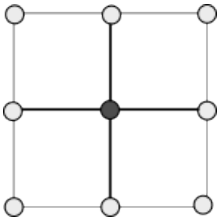
\includegraphics[width=0.2\linewidth]{Immagini/realizzazione 1-flip.png}
    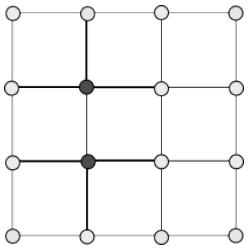
\includegraphics[width=0.2\linewidth]{Immagini/realizzazione 2-flip.png}
    \caption{realizzazione in seguito all'inversione dello spin di: (i) un sito; (ii) due siti.}
    \label{fig: realizzazioni 1-flip e 2-flip}
\end{figure}
Invece, non è possibile avere cinque coppie antiparallele, ma invertendo due spin primi vicini in uno degli $2N$ modi possibili diversi si possono ottenere sei coppie di spin antiparallelo, rappresentato sempre in figura \ref{fig: realizzazioni 1-flip e 2-flip}, insieme ovviamente alle configurazioni $\Z_2$ simmetriche rispetto a queste. Quindi, $\tilde{g}_5 = 0$, $\tilde{g}_6 = 2N$ e per questo particolare reticolo si ha
\begin{equation}
    \begin{split}
        Z &= 2e^{2NK}(1 + N\tilde{v}^4 + 2N\tilde{v}^6 + \cdots) \\
        &= 2e^{2NK}(1 + Ne^{-8K} + 2Ne^{-12K} + \cdots),\quad L = \frac{Nq}{2} = 2N.
    \end{split}
\end{equation}

\section{Argomento di Peierls}
La prima dimostrazione del fatto che il modello di Ising ammetta una fase ordinata in dimensione $D \ge 2$ è dovuta a Peierls. L'argomento di Peierls si applica nel limite termodinamico e permette di capire se ci si dovrebbe aspettare una transizione di fase o meno. Nel limite termodinamico, lo stato macroscopico del sistema all'equilibrio avrà energia libera $G$ minima. Una fase ordinata può esistere a patto che corrisponda ad un minimo stabile di $G$ rispetto alle fluttuazioni termiche, ovvero se queste ultime non abbassano l'energia libera. Quindi si deve vedere se le fluttuazioni termiche, in cui lo spin cambia di segno, alzano o abbassano l'energia libera rispetto alla configurazione ordinata. Ricapitolando, se $\Delta G \ge 0$, allora la fase è ordinata e $G$ permette un minimo stabile, al contrario se $\Delta G < 0$, allora il sistema è instabile.

\subsubsection{$\Delta G$ per il modello di Ising 1-dimensionale}
Partendo da uno stato completamente ordinato, mostrato in figura \ref{fig: variazione G D = 1}, si fissa un sito qualsiasi e ci si chiede se le fluttuazioni che portano a una configurazione in cui tale spin è invertito alzano o abbassano l'energia libera. 
\begin{figure}[h]
    \centering
    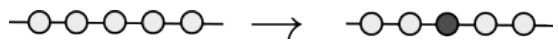
\includegraphics[width=0.5\linewidth]{Immagini/variazione G D = 1.png}
    \caption{inversione dello spin di un sito di un reticolo unidimensionale.}
    \label{fig: variazione G D = 1}
\end{figure}
La variazione di energia è $\Delta G=\Delta E-T\Delta S$. Nello stato iniziale l'energia è l'energia minima $E_0=-NJ$ (con condizioni periodiche perché ci sono $N$ link e sono tutti paralleli), mentre l'entropia è nulla in quanto c'è solo una configurazione possibile, per cui $S = k\log N_{\mathrm{config}} = k\log{1} = 0$.

Dato che alla variazione di energia $\Delta E$ contribuiscono solo i link che legano siti a spin antiparallelo, si ha una classe di configurazioni che corrispondono alla stessa $\Delta E$ dette ``isole di spin''. Le configurazioni in cui lo spin selezionato è invertito che hanno la minima variazione di energia sono quelle in cui si crea un'isola di spin invertiti, che comprende il sito scelto, come mostrato in figura \ref{fig: isola di spin D = 1}. Qualsiasi sia la lunghezza $L$ di tale isola, la variazione energetica rispetto allo stato ordinato è pari a
\begin{equation}
    \Delta E = 2 \times 2J = 4J
\end{equation}
perché si hanno ora due coppie contigue con spin antiparallelo per ciascuna delle quali il contributo all'energia è $J$ invece di $-J$.
\begin{figure}[h]
    \centering
    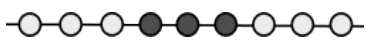
\includegraphics[width=0.35\linewidth]{Immagini/isola di spin D = 1.png}
    \caption{isola di spin in $D = 1$.}
    \label{fig: isola di spin D = 1}
\end{figure}

Vi sono $L$ modi di ``sistemare'' un'isola di lunghezza $L$ in modo che comprenda lo spin fissato\footnote{Ossia ci sono $L$ modi di sistemare il sito con spin invertito.}, per cui ora l'entropia non è nulla e si ha invece
\begin{equation}
    \Delta S = k \log L.
\end{equation}
Dunque, la variazione di energia libera è pari a 
\begin{equation}
    \Delta G = \Delta E - T \Delta S = 4J - kT \log L.
\end{equation}
Per qualsiasi $T>0$, si può trovare un valore di $L$ abbastanza grande da abbassare l'energia libera. Dunque, lo stato ordinato non è termodinamicamente stabile, per cui il modello unidimensionale non ammette una fase ordinata, come già dedotto dalla soluzione esatta, e non ci si aspetta una transizione di fase.

\subsubsection{$\Delta G$ per il modello di Ising 2-dimensionale}
Si consideri un'isola di spin invertiti che contenga un sito arbitrariamente scelto come fatto in figura \ref{fig: isola di spin D = 2}. 
\begin{figure}[h]
    \centering
    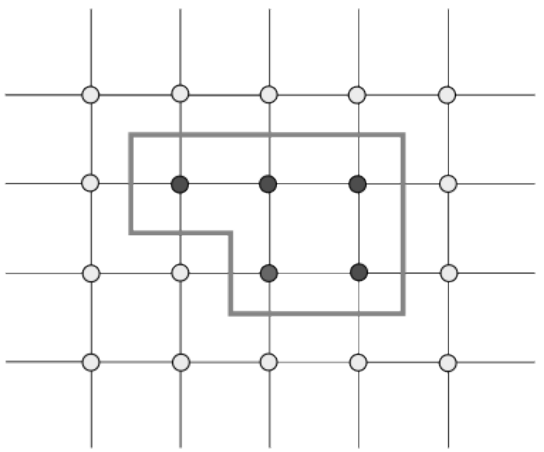
\includegraphics[width=0.35\linewidth]{Immagini/isola di spin D = 2.png}
    \caption{isola di spin in $D = 2$.}
    \label{fig: isola di spin D = 2}
\end{figure}
Si vogliono ora considerare tutte le fluttuazioni che invertono uno spin. Come prima cosa, si nota che il numero di coppie contigue con spin antiparallelo è pari al numero di link che attraversano il ``domain wall'' che racchiude l'isola. Introducendo quindi il reticolo duale, in cui vertici sono nel centro delle facce del reticolo originario, se il domain wall è un poligono fatto di $L$ segmenti (in figura \ref{fig: isola di spin D = 2} $L = 10$), nel reticolo duale essa è attraversata da $L$ links del reticolo originario, per cui
\begin{equation}
    \Delta E = 2JL,
\end{equation}
poiché si ha una variazione di $2J$ per ogni coppia con spin antiparallelo. Il numero di spin invertiti coincide con l'area $A(L)$ della regione circondata dal domain wall, cioè il numero di facce del reticolo duale contenute all'interno del domain wall. Non si conosce in generale il valore preciso dell'area, perché può avere forme diverse, ma sicuramente si può scrivere che
\begin{equation}
    A \le \bigg(\frac{L}{2\pi}\bigg)^2 \le \frac{L^2}{4\pi},
\end{equation}
in quanto deve essere minore o uguale alla figura con l'area maggiore, corrispondente ad un cerchio di raggio $L/2\pi$. Inoltre si possono avere diverse ``forme'' $\sigma(L)$ dell'isola, per le quali si può affermare che
\begin{equation}
    \sigma(L) \le 3^L,
\end{equation}
dato ad ogni ``passo'' ci si può muovere in tre direzioni; tuttavia, questa è una stima superiore perché non tutte le scelte sono libere, dato che la curva deve chiudersi. In definitiva, il numero di configurazioni $W(L)$, che consiste in isole di spin invertiti che creano $L$ coppie di spin antiparallelo è dato da
\begin{equation}
    W(L) \le 3^L\frac{L^2}{4\pi},
\end{equation}
da cui si ricava che la variazione di entropia è
\begin{equation}
    \Delta S = k\log{W(L)} \le kL\ln3 + \mathcal{O}(\log{L}),
\end{equation}
per cui la variazione di energia libera risulta essere
\begin{equation}
    \Delta G = \Delta E - T\Delta S \ge (2JL - kT\log{3})L - \mathcal{O}(\log{L}).
\end{equation}
Dunque, si ha una competizione fra il termine energetico e quello entropico, poiché entrambi scalano con $L$. Fissato l'accoppiamento $J$ per $kT$ sufficientemente piccolo, se si prova ad invertire degli spin e creare delle fluttuazioni, queste risultano sfavorite anche da un punto di vista dell'energia libera, e non solo da un punto di vista dell'energia interna $E$. Si ha sempre $\Delta G \ge 0$, cioè lo stato ordinato è stabile e si ha una fase ordinata a bassa temperatura. Quindi, si era visto che esiste una fase disordinata ad alte temperature, mentre ora si è visto che esiste fase ordinata a basse temperature, pertanto deve esistere una transizione di fase di mezzo. Conclusioni analoghe si traggono per $D > 2$.

\section{Dualità di Kramers - Wannier}
Si ricorda che nello sviluppo ad alta temperatura si era indicato con $g_l$ il numero di poligoni chiusi di lunghezza $l$, mentre nello sviluppo a bassa temperatura si era indicato con $\tilde{g}_l$ il numero di link che univano due siti con spin antiparallelo. Nel caso del reticolo quadrato in $D = 2$ è immediato notare che 
\begin{equation}
    g_l = \tilde{g}_l,
\end{equation}
dato che ogni poligono chiuso in un reticolo può essere associato tramite una corrispondenza uno ad uno con un ``domain wall'' nel reticolo duale, come mostrato in figura \ref{fig: dualità KW D = 2}. Sfruttando questa corrispondenza, si può collegare l'espansione ad alta temperatura con un dato valore di $K$, e quindi di $v$, con l'espansione a bassa temperatura per questo particolare reticolo, le quali sono date rispettivamente da
\begin{align}
    Z(K) &= (2\cosh^2{K})^N\sum_{l=0}^Lg_lv^l, \\
    Z(\tilde{K}) &= 2e^{2\tilde{K}N}\sum_{l=0}^Lg_l\tilde{v}^l,
\end{align}
dove si è introdotto il parametro duale $\tilde{K}$.
\begin{figure}[h]
    \centering
    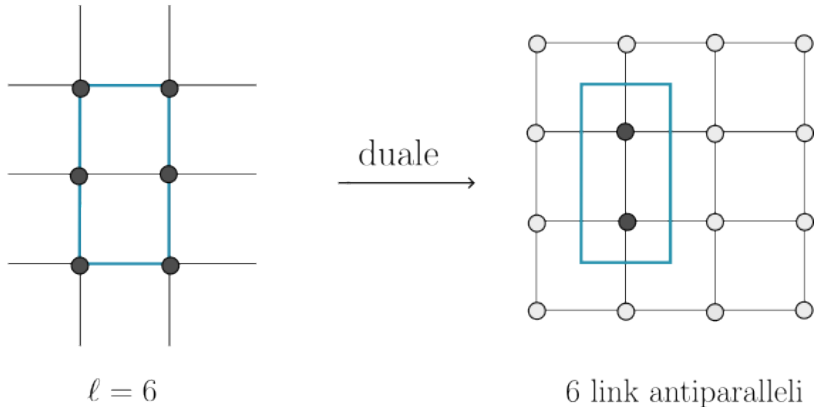
\includegraphics[width=0.53\linewidth]{Immagini/dualità KW D = 2.png}
    \caption{corrispondenza tra un poligono chiuso e il domain wall duale.}
    \label{fig: dualità KW D = 2}
\end{figure}

Inoltre, si nota che le serie in questione sono le medesime ma con diversa ragione; ci si chiede quindi se sia possibile connettere le due espressioni. Per farlo, si deve richiedere che $v = \tilde{v}$, ovvero che $e^{-2\tilde{K}} = \tanh{K}$, da cui si ricava la mappa di dualità
\begin{equation}
\label{eq: mappa di dualità}
    \tilde{K} = -\frac{1}{2}\log\tanh{K}\Longleftrightarrow \sinh{2\tilde{K}} = \frac{1}{\sinh{2K}},
\end{equation}
dove la seconda espressione mostra chiaramente come la mappa associ piccoli valori di $K$ a grandi valori di $\tilde{K}$.
\begin{obs}
    Si nota che se si applica due volte la mappa \eqref{eq: mappa di dualità} si torna al punto di partenza, infatti
    \begin{equation}
        K \longrightarrow \tilde{K} \longrightarrow \tilde{\tilde{K}} \equiv K.
    \end{equation}
\end{obs}
Avendo imposto che $v = \tilde{v}$, l'espansione ad alta temperatura \eqref{eq: funzione di partizione Ising alta T} può essere riscritta come
\begin{equation}
    Z(K) = [2\cosh^2{(K)}e^{-2\tilde{K}}]^Ne^{2\tilde{K}N}\sum_{l=0}^Lg_lv^l = [2\cosh^2{(K)}\tanh{(K)}]^N\frac{Z(\tilde{K})}{2},
\end{equation}
da cui, sfruttando le relazioni trigonometriche iperboliche, si arriva infine alla relazione di dualità di Kramers - Wannier
\begin{equation}
\label{eq: relazione Kramers-Wannier}
    Z(K) = \frac{1}{2}(\sinh{2K})^NZ(\tilde{K}).
\end{equation}
Questa relazione permette di determinare subito un'espansione se si è già calcolata la sua duale. Tuttavia, si deve notare che vale unicamente nel limite termodinamico in cui gli effetti delle condizioni al contorno sono trascurabili. Se questo non è il caso, allora bisogna tenere conto che sotto la trasformazione di dualità le condizioni al contorno per $Z(K)$ cambiano e la relazione di dualità diventa più complessa. Ad ogni modo, la relazione \eqref{eq: relazione Kramers-Wannier} implica per l'energia libera $G$ che
\begin{equation}
\label{eq: relazione Kramers-Wannier energia libera}
    \begin{split}
        G(K) &= -\frac{1}{\beta}[\log{Z(\tilde{K})} + N\log{(\sinh{2K})} - \log{2}] \\
        &= G(\tilde{K}) - \frac{N}{\beta}\log{(\sinh{2K})} + \frac{\log{2}}{\beta}.
    \end{split}
\end{equation}

\subsubsection{Temperatura critica}
La dualità di Kramers - Wannier permette di determinare in modo esatto il valore della temperatura critica $T_c$ a cui avviene la transizione ferromagnetica nel modello di Ising bidimensionale su reticolo quadrato. Siccome i termini ``aggiuntivi'' nel membro di destra della relazione di dualità \eqref{eq: relazione Kramers-Wannier energia libera} non hanno singolarità per $T > 0$, le singolarità di $G(K)$ sono mappate uno ad uno nelle singolarità di $G(\tilde{K})$, quindi $0 < K_c < K$. In generale, se ci si trova in una certa fase e se c'è una transizione di fase, ci sarà un certo punto critico $K_c$ che corrisponderà alla singolarità della funzione $G(K)$. La zona corrispondente a valori grandi di $K$, sarà quella di bassa temperatura, quindi $\tilde{K} < \tilde{K}_c < 0 $, dove valori grandi $\tilde{K}$ corrispondono a valori piccoli $K$ e viceversa. Essendoci un solo punto di singolarità ed una sola funzione $G$ si deve per forza avere
\begin{equation}
    K_c = \tilde{K}_c.
\end{equation}
Dunque, il valore critico è quello invariante per dualità. Dalla struttura del modello, dall'intuizione fisica e dall'argomento di Peierls si può assumere che vi sia un solo punto di transizione di fase: quello della transizione ferromagnetica ordine-disordine. Sotto la mappa di dualità, l'equazione \eqref{eq: mappa di dualità} implica che
\begin{equation}
    \sinh{(2K)}\sinh{(2\tilde{K})} = 1,
\end{equation}
da cui, per $K_c = \tilde{K}_c$, si trova la relazione
\begin{equation}
\label{eq: relazione per K critico}
    \begin{split}
        \sinh^2{2K_c} = 1&\quad\Longrightarrow\quad \sinh{2K_c} = \frac{e^{2K_c} - e^{-2K_c}}{2} = 1\\
        &\quad\Longrightarrow\quad e^{2K_c} = 1 + \sqrt{2}
    \end{split}
\end{equation}
che determina esattamente $K_c$ come
\begin{equation}
\label{eq: K critico}
    K_c = \frac{J}{kT_c} = \frac{1}{2}\log{(1 + \sqrt{2})} \simeq 0.44,
\end{equation}
o equivalentemente 
\begin{equation}
    kT_c = \frac{2J}{\log{(1 + \sqrt{2})}} \simeq \SI{2.27}{\joule}.
\end{equation}

\section{Soluzione di Onsager}
La prima derivazione esatta della funzione di partizione del modello di Ising bidimensionale, a campo magnetico esterno nullo è dovuta ad Onsager sfruttando il metodo della matrice di trasferimento, passando dal caso $d=1$ a quello $d=2$. Nel caso $d=1$ si aveva una catena di spin, come quella in figura \ref{fig: soluzione Onsager D = 1}, e la funzione di partizione era
\begin{equation}
    Z \propto \Tr{\TM}^N, \quad\TM\in\R^{2,2}
\end{equation}
in cui la matrice di trasferimento lega i possibili valori di $s_i$ a quelli del sito successivo $s_{i+1}$.
\begin{figure}[h]
    \centering
    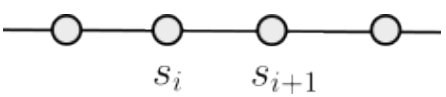
\includegraphics[width=0.35\linewidth]{Immagini/soluzione Onsager D = 1.png}
    \caption{catena di spin in $D = 1$.}
    \label{fig: soluzione Onsager D = 1}
\end{figure}

Onsager fa un discorso simile in $D = 2$. Si immagini di avere un reticolo quadrato con $N = M^2$ siti e di organizzarlo in $M$ righe e $M$ colonne, come mostrato in figura \ref{fig: soluzione Onsager D = 2}. Quindi, al posto di collegare $s_i$ ed $s_{i+1}$, la matrice di trasferimento lega i possibili valori della riga $M_i$ con i possibili valori della riga successiva $M_{i+1}$. La collezione di spin $s_A$ che descrive la configurazione di una certa riga, è una collezione del tipo
\begin{equation}
    s_A = \{ s_1^{i}, s_2^{i}, \dots, s_N^{i} \}.
\end{equation}
Data una collezione di spin che hanno valori $s_A = \pm 1$, questi oggetti corrispondono ai pesi della rappresentazione spinoriale del gruppo delle rotazioni. Questi spin possono avere $2^M$ indici, quindi la matrice $T$ è in generale una matrice di dimensione $(2^M \times 2^M)$. 
\begin{figure}[h]
    \centering
    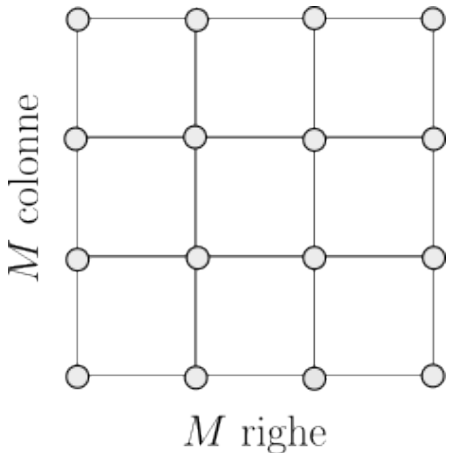
\includegraphics[width=0.3\linewidth]{Immagini/soluzione Onsager D = 2.png}
    \caption{reticolo quadrato di $N = M^2$ siti in $D = 2$.}
    \label{fig: soluzione Onsager D = 2}
\end{figure}
Quindi, già solo passando da $D = 1$ a $D = 2$ si va incontro ad una grande complicazione algebrica: lo spazio stesso della matrice tende a divergere nel limite termodinamico. Sfruttando le proprietà algebriche è possibile, anche se non è semplice, mostrare che
\begin{equation}
    Z = (2\cosh{K}e^I)^N,\quad I = \int_0^{\pi} \frac{d\phi}{2\pi} \, \log{\bigg(\frac{1 + \sqrt{1 - \kappa^2 \sin^2 \phi}}{2}\bigg)}
\end{equation}
con
\begin{equation}
    \kappa = \frac{2 \sinh(2K)}{\cosh^2(2K)} = \frac{2 \sinh(2K)}{1 + \sinh^2(2K)}.
\end{equation}
L'energia libera $G = -\log{(Z)}/\beta$ vale quindi
\begin{equation}
\label{eq: energia libera Onsager}
    G = -\frac{N}{\beta} \log(2 \cosh K) - \frac{N}{\beta} I .
\end{equation}
Per via del contributo $NI/\beta$, si ha un punto di non-analiticità legato al ``branching point'' della radice quadrata, quando
\begin{equation}
    \begin{split}
        \kappa = \kappa_c = 1 &\quad\Longleftrightarrow\quad \sinh^2(2K_c) - 2 \sinh(2K_c) + 1 = 0 \\
        &\quad\Longleftrightarrow\quad [\sinh(2K_c) - 1]^2 = 0 \\
        &\quad\Longleftrightarrow\quad \sinh(2K_c) = 1,
    \end{split}
\end{equation}
che è la stessa determinazione ottenuta dalla dualità di Kramers - Wannier nell'equazione \eqref{eq: relazione per K critico} che determina il valore critico, già trovato nella \eqref{eq: K critico}, come
\begin{equation}
    K_c = \frac{1}{2} \log(1 + \sqrt{2}) \simeq 0.44.
\end{equation}
In altre parole, $K_c$ è il punto in cui $G$ o le sue derivate possono sviluppare un comportamento singolare. In realtà, come deve essere, l'energia libera $G$ è regolare nel punto critico, infatti da $G(T,N,h = 0)$ si possono ricavare
\begin{equation}
    S = -\frac{\p G}{\p T}\bigg|_N,
    \quad
    E = -\frac{\p \log Z}{\p \beta}\bigg|_N
      = \frac{\p}{\p \beta}(\beta G)\bigg|_N.
\end{equation}
A partire dall'espressione \eqref{eq: energia libera Onsager} per $G$ si possono ricavare le espressioni esatte in termini di integrali ellittici di modulo $\kappa$, che risultano ancora continue nel punto di transizione $\kappa = \kappa_c = 1$. Quindi, per l'energia interna, per l'entropia e per l'energia libera, si trovano delle espressioni continue nel punto critico. Il fatto che ci sia questa continuità indica che se c'è una transizione di fase, questa deve essere del secondo ordine, senza calore latente. Dunque, la singolarità si deve presentare nell'espressione della capacità termica. Nel caso in cui $h = 0$, si può calcolare esattamente anche il calore specifico 
\begin{equation}
    c_N = \frac{\p E}{\p T} \bigg|_N,
\end{equation}
che risulta di nuovo espresso in termini di integrali ellittici, ma in modo tale da presentare una singolarità logaritmica per $K \to K_c$, cioè per $T \to T_c$. Si trova quindi che 
\begin{equation}
    c_N \propto kN\log{|t|},\quad t = \frac{T - T_c}{T_c}.
\end{equation}
L'andamento del calore specifico nei pressi del punto critico è logaritmico, quindi l'indice critico $\alpha$ introdotto nella \eqref{eq: legge di potenza suscettività e calore specifico} risulta essere pari a $\alpha_{\mathrm{exact}} = 0$. Infine, l'andamento del calore specifico è quello mostrato in figura \ref{fig: andamento cap. termica e M (Ising)}, in cui il calore specifico diverge avvicinandosi al punto critico.

L'espressione dell'energia libera nel caso in cui $h = 0$ non è invece sufficiente per derivare l'espressione della magnetizzazione
\begin{equation}
    M = -\frac{\p G}{\p h} \bigg|_{T,N}.
\end{equation}
Quindi, si dovrebbe accendere il campo magnetico almeno al primo ordine, fare la derivata e poi porlo uguale a zero. Risulta così ancora possibile ottenere il risultato esatto, annunciato prima da Onsager e derivato poi in dettaglio da Yang, dato da
\begin{equation}
    M(T,N,h = 0) =
    \begin{cases}
        N \bigg( 1 - \dfrac{1}{\sinh^2 2K} \bigg)^{1/8},\quad T < T_c \\[2ex]
        0,\quad T \ge T_c
    \end{cases},
\end{equation}
da cui si deduce che l'andamento della magnetizzazione ha la forma mostrata in figura \ref{fig: andamento cap. termica e M (Ising)}. Ovviamente, per la simmetria $\Z_2$ c'è anche la possibilità che si sviluppi al di sotto di $T_c$ la magnetizzazione opposta in segno. Vicino al punto critico, dalla precedente espressione segue, con $T < T_c$ (ossia per $t < 0$), che 
\begin{equation}
    M \simeq 1.22 \times N (-t)^{1/8}.
\end{equation}
Quindi, il valore esatto dell'esponente critico $\beta$ introdotto nell'equazione \eqref{eq: legge di potenza magnetizzazione}, in assenza di campo esterno, è pari a 
\begin{equation}
    \beta_{\mathrm{exact}} = \frac{1}{8}.
\end{equation}
Invece, il calcolo della suscettività magnetica è più complesso, tralasciando i dettagli matematici si trova che vicino al punto critico l'andamento della suscettività è della forma
\begin{equation}
    \chi \simeq |t|^{-7/4}.
\end{equation}
Dunque, il valore esatto dell'indice critico $\gamma$ introdotto nella \eqref{eq: legge di potenza suscettività e calore specifico} è pari a 
\begin{equation}
    \gamma_{\mathrm{exact}} = \frac{7}{4}.
\end{equation}
\begin{figure}[h]
    \centering
    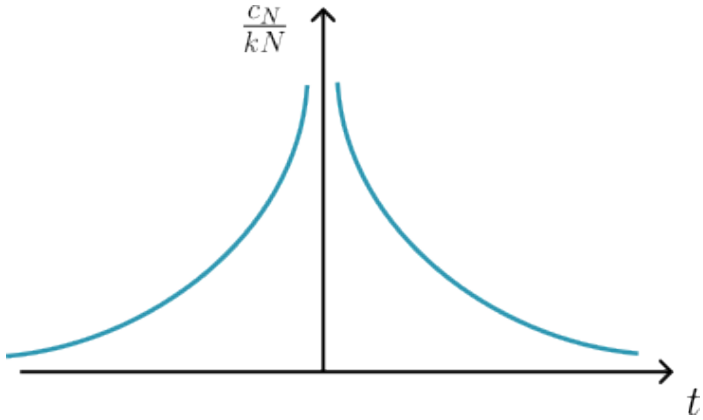
\includegraphics[width=0.4\linewidth]{Immagini/andamento cap. termica (Ising).png}
    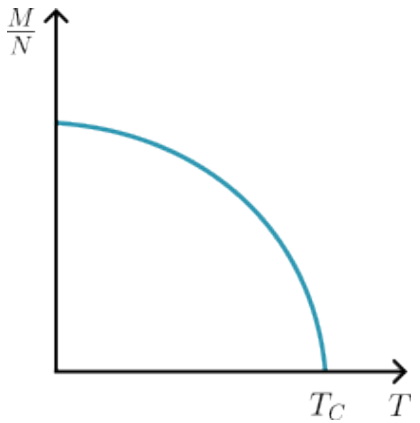
\includegraphics[width=0.3\linewidth]{Immagini/andamento M (Ising).png}
    \caption{andamento per il modello di Ising in $D = 2$ di: (i) $c_N/kN$ in funzione di $t$; $M/N$ in funzione di $T$.}
    \label{fig: andamento cap. termica e M (Ising)}
\end{figure}

\section{Correlatori}
I correlatori sono un tipo di osservabile che contengono informazioni sul modello e sul suo comportamento ai punti critici. Queste informazioni sono codificate nelle funzioni di correlazione tra spin in siti diversi e permettono di capire quanto questi si influenzino. Si consideri il correlatore
\begin{equation}
    \vmedio{s_is_j},
\end{equation}
dove $i$ e $j$ sono siti posti a distanza $r$ espressa in unità del passo reticolare. Per $r \to \infty$, i due spin non si possono influenzare e il correlatore si fattorizza secondo la ``cluster decomposition'' come
\begin{equation}
    \vmedio{s_i s_j} \underset{r \to \infty}{\longrightarrow} \vmedio{s_i}\vmedio{s_j}.
\end{equation}
Quindi, conviene introdurre il correlatore connesso $G_{ij}$ come
\begin{equation}
    G_{ij} := \vmedio{s_i - s_j}_c = \vmedio{s_is_j} - \vmedio{s_i}\vmedio{s_j}.
\end{equation}
Per un reticolo infinito o con condizioni al contorno periodiche, il valore del correlatore può solo dipendere dalla distanza relativa, per cui non dipende da dove sono posizionati i due spin. Di conseguenza, si presenta un'invarianza per traslazioni e $G_{ij}$ dipende solo dalla posizione relativa di $i$ e $j$. 

Il correlatore $G_{ij}$ si può ottenere introducendo un campo magnetico variabile da sito a sito $h_m$ in modo che
\begin{equation}
    j_m = \beta h_m
\end{equation}
giochi il ruolo di ``sorgente'' dato che si accoppia linearmente ad ogni spin, in modo analogo alla sorgente $j(x)$ che viene introdotta in Teoria dei campi. La funzione di partizione quindi è
\begin{equation}
    Z(j) = \sum_{\{s_i\}} e^{-\beta H + \sum_k j_k s_k},
\end{equation}
così che $Z(j=0)$ sia l'usuale funzione di partizione del modello di Ising a campo nullo \eqref{eq: funzione di partizione Ising D=1}. Per semplicità, si pone $j \cdot s \equiv \sum_k j_k s_k$, quindi si calcola
\begin{equation}
    \frac{\p}{\p j_n} \log Z(j)
    = \frac{1}{Z} \frac{\p}{\p j_n} \sum_{\{s_i\}} e^{-\beta H + j \cdot s}
    = \frac{1}{Z} \sum_{\{s_i\}} s_n e^{-\beta H + j \cdot s}
    \equiv \vmedio{s_n}_j,
\end{equation}
dove $\vmedio{s_n}_j$ indica il valore di aspettazione in presenza del termine di sorgente. Derivando una seconda volta si ottiene
\begin{equation}
    \begin{split}
        \frac{\p^2}{\p j_m \p j_n} \log Z(j)
        &= \frac{1}{Z} \sum_{\{s_i\}} s_m s_n e^{-\beta H + j \cdot s} - \frac{1}{Z^2}\bigg(\frac{\p}{\p j_m}Z\bigg)\sum_{\{s_i\}} s_n e^{-\beta H + j \cdot s} \\
        &= \vmedio{s_m s_n}_j - \frac{\p}{\p j_m}\log{(Z\vmedio{s_n}_i)} \\
        &= \vmedio{s_m s_n}_j - \vmedio{s_m}_j\cdot\vmedio{s_n}_j \\
        &= \vmedio{s_ms_n}_c.
    \end{split}
\end{equation}
Quindi, il correlatore connesso $G_{mn}$ nel modello di Ising a campo esterno nullo è dato da
\begin{equation}
    G_{mn} = \vmedio{s_m s_n}_c|_{j = 0} = \frac{\p^2}{\p j_m \p j_n} \log Z(j) \bigg|_{j=0},
\end{equation}
che corrisponde a dire che $\log{Z(j)}$ è la funzione generatrice dei correlatori connessi. Questa relazione si generalizza a funzioni di correlazione tra più spin, in perfetta analogia con la Teoria dei campi. Si nota anche come la derivazione precedente mostri che
\begin{equation}
    G_{mn} = \frac{\p}{\p j_m} \vmedio{s_n}_j \bigg|_{j=0},
\end{equation}
ossia il correlatore rappresenta la risposta del valore medio dello spin nel sito $n$ alla variazione del campo magnetico $h_m = j_m / \beta$ nel sito $m$. Questo perché in sostanza il fatto che ci sia una variazione di campo magnetico nel sito $m$ determina il cambiamento del valore medio in $n$ e il correlatore descrive come questo avviene.

\subsubsection{Correlatore in dimensione $D$ generica}
Si può dare un'espressione del correlatore diretto anche in termini del modello di Ising con $h = 0$ nell'espansione ad alta temperatura. In questo caso, $T > 0$ e si è nella fase disordinata in cui la simmetria non viene rotta e dove non si ha magnetizzazione spontanea, per cui $\vmedio{s_k} = 0$. Dunque, il correlatore è dato da
\begin{equation}
\label{eq: correlatore Ising D-dimensionale}
    G_{kn} = \vmedio{s_k s_n} = \sum_{\{s_i\}} s_k s_n \frac{\exp{(K\sum_{\vmedio{ij}}s_is_j)}}{Z},
\end{equation}
che nel limite ad alta temperatura, usando l'identità \eqref{eq: relazione exp(Ksisj) e cosh(K)}, diventa
\begin{equation}
    G_{kn} = \frac{1}{Z}\sum_{\{s_i\}} s_ks_n\prod_{\vmedio{ij}}[\cosh{(K)}(1 + s_is_jv)].
\end{equation}
Si vede che, con gli stessi ragionamenti fatti per derivare la funzione di partizione $Z$, che i contributi interessanti sono solo quelli corrispondenti alle possibili catene di link attivi che collegano i siti $k$ e $n$, moltiplicati per i possibili cammini chiusi. Un tipico contributo sarà della forma mostrata in figura \ref{fig: contributo correlatore D generica (alta T)}, quindi si avrà una linea che congiunge $s_k$ con $s_n$ più le possibili traiettorie chiuse, come il quadratino in alto a sinistra.
\begin{figure}[h]
    \centering
    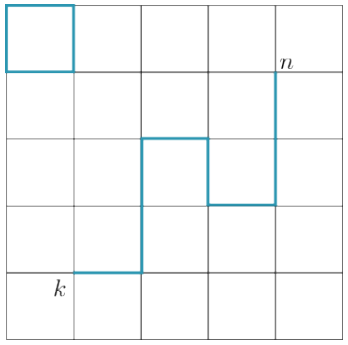
\includegraphics[width=0.3\linewidth]{Immagini/contributo correlatore D generica (alta T).png}
    \caption{contributo tipico del correlatore $G_{kn}$ nel limite di alta temperatura in $D$ generica.}
    \label{fig: contributo correlatore D generica (alta T)}
\end{figure}
I cammini chiusi, che si fattorizzano, sono gli stessi diagrammi che compaiono nella funzione di partizione. Insieme con i fattori globali $2^N(\cosh{K})^L$ si cancellano
con il fattore $Z$ a denominatore nella \eqref{eq: correlatore Ising D-dimensionale}. In definitiva il correlatore si organizza con un'espansione di potenze di $v$ data da
\begin{equation}
\label{eq: correlatore Ising D-dimensionale (espansione in serie)}
    G_{kn} = \nsum_l g_l^{(k,n)}v^l,
\end{equation}
dove il coefficiente $g_l^{(k,n)}$ è il numero di percorsi di lunghezza $l$ che congiungono i siti $k$ ed $n$. Se si ha invarianza per traslazione, tale numero dipende solo dalla posizione relativa di $k$ ed $n$, in forte analogia con il propagatore in Teoria dei campi $G(x,y) = \mybraket{\Phi(x)}{\Phi(y)}$. L'espressione \eqref{eq: correlatore Ising D-dimensionale (espansione in serie)} in traiettorie pesate da $v^l$, il quale dipende dalla lunghezza della traiettoria stessa, corrisponde alla realizzazione di $G(x,y)$ come ``path integral'' sulle traiettorie che congiungono $x$ ed $y$ pesate dal fattore $e^{-S[d]}$.

\subsubsection{Correlatore in dimensione $D = 1$}
Si studia adesso il caso 1-dimensionale. Anche qui ci si trova sempre nella fase disordinata nel limite di alta temperatura. 
\begin{figure}[h]
    \centering
    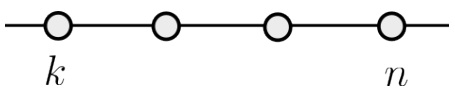
\includegraphics[width=0.3\linewidth]{Immagini/contributo correlatore D = 1 (alta T).png}
    \caption{l'unico contributo del correlatore $G_{kn}$ nel limite di alta temperatura in $D = 1$}
    \label{fig: contributo correlatore D = 1 (alta T)}
\end{figure}
In questo caso, la possibile traiettoria da $k$ ad $n$ è solamente una, mostrata in figura \ref{fig: contributo correlatore D = 1 (alta T)}, e la distanza in passo reticolare è $l = |n-k|$, quindi il correlatore è
\begin{equation}
    G_{kn} = \vmedio{s_k s_n} = \sum_{\{s_i\}} s_k s_n \frac{\exp{(K \sum_l s_l s_{l+1}})}{Z},
\end{equation}
da cui, utilizzando lo sviluppo ad alte temperature \eqref{eq: identità sviluppo alta T}, si vede come la somma sui valori di $s_i$ in qualsiasi sito richieda un numero pari di variabili $s_i$ per non annullarsi, per cui l'unico contributo non nullo è quello di una catena di link attivi dal sito $k$ al sito $n$ che fornisce
\begin{equation}
    G_{kn} = \frac{2^N \cosh^L K (\tanh K)^{|n-k|}}{2^N \cosh^L K} = (\tanh K)^{|n-k|}.
\end{equation}
Inoltre, si nota che il correlatore ha un andamento esponenziale che in particolare decresce con la distanza; quindi, si può riscrivere l'espressione del correlatore come
\begin{equation}
    G_{kn} = e^{-|n-k|/\xi},\quad \xi = \bigg(\log \frac{1}{\tanh{K}}\bigg)^{-1} > 0,
\end{equation}
dove $\xi$ rappresenta la lunghezza di correlazione e non diverge per alcuna $T > 0$.

\section{Teorema fluttuazione - risposta}
Si intende ora studiare la relazione che intercorre tra la suscettività magnetica e l'ampiezza delle fluttuazioni della magnetizzazione, dovute alla presenza di un campo esterno. Si consideri la magnetizzazione $M$ definita come nella \eqref{eq: magnetizzazione come media spin}. Se la dimensione del reticolo e/o le condizioni al contorno permettono di assumere l'invarianza per traslazioni del sistema, allora gli $s_n$ sono tutti uguali e $\vmedio{s_n}$ non dipende dallo specifico valore di $n$, che si può fissare ad esempio a $n = 1$, per cui 
\begin{equation}
    M = N \vmedio{s_1} = Nm,
\end{equation}
dove $m$ è la magnetizzazione del singolo sito. Si supponga ora di ``accendere'' un campo esterno costante $h$ (che non pregiudica l'invarianza per traslazioni essendo costante sui siti) e si calcoli la suscettività magnetica
\begin{equation}
    \chi = \frac{\p M}{\p B} = \mu_B \frac{\p M}{\p h} = N \mu_B \frac{\p \vmedio{s_1}}{\p h},
\end{equation}
dalla quale si deduce che $\vmedio{s_1}$ risponde, tramite il correlatore $G_{mn}$, alla variazione del campo esterno in ogni altro sito $n$. Per il campo costante $h$, che è uguale in tutti i siti, si ha
\begin{equation}
    h_n = \frac{j_n}{\beta} \equiv h,\quad \forall n,
\end{equation}
ossia c'è una sorgente in ognuno degli altri siti. Quindi, si vuole capire come cambia il valore di aspettazione di un qualsiasi spin, per esempio $s_1$, quando cambia il campo $h$. In sostanza, si sceglie uno spin e si va a vedere la somma dei suoi correlatori con tutti gli altri spin. Ad ogni modo, la suscettività adesso è
\begin{equation}
    \chi = N \mu_B \beta \nsum_n\frac{\p \vmedio{s_1}}{\p j_n} \bigg|_{h_n = h} = N \mu_B \beta \nsum_n G_{1n}.
\end{equation}
 Per la definizione di correlatore connesso, $G_{1n}$ è sostanzialmente diverso da zero solo se gli spin $s_1$ e $s_n$ sono correlati. Dunque, $\sum_n G_{1n} \propto \chi$ conta il numero di spin correlati con lo spin $s_1$ e, per invarianza sotto traslazioni, con qualsiasi altro spin ed è pertanto legato al range di correlazione nel sistema. Infatti, quando la suscettività $\chi$ diverge, questo segnala l'emergere di correlazione a lungo raggio nel sistema. Questo è anche legato alla divergenza della dimensione delle fluttuazioni della magnetizzazione. Infatti, valendo l'invarianza per traslazioni, $G_{kn}$ dipende solo dalla posizione relativa di $k$ e $n$, per cui
\begin{equation}
    N \nsum_n G_{1n} = \nsum_{k,n} G_{kn},
\end{equation}
ma d'altro canto si ha
\begin{equation}
    \begin{split}
        \sum_{k,n} G_{kn} = \sum_{k,n} \vmedio{s_k s_n} - \sum_{k,n} \vmedio{s_k} \vmedio{s_n} &= \bigvmedio{\left( \nsum_n s_n \right)^2} - \bigvmedio{\nsum_n s_n}^2 \\
        &= \vmedio{M^2} - \vmedio{M}^2 \\
        &\equiv\sigma_M^2.
    \end{split}
\end{equation}
Dunque, la suscettività si può scrivere come
\begin{equation}
\label{eq: relazione suscettività - magnetizzazione}
    \chi = \frac{\mu_B}{kT}\sum_{k,n}G_{kn} = \frac{\mu_B}{kT}\sigma_M^2.
\end{equation}
Questa relazione rappresenta un'istanza del teorema di fluttuazione - risposta: 
\begin{quote}
    ``la risposta del sistema ad una variazione del campo esterno $B$, codificata dalla suscettività magnetica $\chi$, è collegata all'ampiezza delle fluttuazioni della magnetizzazione espressa dalla varianza di tale quantità''.
\end{quote}
Si nota inoltre che la precedente relazione assicura che $\chi > 0$. Tuttavia, è anche da osservare come quest'ultima sia stata derivata considerando la presenza di un campo esterno $B$, così da poter effettuare la derivata e determinare $\chi$, ma resta vera se, dopo aver svolto la derivata, si pone $B = 0$. Dunque, nel caso di campo esterno nullo, le fluttuazioni della magnetizzazione spontanea  sono legate alla risposta del sistema all'accensione di un campo esterno.

\subsection{Comportamento intorno al punto critico}
La relazione fluttuazione-risposta aiuta a delineare un'immagine qualitativa del comportamento del sistema vicino al punto di transizione di fase. La suscettività magnetica diverge con un certo esponente critico $\chi \propto |t|^{-\gamma}$; ad esempio, nel modello di Ising 2-dimensionale a campo nullo, si era visto che visto che $\gamma_{\mathrm{exact}} = 7/4$. L'equazione \eqref{eq: relazione suscettività - magnetizzazione} implica allora che l'ampiezza delle fluttuazioni della magnetizzazione diverge anch'essa avvicinandosi al punto critico. Si parte ora dalla fase ordinata, per $T < T_c$, e si suppone che la magnetizzazione sia positiva, ossia $M > 0$. Le configurazioni tipiche, cioè quelle che pesano nel determinare le osservabili, sono isole di spin con spin pari $-1$ in un mare di spin pari a $+1$. La dimensione media di queste isole rappresenta la lunghezza di correlazione $\xi$ del sistema e fornisce una scala in termini della quale misurare le distanze. Andando verso il punto critico, la suscettività $\chi$ diverge e con essa diverge ad infinito la lunghezza di correlazione $\xi$. Questa divergenza è caratterizzata da un altro esponente critico del sistema con
\begin{equation}
    \xi \propto |t|^{-\nu}.
\end{equation}
Le fluttuazioni della magnetizzazione divergono, il che significa che diventano rilevanti le configurazioni con isole di tutte le dimensioni. Non c'è più una scala tipica, finita, del sistema, che appare simile a qualsiasi scala sia osservata (come un frattale). Il sistema diventa invariante per trasformazioni di scala. Siccome non vi è alcuna scala privilegiata che domina il sistema, i parametri microscopici del modello usato (il tipo di reticolo, valore di $J$, ...) non possono giocare alcun ruolo nella descrizione del sistema nelle vicinanze del punto critico. Quindi, le proprietà critiche del sistema dipendono solo da caratteristiche molto generali quali la dimensionalità $D$, il gruppo di simmetria che si rompe nella transizione, e così via. Queste sono codificate da un set di indici, o di ``esponenti'', critici $\alpha$, $\beta$ e $\gamma$ che individuano classi di universalità di sistemi, tra di loro anche molto diversi microscopicamente, accomunati dallo stesso comportamento critico. Ricapitolando, quando ci si avvicina al punto critico di transizione di fase, c'è una divergenza della lunghezza di correlazione, per cui ogni spin sente tutti gli altri e si perde la scala tipica del sistema. Questo significa che, vicino al punto critico, i dettagli non contano più, ma si vedono solo delle quantità che si comportano seguendo certe leggi di potenza e si parla di classi di universalità.

\section{Approssimazione di campo medio}
Fino ad ora non si è descritto alcun approccio che riesca a determinare il comportamento del modello di Ising per $D > 1$ in presenza di campo magnetico esterno. Un possibile, approccio è quello di tipo numerico basato sulle simulazioni di Montecarlo. Invece, un approccio analitico, basato però su forti approssimazioni, è quello del ``campo medio'', applicabile a molti modelli diversi. Per il modello di Ising, fornisce risultati tanto più corretti quanto più è alta la dimensione del reticolo, mentre per dimensioni basse questo approccio fornisce risultati solo qualitativamente validi. Anche se prevede la transizione di fase ferromagnetica, ma il set di indici critici differisce parecchio da quelli della soluzione esatta nel caso in cui $h = 0$ in $D = 2$ e da quelli forniti da accurate simulazioni numeriche. In $D = 1$ poi, anche qualitativamente si ha un disaccordo, poiché il campo medio continua a prevedere un punto di transizione del secondo ordine, mentre la soluzione esatta mostra che esso non è presente. L'approssimazione di campo medio consiste nel trascurare le fluttuazioni della magnetizzazione, o meglio nel considerarle solo all'ordine lineare. Questo è equivalente a focalizzarsi su un singolo spin $s_i$ in un qualsiasi sito $i$ e congelare tutti gli altri al loro valore medio
\begin{equation}
    \vmedio{s_k} = m = \frac{M}{N}.
\end{equation}
Pertanto, si ha una sola variabile dinamica $s_i$ che interagisce con i primi vicini, dove lo spin vale $m$. Essenzialmente, si sta dicendo che la dinamica avviene perché gli spin potrebbero cambiare, ma uno per volta. Nella pratica, si hanno solo due configurazioni che se $ h = 0$ sono come quelle mostrate in figura \ref{fig: realizzazioni ACM}, con $s_i = \pm 1$. Per queste configurazioni, il peso di Boltzmann è 
\begin{equation}
    e^{\beta J qms_i + \beta hs_i} = e^{\beta(Jqm + h)s_i},
\end{equation}
quindi la funzione di partizione è
\begin{equation}
    Z_{(i)} = \sum_{\{s_i\}}e^{\beta(Jqm + h)s_i} = 2\cosh{[\beta(Jqm + h)]}.
\end{equation}
\begin{figure}[h]
    \centering
    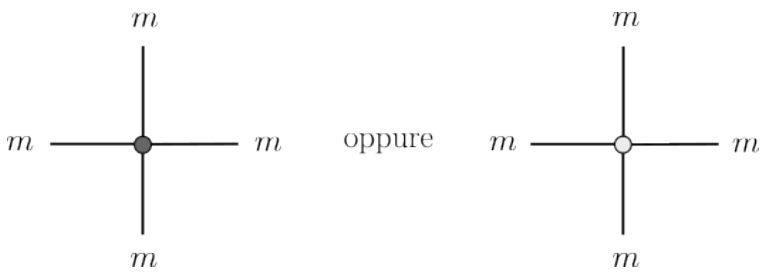
\includegraphics[width=0.6\linewidth]{Immagini/realizzazioni ACM.png}
    \caption{realizzazioni possibili nell'approssimazione di campo medio per un reticolo quadrato con $h = 0$.}
    \label{fig: realizzazioni ACM}
\end{figure}

Per consistenza, si deve anche richiedere che il valore medio di $s_i$ sia pari ad $m$, quindi
\begin{equation}
    \begin{split}
        \vmedio{s_i} = \sum_{\{s_i\}}s_i\frac{e^{\beta(Jqm + h)s_i}}{Z} &= \frac{e^{\beta(Jqm + h)} - e^{-\beta(Jqm + h)}}{Z} \\
        &= \frac{2\sinh{[\beta(Jqm + h)]}}{2\cosh{[\beta(Jqm + h)]}},
    \end{split}
\end{equation}
da cui si ricava l'``equazione di autoconsistenza''
\begin{equation}
\label{eq: equazione di atutoconsistenza}
    m = \tanh{[\beta(Jqm + h)]}.
\end{equation}
Questa è tutt'altro che un'equazione banale e non vale per qualsiasi valore di $m$, infatti è trascendente e determina i possibili valori di $m$ in funzione di $\beta$, $h$ e $J$. L'equazione \eqref{eq: equazione di atutoconsistenza} può essere risolta graficamente ponendo
\begin{equation}
    x = \beta Jqm + \beta h\quad\Longrightarrow\quad m = \frac{x - \beta h}{\beta Jq},
\end{equation}
permettendo di riscriverla come
\begin{equation}
    \frac{x - \beta h}{\beta Jq} = \tanh{x},
\end{equation}
facendo diventare il problema una ricerca grafica delle intersezioni tra le funzioni presenti ad ambo i membri, come mostrato in figura \ref{fig: soluzione grafica h = 0}. 
\begin{figure}[h]
    \centering
    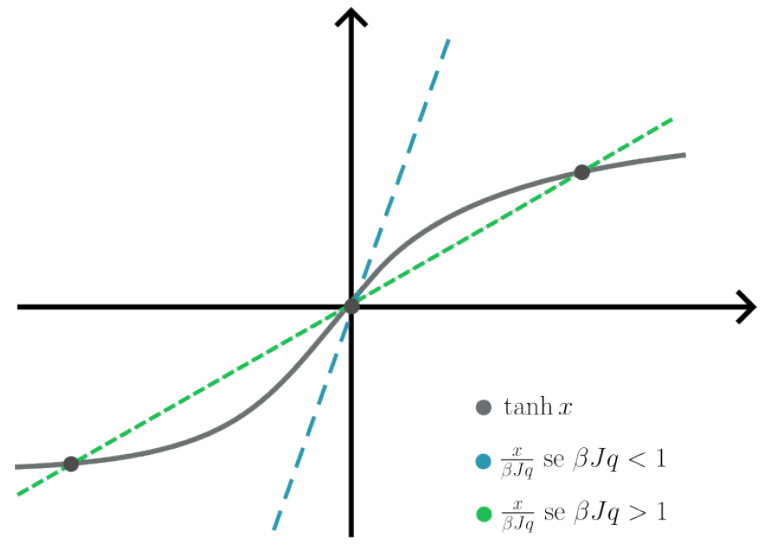
\includegraphics[width=0.5\linewidth]{Immagini/soluzione grafica h = 0.png}
    \caption{soluzione grafica per $h = 0$.}
    \label{fig: soluzione grafica h = 0}
\end{figure}
Si nota come la derivata della tangente $\tanh{x}$ sia pari ad uno nell'origine dato che
\begin{equation}
    \frac{d}{d x}(\tanh{x})\bigg|_{x=0} = \frac{1}{\coth^2{x}}\bigg|_{x=0} = 1,
\end{equation}
per cui la pendenza è di $45^\circ$. Quindi, nel caso in cui $h = 0$ si ha che:
\begin{enumerate}
    \item se $\beta J q > 1$, le due funzioni si incontrano solo in $x = 0$ ed anche $m = 0$;
    \item se $\beta J q < 1$, le due funzioni si incontrano in tre punti distinti ed $m$ può essere $m > 0$, $m < 0$ e $m = 0$.
\end{enumerate}
Pertanto, è possibile trovare delle soluzioni con magnetizzazione spontanea diversa da zero. Questo però succede soltanto quando le due fasi sono separate dal valore critico
\begin{equation}
\label{eq: K critico approssimazione campo medio}
    \beta J q = 1 \quad\Longleftrightarrow\quad K_c = \frac{1}{q} \quad\Longleftrightarrow\quad kT_c = Jq \equiv \frac{1}{\beta_c}.
\end{equation}
Questo risultato si avvicina a quello esatto o ai risultati numerici solo per $q$ alto, cioè per i reticoli regolari di dimensione alta, si raccolgono alcuni risultati in tabella \ref{tab: valori di K critico}.
\begin{table}[h]
    \centering
    \begin{tabular}{|c|c|c|}
    \hline
    $D$ & $K_c$ [campo medio] & $K_c$ [esatta o simulata] \\
    \hline
    1 & $1/2 = 0.5$   & $\infty$ \\
    \hline
    2 & $1/4 = 0.25$  & $\log(\sqrt{2}+1)/2$ \\
    \hline
    3 & $1/6 = 0.166$ & $0.221$ (MC) \\
    \hline
    4 & $1/8 = 0.125$ & $0.149$ (MC) \\
    \hline
    \end{tabular}
    \caption{valori di $K_c$ derivati dall'approssimazione di campo medio ed esatti, con (MC) si intende che la soluzione è stata trovata tramite il metodo di Monte Carlo.}
    \label{tab: valori di K critico}
\end{table}
Come si vede dalla medesima, per $D = 1$ il risultato derivante dall'approssimazione di campo medio è completamente sbagliato, poiché prevede una transizione di fase che non in realtà non c'è. Tuttavia, ci si aspetta che la soluzione si avvicini ad un risultato valido quando il reticolo è più connesso, ossia quando si hanno più primi vicini. 

D'altra parte, in presenza di $h > 0$ ci si aspetta invece che emerga una magnetizzazione, indotta dal campo esterno. In questo caso la soluzione grafica è mostrata in figura \ref{fig: soluzione grafica h > 0}. Si ha una rottura esplicita della simmetria $\Z_2$, dovuta alla presenza del termine non invariante $h\nsum_i s_i$ presente nell'hamiltoniana microscopica. Si ha poi una situazione simile, ma con il segno cambiato, se $h < 0$.
\begin{figure}[h]
    \centering
    \includegraphics[width=0.5\linewidth]{Immagini/soluzione grafica h > 0.png}
    \caption{soluzione grafica per $h > 0$.}
    \label{fig: soluzione grafica h > 0}
\end{figure}

\subsection{Equazione intorno al punto critico}
Ci si domanda se il campo medio possa prevedere anche gli indici critici nei pressi del punto critico. L'equazione di autoconsistenza \eqref{eq: equazione di atutoconsistenza} può essere scritta come
\begin{equation}
    \operatorname{arctanh}{m} = \beta Jq + \beta h = \frac{\beta}{\beta_c}m + \beta h,
\end{equation}
dove nel secondo passaggio si è usata l'equazione \eqref{eq: K critico approssimazione campo medio}. Intorno al punto critico, cioè con $\beta$ prossimo a $\beta_c$ e $h$ piccolo, si vede dalla soluzione grafica che $h$ ha una piccola magnetizzazione per ogni sito, per cui anche $m$ è piccolo. Quindi, si può sviluppare l'arcotangente iperbolica in modo da avere
\begin{equation}
    m + \frac{m^3}{3} + \cdots = m + \bigg(\frac{\beta}{\beta_c} - 1\bigg)m  + \beta h .
\end{equation}
in cui nell'ultimo termine si è trascurata la differenza perché $h$ è già piccolo. Inoltre, si ha la relazione 
\begin{equation}
    \bigg(\frac{\beta}{\beta_c} - 1\bigg) = \frac{T_c}{T} - 1  = \frac{T_c - T}{T_c} =  t \simeq \frac{T - T_c}{T_c} = -t
\end{equation}
dove è possibile confondere $T$ con $T_c$ a denominatore. Dunque, si arriva a 
\begin{equation}
    \frac{m^3}{3} \simeq  -mt + \frac{h}{Jq}.
\end{equation}
Si supponga ora di approcciare il punto critico dalla fase ordinata, cioè con $t < 0$, mantenendo $h = 0$, ossia di studiare la magnetizzazione spontanea al variare della temperatura. Quindi
\begin{equation}
\label{eq: valore di m per h = 0}
    \frac{m^3}{3} \simeq -mt\quad\Longrightarrow\quad m \simeq \sqrt{3}\,(-t)^{1/2},
\end{equation}
ovvero, in altri termini, il campo medio predice l'esponente critico
\begin{equation}
    \beta_{\mathrm{CM}} = \frac{1}{2} .
\end{equation}
Per l'approssimazione di campo medio, $\beta$ è sempre pari ad $1/2$, qualsiasi sia la dimensione. In $D = 1$ in realtà non c'è magnetizzazione spontanea, mentre in $D = 2$ il risultato esatto è $\beta_{\mathrm{exact}} = 1/8$ e in $D = 3$ i risultati numerici predicono $\beta_{\mathrm{numeric}} \sim 0.3$; pertanto, il campo medio inizia ad avvicinarsi al risultato corretto.

\subsubsection{Capacità termica}
Sempre nel caso in cui $h=0$, la predizione del campo medio per l'energia interna è
\begin{equation}
    E = \vmedio{H} = -J L m^2 = -\frac{J N q}{2} 3(-t) = \frac{3}{2} N J q \frac{T-T_c}{T_c},
\end{equation}
quando $m \neq 0$, cioè nella fase ordinata. Infine, dall'equazione \eqref{eq: K critico approssimazione campo medio} si ottiene
\begin{equation}
    E = 
    \begin{cases}
        \dfrac{3}{2} N k_B (T-T_c), \quad T < T_c,\,m\neq 0 \\[2ex]
        0, \quad T > T_c,\,m = 0
    \end{cases}
\end{equation}
dove $m = 0$ corrisponde alla fase disordinata. Dunque, la capacità termica è data da
\begin{equation}
    c_N = \frac{\p E}{\p T} =
    \begin{cases}
        \dfrac{3}{2} N k_B & T<T_c \\[2ex]
        0 & T>T_c
    \end{cases},
\end{equation}
il quale risulta evidentemente discontinuo. In particolare, per $D = 2$ la trattazione esatta prevede invece una divergenza logaritmica, con indice critico $\alpha_{\mathrm{exact}} = 0$.

\subsubsection{Suscettività magnetica}
Si supponga di accendere un campo esterno $h \ll 1$ in modo da poter calcolare la suscettività magnetica $\chi$. Nell'equazione
\begin{equation}
    \frac{m^3}{3} = -t m + \frac{h}{J q} + \cdots
\end{equation}
si può porre $m = m_0 + \epsilon$,  dove $m_0$ è la magnetizzazione spontanea che soddisfa l'equazione con $h = 0$ ed $\epsilon \ll 1$. In questo modo, si ha
\begin{equation}
\label{eq: equazione autoconsistenza punto critico}
    \begin{split}
        \frac{1}{3} ( m_0^3 + 3 m_0^2 \epsilon + 3 m_0 \epsilon^2 + \epsilon^3) &= -t(m_0 + \epsilon) + \frac{h}{Jq} \\
        m_0^2\epsilon &\simeq -t\epsilon + \frac{h}{Jq},
    \end{split}
\end{equation}
da cui, sostituendo ancora l'espressione \eqref{eq: valore di m per h = 0} per $m_0$, si trova
\begin{equation}
    -2t \epsilon = \frac{h}{J q} \quad\Longrightarrow\quad \epsilon = -\frac{h}{2Jqt}.
\end{equation}
Dunque, la suscettività magnetica è
\begin{equation}
    \chi = \frac{\p M}{\p B} = N \mu_B \frac{\p m}{\p h} = N \mu_B \frac{\p \epsilon}{\p h} = \frac{N \mu_B}{2 J q} (-t)^{-1},\quad T < T_c.
\end{equation}
Quindi, si è ottenuto un indice critico pari a $-1$. Se si ripetessero i calcoli nella fase simmetrica per $T > T_c$, si avrebbe $m_0 = 0$ e quindi $m = \epsilon \ll 1$, per cui l'equazione \eqref{eq: equazione autoconsistenza punto critico} si riduce a 
\begin{equation}
    \frac{\epsilon^3}{3} = -t \epsilon + \frac{h}{J q}
    \quad\Longrightarrow\quad \epsilon = \frac{h}{J q t},
\end{equation}
da cui si trova che la suscettività diventa
\begin{equation}
    \chi = N \mu_B \frac{\p \epsilon}{\p h} = \frac{N \mu_B}{J q} t^{-1},\quad T > T_c.
\end{equation}
Dunque, anche per la suscettività si trova una discontinuità
\begin{equation}
    \chi =
    \begin{cases}
        -\dfrac{N \mu_B}{2 J q}t^{-1},\quad T<T_c \\[2ex]
        \dfrac{N \mu_B}{J q} t^{-1},\quad T>T_c
    \end{cases}.
\end{equation}



\end{document}
